\documentclass[twoside]{book}

% Packages required by doxygen
\usepackage{fixltx2e}
\usepackage{calc}
\usepackage{doxygen}
\usepackage{graphicx}
\usepackage[utf8]{inputenc}
\usepackage{makeidx}
\usepackage{multicol}
\usepackage{multirow}
\PassOptionsToPackage{warn}{textcomp}
\usepackage{textcomp}
\usepackage[nointegrals]{wasysym}
\usepackage[table]{xcolor}

% Font selection
\usepackage[T1]{fontenc}
\usepackage{mathptmx}
\usepackage[scaled=.90]{helvet}
\usepackage{courier}
\usepackage{amssymb}
\usepackage{sectsty}
\renewcommand{\familydefault}{\sfdefault}
\allsectionsfont{%
  \fontseries{bc}\selectfont%
  \color{darkgray}%
}
\renewcommand{\DoxyLabelFont}{%
  \fontseries{bc}\selectfont%
  \color{darkgray}%
}
\newcommand{\+}{\discretionary{\mbox{\scriptsize$\hookleftarrow$}}{}{}}

% Page & text layout
\usepackage{geometry}
\geometry{%
  a4paper,%
  top=2.5cm,%
  bottom=2.5cm,%
  left=2.5cm,%
  right=2.5cm%
}
\tolerance=750
\hfuzz=15pt
\hbadness=750
\setlength{\emergencystretch}{15pt}
\setlength{\parindent}{0cm}
\setlength{\parskip}{0.2cm}
\makeatletter
\renewcommand{\paragraph}{%
  \@startsection{paragraph}{4}{0ex}{-1.0ex}{1.0ex}{%
    \normalfont\normalsize\bfseries\SS@parafont%
  }%
}
\renewcommand{\subparagraph}{%
  \@startsection{subparagraph}{5}{0ex}{-1.0ex}{1.0ex}{%
    \normalfont\normalsize\bfseries\SS@subparafont%
  }%
}
\makeatother

% Headers & footers
\usepackage{fancyhdr}
\pagestyle{fancyplain}
\fancyhead[LE]{\fancyplain{}{\bfseries\thepage}}
\fancyhead[CE]{\fancyplain{}{}}
\fancyhead[RE]{\fancyplain{}{\bfseries\leftmark}}
\fancyhead[LO]{\fancyplain{}{\bfseries\rightmark}}
\fancyhead[CO]{\fancyplain{}{}}
\fancyhead[RO]{\fancyplain{}{\bfseries\thepage}}
\fancyfoot[LE]{\fancyplain{}{}}
\fancyfoot[CE]{\fancyplain{}{}}
\fancyfoot[RE]{\fancyplain{}{\bfseries\scriptsize Generated on Sat Nov 22 2014 00\+:38\+:50 for My Project by Doxygen }}
\fancyfoot[LO]{\fancyplain{}{\bfseries\scriptsize Generated on Sat Nov 22 2014 00\+:38\+:50 for My Project by Doxygen }}
\fancyfoot[CO]{\fancyplain{}{}}
\fancyfoot[RO]{\fancyplain{}{}}
\renewcommand{\footrulewidth}{0.4pt}
\renewcommand{\chaptermark}[1]{%
  \markboth{#1}{}%
}
\renewcommand{\sectionmark}[1]{%
  \markright{\thesection\ #1}%
}

% Indices & bibliography
\usepackage{natbib}
\usepackage[titles]{tocloft}
\setcounter{tocdepth}{3}
\setcounter{secnumdepth}{5}
\makeindex

% Hyperlinks (required, but should be loaded last)
\usepackage{ifpdf}
\ifpdf
  \usepackage[pdftex,pagebackref=true]{hyperref}
\else
  \usepackage[ps2pdf,pagebackref=true]{hyperref}
\fi
\hypersetup{%
  colorlinks=true,%
  linkcolor=blue,%
  citecolor=blue,%
  unicode%
}

% Custom commands
\newcommand{\clearemptydoublepage}{%
  \newpage{\pagestyle{empty}\cleardoublepage}%
}


%===== C O N T E N T S =====

\begin{document}

% Titlepage & ToC
\hypersetup{pageanchor=false,
             bookmarks=true,
             bookmarksnumbered=true,
             pdfencoding=unicode
            }
\pagenumbering{roman}
\begin{titlepage}
\vspace*{7cm}
\begin{center}%
{\Large My Project }\\
\vspace*{1cm}
{\large Generated by Doxygen 1.8.8}\\
\vspace*{0.5cm}
{\small Sat Nov 22 2014 00:38:50}\\
\end{center}
\end{titlepage}
\clearemptydoublepage
\tableofcontents
\clearemptydoublepage
\pagenumbering{arabic}
\hypersetup{pageanchor=true}

%--- Begin generated contents ---
\chapter{Namespace Index}
\section{Namespace List}
Here is a list of all namespaces with brief descriptions\+:\begin{DoxyCompactList}
\item\contentsline{section}{\hyperlink{namespacejli}{jli} }{\pageref{namespacejli}}{}
\end{DoxyCompactList}

\chapter{Hierarchical Index}
\section{Class Hierarchy}
This inheritance list is sorted roughly, but not completely, alphabetically\+:\begin{DoxyCompactList}
\item Abstract\+Object\begin{DoxyCompactList}
\item \contentsline{section}{jli\+:\+:Abstract\+Decorator}{\pageref{classjli_1_1_abstract_decorator}}{}
\item \contentsline{section}{jli\+:\+:Abstract\+Factory\+Object}{\pageref{classjli_1_1_abstract_factory_object}}{}
\begin{DoxyCompactList}
\item \contentsline{section}{jli\+:\+:Abstract\+Builder}{\pageref{classjli_1_1_abstract_builder}}{}
\end{DoxyCompactList}
\end{DoxyCompactList}
\item \contentsline{section}{jli\+:\+:World}{\pageref{classjli_1_1_world}}{}
\item \contentsline{section}{jli\+:\+:World\+Factory}{\pageref{classjli_1_1_world_factory}}{}
\item \contentsline{section}{jli\+:\+:World\+Input}{\pageref{classjli_1_1_world_input}}{}
\item \contentsline{section}{jli\+:\+:World\+Lua\+Virtual\+Machine}{\pageref{classjli_1_1_world_lua_virtual_machine}}{}
\item \contentsline{section}{jli\+:\+:World\+My\+S\+Q\+L}{\pageref{classjli_1_1_world_my_s_q_l}}{}
\item \contentsline{section}{jli\+:\+:World\+Sound}{\pageref{classjli_1_1_world_sound}}{}
\end{DoxyCompactList}

\chapter{Class Index}
\section{Class List}
Here are the classes, structs, unions and interfaces with brief descriptions\+:\begin{DoxyCompactList}
\item\contentsline{section}{\hyperlink{class_abstract_behavior}{Abstract\+Behavior$<$ O\+W\+N\+E\+R\+\_\+\+T\+Y\+P\+E $>$} }{\pageref{class_abstract_behavior}}{}
\item\contentsline{section}{\hyperlink{class_abstract_factory}{Abstract\+Factory$<$ S\+I\+N\+G\+L\+E\+T\+O\+N\+S\+\_\+\+T\+Y\+P\+E, B\+A\+S\+E\+\_\+\+O\+B\+J\+E\+C\+T\+\_\+\+T\+Y\+P\+E $>$} }{\pageref{class_abstract_factory}}{}
\item\contentsline{section}{\hyperlink{class_abstract_shared_factory}{Abstract\+Shared\+Factory$<$ S\+I\+N\+G\+L\+E\+T\+O\+N\+S\+\_\+\+T\+Y\+P\+E, O\+B\+J\+E\+C\+T\+\_\+\+T\+Y\+P\+E $>$} }{\pageref{class_abstract_shared_factory}}{}
\item\contentsline{section}{\hyperlink{class_abstract_singleton}{Abstract\+Singleton$<$ S\+I\+N\+G\+L\+E\+T\+O\+N\+S\+\_\+\+T\+Y\+P\+E $>$} }{\pageref{class_abstract_singleton}}{}
\end{DoxyCompactList}

\chapter{File Index}
\section{File List}
Here is a list of all files with brief descriptions\+:\begin{DoxyCompactList}
\item\contentsline{section}{include/\hyperlink{_abstract_behavior_8h}{Abstract\+Behavior.\+h} }{\pageref{_abstract_behavior_8h}}{}
\item\contentsline{section}{include/\hyperlink{_abstract_builder_8h}{Abstract\+Builder.\+h} }{\pageref{_abstract_builder_8h}}{}
\item\contentsline{section}{include/\hyperlink{_abstract_decorator_8h}{Abstract\+Decorator.\+h} }{\pageref{_abstract_decorator_8h}}{}
\item\contentsline{section}{include/\hyperlink{_abstract_factory_8h}{Abstract\+Factory.\+h} }{\pageref{_abstract_factory_8h}}{}
\item\contentsline{section}{include/\hyperlink{_abstract_factory_object_8h}{Abstract\+Factory\+Object.\+h} }{\pageref{_abstract_factory_object_8h}}{}
\item\contentsline{section}{include/\hyperlink{_abstract_object_8h}{Abstract\+Object.\+h} }{\pageref{_abstract_object_8h}}{}
\item\contentsline{section}{include/\hyperlink{_abstract_shared_factory_8h}{Abstract\+Shared\+Factory.\+h} }{\pageref{_abstract_shared_factory_8h}}{}
\item\contentsline{section}{include/\hyperlink{_abstract_singleton_8h}{Abstract\+Singleton.\+h} }{\pageref{_abstract_singleton_8h}}{}
\item\contentsline{section}{include/\hyperlink{_abstract_state_8h}{Abstract\+State.\+h} }{\pageref{_abstract_state_8h}}{}
\item\contentsline{section}{include/\hyperlink{_abstract_state_machine_8h}{Abstract\+State\+Machine.\+h} }{\pageref{_abstract_state_machine_8h}}{}
\end{DoxyCompactList}

\chapter{Namespace Documentation}
\hypertarget{namespacejli}{\section{jli Namespace Reference}
\label{namespacejli}\index{jli@{jli}}
}
\subsection*{Classes}
\begin{DoxyCompactItemize}
\item 
class \hyperlink{classjli_1_1_abstract_builder}{Abstract\+Builder}
\item 
class \hyperlink{classjli_1_1_abstract_decorator}{Abstract\+Decorator}
\item 
class \hyperlink{classjli_1_1_abstract_factory_object}{Abstract\+Factory\+Object}
\item 
class \hyperlink{classjli_1_1_world}{World}
\item 
class \hyperlink{classjli_1_1_world_factory}{World\+Factory}
\item 
class \hyperlink{classjli_1_1_world_input}{World\+Input}
\item 
class \hyperlink{classjli_1_1_world_lua_virtual_machine}{World\+Lua\+Virtual\+Machine}
\item 
class \hyperlink{classjli_1_1_world_my_s_q_l}{World\+My\+S\+Q\+L}
\item 
class \hyperlink{classjli_1_1_world_sound}{World\+Sound}
\end{DoxyCompactItemize}
\subsection*{Enumerations}
\begin{DoxyCompactItemize}
\item 
enum \hyperlink{namespacejli_a11168ac254095f4ba73667ab33713b4f}{jli\+Object\+Enum\+Type} \{ \\*
\hyperlink{namespacejli_a11168ac254095f4ba73667ab33713b4fa64ba672259a65760b4ed49210521871f}{J\+L\+I\+\_\+\+O\+B\+J\+E\+C\+T\+\_\+\+T\+Y\+P\+E\+\_\+\+None} = 0, 
\hyperlink{namespacejli_a11168ac254095f4ba73667ab33713b4fa5d0124db06eb42f1bafeccf49a1df93a}{J\+L\+I\+\_\+\+O\+B\+J\+E\+C\+T\+\_\+\+T\+Y\+P\+E\+\_\+\+Action}, 
\hyperlink{namespacejli_a11168ac254095f4ba73667ab33713b4faf208272c41069b136b609b23e76d0653}{J\+L\+I\+\_\+\+O\+B\+J\+E\+C\+T\+\_\+\+T\+Y\+P\+E\+\_\+\+Action\+Builder}, 
\hyperlink{namespacejli_a11168ac254095f4ba73667ab33713b4fa6c336730aae3537f2f0e7fac0fe72de2}{J\+L\+I\+\_\+\+O\+B\+J\+E\+C\+T\+\_\+\+T\+Y\+P\+E\+\_\+\+Camera}, 
\\*
\hyperlink{namespacejli_a11168ac254095f4ba73667ab33713b4fa43c1c8354d86ce8b7b77b0557614caf1}{J\+L\+I\+\_\+\+O\+B\+J\+E\+C\+T\+\_\+\+T\+Y\+P\+E\+\_\+\+Camera\+Builder}, 
\hyperlink{namespacejli_a11168ac254095f4ba73667ab33713b4fa823ab588063f7fbde69b4affd73af75d}{J\+L\+I\+\_\+\+O\+B\+J\+E\+C\+T\+\_\+\+T\+Y\+P\+E\+\_\+\+Clock}, 
\hyperlink{namespacejli_a11168ac254095f4ba73667ab33713b4fa8078eb2cdd6168f3dc68ce380c32bea0}{J\+L\+I\+\_\+\+O\+B\+J\+E\+C\+T\+\_\+\+T\+Y\+P\+E\+\_\+\+Clock\+Builder}, 
\hyperlink{namespacejli_a11168ac254095f4ba73667ab33713b4facfcf5c7958e840c802319c9dc5052e97}{J\+L\+I\+\_\+\+O\+B\+J\+E\+C\+T\+\_\+\+T\+Y\+P\+E\+\_\+\+Collision\+Response}, 
\\*
\hyperlink{namespacejli_a11168ac254095f4ba73667ab33713b4fa7474dc229dd931b205dd5f0d8bb6867f}{J\+L\+I\+\_\+\+O\+B\+J\+E\+C\+T\+\_\+\+T\+Y\+P\+E\+\_\+\+Collision\+Response\+Builder}, 
\hyperlink{namespacejli_a11168ac254095f4ba73667ab33713b4fa8cc481c4c6831e7ffd4e90d663d30cf0}{J\+L\+I\+\_\+\+O\+B\+J\+E\+C\+T\+\_\+\+T\+Y\+P\+E\+\_\+\+Cubic\+Texture}, 
\hyperlink{namespacejli_a11168ac254095f4ba73667ab33713b4fab7852316145c6fbd4a33103ca6fb35a4}{J\+L\+I\+\_\+\+O\+B\+J\+E\+C\+T\+\_\+\+T\+Y\+P\+E\+\_\+\+Cubic\+Texture\+Builder}, 
\hyperlink{namespacejli_a11168ac254095f4ba73667ab33713b4fac54aa115e63cf54aea508ae3f13e540b}{J\+L\+I\+\_\+\+O\+B\+J\+E\+C\+T\+\_\+\+T\+Y\+P\+E\+\_\+\+Dynamic\+Physics\+Body}, 
\\*
\hyperlink{namespacejli_a11168ac254095f4ba73667ab33713b4fa8bf394969215d0e51d36216fd3e46ceb}{J\+L\+I\+\_\+\+O\+B\+J\+E\+C\+T\+\_\+\+T\+Y\+P\+E\+\_\+\+Dynamic\+Physics\+Body\+Builder}, 
\hyperlink{namespacejli_a11168ac254095f4ba73667ab33713b4fa7556628e9c3e2d172e0be379d0f559ae}{J\+L\+I\+\_\+\+O\+B\+J\+E\+C\+T\+\_\+\+T\+Y\+P\+E\+\_\+\+Geometry}, 
\hyperlink{namespacejli_a11168ac254095f4ba73667ab33713b4fa7c6039114e04ae77e17fff7eb367787f}{J\+L\+I\+\_\+\+O\+B\+J\+E\+C\+T\+\_\+\+T\+Y\+P\+E\+\_\+\+Geometry\+Builder}, 
\hyperlink{namespacejli_a11168ac254095f4ba73667ab33713b4fa53e8221ae0e3d18b5031babc8301668a}{J\+L\+I\+\_\+\+O\+B\+J\+E\+C\+T\+\_\+\+T\+Y\+P\+E\+\_\+\+Ghost\+Physics\+Body}, 
\\*
\hyperlink{namespacejli_a11168ac254095f4ba73667ab33713b4faf96b54ae51d930234e3d29ce4a8fc030}{J\+L\+I\+\_\+\+O\+B\+J\+E\+C\+T\+\_\+\+T\+Y\+P\+E\+\_\+\+Ghost\+Physics\+Body\+Builder}, 
\hyperlink{namespacejli_a11168ac254095f4ba73667ab33713b4faacc9012b0424691b11ad9f7b6357e452}{J\+L\+I\+\_\+\+O\+B\+J\+E\+C\+T\+\_\+\+T\+Y\+P\+E\+\_\+\+Kinematic\+Physics\+Body}, 
\hyperlink{namespacejli_a11168ac254095f4ba73667ab33713b4faae77bd17845d9df9949aacd3c7a5ffdf}{J\+L\+I\+\_\+\+O\+B\+J\+E\+C\+T\+\_\+\+T\+Y\+P\+E\+\_\+\+Kinematic\+Physics\+Body\+Builder}, 
\hyperlink{namespacejli_a11168ac254095f4ba73667ab33713b4fafd517ccec226398fa5f4746fd101f5e1}{J\+L\+I\+\_\+\+O\+B\+J\+E\+C\+T\+\_\+\+T\+Y\+P\+E\+\_\+\+Light}, 
\\*
\hyperlink{namespacejli_a11168ac254095f4ba73667ab33713b4fa95901f2c0a5dd0b2c26ec52f9af65e8b}{J\+L\+I\+\_\+\+O\+B\+J\+E\+C\+T\+\_\+\+T\+Y\+P\+E\+\_\+\+Light\+Builder}, 
\hyperlink{namespacejli_a11168ac254095f4ba73667ab33713b4fa692a9f5096cef91cf026e14d97d06c6e}{J\+L\+I\+\_\+\+O\+B\+J\+E\+C\+T\+\_\+\+T\+Y\+P\+E\+\_\+\+Material}, 
\hyperlink{namespacejli_a11168ac254095f4ba73667ab33713b4fae5eea4413d056fcb870d60c01f847ce5}{J\+L\+I\+\_\+\+O\+B\+J\+E\+C\+T\+\_\+\+T\+Y\+P\+E\+\_\+\+Material\+Builder}, 
\hyperlink{namespacejli_a11168ac254095f4ba73667ab33713b4fada3514d2b6b1cf22366c6edd4263c373}{J\+L\+I\+\_\+\+O\+B\+J\+E\+C\+T\+\_\+\+T\+Y\+P\+E\+\_\+\+Material\+Property}, 
\\*
\hyperlink{namespacejli_a11168ac254095f4ba73667ab33713b4fa51abac2dafb0f514ac5725f77da785e8}{J\+L\+I\+\_\+\+O\+B\+J\+E\+C\+T\+\_\+\+T\+Y\+P\+E\+\_\+\+Material\+Property\+Builder}, 
\hyperlink{namespacejli_a11168ac254095f4ba73667ab33713b4fa5e72138a8e03782a9872245990e2e550}{J\+L\+I\+\_\+\+O\+B\+J\+E\+C\+T\+\_\+\+T\+Y\+P\+E\+\_\+\+Node}, 
\hyperlink{namespacejli_a11168ac254095f4ba73667ab33713b4fad53a1cfc18dc8042c56cef7aad1845fa}{J\+L\+I\+\_\+\+O\+B\+J\+E\+C\+T\+\_\+\+T\+Y\+P\+E\+\_\+\+Node\+Builder}, 
\hyperlink{namespacejli_a11168ac254095f4ba73667ab33713b4fa06c51ddae796d13d594a25b2c62f48cf}{J\+L\+I\+\_\+\+O\+B\+J\+E\+C\+T\+\_\+\+T\+Y\+P\+E\+\_\+\+Node\+State}, 
\\*
\hyperlink{namespacejli_a11168ac254095f4ba73667ab33713b4fafb2f29fe89ceae02706926076401e5ff}{J\+L\+I\+\_\+\+O\+B\+J\+E\+C\+T\+\_\+\+T\+Y\+P\+E\+\_\+\+Node\+State\+Builder}, 
\hyperlink{namespacejli_a11168ac254095f4ba73667ab33713b4fa0c9ae614eee253fb1c258abeba0abb19}{J\+L\+I\+\_\+\+O\+B\+J\+E\+C\+T\+\_\+\+T\+Y\+P\+E\+\_\+\+Node\+State\+Machine}, 
\hyperlink{namespacejli_a11168ac254095f4ba73667ab33713b4fa3ff1ed55ac7bb4f4a99679ce1fce14a7}{J\+L\+I\+\_\+\+O\+B\+J\+E\+C\+T\+\_\+\+T\+Y\+P\+E\+\_\+\+Node\+State\+Machine\+Builder}, 
\hyperlink{namespacejli_a11168ac254095f4ba73667ab33713b4fab1b48f3c21a43d9fe2e3bbcb6515b059}{J\+L\+I\+\_\+\+O\+B\+J\+E\+C\+T\+\_\+\+T\+Y\+P\+E\+\_\+\+Particle\+Emitter}, 
\\*
\hyperlink{namespacejli_a11168ac254095f4ba73667ab33713b4facad92c58f5440e8cf31f05ba9ce3bb78}{J\+L\+I\+\_\+\+O\+B\+J\+E\+C\+T\+\_\+\+T\+Y\+P\+E\+\_\+\+Particle\+Emitter\+Builder}, 
\hyperlink{namespacejli_a11168ac254095f4ba73667ab33713b4fa15cae65abb2827515504c48b94685aaa}{J\+L\+I\+\_\+\+O\+B\+J\+E\+C\+T\+\_\+\+T\+Y\+P\+E\+\_\+\+Physics\+Contact}, 
\hyperlink{namespacejli_a11168ac254095f4ba73667ab33713b4fa56ea0dbaab9c999e0ef6d028223d5739}{J\+L\+I\+\_\+\+O\+B\+J\+E\+C\+T\+\_\+\+T\+Y\+P\+E\+\_\+\+Physics\+Contact\+Builder}, 
\hyperlink{namespacejli_a11168ac254095f4ba73667ab33713b4fa50c6ebf8c7c234ccb939729141e88f62}{J\+L\+I\+\_\+\+O\+B\+J\+E\+C\+T\+\_\+\+T\+Y\+P\+E\+\_\+\+Physics\+Field}, 
\\*
\hyperlink{namespacejli_a11168ac254095f4ba73667ab33713b4fa3e2efbeef070d670dfff0f5d37cdb298}{J\+L\+I\+\_\+\+O\+B\+J\+E\+C\+T\+\_\+\+T\+Y\+P\+E\+\_\+\+Physics\+Field\+Builder}, 
\hyperlink{namespacejli_a11168ac254095f4ba73667ab33713b4fac082f64545107452af9853ba7e19d5c4}{J\+L\+I\+\_\+\+O\+B\+J\+E\+C\+T\+\_\+\+T\+Y\+P\+E\+\_\+\+Physics\+Shape}, 
\hyperlink{namespacejli_a11168ac254095f4ba73667ab33713b4fa0c10cc7af6eea2138dd84d1da4695ed2}{J\+L\+I\+\_\+\+O\+B\+J\+E\+C\+T\+\_\+\+T\+Y\+P\+E\+\_\+\+Physics\+Shape\+Builder}, 
\hyperlink{namespacejli_a11168ac254095f4ba73667ab33713b4fac8ae5ac026d13828082da80a9b530e8b}{J\+L\+I\+\_\+\+O\+B\+J\+E\+C\+T\+\_\+\+T\+Y\+P\+E\+\_\+\+Physics\+World}, 
\\*
\hyperlink{namespacejli_a11168ac254095f4ba73667ab33713b4fad66acbd298aef9c201be72c6f8851452}{J\+L\+I\+\_\+\+O\+B\+J\+E\+C\+T\+\_\+\+T\+Y\+P\+E\+\_\+\+Physics\+World\+Builder}, 
\hyperlink{namespacejli_a11168ac254095f4ba73667ab33713b4faf241f6c763603fc08118143a1dad3eb0}{J\+L\+I\+\_\+\+O\+B\+J\+E\+C\+T\+\_\+\+T\+Y\+P\+E\+\_\+\+Resource}, 
\hyperlink{namespacejli_a11168ac254095f4ba73667ab33713b4fa028bf9a736b34ef0911c0d529530b46e}{J\+L\+I\+\_\+\+O\+B\+J\+E\+C\+T\+\_\+\+T\+Y\+P\+E\+\_\+\+Resource\+Builder}, 
\hyperlink{namespacejli_a11168ac254095f4ba73667ab33713b4faa1e1d08c0c3839422d166854f5bc284c}{J\+L\+I\+\_\+\+O\+B\+J\+E\+C\+T\+\_\+\+T\+Y\+P\+E\+\_\+\+Rigid\+Physics\+Body}, 
\\*
\hyperlink{namespacejli_a11168ac254095f4ba73667ab33713b4faf50d5fcce806b6aaed0de631368fcbc8}{J\+L\+I\+\_\+\+O\+B\+J\+E\+C\+T\+\_\+\+T\+Y\+P\+E\+\_\+\+Rigid\+Physics\+Body\+Builder}, 
\hyperlink{namespacejli_a11168ac254095f4ba73667ab33713b4fac654a5c20d502e914f60b98a533fae5b}{J\+L\+I\+\_\+\+O\+B\+J\+E\+C\+T\+\_\+\+T\+Y\+P\+E\+\_\+\+Scene}, 
\hyperlink{namespacejli_a11168ac254095f4ba73667ab33713b4fa49215a175711ce4e497b38077d1f218d}{J\+L\+I\+\_\+\+O\+B\+J\+E\+C\+T\+\_\+\+T\+Y\+P\+E\+\_\+\+Scene\+Builder}, 
\hyperlink{namespacejli_a11168ac254095f4ba73667ab33713b4fa6d9bc7667714266f0ec6ac1b3c724740}{J\+L\+I\+\_\+\+O\+B\+J\+E\+C\+T\+\_\+\+T\+Y\+P\+E\+\_\+\+Scene\+State}, 
\\*
\hyperlink{namespacejli_a11168ac254095f4ba73667ab33713b4fa909db2a11a1e1aa837b16c62efa0ad60}{J\+L\+I\+\_\+\+O\+B\+J\+E\+C\+T\+\_\+\+T\+Y\+P\+E\+\_\+\+Scene\+State\+Builder}, 
\hyperlink{namespacejli_a11168ac254095f4ba73667ab33713b4fa48bb932825433539200a3b65b56667fb}{J\+L\+I\+\_\+\+O\+B\+J\+E\+C\+T\+\_\+\+T\+Y\+P\+E\+\_\+\+Scene\+State\+Machine}, 
\hyperlink{namespacejli_a11168ac254095f4ba73667ab33713b4fa5c01dbd937bfa0cf3c9ddf3ec72a801f}{J\+L\+I\+\_\+\+O\+B\+J\+E\+C\+T\+\_\+\+T\+Y\+P\+E\+\_\+\+Scene\+State\+Machine\+Builder}, 
\hyperlink{namespacejli_a11168ac254095f4ba73667ab33713b4fadffaeaeba48e4c617f031631f56b7971}{J\+L\+I\+\_\+\+O\+B\+J\+E\+C\+T\+\_\+\+T\+Y\+P\+E\+\_\+\+Soft\+Physics\+Body}, 
\\*
\hyperlink{namespacejli_a11168ac254095f4ba73667ab33713b4fa4f63929bcaf9fd00fb2549e4b4c16b8e}{J\+L\+I\+\_\+\+O\+B\+J\+E\+C\+T\+\_\+\+T\+Y\+P\+E\+\_\+\+Soft\+Physics\+Body\+Builder}, 
\hyperlink{namespacejli_a11168ac254095f4ba73667ab33713b4fa8439ad2ae89b3e4132d5ece3fbd86df5}{J\+L\+I\+\_\+\+O\+B\+J\+E\+C\+T\+\_\+\+T\+Y\+P\+E\+\_\+\+Sound}, 
\hyperlink{namespacejli_a11168ac254095f4ba73667ab33713b4fa3d2fceddab6464321da384f1cef2f989}{J\+L\+I\+\_\+\+O\+B\+J\+E\+C\+T\+\_\+\+T\+Y\+P\+E\+\_\+\+Sound\+Builder}, 
\hyperlink{namespacejli_a11168ac254095f4ba73667ab33713b4fa112f0910199296fb1e54cb216e580a44}{J\+L\+I\+\_\+\+O\+B\+J\+E\+C\+T\+\_\+\+T\+Y\+P\+E\+\_\+\+Texture}, 
\\*
\hyperlink{namespacejli_a11168ac254095f4ba73667ab33713b4fa10494179b60406fc7fcc8519749963cf}{J\+L\+I\+\_\+\+O\+B\+J\+E\+C\+T\+\_\+\+T\+Y\+P\+E\+\_\+\+Texture\+Builder}, 
\hyperlink{namespacejli_a11168ac254095f4ba73667ab33713b4fa6ebb52bf397ab0251c596e0c378fcbde}{J\+L\+I\+\_\+\+O\+B\+J\+E\+C\+T\+\_\+\+T\+Y\+P\+E\+\_\+\+World\+State}, 
\hyperlink{namespacejli_a11168ac254095f4ba73667ab33713b4faf2c29a63420b028a4ab247347b134968}{J\+L\+I\+\_\+\+O\+B\+J\+E\+C\+T\+\_\+\+T\+Y\+P\+E\+\_\+\+World\+State\+Builder}, 
\hyperlink{namespacejli_a11168ac254095f4ba73667ab33713b4faec7d71f74b14a31ecf4984b2e109edce}{J\+L\+I\+\_\+\+O\+B\+J\+E\+C\+T\+\_\+\+T\+Y\+P\+E\+\_\+\+World\+State\+Machine}, 
\\*
\hyperlink{namespacejli_a11168ac254095f4ba73667ab33713b4fa5e7f3ca8449bf25022f1b270b15063d3}{J\+L\+I\+\_\+\+O\+B\+J\+E\+C\+T\+\_\+\+T\+Y\+P\+E\+\_\+\+World\+State\+Machine\+Builder}, 
\hyperlink{namespacejli_a11168ac254095f4ba73667ab33713b4fa615463e81f6742b668633f9ccf74fccc}{J\+L\+I\+\_\+\+O\+B\+J\+E\+C\+T\+\_\+\+T\+Y\+P\+E\+\_\+\+Number\+Of\+Types}
 \}
\end{DoxyCompactItemize}
\subsection*{Functions}
\begin{DoxyCompactItemize}
\item 
\hyperlink{namespacejli_a5cb9f42798ccca4b6de51fe827ade095}{A\+T\+T\+R\+I\+B\+U\+T\+E\+\_\+\+A\+L\+I\+G\+N\+E\+D16} (class) Abstract\+Object
\item 
\hyperlink{namespacejli_a4eb9a23f0614497a7922d323a49cb822}{Abstract\+Physics\+Body} ()
\item 
\hyperlink{namespacejli_ad1a3c0146786fe6995fb9696c653555f}{Abstract\+Physics\+Body} (const \hyperlink{classjli_1_1_abstract_builder}{Abstract\+Builder} \&)
\item 
\hyperlink{namespacejli_a42235253cee125ef6fe3f35d61cb6a12}{Abstract\+Physics\+Body} (const Abstract\+Physics\+Body \&)
\item 
\hyperlink{namespacejli_a570a0b81268f888f69ad4c8b7fe6edae}{B\+T\+\_\+\+D\+E\+C\+L\+A\+R\+E\+\_\+\+A\+L\+I\+G\+N\+E\+D\+\_\+\+A\+L\+L\+O\+C\+A\+T\+O\+R} ()
\item 
virtual \hyperlink{namespacejli_aacaf3d149e42af3ba68c1225ccbe6797}{$\sim$\+Abstract\+Physics\+Body} ()
\item 
\hyperlink{namespacejli_a4eb9a23f0614497a7922d323a49cb822}{Abstract\+Physics\+Body} \& \hyperlink{namespacejli_abf374f753c2ae3833479fc522c07b7a9}{operator=} (const \hyperlink{namespacejli_a4eb9a23f0614497a7922d323a49cb822}{Abstract\+Physics\+Body} \&)
\item 
virtual s32 \hyperlink{namespacejli_a643ba9aff12ba46ade9719f4d8c08303}{calculate\+Serialize\+Buffer\+Size} () const =0
\item 
virtual void \hyperlink{namespacejli_aa823f0f9cca7324a986925864ae004f6}{serialize} (void $\ast$, bt\+Serializer $\ast$) const =0
\item 
virtual const char $\ast$ \hyperlink{namespacejli_a0fd7c3459b7eb61032050c78a9d48d65}{get\+Class\+Name} () const =0
\item 
virtual u32 \hyperlink{namespacejli_ab742f1c07eed63b74053aa01c3193d1f}{get\+Type} () const =0
\item 
{\footnotesize template$<$class O\+B\+J\+E\+C\+T\+\_\+\+T\+Y\+P\+E $>$ }\\\hyperlink{namespacejli_a5cb9f42798ccca4b6de51fe827ade095}{A\+T\+T\+R\+I\+B\+U\+T\+E\+\_\+\+A\+L\+I\+G\+N\+E\+D16}(class) \\*
Abstract\+State \hyperlink{namespacejli_afb90c6843a57abb6648df522fd034666}{Abstract\+State} (const \hyperlink{classjli_1_1_abstract_builder}{Abstract\+Builder} \&builder)
\item 
\hyperlink{namespacejli_ac1726cb5b995ec49ba12eea96abfc7b2}{Abstract\+State} (const Abstract\+State \&copy)
\item 
virtual \hyperlink{namespacejli_a4f29ddbfb1999ccb9059334002f37aaf}{$\sim$\+Abstract\+State} ()=0
\item 
\hyperlink{namespacejli_afb90c6843a57abb6648df522fd034666}{Abstract\+State} \& \hyperlink{namespacejli_a11ea974b98a56570306c45017bb5fcf4}{operator=} (const \hyperlink{namespacejli_afb90c6843a57abb6648df522fd034666}{Abstract\+State} \&)
\item 
virtual bool \hyperlink{namespacejli_a03fa79fbaafd83709515e1115c5a3986}{is\+Finished} () const 
\item 
virtual void \hyperlink{namespacejli_abe513ad11f4f190e62b972f4f8893aea}{enable\+Finished} (const bool=true)
\item 
virtual bool \hyperlink{namespacejli_ac98ddd4e4925a857a8935b40178b2718}{is\+In\+Use} () const 
\item 
virtual void \hyperlink{namespacejli_a28a9fe0627a5e67e2e4a15a3663f7bc4}{enable\+In\+Use} (const bool=true)
\item 
virtual void \hyperlink{namespacejli_aaa622c9ff88b18070c8c1c970b4a26f8}{enter} (O\+B\+J\+E\+C\+T\+\_\+\+T\+Y\+P\+E $\ast$)=0
\item 
virtual void \hyperlink{namespacejli_a922c317a977284f6b6e24ed5c655dd12}{update} (O\+B\+J\+E\+C\+T\+\_\+\+T\+Y\+P\+E $\ast$, f32)=0
\item 
virtual void \hyperlink{namespacejli_ad265e81449125b1850fe3a2874dae6f6}{exit} (O\+B\+J\+E\+C\+T\+\_\+\+T\+Y\+P\+E $\ast$)=0
\item 
virtual bool \hyperlink{namespacejli_ad9966e101b766e590473468c68125124}{on\+Message} (O\+B\+J\+E\+C\+T\+\_\+\+T\+Y\+P\+E $\ast$, const Telegram \&)=0
\item 
\hyperlink{namespacejli_ac1d6edc4f796157e771fb531302807c5}{Action} ()
\item 
\hyperlink{namespacejli_a372d9d21f05940e5e2e7728e51e5497e}{Action} (const \hyperlink{classjli_1_1_abstract_builder}{Abstract\+Builder} \&)
\item 
\hyperlink{namespacejli_a56537e2852192599346977eae126cf3f}{Action} (const Action \&)
\item 
virtual \hyperlink{namespacejli_a366502b547b6ed3de30f23020a65df04}{$\sim$\+Action} ()
\item 
\hyperlink{namespacejli_ac1d6edc4f796157e771fb531302807c5}{Action} \& \hyperlink{namespacejli_a3652a77b1603e782ad8ac9ff69eb0f83}{operator=} (const \hyperlink{namespacejli_ac1d6edc4f796157e771fb531302807c5}{Action} \&)
\item 
\hyperlink{namespacejli_add5250909a3a5a38d28295b426e43da7}{Action\+Builder} ()
\item 
\hyperlink{namespacejli_a96508fbaf421e7088d0213d649abf7ba}{Action\+Builder} (const Action\+Builder \&)
\item 
\hyperlink{namespacejli_ab6f83e83f1cecc616fbcc6dab3d26954}{Action\+Builder} (const \hyperlink{classjli_1_1_abstract_builder}{Abstract\+Builder} \&)
\item 
virtual \hyperlink{namespacejli_ab2e77266449aea2fbf9db5435931dc84}{$\sim$\+Action\+Builder} ()
\item 
\hyperlink{namespacejli_add5250909a3a5a38d28295b426e43da7}{Action\+Builder} \& \hyperlink{namespacejli_a52eac4944ed6adea3292bb7646e89bb1}{operator=} (const \hyperlink{namespacejli_add5250909a3a5a38d28295b426e43da7}{Action\+Builder} \&)
\item 
virtual u32 \hyperlink{namespacejli_ad74268a8f5493ee3df657a346cd64d30}{get\+Object\+Type} () const 
\item 
\hyperlink{namespacejli_ad3d15c9bf468345cc46e47bf7dd7d3e3}{Camera} ()
\item 
\hyperlink{namespacejli_a97fa95992b76788ae3feb7c62ddd6168}{Camera} (const \hyperlink{classjli_1_1_abstract_builder}{Abstract\+Builder} \&)
\item 
\hyperlink{namespacejli_a987bfeb3ffde7a3a032e131c6c356c53}{Camera} (const Camera \&)
\item 
virtual \hyperlink{namespacejli_a9407d365ccc6d206674e5a5869758943}{$\sim$\+Camera} ()
\item 
\hyperlink{namespacejli_ad3d15c9bf468345cc46e47bf7dd7d3e3}{Camera} \& \hyperlink{namespacejli_ae0ca0605362d0f66744c6b8c44e73adb}{operator=} (const \hyperlink{namespacejli_ad3d15c9bf468345cc46e47bf7dd7d3e3}{Camera} \&)
\item 
\hyperlink{namespacejli_ac774207b2ca46f60adc7d58d5252ebec}{Camera\+Builder} ()
\item 
\hyperlink{namespacejli_a8fe2558f8fe1d572700b414f9c0ccdf0}{Camera\+Builder} (const Camera\+Builder \&)
\item 
\hyperlink{namespacejli_a2dd10cbeedd42092b35159fd713834f3}{Camera\+Builder} (const \hyperlink{classjli_1_1_abstract_builder}{Abstract\+Builder} \&)
\item 
virtual \hyperlink{namespacejli_af4eb98dba938417574ac1607e82a5da6}{$\sim$\+Camera\+Builder} ()
\item 
\hyperlink{namespacejli_ac774207b2ca46f60adc7d58d5252ebec}{Camera\+Builder} \& \hyperlink{namespacejli_a75dbc7e82adc58eea850e84fbc0db767}{operator=} (const \hyperlink{namespacejli_ac774207b2ca46f60adc7d58d5252ebec}{Camera\+Builder} \&)
\item 
\hyperlink{namespacejli_af69056b00744493ba074ef13e82b0bec}{Clock} ()
\item 
\hyperlink{namespacejli_a334855814780bf6b3108045f5bf20c40}{Clock} (const \hyperlink{classjli_1_1_abstract_builder}{Abstract\+Builder} \&)
\item 
\hyperlink{namespacejli_a7ce97585499e25f837d2b1a14a4af4ce}{Clock} (const Clock \&)
\item 
virtual \hyperlink{namespacejli_aad1ce3f2fd2e7830b0fed2a040647134}{$\sim$\+Clock} ()
\item 
\hyperlink{namespacejli_af69056b00744493ba074ef13e82b0bec}{Clock} \& \hyperlink{namespacejli_a1ff847178b6d16582b0c1ca11c646090}{operator=} (const \hyperlink{namespacejli_af69056b00744493ba074ef13e82b0bec}{Clock} \&)
\item 
\hyperlink{namespacejli_af9355f336950e30078eac279a96a7375}{Clock\+Builder} ()
\item 
\hyperlink{namespacejli_a59f88ada47f2f75bad05d58b79344dd1}{Clock\+Builder} (const Clock\+Builder \&)
\item 
\hyperlink{namespacejli_a6eb2d97c9c7e59378580ac6637daf99c}{Clock\+Builder} (const \hyperlink{classjli_1_1_abstract_builder}{Abstract\+Builder} \&)
\item 
virtual \hyperlink{namespacejli_aedf4fd3834c4b8806fa9a257d496df30}{$\sim$\+Clock\+Builder} ()
\item 
\hyperlink{namespacejli_af9355f336950e30078eac279a96a7375}{Clock\+Builder} \& \hyperlink{namespacejli_ab2df9e6084dba760e66f854ddaed69ff}{operator=} (const \hyperlink{namespacejli_af9355f336950e30078eac279a96a7375}{Clock\+Builder} \&)
\item 
\hyperlink{namespacejli_ade7f2a4f2880c0d04736c3677ff61c1a}{Collision\+Response} ()
\item 
\hyperlink{namespacejli_a5253cd6674cbb5acad943c6652f1941d}{Collision\+Response} (const \hyperlink{classjli_1_1_abstract_builder}{Abstract\+Builder} \&)
\item 
\hyperlink{namespacejli_aa016cba40071d115792a6ab008cc30c5}{Collision\+Response} (const Collision\+Response \&)
\item 
virtual \hyperlink{namespacejli_ad8c3da9eb7afceee20db6db716280ce0}{$\sim$\+Collision\+Response} ()
\item 
\hyperlink{namespacejli_ade7f2a4f2880c0d04736c3677ff61c1a}{Collision\+Response} \& \hyperlink{namespacejli_ac9b74cda6418ae6175a9178669229562}{operator=} (const \hyperlink{namespacejli_ade7f2a4f2880c0d04736c3677ff61c1a}{Collision\+Response} \&)
\item 
\hyperlink{namespacejli_aba46547ac77fd775617b1e9c5c4c3807}{Collision\+Response\+Builder} ()
\item 
\hyperlink{namespacejli_ade55a82bdee00c30fda3b15d26caca25}{Collision\+Response\+Builder} (const Collision\+Response\+Builder \&)
\item 
\hyperlink{namespacejli_a921545297d17ff8c23fcab0bb4a2a67f}{Collision\+Response\+Builder} (const \hyperlink{classjli_1_1_abstract_builder}{Abstract\+Builder} \&)
\item 
virtual \hyperlink{namespacejli_a92b1a214131802c7cde48d0908a810e1}{$\sim$\+Collision\+Response\+Builder} ()
\item 
\hyperlink{namespacejli_aba46547ac77fd775617b1e9c5c4c3807}{Collision\+Response\+Builder} \& \hyperlink{namespacejli_ad3d3c1fad0e4aea9e098049aded55a07}{operator=} (const \hyperlink{namespacejli_aba46547ac77fd775617b1e9c5c4c3807}{Collision\+Response\+Builder} \&)
\item 
\hyperlink{namespacejli_a1d29d42a67cba1e824b2bbef37ad3ac7}{Cubic\+Texture} ()
\item 
\hyperlink{namespacejli_afcdf119bfd2e7541a5d202805d6f07ad}{Cubic\+Texture} (const \hyperlink{classjli_1_1_abstract_builder}{Abstract\+Builder} \&)
\item 
\hyperlink{namespacejli_a224b5438fe535ded0127d92bd9e595dc}{Cubic\+Texture} (const Cubic\+Texture \&)
\item 
virtual \hyperlink{namespacejli_a64fcdd5d3fead8d1be7f29da5ee2d330}{$\sim$\+Cubic\+Texture} ()
\item 
\hyperlink{namespacejli_a1d29d42a67cba1e824b2bbef37ad3ac7}{Cubic\+Texture} \& \hyperlink{namespacejli_ad7545b9768425cea8f01be5265c970c8}{operator=} (const \hyperlink{namespacejli_a1d29d42a67cba1e824b2bbef37ad3ac7}{Cubic\+Texture} \&)
\item 
\hyperlink{namespacejli_a2a86125c6b724a9338c6950c2d88ba63}{Cubic\+Texture\+Builder} ()
\item 
\hyperlink{namespacejli_a5f17b78a514c78975beb02040161f8f7}{Cubic\+Texture\+Builder} (const Cubic\+Texture\+Builder \&)
\item 
\hyperlink{namespacejli_a2640ff46287ef90c9cbe4d81d3e87c46}{Cubic\+Texture\+Builder} (const \hyperlink{classjli_1_1_abstract_builder}{Abstract\+Builder} \&)
\item 
virtual \hyperlink{namespacejli_aa2eeb6eccc9f5dd78d8a050d1c00eafc}{$\sim$\+Cubic\+Texture\+Builder} ()
\item 
\hyperlink{namespacejli_a2a86125c6b724a9338c6950c2d88ba63}{Cubic\+Texture\+Builder} \& \hyperlink{namespacejli_a23318afe35b09c9c6d4fb466724ad63a}{operator=} (const \hyperlink{namespacejli_a2a86125c6b724a9338c6950c2d88ba63}{Cubic\+Texture\+Builder} \&)
\item 
\hyperlink{namespacejli_a3bc1a43f8a3bfe33e3874a74ebfde685}{Dynamic\+Physics\+Body} ()
\item 
\hyperlink{namespacejli_a624a3cdacc2bbdd8f5aa1bfa94d65e78}{Dynamic\+Physics\+Body} (const \hyperlink{classjli_1_1_abstract_builder}{Abstract\+Builder} \&)
\item 
\hyperlink{namespacejli_a3bdc7905c274142d7f2930b7632bb0bc}{Dynamic\+Physics\+Body} (const Dynamic\+Physics\+Body \&)
\item 
virtual \hyperlink{namespacejli_a69f8874be747ab0e2f52c063ff30cf8a}{$\sim$\+Dynamic\+Physics\+Body} ()
\item 
\hyperlink{namespacejli_a3bc1a43f8a3bfe33e3874a74ebfde685}{Dynamic\+Physics\+Body} \& \hyperlink{namespacejli_aebf62cef126edcd79bdabcfa87a74074}{operator=} (const \hyperlink{namespacejli_a3bc1a43f8a3bfe33e3874a74ebfde685}{Dynamic\+Physics\+Body} \&)
\item 
\hyperlink{namespacejli_a2f8ceeb7f6753810b5778f1f4e2ffcff}{Dynamic\+Physics\+Body\+Builder} ()
\item 
\hyperlink{namespacejli_a925718f179e05461f123aec7d49e2302}{Dynamic\+Physics\+Body\+Builder} (const Dynamic\+Physics\+Body\+Builder \&)
\item 
\hyperlink{namespacejli_a09d63a7b6aeebc6c1adc2d29cad4a436}{Dynamic\+Physics\+Body\+Builder} (const \hyperlink{classjli_1_1_abstract_builder}{Abstract\+Builder} \&)
\item 
virtual \hyperlink{namespacejli_a08c80dbab444bb2250f72c44561b3137}{$\sim$\+Dynamic\+Physics\+Body\+Builder} ()
\item 
\hyperlink{namespacejli_a2f8ceeb7f6753810b5778f1f4e2ffcff}{Dynamic\+Physics\+Body\+Builder} \& \hyperlink{namespacejli_ab8cc09c315dd5eeaa1e5db63da094b52}{operator=} (const \hyperlink{namespacejli_a2f8ceeb7f6753810b5778f1f4e2ffcff}{Dynamic\+Physics\+Body\+Builder} \&)
\item 
\hyperlink{namespacejli_ac063e70317c4eccadadf9d805956a87b}{Geometry} ()
\item 
\hyperlink{namespacejli_a552c53ee3e235bf331151d3790926346}{Geometry} (const \hyperlink{classjli_1_1_abstract_builder}{Abstract\+Builder} \&)
\item 
\hyperlink{namespacejli_a3f790419c37591e236dbbeb4b11527df}{Geometry} (const Geometry \&)
\item 
virtual \hyperlink{namespacejli_a9cc315b0120d6422b18074d035e375dd}{$\sim$\+Geometry} ()
\item 
\hyperlink{namespacejli_ac063e70317c4eccadadf9d805956a87b}{Geometry} \& \hyperlink{namespacejli_a35f6fd9cb84a92ee1a41e074d4ec09bf}{operator=} (const \hyperlink{namespacejli_ac063e70317c4eccadadf9d805956a87b}{Geometry} \&)
\item 
\hyperlink{namespacejli_a0e63e2a5bcaa55a7526257c8e6a91531}{Geometry\+Builder} ()
\item 
\hyperlink{namespacejli_a3d074d26030ba005edd7dc2d2ecf5e55}{Geometry\+Builder} (const Geometry\+Builder \&)
\item 
\hyperlink{namespacejli_a004bdd1f9192de71fa05cffd2893f2f4}{Geometry\+Builder} (const \hyperlink{classjli_1_1_abstract_builder}{Abstract\+Builder} \&)
\item 
virtual \hyperlink{namespacejli_aa459cb842ce78ca87f46e048d1f0181b}{$\sim$\+Geometry\+Builder} ()
\item 
\hyperlink{namespacejli_a0e63e2a5bcaa55a7526257c8e6a91531}{Geometry\+Builder} \& \hyperlink{namespacejli_a73c17d348157cd5a98476f9bb232ffb3}{operator=} (const \hyperlink{namespacejli_a0e63e2a5bcaa55a7526257c8e6a91531}{Geometry\+Builder} \&)
\item 
\hyperlink{namespacejli_a7caf1415906897121ee3e6de60a329c8}{Ghost\+Physics\+Body} ()
\item 
\hyperlink{namespacejli_afb5a03f7022ad75046c07614859007b4}{Ghost\+Physics\+Body} (const \hyperlink{classjli_1_1_abstract_builder}{Abstract\+Builder} \&)
\item 
\hyperlink{namespacejli_ad74fccf745d72bb59ea02ffcf00325ba}{Ghost\+Physics\+Body} (const Ghost\+Physics\+Body \&)
\item 
virtual \hyperlink{namespacejli_abfb169533b2b5c29c2006d9db4a7f886}{$\sim$\+Ghost\+Physics\+Body} ()
\item 
\hyperlink{namespacejli_a7caf1415906897121ee3e6de60a329c8}{Ghost\+Physics\+Body} \& \hyperlink{namespacejli_ad382a206eb3ee58d6d77638319d16a92}{operator=} (const \hyperlink{namespacejli_a7caf1415906897121ee3e6de60a329c8}{Ghost\+Physics\+Body} \&)
\item 
\hyperlink{namespacejli_a3aff4e56b78db8f38ca21c4215ef5c05}{Ghost\+Physics\+Body\+Builder} ()
\item 
\hyperlink{namespacejli_ac715c051dda98c145182dfd6797b21d4}{Ghost\+Physics\+Body\+Builder} (const Ghost\+Physics\+Body\+Builder \&)
\item 
\hyperlink{namespacejli_a87d58ccea384f9c099a54185ac2b10e1}{Ghost\+Physics\+Body\+Builder} (const \hyperlink{classjli_1_1_abstract_builder}{Abstract\+Builder} \&)
\item 
virtual \hyperlink{namespacejli_a7dd6a4d9cc536d96cbb275a6bdc103c7}{$\sim$\+Ghost\+Physics\+Body\+Builder} ()
\item 
\hyperlink{namespacejli_a3aff4e56b78db8f38ca21c4215ef5c05}{Ghost\+Physics\+Body\+Builder} \& \hyperlink{namespacejli_a00a7b4875cc46a0309f9372b44b119b1}{operator=} (const \hyperlink{namespacejli_a3aff4e56b78db8f38ca21c4215ef5c05}{Ghost\+Physics\+Body\+Builder} \&)
\item 
\hyperlink{namespacejli_a7a3913d5239a7a26f7b249c8352cfb7e}{Kinematic\+Physics\+Body} ()
\item 
\hyperlink{namespacejli_ad12a03a0d7f868a1a84fe43d58c4c168}{Kinematic\+Physics\+Body} (const \hyperlink{classjli_1_1_abstract_builder}{Abstract\+Builder} \&)
\item 
\hyperlink{namespacejli_a5ddb3c57d768905fbeb013afc3e17197}{Kinematic\+Physics\+Body} (const Kinematic\+Physics\+Body \&)
\item 
virtual \hyperlink{namespacejli_afe5fa54bbd9c734f8154e094f50b8344}{$\sim$\+Kinematic\+Physics\+Body} ()
\item 
\hyperlink{namespacejli_a7a3913d5239a7a26f7b249c8352cfb7e}{Kinematic\+Physics\+Body} \& \hyperlink{namespacejli_a9dd32a4ec75ec13088b16fd9814601cd}{operator=} (const \hyperlink{namespacejli_a7a3913d5239a7a26f7b249c8352cfb7e}{Kinematic\+Physics\+Body} \&)
\item 
\hyperlink{namespacejli_a7c18f18400fc9c3348d7888cd25a57d7}{Kinematic\+Physics\+Body\+Builder} ()
\item 
\hyperlink{namespacejli_a41d3966b2a78be58e202899d74ba0875}{Kinematic\+Physics\+Body\+Builder} (const Kinematic\+Physics\+Body\+Builder \&)
\item 
\hyperlink{namespacejli_a50acbc03a306ce042f59e76accc35c43}{Kinematic\+Physics\+Body\+Builder} (const \hyperlink{classjli_1_1_abstract_builder}{Abstract\+Builder} \&)
\item 
virtual \hyperlink{namespacejli_a4e01e4f68c5489e4b57284f99bddba69}{$\sim$\+Kinematic\+Physics\+Body\+Builder} ()
\item 
\hyperlink{namespacejli_a7c18f18400fc9c3348d7888cd25a57d7}{Kinematic\+Physics\+Body\+Builder} \& \hyperlink{namespacejli_ab7a97bb558d975fef79c14180602daf6}{operator=} (const \hyperlink{namespacejli_a7c18f18400fc9c3348d7888cd25a57d7}{Kinematic\+Physics\+Body\+Builder} \&)
\item 
\hyperlink{namespacejli_aa743de893683a76d6d6862899d5c9c95}{Light} ()
\item 
\hyperlink{namespacejli_a4df8986faaac7b2936c1b4c2570e30ea}{Light} (const \hyperlink{classjli_1_1_abstract_builder}{Abstract\+Builder} \&)
\item 
\hyperlink{namespacejli_aa3b8b43415275515956d5c46a0715ccb}{Light} (const Light \&)
\item 
virtual \hyperlink{namespacejli_aae4231474bb8c3e59ac1454da254b3a7}{$\sim$\+Light} ()
\item 
\hyperlink{namespacejli_aa743de893683a76d6d6862899d5c9c95}{Light} \& \hyperlink{namespacejli_a7a1252c0a9ccb9ee23d13cf04ebb17dd}{operator=} (const \hyperlink{namespacejli_aa743de893683a76d6d6862899d5c9c95}{Light} \&)
\item 
\hyperlink{namespacejli_ab74bc38edd1ef6ffefa07b38a456dbf4}{Light\+Builder} ()
\item 
\hyperlink{namespacejli_a1db92fb58477bc8af86269d5cddc8685}{Light\+Builder} (const Light\+Builder \&)
\item 
\hyperlink{namespacejli_ae17e3ea054277db213f8262dc1f99949}{Light\+Builder} (const \hyperlink{classjli_1_1_abstract_builder}{Abstract\+Builder} \&)
\item 
virtual \hyperlink{namespacejli_a82b7beb28538effa192372c918468b1d}{$\sim$\+Light\+Builder} ()
\item 
\hyperlink{namespacejli_ab74bc38edd1ef6ffefa07b38a456dbf4}{Light\+Builder} \& \hyperlink{namespacejli_a45c9337ab49b0aacc1d8064bb940a7f7}{operator=} (const \hyperlink{namespacejli_ab74bc38edd1ef6ffefa07b38a456dbf4}{Light\+Builder} \&)
\item 
\hyperlink{namespacejli_a007372827318c5314719b1f97041f45c}{Material} ()
\item 
\hyperlink{namespacejli_a60fe526f7e6659ff8ae5f9cae7fb4c10}{Material} (const \hyperlink{classjli_1_1_abstract_builder}{Abstract\+Builder} \&)
\item 
\hyperlink{namespacejli_a2a281e85f9e15afd7c78051b8be24bb6}{Material} (const Material \&)
\item 
virtual \hyperlink{namespacejli_aeb5589dfed522420ea6a33236bde9a6b}{$\sim$\+Material} ()
\item 
\hyperlink{namespacejli_a007372827318c5314719b1f97041f45c}{Material} \& \hyperlink{namespacejli_ae9804996da5acf53e3b4b19831db4431}{operator=} (const \hyperlink{namespacejli_a007372827318c5314719b1f97041f45c}{Material} \&)
\item 
\hyperlink{namespacejli_abbc4482d10b2fab1145308318ec6ef4e}{Material\+Builder} ()
\item 
\hyperlink{namespacejli_ad3851357f4c908c0673c097c941828d6}{Material\+Builder} (const Material\+Builder \&)
\item 
\hyperlink{namespacejli_a8fb3dd20b46500cee7e4feb50df32824}{Material\+Builder} (const \hyperlink{classjli_1_1_abstract_builder}{Abstract\+Builder} \&)
\item 
virtual \hyperlink{namespacejli_aaf5dad0f1e903db02a6b170d69f35c37}{$\sim$\+Material\+Builder} ()
\item 
\hyperlink{namespacejli_abbc4482d10b2fab1145308318ec6ef4e}{Material\+Builder} \& \hyperlink{namespacejli_a786eb560b2617f0b8e9324d7d9cc9339}{operator=} (const \hyperlink{namespacejli_abbc4482d10b2fab1145308318ec6ef4e}{Material\+Builder} \&)
\item 
\hyperlink{namespacejli_aac4773f4081fe5e6116c6e85803b59e0}{Material\+Property} ()
\item 
\hyperlink{namespacejli_acba837966af210890b7418fc4926d2eb}{Material\+Property} (const \hyperlink{classjli_1_1_abstract_builder}{Abstract\+Builder} \&)
\item 
\hyperlink{namespacejli_afb1bbc3b06ceaaf5d288bdf3c615d1d7}{Material\+Property} (const Material\+Property \&)
\item 
virtual \hyperlink{namespacejli_a79beb0a52804d6f437114e88a6a133f3}{$\sim$\+Material\+Property} ()
\item 
\hyperlink{namespacejli_aac4773f4081fe5e6116c6e85803b59e0}{Material\+Property} \& \hyperlink{namespacejli_aeefe2ec73e0e0a8ec963ff328b8b7008}{operator=} (const \hyperlink{namespacejli_aac4773f4081fe5e6116c6e85803b59e0}{Material\+Property} \&)
\item 
\hyperlink{namespacejli_a96c22be2baa4ce5a1d9759cb6165b155}{Material\+Property\+Builder} ()
\item 
\hyperlink{namespacejli_aac6faf9ab92632aac5d6e880e2b00c6f}{Material\+Property\+Builder} (const Material\+Property\+Builder \&)
\item 
\hyperlink{namespacejli_a3e8b5f64fd8e55aabc11e1bd4d65035d}{Material\+Property\+Builder} (const \hyperlink{classjli_1_1_abstract_builder}{Abstract\+Builder} \&)
\item 
virtual \hyperlink{namespacejli_a7bde168b5814dd6f64f8b5259e0b0ff6}{$\sim$\+Material\+Property\+Builder} ()
\item 
\hyperlink{namespacejli_a96c22be2baa4ce5a1d9759cb6165b155}{Material\+Property\+Builder} \& \hyperlink{namespacejli_aa54ffee03b6511da6a96faa055b0275f}{operator=} (const \hyperlink{namespacejli_a96c22be2baa4ce5a1d9759cb6165b155}{Material\+Property\+Builder} \&)
\item 
\hyperlink{namespacejli_ad3ae8427886d6e7375c62a7fb2100c4c}{Node} ()
\item 
\hyperlink{namespacejli_ac427b39c9353f0301e191f76d360d4f1}{Node} (const \hyperlink{classjli_1_1_abstract_builder}{Abstract\+Builder} \&)
\item 
\hyperlink{namespacejli_ad63185457aa77be28b780050799426f3}{Node} (const Node \&)
\item 
virtual \hyperlink{namespacejli_ac46db977b2fba42d8384ccab749c9cd4}{$\sim$\+Node} ()
\item 
\hyperlink{namespacejli_ad3ae8427886d6e7375c62a7fb2100c4c}{Node} \& \hyperlink{namespacejli_a89c4ecf3f3675ba37131cae61a631143}{operator=} (const \hyperlink{namespacejli_ad3ae8427886d6e7375c62a7fb2100c4c}{Node} \&)
\item 
\hyperlink{namespacejli_a1a43fda7f472452c5ded41130fe22e58}{Node\+Builder} ()
\item 
\hyperlink{namespacejli_a75dc0cad5c84f4d244d951b48255c6e4}{Node\+Builder} (const Node\+Builder \&)
\item 
\hyperlink{namespacejli_a3250e1d2e7ab6f0467839d9ff2f57dcb}{Node\+Builder} (const \hyperlink{classjli_1_1_abstract_builder}{Abstract\+Builder} \&)
\item 
virtual \hyperlink{namespacejli_ac5033296b7700d3610c8d224889de6c6}{$\sim$\+Node\+Builder} ()
\item 
\hyperlink{namespacejli_a1a43fda7f472452c5ded41130fe22e58}{Node\+Builder} \& \hyperlink{namespacejli_a290ea917337c90571eb741852c146180}{operator=} (const \hyperlink{namespacejli_a1a43fda7f472452c5ded41130fe22e58}{Node\+Builder} \&)
\item 
\hyperlink{namespacejli_ad70606423ba47ece479deb3b757a42e5}{Node\+State\+Builder} ()
\item 
\hyperlink{namespacejli_a78725e600cad00a294f5be3a2674163d}{Node\+State\+Builder} (const Node\+State\+Builder \&)
\item 
\hyperlink{namespacejli_ad7d29c5caed8d28beb18d7aad8557e16}{Node\+State\+Builder} (const \hyperlink{classjli_1_1_abstract_builder}{Abstract\+Builder} \&)
\item 
virtual \hyperlink{namespacejli_a382e5a3962b4c615dfb92bebf284be3a}{$\sim$\+Node\+State\+Builder} ()
\item 
\hyperlink{namespacejli_ad70606423ba47ece479deb3b757a42e5}{Node\+State\+Builder} \& \hyperlink{namespacejli_ae585c3410d7d13aa692693c33109921b}{operator=} (const \hyperlink{namespacejli_ad70606423ba47ece479deb3b757a42e5}{Node\+State\+Builder} \&)
\item 
\hyperlink{namespacejli_a5450578105c2ad80ffbffb6217dd6836}{Node\+State\+Machine\+Builder} ()
\item 
\hyperlink{namespacejli_a06186588a8ae9389c430a11eec9be096}{Node\+State\+Machine\+Builder} (const Node\+State\+Machine\+Builder \&)
\item 
\hyperlink{namespacejli_aff87da2924105e676038ee9cc69b3280}{Node\+State\+Machine\+Builder} (const \hyperlink{classjli_1_1_abstract_builder}{Abstract\+Builder} \&)
\item 
virtual \hyperlink{namespacejli_a54fbaea9a0b6572e95afe297e219dbda}{$\sim$\+Node\+State\+Machine\+Builder} ()
\item 
\hyperlink{namespacejli_a5450578105c2ad80ffbffb6217dd6836}{Node\+State\+Machine\+Builder} \& \hyperlink{namespacejli_a2f297f06b646c4b46e49a5144c8c71c1}{operator=} (const \hyperlink{namespacejli_a5450578105c2ad80ffbffb6217dd6836}{Node\+State\+Machine\+Builder} \&)
\item 
\hyperlink{namespacejli_ab1f3dc735d96dcdd2317b120e891fe1d}{Particle\+Emitter} ()
\item 
\hyperlink{namespacejli_a67f3ed93a69d21806745184d7cb360d4}{Particle\+Emitter} (const \hyperlink{classjli_1_1_abstract_builder}{Abstract\+Builder} \&)
\item 
\hyperlink{namespacejli_a94ad1ef2b2c9ae784aced6edf424e99f}{Particle\+Emitter} (const Particle\+Emitter \&)
\item 
virtual \hyperlink{namespacejli_a384ce52e7a05b4b95159acd26146f2fc}{$\sim$\+Particle\+Emitter} ()
\item 
\hyperlink{namespacejli_ab1f3dc735d96dcdd2317b120e891fe1d}{Particle\+Emitter} \& \hyperlink{namespacejli_ac893115fd88948e8e12c6f372b374892}{operator=} (const \hyperlink{namespacejli_ab1f3dc735d96dcdd2317b120e891fe1d}{Particle\+Emitter} \&)
\item 
\hyperlink{namespacejli_a924f0dead47ff62cb75f7887a1790c88}{Particle\+Emitter\+Builder} ()
\item 
\hyperlink{namespacejli_a544df46fc4d6629db7189ee3abaca6d1}{Particle\+Emitter\+Builder} (const Particle\+Emitter\+Builder \&)
\item 
\hyperlink{namespacejli_aaa81a58aa861c9250324078f76f6e673}{Particle\+Emitter\+Builder} (const \hyperlink{classjli_1_1_abstract_builder}{Abstract\+Builder} \&)
\item 
virtual \hyperlink{namespacejli_aacab585b70e497e16db1e432f1d9a8ce}{$\sim$\+Particle\+Emitter\+Builder} ()
\item 
\hyperlink{namespacejli_a924f0dead47ff62cb75f7887a1790c88}{Particle\+Emitter\+Builder} \& \hyperlink{namespacejli_a4ffcb7b3f0bada7c0e33cc9ffc502c11}{operator=} (const \hyperlink{namespacejli_a924f0dead47ff62cb75f7887a1790c88}{Particle\+Emitter\+Builder} \&)
\item 
\hyperlink{namespacejli_a87bec69a241d3a7d72c6a92035e457d7}{Physics\+Contact} ()
\item 
\hyperlink{namespacejli_ac44112ea315e999b0803a46be73ec2ea}{Physics\+Contact} (const \hyperlink{classjli_1_1_abstract_builder}{Abstract\+Builder} \&)
\item 
\hyperlink{namespacejli_a6c69c031c6a878af0fd0c049d6373d72}{Physics\+Contact} (const Physics\+Contact \&)
\item 
virtual \hyperlink{namespacejli_a8c00d7a02e65a5f0bbb102633d1ec822}{$\sim$\+Physics\+Contact} ()
\item 
\hyperlink{namespacejli_a87bec69a241d3a7d72c6a92035e457d7}{Physics\+Contact} \& \hyperlink{namespacejli_a954927e0e64c45ab4101c5f1a225bc8b}{operator=} (const \hyperlink{namespacejli_a87bec69a241d3a7d72c6a92035e457d7}{Physics\+Contact} \&)
\item 
\hyperlink{namespacejli_aea643af7d1f6e26fbfe89083f21af41e}{Physics\+Contact\+Builder} ()
\item 
\hyperlink{namespacejli_a1ba1e346098dfdff4672e3751cc5af01}{Physics\+Contact\+Builder} (const Physics\+Contact\+Builder \&)
\item 
\hyperlink{namespacejli_aa47f3bd4a0fff03f0bfed6cb895496a5}{Physics\+Contact\+Builder} (const \hyperlink{classjli_1_1_abstract_builder}{Abstract\+Builder} \&)
\item 
virtual \hyperlink{namespacejli_aa54009c7e43166072a32826d3baa4975}{$\sim$\+Physics\+Contact\+Builder} ()
\item 
\hyperlink{namespacejli_aea643af7d1f6e26fbfe89083f21af41e}{Physics\+Contact\+Builder} \& \hyperlink{namespacejli_af5f2d415ac3003221faf09452f3e0e52}{operator=} (const \hyperlink{namespacejli_aea643af7d1f6e26fbfe89083f21af41e}{Physics\+Contact\+Builder} \&)
\item 
\hyperlink{namespacejli_a0a08739050a9f0d65a42f52165e144da}{Physics\+Field} ()
\item 
\hyperlink{namespacejli_a7de2a9a810c6e0c8ae0cf9f9b5e45dd2}{Physics\+Field} (const \hyperlink{classjli_1_1_abstract_builder}{Abstract\+Builder} \&)
\item 
\hyperlink{namespacejli_a81ad65e3c5a7904b33ac3905d1ad36a1}{Physics\+Field} (const Physics\+Field \&)
\item 
virtual \hyperlink{namespacejli_aec2c4f308d34637940e5e64cdc8c0f86}{$\sim$\+Physics\+Field} ()
\item 
\hyperlink{namespacejli_a0a08739050a9f0d65a42f52165e144da}{Physics\+Field} \& \hyperlink{namespacejli_a128ad3fb294f27690b42d3bdb3d467cd}{operator=} (const \hyperlink{namespacejli_a0a08739050a9f0d65a42f52165e144da}{Physics\+Field} \&)
\item 
\hyperlink{namespacejli_a3993b3872eea01dec1c9bd07bb35aae8}{Physics\+Field\+Builder} ()
\item 
\hyperlink{namespacejli_a39d15433c9d678a3a3c08b94e29460f0}{Physics\+Field\+Builder} (const Physics\+Field\+Builder \&)
\item 
\hyperlink{namespacejli_acc1e7447340e93ed56fa2d461b7364fb}{Physics\+Field\+Builder} (const \hyperlink{classjli_1_1_abstract_builder}{Abstract\+Builder} \&)
\item 
virtual \hyperlink{namespacejli_a1e88f936038ad9dcf194653553aaa9d6}{$\sim$\+Physics\+Field\+Builder} ()
\item 
\hyperlink{namespacejli_a3993b3872eea01dec1c9bd07bb35aae8}{Physics\+Field\+Builder} \& \hyperlink{namespacejli_a8eb5ca2da7648ae789063468ec4d5b1c}{operator=} (const \hyperlink{namespacejli_a3993b3872eea01dec1c9bd07bb35aae8}{Physics\+Field\+Builder} \&)
\item 
\hyperlink{namespacejli_a5d762365fd3979a5b8f4eebe8a916892}{Physics\+Shape} ()
\item 
\hyperlink{namespacejli_a2c1e26825311f621ee078252a29461ca}{Physics\+Shape} (const \hyperlink{classjli_1_1_abstract_builder}{Abstract\+Builder} \&)
\item 
\hyperlink{namespacejli_a972bcb3073388c79c38278a37c0fba83}{Physics\+Shape} (const Physics\+Shape \&)
\item 
virtual \hyperlink{namespacejli_afd6ccdd598deb11b40538c5fad1b5477}{$\sim$\+Physics\+Shape} ()
\item 
\hyperlink{namespacejli_a5d762365fd3979a5b8f4eebe8a916892}{Physics\+Shape} \& \hyperlink{namespacejli_a7e2664c542fe138299889c24fca38c7e}{operator=} (const \hyperlink{namespacejli_a5d762365fd3979a5b8f4eebe8a916892}{Physics\+Shape} \&)
\item 
\hyperlink{namespacejli_a24992ac1c3858db95ba078eac205adc7}{Physics\+Shape\+Builder} ()
\item 
\hyperlink{namespacejli_af8521f0e610100e574ceb1c001582b5a}{Physics\+Shape\+Builder} (const Physics\+Shape\+Builder \&)
\item 
\hyperlink{namespacejli_a7506589a40ec7b7bd1b48d258fdc1330}{Physics\+Shape\+Builder} (const \hyperlink{classjli_1_1_abstract_builder}{Abstract\+Builder} \&)
\item 
virtual \hyperlink{namespacejli_ae1e0786ad4fd198909d0c1c625a624cc}{$\sim$\+Physics\+Shape\+Builder} ()
\item 
\hyperlink{namespacejli_a24992ac1c3858db95ba078eac205adc7}{Physics\+Shape\+Builder} \& \hyperlink{namespacejli_af6d5c0ddeeb0d245763a8bdccf963738}{operator=} (const \hyperlink{namespacejli_a24992ac1c3858db95ba078eac205adc7}{Physics\+Shape\+Builder} \&)
\item 
\hyperlink{namespacejli_a84f1f097c95cf1e48c0df5bec2f2b262}{Physics\+World} ()
\item 
\hyperlink{namespacejli_ad987fadc433080865f227046a5f33d25}{Physics\+World} (const \hyperlink{classjli_1_1_abstract_builder}{Abstract\+Builder} \&)
\item 
\hyperlink{namespacejli_a8aed3494aa3e6d4360421e5b935c5b94}{Physics\+World} (const Physics\+World \&)
\item 
virtual \hyperlink{namespacejli_a1ac2ddeeb10a25593e741142a7d1524e}{$\sim$\+Physics\+World} ()
\item 
\hyperlink{namespacejli_a84f1f097c95cf1e48c0df5bec2f2b262}{Physics\+World} \& \hyperlink{namespacejli_af199e55a0897e5102c8314f78c34775c}{operator=} (const \hyperlink{namespacejli_a84f1f097c95cf1e48c0df5bec2f2b262}{Physics\+World} \&)
\item 
\hyperlink{namespacejli_aa97fa0da471fb9eb0a9d7db6acd73389}{Physics\+World\+Builder} ()
\item 
\hyperlink{namespacejli_a48223b78110a9d35f603997bd29107cf}{Physics\+World\+Builder} (const Physics\+World\+Builder \&)
\item 
\hyperlink{namespacejli_a6ccccef1adeea86e63074e58e0c2f6cc}{Physics\+World\+Builder} (const \hyperlink{classjli_1_1_abstract_builder}{Abstract\+Builder} \&)
\item 
virtual \hyperlink{namespacejli_aee777c7761e80a169373be5f6d1f2c58}{$\sim$\+Physics\+World\+Builder} ()
\item 
\hyperlink{namespacejli_aa97fa0da471fb9eb0a9d7db6acd73389}{Physics\+World\+Builder} \& \hyperlink{namespacejli_a4f5fac6387bb41472fedc1ff5cf86955}{operator=} (const \hyperlink{namespacejli_aa97fa0da471fb9eb0a9d7db6acd73389}{Physics\+World\+Builder} \&)
\item 
\hyperlink{namespacejli_a4726f256ac2f44778dafed297f23afd8}{Resource} ()
\item 
\hyperlink{namespacejli_a9ad3207aaa7ced8efc757bbb0464a0d7}{Resource} (const \hyperlink{classjli_1_1_abstract_builder}{Abstract\+Builder} \&)
\item 
\hyperlink{namespacejli_a81283b9d009d7035c20bcc160a4093ce}{Resource} (const Resource \&)
\item 
virtual \hyperlink{namespacejli_aea5d50a87798b1ed6aa82171cb6f666d}{$\sim$\+Resource} ()
\item 
\hyperlink{namespacejli_a4726f256ac2f44778dafed297f23afd8}{Resource} \& \hyperlink{namespacejli_aa42f10f677bd4750e4a4e5ece8523ab0}{operator=} (const \hyperlink{namespacejli_a4726f256ac2f44778dafed297f23afd8}{Resource} \&)
\item 
\hyperlink{namespacejli_ae9f9f7477ddfe0b9d4ac195927e749b4}{Resource\+Builder} ()
\item 
\hyperlink{namespacejli_ac25c61dfb7fd3cd0172ccf6a5d6d9598}{Resource\+Builder} (const Resource\+Builder \&)
\item 
\hyperlink{namespacejli_a2f0f2d3abddab36a2e632d5fe25bdea7}{Resource\+Builder} (const \hyperlink{classjli_1_1_abstract_builder}{Abstract\+Builder} \&)
\item 
virtual \hyperlink{namespacejli_a7e46cbc7bc71f3c538261e41816e87b0}{$\sim$\+Resource\+Builder} ()
\item 
\hyperlink{namespacejli_ae9f9f7477ddfe0b9d4ac195927e749b4}{Resource\+Builder} \& \hyperlink{namespacejli_a544c167a86203fa931b358dc2e77df53}{operator=} (const \hyperlink{namespacejli_ae9f9f7477ddfe0b9d4ac195927e749b4}{Resource\+Builder} \&)
\item 
\hyperlink{namespacejli_abfcfea11f23de653ae79e2386b20fcf7}{Rigid\+Physics\+Body} ()
\item 
\hyperlink{namespacejli_a596ae846781292f0e98d26c0dbe19e4b}{Rigid\+Physics\+Body} (const \hyperlink{classjli_1_1_abstract_builder}{Abstract\+Builder} \&)
\item 
\hyperlink{namespacejli_a1db8e1258954af5851434503b490ced3}{Rigid\+Physics\+Body} (const Rigid\+Physics\+Body \&)
\item 
virtual \hyperlink{namespacejli_ab7587778ba089865ae1eb092b0aab893}{$\sim$\+Rigid\+Physics\+Body} ()
\item 
\hyperlink{namespacejli_abfcfea11f23de653ae79e2386b20fcf7}{Rigid\+Physics\+Body} \& \hyperlink{namespacejli_a903a5b9b0a768e8c86aa7e02e2eedae9}{operator=} (const \hyperlink{namespacejli_abfcfea11f23de653ae79e2386b20fcf7}{Rigid\+Physics\+Body} \&)
\item 
\hyperlink{namespacejli_a35ab31f574578dc92892a216fbd584f3}{Rigid\+Physics\+Body\+Builder} ()
\item 
\hyperlink{namespacejli_a9814d7ddbfa20e170bd73122103e6310}{Rigid\+Physics\+Body\+Builder} (const Rigid\+Physics\+Body\+Builder \&)
\item 
\hyperlink{namespacejli_a6084d8cbe43a172a1b45970f839764eb}{Rigid\+Physics\+Body\+Builder} (const \hyperlink{classjli_1_1_abstract_builder}{Abstract\+Builder} \&)
\item 
virtual \hyperlink{namespacejli_aab9403c1b27dbf91f915e5788fb35871}{$\sim$\+Rigid\+Physics\+Body\+Builder} ()
\item 
\hyperlink{namespacejli_a35ab31f574578dc92892a216fbd584f3}{Rigid\+Physics\+Body\+Builder} \& \hyperlink{namespacejli_a1fa0b472eba06c9add10119cffa19d04}{operator=} (const \hyperlink{namespacejli_a35ab31f574578dc92892a216fbd584f3}{Rigid\+Physics\+Body\+Builder} \&)
\item 
\hyperlink{namespacejli_abef8701bc66efaecdfb9b759f7523e9d}{Scene} ()
\item 
\hyperlink{namespacejli_afbad74f1983633db64663db362041720}{Scene} (const \hyperlink{classjli_1_1_abstract_builder}{Abstract\+Builder} \&)
\item 
\hyperlink{namespacejli_a4e0a2f2e6f43f3cf5e866f662dfa011a}{Scene} (const Scene \&)
\item 
virtual \hyperlink{namespacejli_a59998f54275bafbf74434f6954f9cd2e}{$\sim$\+Scene} ()
\item 
\hyperlink{namespacejli_abef8701bc66efaecdfb9b759f7523e9d}{Scene} \& \hyperlink{namespacejli_a87277a99c7a713dc593e70bbab6bf0f8}{operator=} (const \hyperlink{namespacejli_abef8701bc66efaecdfb9b759f7523e9d}{Scene} \&)
\item 
\hyperlink{namespacejli_a416f25c3329cd3e760e1a184b62e7223}{Scene\+Builder} ()
\item 
\hyperlink{namespacejli_a08327fcbf8005b89aa48e20217b34adc}{Scene\+Builder} (const Scene\+Builder \&)
\item 
\hyperlink{namespacejli_a2f38a2d72a581791a6deeebca04d5daf}{Scene\+Builder} (const \hyperlink{classjli_1_1_abstract_builder}{Abstract\+Builder} \&)
\item 
virtual \hyperlink{namespacejli_a99a07c08fdc61e92c99f5a47bc3430fa}{$\sim$\+Scene\+Builder} ()
\item 
\hyperlink{namespacejli_a416f25c3329cd3e760e1a184b62e7223}{Scene\+Builder} \& \hyperlink{namespacejli_ab76ae2c8b17665d1e78209f9c76653e8}{operator=} (const \hyperlink{namespacejli_a416f25c3329cd3e760e1a184b62e7223}{Scene\+Builder} \&)
\item 
\hyperlink{namespacejli_a5aaf57d6bd221dbd37ed8b83b4d01221}{Scene\+State\+Builder} ()
\item 
\hyperlink{namespacejli_ac1a324bfb2057ad5c3d4e0df01281bc5}{Scene\+State\+Builder} (const Scene\+State\+Builder \&)
\item 
\hyperlink{namespacejli_a18f97bb2adb991c20378394cc9436091}{Scene\+State\+Builder} (const \hyperlink{classjli_1_1_abstract_builder}{Abstract\+Builder} \&)
\item 
virtual \hyperlink{namespacejli_a68d344865337c3c551b47ba4f6697568}{$\sim$\+Scene\+State\+Builder} ()
\item 
\hyperlink{namespacejli_a5aaf57d6bd221dbd37ed8b83b4d01221}{Scene\+State\+Builder} \& \hyperlink{namespacejli_acfc1b87286f73159f3be9dc98ea9ff3e}{operator=} (const \hyperlink{namespacejli_a5aaf57d6bd221dbd37ed8b83b4d01221}{Scene\+State\+Builder} \&)
\item 
\hyperlink{namespacejli_a6ce600ca511a9b17260a65755187d2a4}{Scene\+State\+Machine\+Builder} ()
\item 
\hyperlink{namespacejli_acc2357cb4124107669f4f2cca7c988bb}{Scene\+State\+Machine\+Builder} (const Scene\+State\+Machine\+Builder \&)
\item 
\hyperlink{namespacejli_a9bd569c1fe915cad67bb747198eeb9e7}{Scene\+State\+Machine\+Builder} (const \hyperlink{classjli_1_1_abstract_builder}{Abstract\+Builder} \&)
\item 
virtual \hyperlink{namespacejli_a8dc12ec2d6776b6fb9c8c6d8bb6a6aba}{$\sim$\+Scene\+State\+Machine\+Builder} ()
\item 
\hyperlink{namespacejli_a6ce600ca511a9b17260a65755187d2a4}{Scene\+State\+Machine\+Builder} \& \hyperlink{namespacejli_aa3c2ac8964227e35ebca5e842bd54e77}{operator=} (const \hyperlink{namespacejli_a6ce600ca511a9b17260a65755187d2a4}{Scene\+State\+Machine\+Builder} \&)
\item 
\hyperlink{namespacejli_aed705521735ec0576f0f60c9ae054900}{Soft\+Physics\+Body} ()
\item 
\hyperlink{namespacejli_a082f75258bea5abb34e47b3461e0ac3e}{Soft\+Physics\+Body} (const \hyperlink{classjli_1_1_abstract_builder}{Abstract\+Builder} \&)
\item 
\hyperlink{namespacejli_acc65781da8e2beedcb7d67da5fbe2755}{Soft\+Physics\+Body} (const Soft\+Physics\+Body \&)
\item 
virtual \hyperlink{namespacejli_a8e8c1bf22ec4b0dadead7d9c2633d256}{$\sim$\+Soft\+Physics\+Body} ()
\item 
\hyperlink{namespacejli_aed705521735ec0576f0f60c9ae054900}{Soft\+Physics\+Body} \& \hyperlink{namespacejli_a07d05181deadb4a4884964a1c99dffcc}{operator=} (const \hyperlink{namespacejli_aed705521735ec0576f0f60c9ae054900}{Soft\+Physics\+Body} \&)
\item 
\hyperlink{namespacejli_a1596ed752f8057aa2c390fb879ed1d5c}{Soft\+Physics\+Body\+Builder} ()
\item 
\hyperlink{namespacejli_ab1b8f8c888e632824010285cca255866}{Soft\+Physics\+Body\+Builder} (const Soft\+Physics\+Body\+Builder \&)
\item 
\hyperlink{namespacejli_a9f48cdfff9248066abff6b469fa95d97}{Soft\+Physics\+Body\+Builder} (const \hyperlink{classjli_1_1_abstract_builder}{Abstract\+Builder} \&)
\item 
virtual \hyperlink{namespacejli_a73c426df713e3091ef65a47329d3ff81}{$\sim$\+Soft\+Physics\+Body\+Builder} ()
\item 
\hyperlink{namespacejli_a1596ed752f8057aa2c390fb879ed1d5c}{Soft\+Physics\+Body\+Builder} \& \hyperlink{namespacejli_aa8702a258b02f9e14dcf8c67fa6a01e6}{operator=} (const \hyperlink{namespacejli_a1596ed752f8057aa2c390fb879ed1d5c}{Soft\+Physics\+Body\+Builder} \&)
\item 
\hyperlink{namespacejli_adde185173fc24f7fd6b0d882a8fa471a}{Sound} ()
\item 
\hyperlink{namespacejli_a0607478917c0dad447f434e0618be1d2}{Sound} (const \hyperlink{classjli_1_1_abstract_builder}{Abstract\+Builder} \&)
\item 
\hyperlink{namespacejli_aa43a8bc567a341ac22b4eb9777fa180f}{Sound} (const Sound \&)
\item 
virtual \hyperlink{namespacejli_a7ea6e34ab8f27d80c3a1e815d66ac26a}{$\sim$\+Sound} ()
\item 
\hyperlink{namespacejli_adde185173fc24f7fd6b0d882a8fa471a}{Sound} \& \hyperlink{namespacejli_aca4f80875a035dcd8150d8b0b9d9bc4f}{operator=} (const \hyperlink{namespacejli_adde185173fc24f7fd6b0d882a8fa471a}{Sound} \&)
\item 
\hyperlink{namespacejli_a8f4ec8e64074533a36d1da7cbb34cae1}{Sound\+Builder} ()
\item 
\hyperlink{namespacejli_a7e154f53d97abf9172ea552b57209ba2}{Sound\+Builder} (const Sound\+Builder \&)
\item 
\hyperlink{namespacejli_a8c348a752b55a388831e7ebcb7243a4c}{Sound\+Builder} (const \hyperlink{classjli_1_1_abstract_builder}{Abstract\+Builder} \&)
\item 
virtual \hyperlink{namespacejli_aeb7223070a119168071589071c350f6c}{$\sim$\+Sound\+Builder} ()
\item 
\hyperlink{namespacejli_a8f4ec8e64074533a36d1da7cbb34cae1}{Sound\+Builder} \& \hyperlink{namespacejli_a4642ebecf1bc8e3cbbca8668ce172e0c}{operator=} (const \hyperlink{namespacejli_a8f4ec8e64074533a36d1da7cbb34cae1}{Sound\+Builder} \&)
\item 
\hyperlink{namespacejli_af439880a37381b944f022b137ba60090}{Texture} ()
\item 
\hyperlink{namespacejli_adf2c12e5f65a2d23492face6497e8235}{Texture} (const \hyperlink{classjli_1_1_abstract_builder}{Abstract\+Builder} \&)
\item 
\hyperlink{namespacejli_a462331f43eddfc32abbc9c9863d13153}{Texture} (const Texture \&)
\item 
virtual \hyperlink{namespacejli_a8b40adac0117494874828b61e808bf52}{$\sim$\+Texture} ()
\item 
\hyperlink{namespacejli_af439880a37381b944f022b137ba60090}{Texture} \& \hyperlink{namespacejli_a833cb9a4318c25680adcbaca8367e96f}{operator=} (const \hyperlink{namespacejli_af439880a37381b944f022b137ba60090}{Texture} \&)
\item 
\hyperlink{namespacejli_a230c95f463f356da9b09f9d5c01a886a}{Texture\+Builder} ()
\item 
\hyperlink{namespacejli_a0c4653b87b22d6e74ffe6121e28fd31b}{Texture\+Builder} (const Texture\+Builder \&)
\item 
\hyperlink{namespacejli_abd8c35fc3a2907805338a117b15c0b36}{Texture\+Builder} (const \hyperlink{classjli_1_1_abstract_builder}{Abstract\+Builder} \&)
\item 
virtual \hyperlink{namespacejli_a14d66bbbc1cec1be6fc3808a185f17de}{$\sim$\+Texture\+Builder} ()
\item 
\hyperlink{namespacejli_a230c95f463f356da9b09f9d5c01a886a}{Texture\+Builder} \& \hyperlink{namespacejli_af2a4079c16f2a4cb961a477ea58ffe55}{operator=} (const \hyperlink{namespacejli_a230c95f463f356da9b09f9d5c01a886a}{Texture\+Builder} \&)
\item 
\hyperlink{namespacejli_a88da1051609daf8c3b51a17aaaba6b20}{World\+State\+Builder} ()
\item 
\hyperlink{namespacejli_aafac5abdb6771d571a01cd2b15cf3c40}{World\+State\+Builder} (const World\+State\+Builder \&)
\item 
\hyperlink{namespacejli_a2fc992455822a29ef638f909b9c6d488}{World\+State\+Builder} (const \hyperlink{classjli_1_1_abstract_builder}{Abstract\+Builder} \&)
\item 
virtual \hyperlink{namespacejli_a1fd032a77e855549e124959bff91c7a1}{$\sim$\+World\+State\+Builder} ()
\item 
\hyperlink{namespacejli_a88da1051609daf8c3b51a17aaaba6b20}{World\+State\+Builder} \& \hyperlink{namespacejli_a3c6e238035eb39ac53eba6c12917498a}{operator=} (const \hyperlink{namespacejli_a88da1051609daf8c3b51a17aaaba6b20}{World\+State\+Builder} \&)
\item 
\hyperlink{namespacejli_a49d67a18946a3915d0a562ddf86b89c6}{World\+State\+Machine\+Builder} ()
\item 
\hyperlink{namespacejli_a6a39446edb896c185f35783291ea1149}{World\+State\+Machine\+Builder} (const World\+State\+Machine\+Builder \&)
\item 
\hyperlink{namespacejli_af7dfdedea09f0f90868c8bb003c929f0}{World\+State\+Machine\+Builder} (const \hyperlink{classjli_1_1_abstract_builder}{Abstract\+Builder} \&)
\item 
virtual \hyperlink{namespacejli_a9771b042fe85f154082f80b466292989}{$\sim$\+World\+State\+Machine\+Builder} ()
\item 
\hyperlink{namespacejli_a49d67a18946a3915d0a562ddf86b89c6}{World\+State\+Machine\+Builder} \& \hyperlink{namespacejli_ae3e2c8d1c5fbc155d7193d73db125543}{operator=} (const \hyperlink{namespacejli_a49d67a18946a3915d0a562ddf86b89c6}{World\+State\+Machine\+Builder} \&)
\end{DoxyCompactItemize}
\subsection*{Variables}
\begin{DoxyCompactItemize}
\item 
bool \hyperlink{namespacejli_a7e38adefffab3bce7cc5e105213c0989}{m\+\_\+is\+Finished}
\item 
bool \hyperlink{namespacejli_a3d9eb1afcfa6575a74fcbea812335204}{m\+\_\+is\+In\+Use}
\item 
std\+::string \hyperlink{namespacejli_ac62cb8257e356631f79c562e07188a0c}{m\+\_\+\+Name}
\end{DoxyCompactItemize}


\subsection{Enumeration Type Documentation}
\hypertarget{namespacejli_a11168ac254095f4ba73667ab33713b4f}{\index{jli@{jli}!jli\+Object\+Enum\+Type@{jli\+Object\+Enum\+Type}}
\index{jli\+Object\+Enum\+Type@{jli\+Object\+Enum\+Type}!jli@{jli}}
\subsubsection[{jli\+Object\+Enum\+Type}]{\setlength{\rightskip}{0pt plus 5cm}enum {\bf jli\+::jli\+Object\+Enum\+Type}}}\label{namespacejli_a11168ac254095f4ba73667ab33713b4f}
\begin{Desc}
\item[Enumerator]\par
\begin{description}
\index{J\+L\+I\+\_\+\+O\+B\+J\+E\+C\+T\+\_\+\+T\+Y\+P\+E\+\_\+\+None@{J\+L\+I\+\_\+\+O\+B\+J\+E\+C\+T\+\_\+\+T\+Y\+P\+E\+\_\+\+None}!jli@{jli}}\index{jli@{jli}!J\+L\+I\+\_\+\+O\+B\+J\+E\+C\+T\+\_\+\+T\+Y\+P\+E\+\_\+\+None@{J\+L\+I\+\_\+\+O\+B\+J\+E\+C\+T\+\_\+\+T\+Y\+P\+E\+\_\+\+None}}\item[{\em 
\hypertarget{namespacejli_a11168ac254095f4ba73667ab33713b4fa64ba672259a65760b4ed49210521871f}{J\+L\+I\+\_\+\+O\+B\+J\+E\+C\+T\+\_\+\+T\+Y\+P\+E\+\_\+\+None}\label{namespacejli_a11168ac254095f4ba73667ab33713b4fa64ba672259a65760b4ed49210521871f}
}]\index{J\+L\+I\+\_\+\+O\+B\+J\+E\+C\+T\+\_\+\+T\+Y\+P\+E\+\_\+\+Action@{J\+L\+I\+\_\+\+O\+B\+J\+E\+C\+T\+\_\+\+T\+Y\+P\+E\+\_\+\+Action}!jli@{jli}}\index{jli@{jli}!J\+L\+I\+\_\+\+O\+B\+J\+E\+C\+T\+\_\+\+T\+Y\+P\+E\+\_\+\+Action@{J\+L\+I\+\_\+\+O\+B\+J\+E\+C\+T\+\_\+\+T\+Y\+P\+E\+\_\+\+Action}}\item[{\em 
\hypertarget{namespacejli_a11168ac254095f4ba73667ab33713b4fa5d0124db06eb42f1bafeccf49a1df93a}{J\+L\+I\+\_\+\+O\+B\+J\+E\+C\+T\+\_\+\+T\+Y\+P\+E\+\_\+\+Action}\label{namespacejli_a11168ac254095f4ba73667ab33713b4fa5d0124db06eb42f1bafeccf49a1df93a}
}]\index{J\+L\+I\+\_\+\+O\+B\+J\+E\+C\+T\+\_\+\+T\+Y\+P\+E\+\_\+\+Action\+Builder@{J\+L\+I\+\_\+\+O\+B\+J\+E\+C\+T\+\_\+\+T\+Y\+P\+E\+\_\+\+Action\+Builder}!jli@{jli}}\index{jli@{jli}!J\+L\+I\+\_\+\+O\+B\+J\+E\+C\+T\+\_\+\+T\+Y\+P\+E\+\_\+\+Action\+Builder@{J\+L\+I\+\_\+\+O\+B\+J\+E\+C\+T\+\_\+\+T\+Y\+P\+E\+\_\+\+Action\+Builder}}\item[{\em 
\hypertarget{namespacejli_a11168ac254095f4ba73667ab33713b4faf208272c41069b136b609b23e76d0653}{J\+L\+I\+\_\+\+O\+B\+J\+E\+C\+T\+\_\+\+T\+Y\+P\+E\+\_\+\+Action\+Builder}\label{namespacejli_a11168ac254095f4ba73667ab33713b4faf208272c41069b136b609b23e76d0653}
}]\index{J\+L\+I\+\_\+\+O\+B\+J\+E\+C\+T\+\_\+\+T\+Y\+P\+E\+\_\+\+Camera@{J\+L\+I\+\_\+\+O\+B\+J\+E\+C\+T\+\_\+\+T\+Y\+P\+E\+\_\+\+Camera}!jli@{jli}}\index{jli@{jli}!J\+L\+I\+\_\+\+O\+B\+J\+E\+C\+T\+\_\+\+T\+Y\+P\+E\+\_\+\+Camera@{J\+L\+I\+\_\+\+O\+B\+J\+E\+C\+T\+\_\+\+T\+Y\+P\+E\+\_\+\+Camera}}\item[{\em 
\hypertarget{namespacejli_a11168ac254095f4ba73667ab33713b4fa6c336730aae3537f2f0e7fac0fe72de2}{J\+L\+I\+\_\+\+O\+B\+J\+E\+C\+T\+\_\+\+T\+Y\+P\+E\+\_\+\+Camera}\label{namespacejli_a11168ac254095f4ba73667ab33713b4fa6c336730aae3537f2f0e7fac0fe72de2}
}]\index{J\+L\+I\+\_\+\+O\+B\+J\+E\+C\+T\+\_\+\+T\+Y\+P\+E\+\_\+\+Camera\+Builder@{J\+L\+I\+\_\+\+O\+B\+J\+E\+C\+T\+\_\+\+T\+Y\+P\+E\+\_\+\+Camera\+Builder}!jli@{jli}}\index{jli@{jli}!J\+L\+I\+\_\+\+O\+B\+J\+E\+C\+T\+\_\+\+T\+Y\+P\+E\+\_\+\+Camera\+Builder@{J\+L\+I\+\_\+\+O\+B\+J\+E\+C\+T\+\_\+\+T\+Y\+P\+E\+\_\+\+Camera\+Builder}}\item[{\em 
\hypertarget{namespacejli_a11168ac254095f4ba73667ab33713b4fa43c1c8354d86ce8b7b77b0557614caf1}{J\+L\+I\+\_\+\+O\+B\+J\+E\+C\+T\+\_\+\+T\+Y\+P\+E\+\_\+\+Camera\+Builder}\label{namespacejli_a11168ac254095f4ba73667ab33713b4fa43c1c8354d86ce8b7b77b0557614caf1}
}]\index{J\+L\+I\+\_\+\+O\+B\+J\+E\+C\+T\+\_\+\+T\+Y\+P\+E\+\_\+\+Clock@{J\+L\+I\+\_\+\+O\+B\+J\+E\+C\+T\+\_\+\+T\+Y\+P\+E\+\_\+\+Clock}!jli@{jli}}\index{jli@{jli}!J\+L\+I\+\_\+\+O\+B\+J\+E\+C\+T\+\_\+\+T\+Y\+P\+E\+\_\+\+Clock@{J\+L\+I\+\_\+\+O\+B\+J\+E\+C\+T\+\_\+\+T\+Y\+P\+E\+\_\+\+Clock}}\item[{\em 
\hypertarget{namespacejli_a11168ac254095f4ba73667ab33713b4fa823ab588063f7fbde69b4affd73af75d}{J\+L\+I\+\_\+\+O\+B\+J\+E\+C\+T\+\_\+\+T\+Y\+P\+E\+\_\+\+Clock}\label{namespacejli_a11168ac254095f4ba73667ab33713b4fa823ab588063f7fbde69b4affd73af75d}
}]\index{J\+L\+I\+\_\+\+O\+B\+J\+E\+C\+T\+\_\+\+T\+Y\+P\+E\+\_\+\+Clock\+Builder@{J\+L\+I\+\_\+\+O\+B\+J\+E\+C\+T\+\_\+\+T\+Y\+P\+E\+\_\+\+Clock\+Builder}!jli@{jli}}\index{jli@{jli}!J\+L\+I\+\_\+\+O\+B\+J\+E\+C\+T\+\_\+\+T\+Y\+P\+E\+\_\+\+Clock\+Builder@{J\+L\+I\+\_\+\+O\+B\+J\+E\+C\+T\+\_\+\+T\+Y\+P\+E\+\_\+\+Clock\+Builder}}\item[{\em 
\hypertarget{namespacejli_a11168ac254095f4ba73667ab33713b4fa8078eb2cdd6168f3dc68ce380c32bea0}{J\+L\+I\+\_\+\+O\+B\+J\+E\+C\+T\+\_\+\+T\+Y\+P\+E\+\_\+\+Clock\+Builder}\label{namespacejli_a11168ac254095f4ba73667ab33713b4fa8078eb2cdd6168f3dc68ce380c32bea0}
}]\index{J\+L\+I\+\_\+\+O\+B\+J\+E\+C\+T\+\_\+\+T\+Y\+P\+E\+\_\+\+Collision\+Response@{J\+L\+I\+\_\+\+O\+B\+J\+E\+C\+T\+\_\+\+T\+Y\+P\+E\+\_\+\+Collision\+Response}!jli@{jli}}\index{jli@{jli}!J\+L\+I\+\_\+\+O\+B\+J\+E\+C\+T\+\_\+\+T\+Y\+P\+E\+\_\+\+Collision\+Response@{J\+L\+I\+\_\+\+O\+B\+J\+E\+C\+T\+\_\+\+T\+Y\+P\+E\+\_\+\+Collision\+Response}}\item[{\em 
\hypertarget{namespacejli_a11168ac254095f4ba73667ab33713b4facfcf5c7958e840c802319c9dc5052e97}{J\+L\+I\+\_\+\+O\+B\+J\+E\+C\+T\+\_\+\+T\+Y\+P\+E\+\_\+\+Collision\+Response}\label{namespacejli_a11168ac254095f4ba73667ab33713b4facfcf5c7958e840c802319c9dc5052e97}
}]\index{J\+L\+I\+\_\+\+O\+B\+J\+E\+C\+T\+\_\+\+T\+Y\+P\+E\+\_\+\+Collision\+Response\+Builder@{J\+L\+I\+\_\+\+O\+B\+J\+E\+C\+T\+\_\+\+T\+Y\+P\+E\+\_\+\+Collision\+Response\+Builder}!jli@{jli}}\index{jli@{jli}!J\+L\+I\+\_\+\+O\+B\+J\+E\+C\+T\+\_\+\+T\+Y\+P\+E\+\_\+\+Collision\+Response\+Builder@{J\+L\+I\+\_\+\+O\+B\+J\+E\+C\+T\+\_\+\+T\+Y\+P\+E\+\_\+\+Collision\+Response\+Builder}}\item[{\em 
\hypertarget{namespacejli_a11168ac254095f4ba73667ab33713b4fa7474dc229dd931b205dd5f0d8bb6867f}{J\+L\+I\+\_\+\+O\+B\+J\+E\+C\+T\+\_\+\+T\+Y\+P\+E\+\_\+\+Collision\+Response\+Builder}\label{namespacejli_a11168ac254095f4ba73667ab33713b4fa7474dc229dd931b205dd5f0d8bb6867f}
}]\index{J\+L\+I\+\_\+\+O\+B\+J\+E\+C\+T\+\_\+\+T\+Y\+P\+E\+\_\+\+Cubic\+Texture@{J\+L\+I\+\_\+\+O\+B\+J\+E\+C\+T\+\_\+\+T\+Y\+P\+E\+\_\+\+Cubic\+Texture}!jli@{jli}}\index{jli@{jli}!J\+L\+I\+\_\+\+O\+B\+J\+E\+C\+T\+\_\+\+T\+Y\+P\+E\+\_\+\+Cubic\+Texture@{J\+L\+I\+\_\+\+O\+B\+J\+E\+C\+T\+\_\+\+T\+Y\+P\+E\+\_\+\+Cubic\+Texture}}\item[{\em 
\hypertarget{namespacejli_a11168ac254095f4ba73667ab33713b4fa8cc481c4c6831e7ffd4e90d663d30cf0}{J\+L\+I\+\_\+\+O\+B\+J\+E\+C\+T\+\_\+\+T\+Y\+P\+E\+\_\+\+Cubic\+Texture}\label{namespacejli_a11168ac254095f4ba73667ab33713b4fa8cc481c4c6831e7ffd4e90d663d30cf0}
}]\index{J\+L\+I\+\_\+\+O\+B\+J\+E\+C\+T\+\_\+\+T\+Y\+P\+E\+\_\+\+Cubic\+Texture\+Builder@{J\+L\+I\+\_\+\+O\+B\+J\+E\+C\+T\+\_\+\+T\+Y\+P\+E\+\_\+\+Cubic\+Texture\+Builder}!jli@{jli}}\index{jli@{jli}!J\+L\+I\+\_\+\+O\+B\+J\+E\+C\+T\+\_\+\+T\+Y\+P\+E\+\_\+\+Cubic\+Texture\+Builder@{J\+L\+I\+\_\+\+O\+B\+J\+E\+C\+T\+\_\+\+T\+Y\+P\+E\+\_\+\+Cubic\+Texture\+Builder}}\item[{\em 
\hypertarget{namespacejli_a11168ac254095f4ba73667ab33713b4fab7852316145c6fbd4a33103ca6fb35a4}{J\+L\+I\+\_\+\+O\+B\+J\+E\+C\+T\+\_\+\+T\+Y\+P\+E\+\_\+\+Cubic\+Texture\+Builder}\label{namespacejli_a11168ac254095f4ba73667ab33713b4fab7852316145c6fbd4a33103ca6fb35a4}
}]\index{J\+L\+I\+\_\+\+O\+B\+J\+E\+C\+T\+\_\+\+T\+Y\+P\+E\+\_\+\+Dynamic\+Physics\+Body@{J\+L\+I\+\_\+\+O\+B\+J\+E\+C\+T\+\_\+\+T\+Y\+P\+E\+\_\+\+Dynamic\+Physics\+Body}!jli@{jli}}\index{jli@{jli}!J\+L\+I\+\_\+\+O\+B\+J\+E\+C\+T\+\_\+\+T\+Y\+P\+E\+\_\+\+Dynamic\+Physics\+Body@{J\+L\+I\+\_\+\+O\+B\+J\+E\+C\+T\+\_\+\+T\+Y\+P\+E\+\_\+\+Dynamic\+Physics\+Body}}\item[{\em 
\hypertarget{namespacejli_a11168ac254095f4ba73667ab33713b4fac54aa115e63cf54aea508ae3f13e540b}{J\+L\+I\+\_\+\+O\+B\+J\+E\+C\+T\+\_\+\+T\+Y\+P\+E\+\_\+\+Dynamic\+Physics\+Body}\label{namespacejli_a11168ac254095f4ba73667ab33713b4fac54aa115e63cf54aea508ae3f13e540b}
}]\index{J\+L\+I\+\_\+\+O\+B\+J\+E\+C\+T\+\_\+\+T\+Y\+P\+E\+\_\+\+Dynamic\+Physics\+Body\+Builder@{J\+L\+I\+\_\+\+O\+B\+J\+E\+C\+T\+\_\+\+T\+Y\+P\+E\+\_\+\+Dynamic\+Physics\+Body\+Builder}!jli@{jli}}\index{jli@{jli}!J\+L\+I\+\_\+\+O\+B\+J\+E\+C\+T\+\_\+\+T\+Y\+P\+E\+\_\+\+Dynamic\+Physics\+Body\+Builder@{J\+L\+I\+\_\+\+O\+B\+J\+E\+C\+T\+\_\+\+T\+Y\+P\+E\+\_\+\+Dynamic\+Physics\+Body\+Builder}}\item[{\em 
\hypertarget{namespacejli_a11168ac254095f4ba73667ab33713b4fa8bf394969215d0e51d36216fd3e46ceb}{J\+L\+I\+\_\+\+O\+B\+J\+E\+C\+T\+\_\+\+T\+Y\+P\+E\+\_\+\+Dynamic\+Physics\+Body\+Builder}\label{namespacejli_a11168ac254095f4ba73667ab33713b4fa8bf394969215d0e51d36216fd3e46ceb}
}]\index{J\+L\+I\+\_\+\+O\+B\+J\+E\+C\+T\+\_\+\+T\+Y\+P\+E\+\_\+\+Geometry@{J\+L\+I\+\_\+\+O\+B\+J\+E\+C\+T\+\_\+\+T\+Y\+P\+E\+\_\+\+Geometry}!jli@{jli}}\index{jli@{jli}!J\+L\+I\+\_\+\+O\+B\+J\+E\+C\+T\+\_\+\+T\+Y\+P\+E\+\_\+\+Geometry@{J\+L\+I\+\_\+\+O\+B\+J\+E\+C\+T\+\_\+\+T\+Y\+P\+E\+\_\+\+Geometry}}\item[{\em 
\hypertarget{namespacejli_a11168ac254095f4ba73667ab33713b4fa7556628e9c3e2d172e0be379d0f559ae}{J\+L\+I\+\_\+\+O\+B\+J\+E\+C\+T\+\_\+\+T\+Y\+P\+E\+\_\+\+Geometry}\label{namespacejli_a11168ac254095f4ba73667ab33713b4fa7556628e9c3e2d172e0be379d0f559ae}
}]\index{J\+L\+I\+\_\+\+O\+B\+J\+E\+C\+T\+\_\+\+T\+Y\+P\+E\+\_\+\+Geometry\+Builder@{J\+L\+I\+\_\+\+O\+B\+J\+E\+C\+T\+\_\+\+T\+Y\+P\+E\+\_\+\+Geometry\+Builder}!jli@{jli}}\index{jli@{jli}!J\+L\+I\+\_\+\+O\+B\+J\+E\+C\+T\+\_\+\+T\+Y\+P\+E\+\_\+\+Geometry\+Builder@{J\+L\+I\+\_\+\+O\+B\+J\+E\+C\+T\+\_\+\+T\+Y\+P\+E\+\_\+\+Geometry\+Builder}}\item[{\em 
\hypertarget{namespacejli_a11168ac254095f4ba73667ab33713b4fa7c6039114e04ae77e17fff7eb367787f}{J\+L\+I\+\_\+\+O\+B\+J\+E\+C\+T\+\_\+\+T\+Y\+P\+E\+\_\+\+Geometry\+Builder}\label{namespacejli_a11168ac254095f4ba73667ab33713b4fa7c6039114e04ae77e17fff7eb367787f}
}]\index{J\+L\+I\+\_\+\+O\+B\+J\+E\+C\+T\+\_\+\+T\+Y\+P\+E\+\_\+\+Ghost\+Physics\+Body@{J\+L\+I\+\_\+\+O\+B\+J\+E\+C\+T\+\_\+\+T\+Y\+P\+E\+\_\+\+Ghost\+Physics\+Body}!jli@{jli}}\index{jli@{jli}!J\+L\+I\+\_\+\+O\+B\+J\+E\+C\+T\+\_\+\+T\+Y\+P\+E\+\_\+\+Ghost\+Physics\+Body@{J\+L\+I\+\_\+\+O\+B\+J\+E\+C\+T\+\_\+\+T\+Y\+P\+E\+\_\+\+Ghost\+Physics\+Body}}\item[{\em 
\hypertarget{namespacejli_a11168ac254095f4ba73667ab33713b4fa53e8221ae0e3d18b5031babc8301668a}{J\+L\+I\+\_\+\+O\+B\+J\+E\+C\+T\+\_\+\+T\+Y\+P\+E\+\_\+\+Ghost\+Physics\+Body}\label{namespacejli_a11168ac254095f4ba73667ab33713b4fa53e8221ae0e3d18b5031babc8301668a}
}]\index{J\+L\+I\+\_\+\+O\+B\+J\+E\+C\+T\+\_\+\+T\+Y\+P\+E\+\_\+\+Ghost\+Physics\+Body\+Builder@{J\+L\+I\+\_\+\+O\+B\+J\+E\+C\+T\+\_\+\+T\+Y\+P\+E\+\_\+\+Ghost\+Physics\+Body\+Builder}!jli@{jli}}\index{jli@{jli}!J\+L\+I\+\_\+\+O\+B\+J\+E\+C\+T\+\_\+\+T\+Y\+P\+E\+\_\+\+Ghost\+Physics\+Body\+Builder@{J\+L\+I\+\_\+\+O\+B\+J\+E\+C\+T\+\_\+\+T\+Y\+P\+E\+\_\+\+Ghost\+Physics\+Body\+Builder}}\item[{\em 
\hypertarget{namespacejli_a11168ac254095f4ba73667ab33713b4faf96b54ae51d930234e3d29ce4a8fc030}{J\+L\+I\+\_\+\+O\+B\+J\+E\+C\+T\+\_\+\+T\+Y\+P\+E\+\_\+\+Ghost\+Physics\+Body\+Builder}\label{namespacejli_a11168ac254095f4ba73667ab33713b4faf96b54ae51d930234e3d29ce4a8fc030}
}]\index{J\+L\+I\+\_\+\+O\+B\+J\+E\+C\+T\+\_\+\+T\+Y\+P\+E\+\_\+\+Kinematic\+Physics\+Body@{J\+L\+I\+\_\+\+O\+B\+J\+E\+C\+T\+\_\+\+T\+Y\+P\+E\+\_\+\+Kinematic\+Physics\+Body}!jli@{jli}}\index{jli@{jli}!J\+L\+I\+\_\+\+O\+B\+J\+E\+C\+T\+\_\+\+T\+Y\+P\+E\+\_\+\+Kinematic\+Physics\+Body@{J\+L\+I\+\_\+\+O\+B\+J\+E\+C\+T\+\_\+\+T\+Y\+P\+E\+\_\+\+Kinematic\+Physics\+Body}}\item[{\em 
\hypertarget{namespacejli_a11168ac254095f4ba73667ab33713b4faacc9012b0424691b11ad9f7b6357e452}{J\+L\+I\+\_\+\+O\+B\+J\+E\+C\+T\+\_\+\+T\+Y\+P\+E\+\_\+\+Kinematic\+Physics\+Body}\label{namespacejli_a11168ac254095f4ba73667ab33713b4faacc9012b0424691b11ad9f7b6357e452}
}]\index{J\+L\+I\+\_\+\+O\+B\+J\+E\+C\+T\+\_\+\+T\+Y\+P\+E\+\_\+\+Kinematic\+Physics\+Body\+Builder@{J\+L\+I\+\_\+\+O\+B\+J\+E\+C\+T\+\_\+\+T\+Y\+P\+E\+\_\+\+Kinematic\+Physics\+Body\+Builder}!jli@{jli}}\index{jli@{jli}!J\+L\+I\+\_\+\+O\+B\+J\+E\+C\+T\+\_\+\+T\+Y\+P\+E\+\_\+\+Kinematic\+Physics\+Body\+Builder@{J\+L\+I\+\_\+\+O\+B\+J\+E\+C\+T\+\_\+\+T\+Y\+P\+E\+\_\+\+Kinematic\+Physics\+Body\+Builder}}\item[{\em 
\hypertarget{namespacejli_a11168ac254095f4ba73667ab33713b4faae77bd17845d9df9949aacd3c7a5ffdf}{J\+L\+I\+\_\+\+O\+B\+J\+E\+C\+T\+\_\+\+T\+Y\+P\+E\+\_\+\+Kinematic\+Physics\+Body\+Builder}\label{namespacejli_a11168ac254095f4ba73667ab33713b4faae77bd17845d9df9949aacd3c7a5ffdf}
}]\index{J\+L\+I\+\_\+\+O\+B\+J\+E\+C\+T\+\_\+\+T\+Y\+P\+E\+\_\+\+Light@{J\+L\+I\+\_\+\+O\+B\+J\+E\+C\+T\+\_\+\+T\+Y\+P\+E\+\_\+\+Light}!jli@{jli}}\index{jli@{jli}!J\+L\+I\+\_\+\+O\+B\+J\+E\+C\+T\+\_\+\+T\+Y\+P\+E\+\_\+\+Light@{J\+L\+I\+\_\+\+O\+B\+J\+E\+C\+T\+\_\+\+T\+Y\+P\+E\+\_\+\+Light}}\item[{\em 
\hypertarget{namespacejli_a11168ac254095f4ba73667ab33713b4fafd517ccec226398fa5f4746fd101f5e1}{J\+L\+I\+\_\+\+O\+B\+J\+E\+C\+T\+\_\+\+T\+Y\+P\+E\+\_\+\+Light}\label{namespacejli_a11168ac254095f4ba73667ab33713b4fafd517ccec226398fa5f4746fd101f5e1}
}]\index{J\+L\+I\+\_\+\+O\+B\+J\+E\+C\+T\+\_\+\+T\+Y\+P\+E\+\_\+\+Light\+Builder@{J\+L\+I\+\_\+\+O\+B\+J\+E\+C\+T\+\_\+\+T\+Y\+P\+E\+\_\+\+Light\+Builder}!jli@{jli}}\index{jli@{jli}!J\+L\+I\+\_\+\+O\+B\+J\+E\+C\+T\+\_\+\+T\+Y\+P\+E\+\_\+\+Light\+Builder@{J\+L\+I\+\_\+\+O\+B\+J\+E\+C\+T\+\_\+\+T\+Y\+P\+E\+\_\+\+Light\+Builder}}\item[{\em 
\hypertarget{namespacejli_a11168ac254095f4ba73667ab33713b4fa95901f2c0a5dd0b2c26ec52f9af65e8b}{J\+L\+I\+\_\+\+O\+B\+J\+E\+C\+T\+\_\+\+T\+Y\+P\+E\+\_\+\+Light\+Builder}\label{namespacejli_a11168ac254095f4ba73667ab33713b4fa95901f2c0a5dd0b2c26ec52f9af65e8b}
}]\index{J\+L\+I\+\_\+\+O\+B\+J\+E\+C\+T\+\_\+\+T\+Y\+P\+E\+\_\+\+Material@{J\+L\+I\+\_\+\+O\+B\+J\+E\+C\+T\+\_\+\+T\+Y\+P\+E\+\_\+\+Material}!jli@{jli}}\index{jli@{jli}!J\+L\+I\+\_\+\+O\+B\+J\+E\+C\+T\+\_\+\+T\+Y\+P\+E\+\_\+\+Material@{J\+L\+I\+\_\+\+O\+B\+J\+E\+C\+T\+\_\+\+T\+Y\+P\+E\+\_\+\+Material}}\item[{\em 
\hypertarget{namespacejli_a11168ac254095f4ba73667ab33713b4fa692a9f5096cef91cf026e14d97d06c6e}{J\+L\+I\+\_\+\+O\+B\+J\+E\+C\+T\+\_\+\+T\+Y\+P\+E\+\_\+\+Material}\label{namespacejli_a11168ac254095f4ba73667ab33713b4fa692a9f5096cef91cf026e14d97d06c6e}
}]\index{J\+L\+I\+\_\+\+O\+B\+J\+E\+C\+T\+\_\+\+T\+Y\+P\+E\+\_\+\+Material\+Builder@{J\+L\+I\+\_\+\+O\+B\+J\+E\+C\+T\+\_\+\+T\+Y\+P\+E\+\_\+\+Material\+Builder}!jli@{jli}}\index{jli@{jli}!J\+L\+I\+\_\+\+O\+B\+J\+E\+C\+T\+\_\+\+T\+Y\+P\+E\+\_\+\+Material\+Builder@{J\+L\+I\+\_\+\+O\+B\+J\+E\+C\+T\+\_\+\+T\+Y\+P\+E\+\_\+\+Material\+Builder}}\item[{\em 
\hypertarget{namespacejli_a11168ac254095f4ba73667ab33713b4fae5eea4413d056fcb870d60c01f847ce5}{J\+L\+I\+\_\+\+O\+B\+J\+E\+C\+T\+\_\+\+T\+Y\+P\+E\+\_\+\+Material\+Builder}\label{namespacejli_a11168ac254095f4ba73667ab33713b4fae5eea4413d056fcb870d60c01f847ce5}
}]\index{J\+L\+I\+\_\+\+O\+B\+J\+E\+C\+T\+\_\+\+T\+Y\+P\+E\+\_\+\+Material\+Property@{J\+L\+I\+\_\+\+O\+B\+J\+E\+C\+T\+\_\+\+T\+Y\+P\+E\+\_\+\+Material\+Property}!jli@{jli}}\index{jli@{jli}!J\+L\+I\+\_\+\+O\+B\+J\+E\+C\+T\+\_\+\+T\+Y\+P\+E\+\_\+\+Material\+Property@{J\+L\+I\+\_\+\+O\+B\+J\+E\+C\+T\+\_\+\+T\+Y\+P\+E\+\_\+\+Material\+Property}}\item[{\em 
\hypertarget{namespacejli_a11168ac254095f4ba73667ab33713b4fada3514d2b6b1cf22366c6edd4263c373}{J\+L\+I\+\_\+\+O\+B\+J\+E\+C\+T\+\_\+\+T\+Y\+P\+E\+\_\+\+Material\+Property}\label{namespacejli_a11168ac254095f4ba73667ab33713b4fada3514d2b6b1cf22366c6edd4263c373}
}]\index{J\+L\+I\+\_\+\+O\+B\+J\+E\+C\+T\+\_\+\+T\+Y\+P\+E\+\_\+\+Material\+Property\+Builder@{J\+L\+I\+\_\+\+O\+B\+J\+E\+C\+T\+\_\+\+T\+Y\+P\+E\+\_\+\+Material\+Property\+Builder}!jli@{jli}}\index{jli@{jli}!J\+L\+I\+\_\+\+O\+B\+J\+E\+C\+T\+\_\+\+T\+Y\+P\+E\+\_\+\+Material\+Property\+Builder@{J\+L\+I\+\_\+\+O\+B\+J\+E\+C\+T\+\_\+\+T\+Y\+P\+E\+\_\+\+Material\+Property\+Builder}}\item[{\em 
\hypertarget{namespacejli_a11168ac254095f4ba73667ab33713b4fa51abac2dafb0f514ac5725f77da785e8}{J\+L\+I\+\_\+\+O\+B\+J\+E\+C\+T\+\_\+\+T\+Y\+P\+E\+\_\+\+Material\+Property\+Builder}\label{namespacejli_a11168ac254095f4ba73667ab33713b4fa51abac2dafb0f514ac5725f77da785e8}
}]\index{J\+L\+I\+\_\+\+O\+B\+J\+E\+C\+T\+\_\+\+T\+Y\+P\+E\+\_\+\+Node@{J\+L\+I\+\_\+\+O\+B\+J\+E\+C\+T\+\_\+\+T\+Y\+P\+E\+\_\+\+Node}!jli@{jli}}\index{jli@{jli}!J\+L\+I\+\_\+\+O\+B\+J\+E\+C\+T\+\_\+\+T\+Y\+P\+E\+\_\+\+Node@{J\+L\+I\+\_\+\+O\+B\+J\+E\+C\+T\+\_\+\+T\+Y\+P\+E\+\_\+\+Node}}\item[{\em 
\hypertarget{namespacejli_a11168ac254095f4ba73667ab33713b4fa5e72138a8e03782a9872245990e2e550}{J\+L\+I\+\_\+\+O\+B\+J\+E\+C\+T\+\_\+\+T\+Y\+P\+E\+\_\+\+Node}\label{namespacejli_a11168ac254095f4ba73667ab33713b4fa5e72138a8e03782a9872245990e2e550}
}]\index{J\+L\+I\+\_\+\+O\+B\+J\+E\+C\+T\+\_\+\+T\+Y\+P\+E\+\_\+\+Node\+Builder@{J\+L\+I\+\_\+\+O\+B\+J\+E\+C\+T\+\_\+\+T\+Y\+P\+E\+\_\+\+Node\+Builder}!jli@{jli}}\index{jli@{jli}!J\+L\+I\+\_\+\+O\+B\+J\+E\+C\+T\+\_\+\+T\+Y\+P\+E\+\_\+\+Node\+Builder@{J\+L\+I\+\_\+\+O\+B\+J\+E\+C\+T\+\_\+\+T\+Y\+P\+E\+\_\+\+Node\+Builder}}\item[{\em 
\hypertarget{namespacejli_a11168ac254095f4ba73667ab33713b4fad53a1cfc18dc8042c56cef7aad1845fa}{J\+L\+I\+\_\+\+O\+B\+J\+E\+C\+T\+\_\+\+T\+Y\+P\+E\+\_\+\+Node\+Builder}\label{namespacejli_a11168ac254095f4ba73667ab33713b4fad53a1cfc18dc8042c56cef7aad1845fa}
}]\index{J\+L\+I\+\_\+\+O\+B\+J\+E\+C\+T\+\_\+\+T\+Y\+P\+E\+\_\+\+Node\+State@{J\+L\+I\+\_\+\+O\+B\+J\+E\+C\+T\+\_\+\+T\+Y\+P\+E\+\_\+\+Node\+State}!jli@{jli}}\index{jli@{jli}!J\+L\+I\+\_\+\+O\+B\+J\+E\+C\+T\+\_\+\+T\+Y\+P\+E\+\_\+\+Node\+State@{J\+L\+I\+\_\+\+O\+B\+J\+E\+C\+T\+\_\+\+T\+Y\+P\+E\+\_\+\+Node\+State}}\item[{\em 
\hypertarget{namespacejli_a11168ac254095f4ba73667ab33713b4fa06c51ddae796d13d594a25b2c62f48cf}{J\+L\+I\+\_\+\+O\+B\+J\+E\+C\+T\+\_\+\+T\+Y\+P\+E\+\_\+\+Node\+State}\label{namespacejli_a11168ac254095f4ba73667ab33713b4fa06c51ddae796d13d594a25b2c62f48cf}
}]\index{J\+L\+I\+\_\+\+O\+B\+J\+E\+C\+T\+\_\+\+T\+Y\+P\+E\+\_\+\+Node\+State\+Builder@{J\+L\+I\+\_\+\+O\+B\+J\+E\+C\+T\+\_\+\+T\+Y\+P\+E\+\_\+\+Node\+State\+Builder}!jli@{jli}}\index{jli@{jli}!J\+L\+I\+\_\+\+O\+B\+J\+E\+C\+T\+\_\+\+T\+Y\+P\+E\+\_\+\+Node\+State\+Builder@{J\+L\+I\+\_\+\+O\+B\+J\+E\+C\+T\+\_\+\+T\+Y\+P\+E\+\_\+\+Node\+State\+Builder}}\item[{\em 
\hypertarget{namespacejli_a11168ac254095f4ba73667ab33713b4fafb2f29fe89ceae02706926076401e5ff}{J\+L\+I\+\_\+\+O\+B\+J\+E\+C\+T\+\_\+\+T\+Y\+P\+E\+\_\+\+Node\+State\+Builder}\label{namespacejli_a11168ac254095f4ba73667ab33713b4fafb2f29fe89ceae02706926076401e5ff}
}]\index{J\+L\+I\+\_\+\+O\+B\+J\+E\+C\+T\+\_\+\+T\+Y\+P\+E\+\_\+\+Node\+State\+Machine@{J\+L\+I\+\_\+\+O\+B\+J\+E\+C\+T\+\_\+\+T\+Y\+P\+E\+\_\+\+Node\+State\+Machine}!jli@{jli}}\index{jli@{jli}!J\+L\+I\+\_\+\+O\+B\+J\+E\+C\+T\+\_\+\+T\+Y\+P\+E\+\_\+\+Node\+State\+Machine@{J\+L\+I\+\_\+\+O\+B\+J\+E\+C\+T\+\_\+\+T\+Y\+P\+E\+\_\+\+Node\+State\+Machine}}\item[{\em 
\hypertarget{namespacejli_a11168ac254095f4ba73667ab33713b4fa0c9ae614eee253fb1c258abeba0abb19}{J\+L\+I\+\_\+\+O\+B\+J\+E\+C\+T\+\_\+\+T\+Y\+P\+E\+\_\+\+Node\+State\+Machine}\label{namespacejli_a11168ac254095f4ba73667ab33713b4fa0c9ae614eee253fb1c258abeba0abb19}
}]\index{J\+L\+I\+\_\+\+O\+B\+J\+E\+C\+T\+\_\+\+T\+Y\+P\+E\+\_\+\+Node\+State\+Machine\+Builder@{J\+L\+I\+\_\+\+O\+B\+J\+E\+C\+T\+\_\+\+T\+Y\+P\+E\+\_\+\+Node\+State\+Machine\+Builder}!jli@{jli}}\index{jli@{jli}!J\+L\+I\+\_\+\+O\+B\+J\+E\+C\+T\+\_\+\+T\+Y\+P\+E\+\_\+\+Node\+State\+Machine\+Builder@{J\+L\+I\+\_\+\+O\+B\+J\+E\+C\+T\+\_\+\+T\+Y\+P\+E\+\_\+\+Node\+State\+Machine\+Builder}}\item[{\em 
\hypertarget{namespacejli_a11168ac254095f4ba73667ab33713b4fa3ff1ed55ac7bb4f4a99679ce1fce14a7}{J\+L\+I\+\_\+\+O\+B\+J\+E\+C\+T\+\_\+\+T\+Y\+P\+E\+\_\+\+Node\+State\+Machine\+Builder}\label{namespacejli_a11168ac254095f4ba73667ab33713b4fa3ff1ed55ac7bb4f4a99679ce1fce14a7}
}]\index{J\+L\+I\+\_\+\+O\+B\+J\+E\+C\+T\+\_\+\+T\+Y\+P\+E\+\_\+\+Particle\+Emitter@{J\+L\+I\+\_\+\+O\+B\+J\+E\+C\+T\+\_\+\+T\+Y\+P\+E\+\_\+\+Particle\+Emitter}!jli@{jli}}\index{jli@{jli}!J\+L\+I\+\_\+\+O\+B\+J\+E\+C\+T\+\_\+\+T\+Y\+P\+E\+\_\+\+Particle\+Emitter@{J\+L\+I\+\_\+\+O\+B\+J\+E\+C\+T\+\_\+\+T\+Y\+P\+E\+\_\+\+Particle\+Emitter}}\item[{\em 
\hypertarget{namespacejli_a11168ac254095f4ba73667ab33713b4fab1b48f3c21a43d9fe2e3bbcb6515b059}{J\+L\+I\+\_\+\+O\+B\+J\+E\+C\+T\+\_\+\+T\+Y\+P\+E\+\_\+\+Particle\+Emitter}\label{namespacejli_a11168ac254095f4ba73667ab33713b4fab1b48f3c21a43d9fe2e3bbcb6515b059}
}]\index{J\+L\+I\+\_\+\+O\+B\+J\+E\+C\+T\+\_\+\+T\+Y\+P\+E\+\_\+\+Particle\+Emitter\+Builder@{J\+L\+I\+\_\+\+O\+B\+J\+E\+C\+T\+\_\+\+T\+Y\+P\+E\+\_\+\+Particle\+Emitter\+Builder}!jli@{jli}}\index{jli@{jli}!J\+L\+I\+\_\+\+O\+B\+J\+E\+C\+T\+\_\+\+T\+Y\+P\+E\+\_\+\+Particle\+Emitter\+Builder@{J\+L\+I\+\_\+\+O\+B\+J\+E\+C\+T\+\_\+\+T\+Y\+P\+E\+\_\+\+Particle\+Emitter\+Builder}}\item[{\em 
\hypertarget{namespacejli_a11168ac254095f4ba73667ab33713b4facad92c58f5440e8cf31f05ba9ce3bb78}{J\+L\+I\+\_\+\+O\+B\+J\+E\+C\+T\+\_\+\+T\+Y\+P\+E\+\_\+\+Particle\+Emitter\+Builder}\label{namespacejli_a11168ac254095f4ba73667ab33713b4facad92c58f5440e8cf31f05ba9ce3bb78}
}]\index{J\+L\+I\+\_\+\+O\+B\+J\+E\+C\+T\+\_\+\+T\+Y\+P\+E\+\_\+\+Physics\+Contact@{J\+L\+I\+\_\+\+O\+B\+J\+E\+C\+T\+\_\+\+T\+Y\+P\+E\+\_\+\+Physics\+Contact}!jli@{jli}}\index{jli@{jli}!J\+L\+I\+\_\+\+O\+B\+J\+E\+C\+T\+\_\+\+T\+Y\+P\+E\+\_\+\+Physics\+Contact@{J\+L\+I\+\_\+\+O\+B\+J\+E\+C\+T\+\_\+\+T\+Y\+P\+E\+\_\+\+Physics\+Contact}}\item[{\em 
\hypertarget{namespacejli_a11168ac254095f4ba73667ab33713b4fa15cae65abb2827515504c48b94685aaa}{J\+L\+I\+\_\+\+O\+B\+J\+E\+C\+T\+\_\+\+T\+Y\+P\+E\+\_\+\+Physics\+Contact}\label{namespacejli_a11168ac254095f4ba73667ab33713b4fa15cae65abb2827515504c48b94685aaa}
}]\index{J\+L\+I\+\_\+\+O\+B\+J\+E\+C\+T\+\_\+\+T\+Y\+P\+E\+\_\+\+Physics\+Contact\+Builder@{J\+L\+I\+\_\+\+O\+B\+J\+E\+C\+T\+\_\+\+T\+Y\+P\+E\+\_\+\+Physics\+Contact\+Builder}!jli@{jli}}\index{jli@{jli}!J\+L\+I\+\_\+\+O\+B\+J\+E\+C\+T\+\_\+\+T\+Y\+P\+E\+\_\+\+Physics\+Contact\+Builder@{J\+L\+I\+\_\+\+O\+B\+J\+E\+C\+T\+\_\+\+T\+Y\+P\+E\+\_\+\+Physics\+Contact\+Builder}}\item[{\em 
\hypertarget{namespacejli_a11168ac254095f4ba73667ab33713b4fa56ea0dbaab9c999e0ef6d028223d5739}{J\+L\+I\+\_\+\+O\+B\+J\+E\+C\+T\+\_\+\+T\+Y\+P\+E\+\_\+\+Physics\+Contact\+Builder}\label{namespacejli_a11168ac254095f4ba73667ab33713b4fa56ea0dbaab9c999e0ef6d028223d5739}
}]\index{J\+L\+I\+\_\+\+O\+B\+J\+E\+C\+T\+\_\+\+T\+Y\+P\+E\+\_\+\+Physics\+Field@{J\+L\+I\+\_\+\+O\+B\+J\+E\+C\+T\+\_\+\+T\+Y\+P\+E\+\_\+\+Physics\+Field}!jli@{jli}}\index{jli@{jli}!J\+L\+I\+\_\+\+O\+B\+J\+E\+C\+T\+\_\+\+T\+Y\+P\+E\+\_\+\+Physics\+Field@{J\+L\+I\+\_\+\+O\+B\+J\+E\+C\+T\+\_\+\+T\+Y\+P\+E\+\_\+\+Physics\+Field}}\item[{\em 
\hypertarget{namespacejli_a11168ac254095f4ba73667ab33713b4fa50c6ebf8c7c234ccb939729141e88f62}{J\+L\+I\+\_\+\+O\+B\+J\+E\+C\+T\+\_\+\+T\+Y\+P\+E\+\_\+\+Physics\+Field}\label{namespacejli_a11168ac254095f4ba73667ab33713b4fa50c6ebf8c7c234ccb939729141e88f62}
}]\index{J\+L\+I\+\_\+\+O\+B\+J\+E\+C\+T\+\_\+\+T\+Y\+P\+E\+\_\+\+Physics\+Field\+Builder@{J\+L\+I\+\_\+\+O\+B\+J\+E\+C\+T\+\_\+\+T\+Y\+P\+E\+\_\+\+Physics\+Field\+Builder}!jli@{jli}}\index{jli@{jli}!J\+L\+I\+\_\+\+O\+B\+J\+E\+C\+T\+\_\+\+T\+Y\+P\+E\+\_\+\+Physics\+Field\+Builder@{J\+L\+I\+\_\+\+O\+B\+J\+E\+C\+T\+\_\+\+T\+Y\+P\+E\+\_\+\+Physics\+Field\+Builder}}\item[{\em 
\hypertarget{namespacejli_a11168ac254095f4ba73667ab33713b4fa3e2efbeef070d670dfff0f5d37cdb298}{J\+L\+I\+\_\+\+O\+B\+J\+E\+C\+T\+\_\+\+T\+Y\+P\+E\+\_\+\+Physics\+Field\+Builder}\label{namespacejli_a11168ac254095f4ba73667ab33713b4fa3e2efbeef070d670dfff0f5d37cdb298}
}]\index{J\+L\+I\+\_\+\+O\+B\+J\+E\+C\+T\+\_\+\+T\+Y\+P\+E\+\_\+\+Physics\+Shape@{J\+L\+I\+\_\+\+O\+B\+J\+E\+C\+T\+\_\+\+T\+Y\+P\+E\+\_\+\+Physics\+Shape}!jli@{jli}}\index{jli@{jli}!J\+L\+I\+\_\+\+O\+B\+J\+E\+C\+T\+\_\+\+T\+Y\+P\+E\+\_\+\+Physics\+Shape@{J\+L\+I\+\_\+\+O\+B\+J\+E\+C\+T\+\_\+\+T\+Y\+P\+E\+\_\+\+Physics\+Shape}}\item[{\em 
\hypertarget{namespacejli_a11168ac254095f4ba73667ab33713b4fac082f64545107452af9853ba7e19d5c4}{J\+L\+I\+\_\+\+O\+B\+J\+E\+C\+T\+\_\+\+T\+Y\+P\+E\+\_\+\+Physics\+Shape}\label{namespacejli_a11168ac254095f4ba73667ab33713b4fac082f64545107452af9853ba7e19d5c4}
}]\index{J\+L\+I\+\_\+\+O\+B\+J\+E\+C\+T\+\_\+\+T\+Y\+P\+E\+\_\+\+Physics\+Shape\+Builder@{J\+L\+I\+\_\+\+O\+B\+J\+E\+C\+T\+\_\+\+T\+Y\+P\+E\+\_\+\+Physics\+Shape\+Builder}!jli@{jli}}\index{jli@{jli}!J\+L\+I\+\_\+\+O\+B\+J\+E\+C\+T\+\_\+\+T\+Y\+P\+E\+\_\+\+Physics\+Shape\+Builder@{J\+L\+I\+\_\+\+O\+B\+J\+E\+C\+T\+\_\+\+T\+Y\+P\+E\+\_\+\+Physics\+Shape\+Builder}}\item[{\em 
\hypertarget{namespacejli_a11168ac254095f4ba73667ab33713b4fa0c10cc7af6eea2138dd84d1da4695ed2}{J\+L\+I\+\_\+\+O\+B\+J\+E\+C\+T\+\_\+\+T\+Y\+P\+E\+\_\+\+Physics\+Shape\+Builder}\label{namespacejli_a11168ac254095f4ba73667ab33713b4fa0c10cc7af6eea2138dd84d1da4695ed2}
}]\index{J\+L\+I\+\_\+\+O\+B\+J\+E\+C\+T\+\_\+\+T\+Y\+P\+E\+\_\+\+Physics\+World@{J\+L\+I\+\_\+\+O\+B\+J\+E\+C\+T\+\_\+\+T\+Y\+P\+E\+\_\+\+Physics\+World}!jli@{jli}}\index{jli@{jli}!J\+L\+I\+\_\+\+O\+B\+J\+E\+C\+T\+\_\+\+T\+Y\+P\+E\+\_\+\+Physics\+World@{J\+L\+I\+\_\+\+O\+B\+J\+E\+C\+T\+\_\+\+T\+Y\+P\+E\+\_\+\+Physics\+World}}\item[{\em 
\hypertarget{namespacejli_a11168ac254095f4ba73667ab33713b4fac8ae5ac026d13828082da80a9b530e8b}{J\+L\+I\+\_\+\+O\+B\+J\+E\+C\+T\+\_\+\+T\+Y\+P\+E\+\_\+\+Physics\+World}\label{namespacejli_a11168ac254095f4ba73667ab33713b4fac8ae5ac026d13828082da80a9b530e8b}
}]\index{J\+L\+I\+\_\+\+O\+B\+J\+E\+C\+T\+\_\+\+T\+Y\+P\+E\+\_\+\+Physics\+World\+Builder@{J\+L\+I\+\_\+\+O\+B\+J\+E\+C\+T\+\_\+\+T\+Y\+P\+E\+\_\+\+Physics\+World\+Builder}!jli@{jli}}\index{jli@{jli}!J\+L\+I\+\_\+\+O\+B\+J\+E\+C\+T\+\_\+\+T\+Y\+P\+E\+\_\+\+Physics\+World\+Builder@{J\+L\+I\+\_\+\+O\+B\+J\+E\+C\+T\+\_\+\+T\+Y\+P\+E\+\_\+\+Physics\+World\+Builder}}\item[{\em 
\hypertarget{namespacejli_a11168ac254095f4ba73667ab33713b4fad66acbd298aef9c201be72c6f8851452}{J\+L\+I\+\_\+\+O\+B\+J\+E\+C\+T\+\_\+\+T\+Y\+P\+E\+\_\+\+Physics\+World\+Builder}\label{namespacejli_a11168ac254095f4ba73667ab33713b4fad66acbd298aef9c201be72c6f8851452}
}]\index{J\+L\+I\+\_\+\+O\+B\+J\+E\+C\+T\+\_\+\+T\+Y\+P\+E\+\_\+\+Resource@{J\+L\+I\+\_\+\+O\+B\+J\+E\+C\+T\+\_\+\+T\+Y\+P\+E\+\_\+\+Resource}!jli@{jli}}\index{jli@{jli}!J\+L\+I\+\_\+\+O\+B\+J\+E\+C\+T\+\_\+\+T\+Y\+P\+E\+\_\+\+Resource@{J\+L\+I\+\_\+\+O\+B\+J\+E\+C\+T\+\_\+\+T\+Y\+P\+E\+\_\+\+Resource}}\item[{\em 
\hypertarget{namespacejli_a11168ac254095f4ba73667ab33713b4faf241f6c763603fc08118143a1dad3eb0}{J\+L\+I\+\_\+\+O\+B\+J\+E\+C\+T\+\_\+\+T\+Y\+P\+E\+\_\+\+Resource}\label{namespacejli_a11168ac254095f4ba73667ab33713b4faf241f6c763603fc08118143a1dad3eb0}
}]\index{J\+L\+I\+\_\+\+O\+B\+J\+E\+C\+T\+\_\+\+T\+Y\+P\+E\+\_\+\+Resource\+Builder@{J\+L\+I\+\_\+\+O\+B\+J\+E\+C\+T\+\_\+\+T\+Y\+P\+E\+\_\+\+Resource\+Builder}!jli@{jli}}\index{jli@{jli}!J\+L\+I\+\_\+\+O\+B\+J\+E\+C\+T\+\_\+\+T\+Y\+P\+E\+\_\+\+Resource\+Builder@{J\+L\+I\+\_\+\+O\+B\+J\+E\+C\+T\+\_\+\+T\+Y\+P\+E\+\_\+\+Resource\+Builder}}\item[{\em 
\hypertarget{namespacejli_a11168ac254095f4ba73667ab33713b4fa028bf9a736b34ef0911c0d529530b46e}{J\+L\+I\+\_\+\+O\+B\+J\+E\+C\+T\+\_\+\+T\+Y\+P\+E\+\_\+\+Resource\+Builder}\label{namespacejli_a11168ac254095f4ba73667ab33713b4fa028bf9a736b34ef0911c0d529530b46e}
}]\index{J\+L\+I\+\_\+\+O\+B\+J\+E\+C\+T\+\_\+\+T\+Y\+P\+E\+\_\+\+Rigid\+Physics\+Body@{J\+L\+I\+\_\+\+O\+B\+J\+E\+C\+T\+\_\+\+T\+Y\+P\+E\+\_\+\+Rigid\+Physics\+Body}!jli@{jli}}\index{jli@{jli}!J\+L\+I\+\_\+\+O\+B\+J\+E\+C\+T\+\_\+\+T\+Y\+P\+E\+\_\+\+Rigid\+Physics\+Body@{J\+L\+I\+\_\+\+O\+B\+J\+E\+C\+T\+\_\+\+T\+Y\+P\+E\+\_\+\+Rigid\+Physics\+Body}}\item[{\em 
\hypertarget{namespacejli_a11168ac254095f4ba73667ab33713b4faa1e1d08c0c3839422d166854f5bc284c}{J\+L\+I\+\_\+\+O\+B\+J\+E\+C\+T\+\_\+\+T\+Y\+P\+E\+\_\+\+Rigid\+Physics\+Body}\label{namespacejli_a11168ac254095f4ba73667ab33713b4faa1e1d08c0c3839422d166854f5bc284c}
}]\index{J\+L\+I\+\_\+\+O\+B\+J\+E\+C\+T\+\_\+\+T\+Y\+P\+E\+\_\+\+Rigid\+Physics\+Body\+Builder@{J\+L\+I\+\_\+\+O\+B\+J\+E\+C\+T\+\_\+\+T\+Y\+P\+E\+\_\+\+Rigid\+Physics\+Body\+Builder}!jli@{jli}}\index{jli@{jli}!J\+L\+I\+\_\+\+O\+B\+J\+E\+C\+T\+\_\+\+T\+Y\+P\+E\+\_\+\+Rigid\+Physics\+Body\+Builder@{J\+L\+I\+\_\+\+O\+B\+J\+E\+C\+T\+\_\+\+T\+Y\+P\+E\+\_\+\+Rigid\+Physics\+Body\+Builder}}\item[{\em 
\hypertarget{namespacejli_a11168ac254095f4ba73667ab33713b4faf50d5fcce806b6aaed0de631368fcbc8}{J\+L\+I\+\_\+\+O\+B\+J\+E\+C\+T\+\_\+\+T\+Y\+P\+E\+\_\+\+Rigid\+Physics\+Body\+Builder}\label{namespacejli_a11168ac254095f4ba73667ab33713b4faf50d5fcce806b6aaed0de631368fcbc8}
}]\index{J\+L\+I\+\_\+\+O\+B\+J\+E\+C\+T\+\_\+\+T\+Y\+P\+E\+\_\+\+Scene@{J\+L\+I\+\_\+\+O\+B\+J\+E\+C\+T\+\_\+\+T\+Y\+P\+E\+\_\+\+Scene}!jli@{jli}}\index{jli@{jli}!J\+L\+I\+\_\+\+O\+B\+J\+E\+C\+T\+\_\+\+T\+Y\+P\+E\+\_\+\+Scene@{J\+L\+I\+\_\+\+O\+B\+J\+E\+C\+T\+\_\+\+T\+Y\+P\+E\+\_\+\+Scene}}\item[{\em 
\hypertarget{namespacejli_a11168ac254095f4ba73667ab33713b4fac654a5c20d502e914f60b98a533fae5b}{J\+L\+I\+\_\+\+O\+B\+J\+E\+C\+T\+\_\+\+T\+Y\+P\+E\+\_\+\+Scene}\label{namespacejli_a11168ac254095f4ba73667ab33713b4fac654a5c20d502e914f60b98a533fae5b}
}]\index{J\+L\+I\+\_\+\+O\+B\+J\+E\+C\+T\+\_\+\+T\+Y\+P\+E\+\_\+\+Scene\+Builder@{J\+L\+I\+\_\+\+O\+B\+J\+E\+C\+T\+\_\+\+T\+Y\+P\+E\+\_\+\+Scene\+Builder}!jli@{jli}}\index{jli@{jli}!J\+L\+I\+\_\+\+O\+B\+J\+E\+C\+T\+\_\+\+T\+Y\+P\+E\+\_\+\+Scene\+Builder@{J\+L\+I\+\_\+\+O\+B\+J\+E\+C\+T\+\_\+\+T\+Y\+P\+E\+\_\+\+Scene\+Builder}}\item[{\em 
\hypertarget{namespacejli_a11168ac254095f4ba73667ab33713b4fa49215a175711ce4e497b38077d1f218d}{J\+L\+I\+\_\+\+O\+B\+J\+E\+C\+T\+\_\+\+T\+Y\+P\+E\+\_\+\+Scene\+Builder}\label{namespacejli_a11168ac254095f4ba73667ab33713b4fa49215a175711ce4e497b38077d1f218d}
}]\index{J\+L\+I\+\_\+\+O\+B\+J\+E\+C\+T\+\_\+\+T\+Y\+P\+E\+\_\+\+Scene\+State@{J\+L\+I\+\_\+\+O\+B\+J\+E\+C\+T\+\_\+\+T\+Y\+P\+E\+\_\+\+Scene\+State}!jli@{jli}}\index{jli@{jli}!J\+L\+I\+\_\+\+O\+B\+J\+E\+C\+T\+\_\+\+T\+Y\+P\+E\+\_\+\+Scene\+State@{J\+L\+I\+\_\+\+O\+B\+J\+E\+C\+T\+\_\+\+T\+Y\+P\+E\+\_\+\+Scene\+State}}\item[{\em 
\hypertarget{namespacejli_a11168ac254095f4ba73667ab33713b4fa6d9bc7667714266f0ec6ac1b3c724740}{J\+L\+I\+\_\+\+O\+B\+J\+E\+C\+T\+\_\+\+T\+Y\+P\+E\+\_\+\+Scene\+State}\label{namespacejli_a11168ac254095f4ba73667ab33713b4fa6d9bc7667714266f0ec6ac1b3c724740}
}]\index{J\+L\+I\+\_\+\+O\+B\+J\+E\+C\+T\+\_\+\+T\+Y\+P\+E\+\_\+\+Scene\+State\+Builder@{J\+L\+I\+\_\+\+O\+B\+J\+E\+C\+T\+\_\+\+T\+Y\+P\+E\+\_\+\+Scene\+State\+Builder}!jli@{jli}}\index{jli@{jli}!J\+L\+I\+\_\+\+O\+B\+J\+E\+C\+T\+\_\+\+T\+Y\+P\+E\+\_\+\+Scene\+State\+Builder@{J\+L\+I\+\_\+\+O\+B\+J\+E\+C\+T\+\_\+\+T\+Y\+P\+E\+\_\+\+Scene\+State\+Builder}}\item[{\em 
\hypertarget{namespacejli_a11168ac254095f4ba73667ab33713b4fa909db2a11a1e1aa837b16c62efa0ad60}{J\+L\+I\+\_\+\+O\+B\+J\+E\+C\+T\+\_\+\+T\+Y\+P\+E\+\_\+\+Scene\+State\+Builder}\label{namespacejli_a11168ac254095f4ba73667ab33713b4fa909db2a11a1e1aa837b16c62efa0ad60}
}]\index{J\+L\+I\+\_\+\+O\+B\+J\+E\+C\+T\+\_\+\+T\+Y\+P\+E\+\_\+\+Scene\+State\+Machine@{J\+L\+I\+\_\+\+O\+B\+J\+E\+C\+T\+\_\+\+T\+Y\+P\+E\+\_\+\+Scene\+State\+Machine}!jli@{jli}}\index{jli@{jli}!J\+L\+I\+\_\+\+O\+B\+J\+E\+C\+T\+\_\+\+T\+Y\+P\+E\+\_\+\+Scene\+State\+Machine@{J\+L\+I\+\_\+\+O\+B\+J\+E\+C\+T\+\_\+\+T\+Y\+P\+E\+\_\+\+Scene\+State\+Machine}}\item[{\em 
\hypertarget{namespacejli_a11168ac254095f4ba73667ab33713b4fa48bb932825433539200a3b65b56667fb}{J\+L\+I\+\_\+\+O\+B\+J\+E\+C\+T\+\_\+\+T\+Y\+P\+E\+\_\+\+Scene\+State\+Machine}\label{namespacejli_a11168ac254095f4ba73667ab33713b4fa48bb932825433539200a3b65b56667fb}
}]\index{J\+L\+I\+\_\+\+O\+B\+J\+E\+C\+T\+\_\+\+T\+Y\+P\+E\+\_\+\+Scene\+State\+Machine\+Builder@{J\+L\+I\+\_\+\+O\+B\+J\+E\+C\+T\+\_\+\+T\+Y\+P\+E\+\_\+\+Scene\+State\+Machine\+Builder}!jli@{jli}}\index{jli@{jli}!J\+L\+I\+\_\+\+O\+B\+J\+E\+C\+T\+\_\+\+T\+Y\+P\+E\+\_\+\+Scene\+State\+Machine\+Builder@{J\+L\+I\+\_\+\+O\+B\+J\+E\+C\+T\+\_\+\+T\+Y\+P\+E\+\_\+\+Scene\+State\+Machine\+Builder}}\item[{\em 
\hypertarget{namespacejli_a11168ac254095f4ba73667ab33713b4fa5c01dbd937bfa0cf3c9ddf3ec72a801f}{J\+L\+I\+\_\+\+O\+B\+J\+E\+C\+T\+\_\+\+T\+Y\+P\+E\+\_\+\+Scene\+State\+Machine\+Builder}\label{namespacejli_a11168ac254095f4ba73667ab33713b4fa5c01dbd937bfa0cf3c9ddf3ec72a801f}
}]\index{J\+L\+I\+\_\+\+O\+B\+J\+E\+C\+T\+\_\+\+T\+Y\+P\+E\+\_\+\+Soft\+Physics\+Body@{J\+L\+I\+\_\+\+O\+B\+J\+E\+C\+T\+\_\+\+T\+Y\+P\+E\+\_\+\+Soft\+Physics\+Body}!jli@{jli}}\index{jli@{jli}!J\+L\+I\+\_\+\+O\+B\+J\+E\+C\+T\+\_\+\+T\+Y\+P\+E\+\_\+\+Soft\+Physics\+Body@{J\+L\+I\+\_\+\+O\+B\+J\+E\+C\+T\+\_\+\+T\+Y\+P\+E\+\_\+\+Soft\+Physics\+Body}}\item[{\em 
\hypertarget{namespacejli_a11168ac254095f4ba73667ab33713b4fadffaeaeba48e4c617f031631f56b7971}{J\+L\+I\+\_\+\+O\+B\+J\+E\+C\+T\+\_\+\+T\+Y\+P\+E\+\_\+\+Soft\+Physics\+Body}\label{namespacejli_a11168ac254095f4ba73667ab33713b4fadffaeaeba48e4c617f031631f56b7971}
}]\index{J\+L\+I\+\_\+\+O\+B\+J\+E\+C\+T\+\_\+\+T\+Y\+P\+E\+\_\+\+Soft\+Physics\+Body\+Builder@{J\+L\+I\+\_\+\+O\+B\+J\+E\+C\+T\+\_\+\+T\+Y\+P\+E\+\_\+\+Soft\+Physics\+Body\+Builder}!jli@{jli}}\index{jli@{jli}!J\+L\+I\+\_\+\+O\+B\+J\+E\+C\+T\+\_\+\+T\+Y\+P\+E\+\_\+\+Soft\+Physics\+Body\+Builder@{J\+L\+I\+\_\+\+O\+B\+J\+E\+C\+T\+\_\+\+T\+Y\+P\+E\+\_\+\+Soft\+Physics\+Body\+Builder}}\item[{\em 
\hypertarget{namespacejli_a11168ac254095f4ba73667ab33713b4fa4f63929bcaf9fd00fb2549e4b4c16b8e}{J\+L\+I\+\_\+\+O\+B\+J\+E\+C\+T\+\_\+\+T\+Y\+P\+E\+\_\+\+Soft\+Physics\+Body\+Builder}\label{namespacejli_a11168ac254095f4ba73667ab33713b4fa4f63929bcaf9fd00fb2549e4b4c16b8e}
}]\index{J\+L\+I\+\_\+\+O\+B\+J\+E\+C\+T\+\_\+\+T\+Y\+P\+E\+\_\+\+Sound@{J\+L\+I\+\_\+\+O\+B\+J\+E\+C\+T\+\_\+\+T\+Y\+P\+E\+\_\+\+Sound}!jli@{jli}}\index{jli@{jli}!J\+L\+I\+\_\+\+O\+B\+J\+E\+C\+T\+\_\+\+T\+Y\+P\+E\+\_\+\+Sound@{J\+L\+I\+\_\+\+O\+B\+J\+E\+C\+T\+\_\+\+T\+Y\+P\+E\+\_\+\+Sound}}\item[{\em 
\hypertarget{namespacejli_a11168ac254095f4ba73667ab33713b4fa8439ad2ae89b3e4132d5ece3fbd86df5}{J\+L\+I\+\_\+\+O\+B\+J\+E\+C\+T\+\_\+\+T\+Y\+P\+E\+\_\+\+Sound}\label{namespacejli_a11168ac254095f4ba73667ab33713b4fa8439ad2ae89b3e4132d5ece3fbd86df5}
}]\index{J\+L\+I\+\_\+\+O\+B\+J\+E\+C\+T\+\_\+\+T\+Y\+P\+E\+\_\+\+Sound\+Builder@{J\+L\+I\+\_\+\+O\+B\+J\+E\+C\+T\+\_\+\+T\+Y\+P\+E\+\_\+\+Sound\+Builder}!jli@{jli}}\index{jli@{jli}!J\+L\+I\+\_\+\+O\+B\+J\+E\+C\+T\+\_\+\+T\+Y\+P\+E\+\_\+\+Sound\+Builder@{J\+L\+I\+\_\+\+O\+B\+J\+E\+C\+T\+\_\+\+T\+Y\+P\+E\+\_\+\+Sound\+Builder}}\item[{\em 
\hypertarget{namespacejli_a11168ac254095f4ba73667ab33713b4fa3d2fceddab6464321da384f1cef2f989}{J\+L\+I\+\_\+\+O\+B\+J\+E\+C\+T\+\_\+\+T\+Y\+P\+E\+\_\+\+Sound\+Builder}\label{namespacejli_a11168ac254095f4ba73667ab33713b4fa3d2fceddab6464321da384f1cef2f989}
}]\index{J\+L\+I\+\_\+\+O\+B\+J\+E\+C\+T\+\_\+\+T\+Y\+P\+E\+\_\+\+Texture@{J\+L\+I\+\_\+\+O\+B\+J\+E\+C\+T\+\_\+\+T\+Y\+P\+E\+\_\+\+Texture}!jli@{jli}}\index{jli@{jli}!J\+L\+I\+\_\+\+O\+B\+J\+E\+C\+T\+\_\+\+T\+Y\+P\+E\+\_\+\+Texture@{J\+L\+I\+\_\+\+O\+B\+J\+E\+C\+T\+\_\+\+T\+Y\+P\+E\+\_\+\+Texture}}\item[{\em 
\hypertarget{namespacejli_a11168ac254095f4ba73667ab33713b4fa112f0910199296fb1e54cb216e580a44}{J\+L\+I\+\_\+\+O\+B\+J\+E\+C\+T\+\_\+\+T\+Y\+P\+E\+\_\+\+Texture}\label{namespacejli_a11168ac254095f4ba73667ab33713b4fa112f0910199296fb1e54cb216e580a44}
}]\index{J\+L\+I\+\_\+\+O\+B\+J\+E\+C\+T\+\_\+\+T\+Y\+P\+E\+\_\+\+Texture\+Builder@{J\+L\+I\+\_\+\+O\+B\+J\+E\+C\+T\+\_\+\+T\+Y\+P\+E\+\_\+\+Texture\+Builder}!jli@{jli}}\index{jli@{jli}!J\+L\+I\+\_\+\+O\+B\+J\+E\+C\+T\+\_\+\+T\+Y\+P\+E\+\_\+\+Texture\+Builder@{J\+L\+I\+\_\+\+O\+B\+J\+E\+C\+T\+\_\+\+T\+Y\+P\+E\+\_\+\+Texture\+Builder}}\item[{\em 
\hypertarget{namespacejli_a11168ac254095f4ba73667ab33713b4fa10494179b60406fc7fcc8519749963cf}{J\+L\+I\+\_\+\+O\+B\+J\+E\+C\+T\+\_\+\+T\+Y\+P\+E\+\_\+\+Texture\+Builder}\label{namespacejli_a11168ac254095f4ba73667ab33713b4fa10494179b60406fc7fcc8519749963cf}
}]\index{J\+L\+I\+\_\+\+O\+B\+J\+E\+C\+T\+\_\+\+T\+Y\+P\+E\+\_\+\+World\+State@{J\+L\+I\+\_\+\+O\+B\+J\+E\+C\+T\+\_\+\+T\+Y\+P\+E\+\_\+\+World\+State}!jli@{jli}}\index{jli@{jli}!J\+L\+I\+\_\+\+O\+B\+J\+E\+C\+T\+\_\+\+T\+Y\+P\+E\+\_\+\+World\+State@{J\+L\+I\+\_\+\+O\+B\+J\+E\+C\+T\+\_\+\+T\+Y\+P\+E\+\_\+\+World\+State}}\item[{\em 
\hypertarget{namespacejli_a11168ac254095f4ba73667ab33713b4fa6ebb52bf397ab0251c596e0c378fcbde}{J\+L\+I\+\_\+\+O\+B\+J\+E\+C\+T\+\_\+\+T\+Y\+P\+E\+\_\+\+World\+State}\label{namespacejli_a11168ac254095f4ba73667ab33713b4fa6ebb52bf397ab0251c596e0c378fcbde}
}]\index{J\+L\+I\+\_\+\+O\+B\+J\+E\+C\+T\+\_\+\+T\+Y\+P\+E\+\_\+\+World\+State\+Builder@{J\+L\+I\+\_\+\+O\+B\+J\+E\+C\+T\+\_\+\+T\+Y\+P\+E\+\_\+\+World\+State\+Builder}!jli@{jli}}\index{jli@{jli}!J\+L\+I\+\_\+\+O\+B\+J\+E\+C\+T\+\_\+\+T\+Y\+P\+E\+\_\+\+World\+State\+Builder@{J\+L\+I\+\_\+\+O\+B\+J\+E\+C\+T\+\_\+\+T\+Y\+P\+E\+\_\+\+World\+State\+Builder}}\item[{\em 
\hypertarget{namespacejli_a11168ac254095f4ba73667ab33713b4faf2c29a63420b028a4ab247347b134968}{J\+L\+I\+\_\+\+O\+B\+J\+E\+C\+T\+\_\+\+T\+Y\+P\+E\+\_\+\+World\+State\+Builder}\label{namespacejli_a11168ac254095f4ba73667ab33713b4faf2c29a63420b028a4ab247347b134968}
}]\index{J\+L\+I\+\_\+\+O\+B\+J\+E\+C\+T\+\_\+\+T\+Y\+P\+E\+\_\+\+World\+State\+Machine@{J\+L\+I\+\_\+\+O\+B\+J\+E\+C\+T\+\_\+\+T\+Y\+P\+E\+\_\+\+World\+State\+Machine}!jli@{jli}}\index{jli@{jli}!J\+L\+I\+\_\+\+O\+B\+J\+E\+C\+T\+\_\+\+T\+Y\+P\+E\+\_\+\+World\+State\+Machine@{J\+L\+I\+\_\+\+O\+B\+J\+E\+C\+T\+\_\+\+T\+Y\+P\+E\+\_\+\+World\+State\+Machine}}\item[{\em 
\hypertarget{namespacejli_a11168ac254095f4ba73667ab33713b4faec7d71f74b14a31ecf4984b2e109edce}{J\+L\+I\+\_\+\+O\+B\+J\+E\+C\+T\+\_\+\+T\+Y\+P\+E\+\_\+\+World\+State\+Machine}\label{namespacejli_a11168ac254095f4ba73667ab33713b4faec7d71f74b14a31ecf4984b2e109edce}
}]\index{J\+L\+I\+\_\+\+O\+B\+J\+E\+C\+T\+\_\+\+T\+Y\+P\+E\+\_\+\+World\+State\+Machine\+Builder@{J\+L\+I\+\_\+\+O\+B\+J\+E\+C\+T\+\_\+\+T\+Y\+P\+E\+\_\+\+World\+State\+Machine\+Builder}!jli@{jli}}\index{jli@{jli}!J\+L\+I\+\_\+\+O\+B\+J\+E\+C\+T\+\_\+\+T\+Y\+P\+E\+\_\+\+World\+State\+Machine\+Builder@{J\+L\+I\+\_\+\+O\+B\+J\+E\+C\+T\+\_\+\+T\+Y\+P\+E\+\_\+\+World\+State\+Machine\+Builder}}\item[{\em 
\hypertarget{namespacejli_a11168ac254095f4ba73667ab33713b4fa5e7f3ca8449bf25022f1b270b15063d3}{J\+L\+I\+\_\+\+O\+B\+J\+E\+C\+T\+\_\+\+T\+Y\+P\+E\+\_\+\+World\+State\+Machine\+Builder}\label{namespacejli_a11168ac254095f4ba73667ab33713b4fa5e7f3ca8449bf25022f1b270b15063d3}
}]\index{J\+L\+I\+\_\+\+O\+B\+J\+E\+C\+T\+\_\+\+T\+Y\+P\+E\+\_\+\+Number\+Of\+Types@{J\+L\+I\+\_\+\+O\+B\+J\+E\+C\+T\+\_\+\+T\+Y\+P\+E\+\_\+\+Number\+Of\+Types}!jli@{jli}}\index{jli@{jli}!J\+L\+I\+\_\+\+O\+B\+J\+E\+C\+T\+\_\+\+T\+Y\+P\+E\+\_\+\+Number\+Of\+Types@{J\+L\+I\+\_\+\+O\+B\+J\+E\+C\+T\+\_\+\+T\+Y\+P\+E\+\_\+\+Number\+Of\+Types}}\item[{\em 
\hypertarget{namespacejli_a11168ac254095f4ba73667ab33713b4fa615463e81f6742b668633f9ccf74fccc}{J\+L\+I\+\_\+\+O\+B\+J\+E\+C\+T\+\_\+\+T\+Y\+P\+E\+\_\+\+Number\+Of\+Types}\label{namespacejli_a11168ac254095f4ba73667ab33713b4fa615463e81f6742b668633f9ccf74fccc}
}]\end{description}
\end{Desc}


Definition at line 25 of file World\+Factory.\+h.



\subsection{Function Documentation}
\hypertarget{namespacejli_a4eb9a23f0614497a7922d323a49cb822}{\index{jli@{jli}!Abstract\+Physics\+Body@{Abstract\+Physics\+Body}}
\index{Abstract\+Physics\+Body@{Abstract\+Physics\+Body}!jli@{jli}}
\subsubsection[{Abstract\+Physics\+Body}]{\setlength{\rightskip}{0pt plus 5cm}jli\+::\+Abstract\+Physics\+Body\+::\+Abstract\+Physics\+Body (
\begin{DoxyParamCaption}
{}
\end{DoxyParamCaption}
)}}\label{namespacejli_a4eb9a23f0614497a7922d323a49cb822}


Definition at line 14 of file Abstract\+Physics\+Body.\+cpp.

\hypertarget{namespacejli_ad1a3c0146786fe6995fb9696c653555f}{\index{jli@{jli}!Abstract\+Physics\+Body@{Abstract\+Physics\+Body}}
\index{Abstract\+Physics\+Body@{Abstract\+Physics\+Body}!jli@{jli}}
\subsubsection[{Abstract\+Physics\+Body}]{\setlength{\rightskip}{0pt plus 5cm}jli\+::\+Abstract\+Physics\+Body\+::\+Abstract\+Physics\+Body (
\begin{DoxyParamCaption}
\item[{const Abstract\+Builder \&}]{builder}
\end{DoxyParamCaption}
)}}\label{namespacejli_ad1a3c0146786fe6995fb9696c653555f}


Definition at line 20 of file Abstract\+Physics\+Body.\+cpp.

\hypertarget{namespacejli_a42235253cee125ef6fe3f35d61cb6a12}{\index{jli@{jli}!Abstract\+Physics\+Body@{Abstract\+Physics\+Body}}
\index{Abstract\+Physics\+Body@{Abstract\+Physics\+Body}!jli@{jli}}
\subsubsection[{Abstract\+Physics\+Body}]{\setlength{\rightskip}{0pt plus 5cm}jli\+::\+Abstract\+Physics\+Body\+::\+Abstract\+Physics\+Body (
\begin{DoxyParamCaption}
\item[{const Abstract\+Physics\+Body \&}]{copy}
\end{DoxyParamCaption}
)}}\label{namespacejli_a42235253cee125ef6fe3f35d61cb6a12}


Definition at line 26 of file Abstract\+Physics\+Body.\+cpp.

\hypertarget{namespacejli_afb90c6843a57abb6648df522fd034666}{\index{jli@{jli}!Abstract\+State@{Abstract\+State}}
\index{Abstract\+State@{Abstract\+State}!jli@{jli}}
\subsubsection[{Abstract\+State}]{\setlength{\rightskip}{0pt plus 5cm}template$<$class O\+B\+J\+E\+C\+T\+\_\+\+T\+Y\+P\+E $>$ {\bf A\+T\+T\+R\+I\+B\+U\+T\+E\+\_\+\+A\+L\+I\+G\+N\+E\+D16} (class) Abstract\+State jli\+::\+Abstract\+State (
\begin{DoxyParamCaption}
\item[{const Abstract\+Builder \&}]{builder}
\end{DoxyParamCaption}
)}}\label{namespacejli_afb90c6843a57abb6648df522fd034666}
\hypertarget{namespacejli_ac1726cb5b995ec49ba12eea96abfc7b2}{\index{jli@{jli}!Abstract\+State@{Abstract\+State}}
\index{Abstract\+State@{Abstract\+State}!jli@{jli}}
\subsubsection[{Abstract\+State}]{\setlength{\rightskip}{0pt plus 5cm}jli\+::\+Abstract\+State\+::\+Abstract\+State (
\begin{DoxyParamCaption}
\item[{const Abstract\+State \&}]{copy}
\end{DoxyParamCaption}
)}}\label{namespacejli_ac1726cb5b995ec49ba12eea96abfc7b2}


Definition at line 70 of file Abstract\+State.\+h.

\hypertarget{namespacejli_ac1d6edc4f796157e771fb531302807c5}{\index{jli@{jli}!Action@{Action}}
\index{Action@{Action}!jli@{jli}}
\subsubsection[{Action}]{\setlength{\rightskip}{0pt plus 5cm}jli\+::\+Action\+::\+Action (
\begin{DoxyParamCaption}
{}
\end{DoxyParamCaption}
)}}\label{namespacejli_ac1d6edc4f796157e771fb531302807c5}


Definition at line 14 of file Action.\+cpp.

\hypertarget{namespacejli_a372d9d21f05940e5e2e7728e51e5497e}{\index{jli@{jli}!Action@{Action}}
\index{Action@{Action}!jli@{jli}}
\subsubsection[{Action}]{\setlength{\rightskip}{0pt plus 5cm}jli\+::\+Action\+::\+Action (
\begin{DoxyParamCaption}
\item[{const Abstract\+Builder \&}]{builder}
\end{DoxyParamCaption}
)}}\label{namespacejli_a372d9d21f05940e5e2e7728e51e5497e}


Definition at line 20 of file Action.\+cpp.

\hypertarget{namespacejli_a56537e2852192599346977eae126cf3f}{\index{jli@{jli}!Action@{Action}}
\index{Action@{Action}!jli@{jli}}
\subsubsection[{Action}]{\setlength{\rightskip}{0pt plus 5cm}jli\+::\+Action\+::\+Action (
\begin{DoxyParamCaption}
\item[{const Action \&}]{copy}
\end{DoxyParamCaption}
)}}\label{namespacejli_a56537e2852192599346977eae126cf3f}


Definition at line 26 of file Action.\+cpp.

\hypertarget{namespacejli_add5250909a3a5a38d28295b426e43da7}{\index{jli@{jli}!Action\+Builder@{Action\+Builder}}
\index{Action\+Builder@{Action\+Builder}!jli@{jli}}
\subsubsection[{Action\+Builder}]{\setlength{\rightskip}{0pt plus 5cm}jli\+::\+Action\+Builder\+::\+Action\+Builder (
\begin{DoxyParamCaption}
{}
\end{DoxyParamCaption}
)\hspace{0.3cm}{\ttfamily [protected]}}}\label{namespacejli_add5250909a3a5a38d28295b426e43da7}


Definition at line 14 of file Action\+Builder.\+cpp.

\hypertarget{namespacejli_a96508fbaf421e7088d0213d649abf7ba}{\index{jli@{jli}!Action\+Builder@{Action\+Builder}}
\index{Action\+Builder@{Action\+Builder}!jli@{jli}}
\subsubsection[{Action\+Builder}]{\setlength{\rightskip}{0pt plus 5cm}jli\+::\+Action\+Builder\+::\+Action\+Builder (
\begin{DoxyParamCaption}
\item[{const Action\+Builder \&}]{copy}
\end{DoxyParamCaption}
)\hspace{0.3cm}{\ttfamily [protected]}}}\label{namespacejli_a96508fbaf421e7088d0213d649abf7ba}


Definition at line 18 of file Action\+Builder.\+cpp.

\hypertarget{namespacejli_ab6f83e83f1cecc616fbcc6dab3d26954}{\index{jli@{jli}!Action\+Builder@{Action\+Builder}}
\index{Action\+Builder@{Action\+Builder}!jli@{jli}}
\subsubsection[{Action\+Builder}]{\setlength{\rightskip}{0pt plus 5cm}jli\+::\+Action\+Builder\+::\+Action\+Builder (
\begin{DoxyParamCaption}
\item[{const Abstract\+Builder \&}]{builder}
\end{DoxyParamCaption}
)\hspace{0.3cm}{\ttfamily [protected]}}}\label{namespacejli_ab6f83e83f1cecc616fbcc6dab3d26954}


Definition at line 23 of file Action\+Builder.\+cpp.

\hypertarget{namespacejli_a5cb9f42798ccca4b6de51fe827ade095}{\index{jli@{jli}!A\+T\+T\+R\+I\+B\+U\+T\+E\+\_\+\+A\+L\+I\+G\+N\+E\+D16@{A\+T\+T\+R\+I\+B\+U\+T\+E\+\_\+\+A\+L\+I\+G\+N\+E\+D16}}
\index{A\+T\+T\+R\+I\+B\+U\+T\+E\+\_\+\+A\+L\+I\+G\+N\+E\+D16@{A\+T\+T\+R\+I\+B\+U\+T\+E\+\_\+\+A\+L\+I\+G\+N\+E\+D16}!jli@{jli}}
\subsubsection[{A\+T\+T\+R\+I\+B\+U\+T\+E\+\_\+\+A\+L\+I\+G\+N\+E\+D16}]{\setlength{\rightskip}{0pt plus 5cm}jli\+::\+A\+T\+T\+R\+I\+B\+U\+T\+E\+\_\+\+A\+L\+I\+G\+N\+E\+D16 (
\begin{DoxyParamCaption}
\item[{class}]{}
\end{DoxyParamCaption}
)}}\label{namespacejli_a5cb9f42798ccca4b6de51fe827ade095}


Definition at line 19 of file Abstract\+Object.\+h.

\hypertarget{namespacejli_a570a0b81268f888f69ad4c8b7fe6edae}{\index{jli@{jli}!B\+T\+\_\+\+D\+E\+C\+L\+A\+R\+E\+\_\+\+A\+L\+I\+G\+N\+E\+D\+\_\+\+A\+L\+L\+O\+C\+A\+T\+O\+R@{B\+T\+\_\+\+D\+E\+C\+L\+A\+R\+E\+\_\+\+A\+L\+I\+G\+N\+E\+D\+\_\+\+A\+L\+L\+O\+C\+A\+T\+O\+R}}
\index{B\+T\+\_\+\+D\+E\+C\+L\+A\+R\+E\+\_\+\+A\+L\+I\+G\+N\+E\+D\+\_\+\+A\+L\+L\+O\+C\+A\+T\+O\+R@{B\+T\+\_\+\+D\+E\+C\+L\+A\+R\+E\+\_\+\+A\+L\+I\+G\+N\+E\+D\+\_\+\+A\+L\+L\+O\+C\+A\+T\+O\+R}!jli@{jli}}
\subsubsection[{B\+T\+\_\+\+D\+E\+C\+L\+A\+R\+E\+\_\+\+A\+L\+I\+G\+N\+E\+D\+\_\+\+A\+L\+L\+O\+C\+A\+T\+O\+R}]{\setlength{\rightskip}{0pt plus 5cm}jli\+::\+B\+T\+\_\+\+D\+E\+C\+L\+A\+R\+E\+\_\+\+A\+L\+I\+G\+N\+E\+D\+\_\+\+A\+L\+L\+O\+C\+A\+T\+O\+R (
\begin{DoxyParamCaption}
{}
\end{DoxyParamCaption}
)}}\label{namespacejli_a570a0b81268f888f69ad4c8b7fe6edae}
\hypertarget{namespacejli_a643ba9aff12ba46ade9719f4d8c08303}{\index{jli@{jli}!calculate\+Serialize\+Buffer\+Size@{calculate\+Serialize\+Buffer\+Size}}
\index{calculate\+Serialize\+Buffer\+Size@{calculate\+Serialize\+Buffer\+Size}!jli@{jli}}
\subsubsection[{calculate\+Serialize\+Buffer\+Size}]{\setlength{\rightskip}{0pt plus 5cm}s32 jli\+::calculate\+Serialize\+Buffer\+Size (
\begin{DoxyParamCaption}
{}
\end{DoxyParamCaption}
) const\hspace{0.3cm}{\ttfamily [pure virtual]}}}\label{namespacejli_a643ba9aff12ba46ade9719f4d8c08303}
\hypertarget{namespacejli_ad3d15c9bf468345cc46e47bf7dd7d3e3}{\index{jli@{jli}!Camera@{Camera}}
\index{Camera@{Camera}!jli@{jli}}
\subsubsection[{Camera}]{\setlength{\rightskip}{0pt plus 5cm}jli\+::\+Camera\+::\+Camera (
\begin{DoxyParamCaption}
{}
\end{DoxyParamCaption}
)}}\label{namespacejli_ad3d15c9bf468345cc46e47bf7dd7d3e3}


Definition at line 14 of file Camera.\+cpp.

\hypertarget{namespacejli_a97fa95992b76788ae3feb7c62ddd6168}{\index{jli@{jli}!Camera@{Camera}}
\index{Camera@{Camera}!jli@{jli}}
\subsubsection[{Camera}]{\setlength{\rightskip}{0pt plus 5cm}jli\+::\+Camera\+::\+Camera (
\begin{DoxyParamCaption}
\item[{const Abstract\+Builder \&}]{builder}
\end{DoxyParamCaption}
)}}\label{namespacejli_a97fa95992b76788ae3feb7c62ddd6168}


Definition at line 20 of file Camera.\+cpp.

\hypertarget{namespacejli_a987bfeb3ffde7a3a032e131c6c356c53}{\index{jli@{jli}!Camera@{Camera}}
\index{Camera@{Camera}!jli@{jli}}
\subsubsection[{Camera}]{\setlength{\rightskip}{0pt plus 5cm}jli\+::\+Camera\+::\+Camera (
\begin{DoxyParamCaption}
\item[{const Camera \&}]{copy}
\end{DoxyParamCaption}
)}}\label{namespacejli_a987bfeb3ffde7a3a032e131c6c356c53}


Definition at line 26 of file Camera.\+cpp.

\hypertarget{namespacejli_ac774207b2ca46f60adc7d58d5252ebec}{\index{jli@{jli}!Camera\+Builder@{Camera\+Builder}}
\index{Camera\+Builder@{Camera\+Builder}!jli@{jli}}
\subsubsection[{Camera\+Builder}]{\setlength{\rightskip}{0pt plus 5cm}jli\+::\+Camera\+Builder\+::\+Camera\+Builder (
\begin{DoxyParamCaption}
{}
\end{DoxyParamCaption}
)\hspace{0.3cm}{\ttfamily [protected]}}}\label{namespacejli_ac774207b2ca46f60adc7d58d5252ebec}


Definition at line 14 of file Camera\+Builder.\+cpp.

\hypertarget{namespacejli_a8fe2558f8fe1d572700b414f9c0ccdf0}{\index{jli@{jli}!Camera\+Builder@{Camera\+Builder}}
\index{Camera\+Builder@{Camera\+Builder}!jli@{jli}}
\subsubsection[{Camera\+Builder}]{\setlength{\rightskip}{0pt plus 5cm}jli\+::\+Camera\+Builder\+::\+Camera\+Builder (
\begin{DoxyParamCaption}
\item[{const Camera\+Builder \&}]{copy}
\end{DoxyParamCaption}
)\hspace{0.3cm}{\ttfamily [protected]}}}\label{namespacejli_a8fe2558f8fe1d572700b414f9c0ccdf0}


Definition at line 18 of file Camera\+Builder.\+cpp.

\hypertarget{namespacejli_a2dd10cbeedd42092b35159fd713834f3}{\index{jli@{jli}!Camera\+Builder@{Camera\+Builder}}
\index{Camera\+Builder@{Camera\+Builder}!jli@{jli}}
\subsubsection[{Camera\+Builder}]{\setlength{\rightskip}{0pt plus 5cm}jli\+::\+Camera\+Builder\+::\+Camera\+Builder (
\begin{DoxyParamCaption}
\item[{const Abstract\+Builder \&}]{builder}
\end{DoxyParamCaption}
)\hspace{0.3cm}{\ttfamily [protected]}}}\label{namespacejli_a2dd10cbeedd42092b35159fd713834f3}


Definition at line 23 of file Camera\+Builder.\+cpp.

\hypertarget{namespacejli_af69056b00744493ba074ef13e82b0bec}{\index{jli@{jli}!Clock@{Clock}}
\index{Clock@{Clock}!jli@{jli}}
\subsubsection[{Clock}]{\setlength{\rightskip}{0pt plus 5cm}jli\+::\+Clock\+::\+Clock (
\begin{DoxyParamCaption}
{}
\end{DoxyParamCaption}
)}}\label{namespacejli_af69056b00744493ba074ef13e82b0bec}


Definition at line 14 of file Clock.\+cpp.

\hypertarget{namespacejli_a334855814780bf6b3108045f5bf20c40}{\index{jli@{jli}!Clock@{Clock}}
\index{Clock@{Clock}!jli@{jli}}
\subsubsection[{Clock}]{\setlength{\rightskip}{0pt plus 5cm}jli\+::\+Clock\+::\+Clock (
\begin{DoxyParamCaption}
\item[{const Abstract\+Builder \&}]{builder}
\end{DoxyParamCaption}
)}}\label{namespacejli_a334855814780bf6b3108045f5bf20c40}


Definition at line 20 of file Clock.\+cpp.

\hypertarget{namespacejli_a7ce97585499e25f837d2b1a14a4af4ce}{\index{jli@{jli}!Clock@{Clock}}
\index{Clock@{Clock}!jli@{jli}}
\subsubsection[{Clock}]{\setlength{\rightskip}{0pt plus 5cm}jli\+::\+Clock\+::\+Clock (
\begin{DoxyParamCaption}
\item[{const Clock \&}]{copy}
\end{DoxyParamCaption}
)}}\label{namespacejli_a7ce97585499e25f837d2b1a14a4af4ce}


Definition at line 26 of file Clock.\+cpp.

\hypertarget{namespacejli_af9355f336950e30078eac279a96a7375}{\index{jli@{jli}!Clock\+Builder@{Clock\+Builder}}
\index{Clock\+Builder@{Clock\+Builder}!jli@{jli}}
\subsubsection[{Clock\+Builder}]{\setlength{\rightskip}{0pt plus 5cm}jli\+::\+Clock\+Builder\+::\+Clock\+Builder (
\begin{DoxyParamCaption}
{}
\end{DoxyParamCaption}
)\hspace{0.3cm}{\ttfamily [protected]}}}\label{namespacejli_af9355f336950e30078eac279a96a7375}


Definition at line 14 of file Clock\+Builder.\+cpp.

\hypertarget{namespacejli_a59f88ada47f2f75bad05d58b79344dd1}{\index{jli@{jli}!Clock\+Builder@{Clock\+Builder}}
\index{Clock\+Builder@{Clock\+Builder}!jli@{jli}}
\subsubsection[{Clock\+Builder}]{\setlength{\rightskip}{0pt plus 5cm}jli\+::\+Clock\+Builder\+::\+Clock\+Builder (
\begin{DoxyParamCaption}
\item[{const Clock\+Builder \&}]{copy}
\end{DoxyParamCaption}
)\hspace{0.3cm}{\ttfamily [protected]}}}\label{namespacejli_a59f88ada47f2f75bad05d58b79344dd1}


Definition at line 18 of file Clock\+Builder.\+cpp.

\hypertarget{namespacejli_a6eb2d97c9c7e59378580ac6637daf99c}{\index{jli@{jli}!Clock\+Builder@{Clock\+Builder}}
\index{Clock\+Builder@{Clock\+Builder}!jli@{jli}}
\subsubsection[{Clock\+Builder}]{\setlength{\rightskip}{0pt plus 5cm}jli\+::\+Clock\+Builder\+::\+Clock\+Builder (
\begin{DoxyParamCaption}
\item[{const Abstract\+Builder \&}]{builder}
\end{DoxyParamCaption}
)\hspace{0.3cm}{\ttfamily [protected]}}}\label{namespacejli_a6eb2d97c9c7e59378580ac6637daf99c}


Definition at line 23 of file Clock\+Builder.\+cpp.

\hypertarget{namespacejli_ade7f2a4f2880c0d04736c3677ff61c1a}{\index{jli@{jli}!Collision\+Response@{Collision\+Response}}
\index{Collision\+Response@{Collision\+Response}!jli@{jli}}
\subsubsection[{Collision\+Response}]{\setlength{\rightskip}{0pt plus 5cm}jli\+::\+Collision\+Response\+::\+Collision\+Response (
\begin{DoxyParamCaption}
{}
\end{DoxyParamCaption}
)}}\label{namespacejli_ade7f2a4f2880c0d04736c3677ff61c1a}


Definition at line 14 of file Collision\+Response.\+cpp.

\hypertarget{namespacejli_a5253cd6674cbb5acad943c6652f1941d}{\index{jli@{jli}!Collision\+Response@{Collision\+Response}}
\index{Collision\+Response@{Collision\+Response}!jli@{jli}}
\subsubsection[{Collision\+Response}]{\setlength{\rightskip}{0pt plus 5cm}jli\+::\+Collision\+Response\+::\+Collision\+Response (
\begin{DoxyParamCaption}
\item[{const Abstract\+Builder \&}]{builder}
\end{DoxyParamCaption}
)}}\label{namespacejli_a5253cd6674cbb5acad943c6652f1941d}


Definition at line 20 of file Collision\+Response.\+cpp.

\hypertarget{namespacejli_aa016cba40071d115792a6ab008cc30c5}{\index{jli@{jli}!Collision\+Response@{Collision\+Response}}
\index{Collision\+Response@{Collision\+Response}!jli@{jli}}
\subsubsection[{Collision\+Response}]{\setlength{\rightskip}{0pt plus 5cm}jli\+::\+Collision\+Response\+::\+Collision\+Response (
\begin{DoxyParamCaption}
\item[{const Collision\+Response \&}]{copy}
\end{DoxyParamCaption}
)}}\label{namespacejli_aa016cba40071d115792a6ab008cc30c5}


Definition at line 26 of file Collision\+Response.\+cpp.

\hypertarget{namespacejli_aba46547ac77fd775617b1e9c5c4c3807}{\index{jli@{jli}!Collision\+Response\+Builder@{Collision\+Response\+Builder}}
\index{Collision\+Response\+Builder@{Collision\+Response\+Builder}!jli@{jli}}
\subsubsection[{Collision\+Response\+Builder}]{\setlength{\rightskip}{0pt plus 5cm}jli\+::\+Collision\+Response\+Builder\+::\+Collision\+Response\+Builder (
\begin{DoxyParamCaption}
{}
\end{DoxyParamCaption}
)\hspace{0.3cm}{\ttfamily [protected]}}}\label{namespacejli_aba46547ac77fd775617b1e9c5c4c3807}


Definition at line 14 of file Collision\+Response\+Builder.\+cpp.

\hypertarget{namespacejli_ade55a82bdee00c30fda3b15d26caca25}{\index{jli@{jli}!Collision\+Response\+Builder@{Collision\+Response\+Builder}}
\index{Collision\+Response\+Builder@{Collision\+Response\+Builder}!jli@{jli}}
\subsubsection[{Collision\+Response\+Builder}]{\setlength{\rightskip}{0pt plus 5cm}jli\+::\+Collision\+Response\+Builder\+::\+Collision\+Response\+Builder (
\begin{DoxyParamCaption}
\item[{const Collision\+Response\+Builder \&}]{copy}
\end{DoxyParamCaption}
)\hspace{0.3cm}{\ttfamily [protected]}}}\label{namespacejli_ade55a82bdee00c30fda3b15d26caca25}


Definition at line 18 of file Collision\+Response\+Builder.\+cpp.

\hypertarget{namespacejli_a921545297d17ff8c23fcab0bb4a2a67f}{\index{jli@{jli}!Collision\+Response\+Builder@{Collision\+Response\+Builder}}
\index{Collision\+Response\+Builder@{Collision\+Response\+Builder}!jli@{jli}}
\subsubsection[{Collision\+Response\+Builder}]{\setlength{\rightskip}{0pt plus 5cm}jli\+::\+Collision\+Response\+Builder\+::\+Collision\+Response\+Builder (
\begin{DoxyParamCaption}
\item[{const Abstract\+Builder \&}]{builder}
\end{DoxyParamCaption}
)\hspace{0.3cm}{\ttfamily [protected]}}}\label{namespacejli_a921545297d17ff8c23fcab0bb4a2a67f}


Definition at line 23 of file Collision\+Response\+Builder.\+cpp.

\hypertarget{namespacejli_a1d29d42a67cba1e824b2bbef37ad3ac7}{\index{jli@{jli}!Cubic\+Texture@{Cubic\+Texture}}
\index{Cubic\+Texture@{Cubic\+Texture}!jli@{jli}}
\subsubsection[{Cubic\+Texture}]{\setlength{\rightskip}{0pt plus 5cm}jli\+::\+Cubic\+Texture\+::\+Cubic\+Texture (
\begin{DoxyParamCaption}
{}
\end{DoxyParamCaption}
)}}\label{namespacejli_a1d29d42a67cba1e824b2bbef37ad3ac7}


Definition at line 14 of file Cubic\+Texture.\+cpp.

\hypertarget{namespacejli_afcdf119bfd2e7541a5d202805d6f07ad}{\index{jli@{jli}!Cubic\+Texture@{Cubic\+Texture}}
\index{Cubic\+Texture@{Cubic\+Texture}!jli@{jli}}
\subsubsection[{Cubic\+Texture}]{\setlength{\rightskip}{0pt plus 5cm}jli\+::\+Cubic\+Texture\+::\+Cubic\+Texture (
\begin{DoxyParamCaption}
\item[{const Abstract\+Builder \&}]{builder}
\end{DoxyParamCaption}
)}}\label{namespacejli_afcdf119bfd2e7541a5d202805d6f07ad}


Definition at line 20 of file Cubic\+Texture.\+cpp.

\hypertarget{namespacejli_a224b5438fe535ded0127d92bd9e595dc}{\index{jli@{jli}!Cubic\+Texture@{Cubic\+Texture}}
\index{Cubic\+Texture@{Cubic\+Texture}!jli@{jli}}
\subsubsection[{Cubic\+Texture}]{\setlength{\rightskip}{0pt plus 5cm}jli\+::\+Cubic\+Texture\+::\+Cubic\+Texture (
\begin{DoxyParamCaption}
\item[{const Cubic\+Texture \&}]{copy}
\end{DoxyParamCaption}
)}}\label{namespacejli_a224b5438fe535ded0127d92bd9e595dc}


Definition at line 26 of file Cubic\+Texture.\+cpp.

\hypertarget{namespacejli_a2a86125c6b724a9338c6950c2d88ba63}{\index{jli@{jli}!Cubic\+Texture\+Builder@{Cubic\+Texture\+Builder}}
\index{Cubic\+Texture\+Builder@{Cubic\+Texture\+Builder}!jli@{jli}}
\subsubsection[{Cubic\+Texture\+Builder}]{\setlength{\rightskip}{0pt plus 5cm}jli\+::\+Cubic\+Texture\+Builder\+::\+Cubic\+Texture\+Builder (
\begin{DoxyParamCaption}
{}
\end{DoxyParamCaption}
)\hspace{0.3cm}{\ttfamily [protected]}}}\label{namespacejli_a2a86125c6b724a9338c6950c2d88ba63}


Definition at line 14 of file Cubic\+Texture\+Builder.\+cpp.

\hypertarget{namespacejli_a5f17b78a514c78975beb02040161f8f7}{\index{jli@{jli}!Cubic\+Texture\+Builder@{Cubic\+Texture\+Builder}}
\index{Cubic\+Texture\+Builder@{Cubic\+Texture\+Builder}!jli@{jli}}
\subsubsection[{Cubic\+Texture\+Builder}]{\setlength{\rightskip}{0pt plus 5cm}jli\+::\+Cubic\+Texture\+Builder\+::\+Cubic\+Texture\+Builder (
\begin{DoxyParamCaption}
\item[{const Cubic\+Texture\+Builder \&}]{copy}
\end{DoxyParamCaption}
)\hspace{0.3cm}{\ttfamily [protected]}}}\label{namespacejli_a5f17b78a514c78975beb02040161f8f7}


Definition at line 18 of file Cubic\+Texture\+Builder.\+cpp.

\hypertarget{namespacejli_a2640ff46287ef90c9cbe4d81d3e87c46}{\index{jli@{jli}!Cubic\+Texture\+Builder@{Cubic\+Texture\+Builder}}
\index{Cubic\+Texture\+Builder@{Cubic\+Texture\+Builder}!jli@{jli}}
\subsubsection[{Cubic\+Texture\+Builder}]{\setlength{\rightskip}{0pt plus 5cm}jli\+::\+Cubic\+Texture\+Builder\+::\+Cubic\+Texture\+Builder (
\begin{DoxyParamCaption}
\item[{const Abstract\+Builder \&}]{builder}
\end{DoxyParamCaption}
)\hspace{0.3cm}{\ttfamily [protected]}}}\label{namespacejli_a2640ff46287ef90c9cbe4d81d3e87c46}


Definition at line 23 of file Cubic\+Texture\+Builder.\+cpp.

\hypertarget{namespacejli_a3bc1a43f8a3bfe33e3874a74ebfde685}{\index{jli@{jli}!Dynamic\+Physics\+Body@{Dynamic\+Physics\+Body}}
\index{Dynamic\+Physics\+Body@{Dynamic\+Physics\+Body}!jli@{jli}}
\subsubsection[{Dynamic\+Physics\+Body}]{\setlength{\rightskip}{0pt plus 5cm}jli\+::\+Dynamic\+Physics\+Body\+::\+Dynamic\+Physics\+Body (
\begin{DoxyParamCaption}
{}
\end{DoxyParamCaption}
)}}\label{namespacejli_a3bc1a43f8a3bfe33e3874a74ebfde685}


Definition at line 14 of file Dynamic\+Physics\+Body.\+cpp.

\hypertarget{namespacejli_a624a3cdacc2bbdd8f5aa1bfa94d65e78}{\index{jli@{jli}!Dynamic\+Physics\+Body@{Dynamic\+Physics\+Body}}
\index{Dynamic\+Physics\+Body@{Dynamic\+Physics\+Body}!jli@{jli}}
\subsubsection[{Dynamic\+Physics\+Body}]{\setlength{\rightskip}{0pt plus 5cm}jli\+::\+Dynamic\+Physics\+Body\+::\+Dynamic\+Physics\+Body (
\begin{DoxyParamCaption}
\item[{const Abstract\+Builder \&}]{builder}
\end{DoxyParamCaption}
)}}\label{namespacejli_a624a3cdacc2bbdd8f5aa1bfa94d65e78}


Definition at line 20 of file Dynamic\+Physics\+Body.\+cpp.

\hypertarget{namespacejli_a3bdc7905c274142d7f2930b7632bb0bc}{\index{jli@{jli}!Dynamic\+Physics\+Body@{Dynamic\+Physics\+Body}}
\index{Dynamic\+Physics\+Body@{Dynamic\+Physics\+Body}!jli@{jli}}
\subsubsection[{Dynamic\+Physics\+Body}]{\setlength{\rightskip}{0pt plus 5cm}jli\+::\+Dynamic\+Physics\+Body\+::\+Dynamic\+Physics\+Body (
\begin{DoxyParamCaption}
\item[{const Dynamic\+Physics\+Body \&}]{copy}
\end{DoxyParamCaption}
)}}\label{namespacejli_a3bdc7905c274142d7f2930b7632bb0bc}


Definition at line 26 of file Dynamic\+Physics\+Body.\+cpp.

\hypertarget{namespacejli_a2f8ceeb7f6753810b5778f1f4e2ffcff}{\index{jli@{jli}!Dynamic\+Physics\+Body\+Builder@{Dynamic\+Physics\+Body\+Builder}}
\index{Dynamic\+Physics\+Body\+Builder@{Dynamic\+Physics\+Body\+Builder}!jli@{jli}}
\subsubsection[{Dynamic\+Physics\+Body\+Builder}]{\setlength{\rightskip}{0pt plus 5cm}jli\+::\+Dynamic\+Physics\+Body\+Builder\+::\+Dynamic\+Physics\+Body\+Builder (
\begin{DoxyParamCaption}
{}
\end{DoxyParamCaption}
)\hspace{0.3cm}{\ttfamily [protected]}}}\label{namespacejli_a2f8ceeb7f6753810b5778f1f4e2ffcff}


Definition at line 14 of file Dynamic\+Physics\+Body\+Builder.\+cpp.

\hypertarget{namespacejli_a925718f179e05461f123aec7d49e2302}{\index{jli@{jli}!Dynamic\+Physics\+Body\+Builder@{Dynamic\+Physics\+Body\+Builder}}
\index{Dynamic\+Physics\+Body\+Builder@{Dynamic\+Physics\+Body\+Builder}!jli@{jli}}
\subsubsection[{Dynamic\+Physics\+Body\+Builder}]{\setlength{\rightskip}{0pt plus 5cm}jli\+::\+Dynamic\+Physics\+Body\+Builder\+::\+Dynamic\+Physics\+Body\+Builder (
\begin{DoxyParamCaption}
\item[{const Dynamic\+Physics\+Body\+Builder \&}]{copy}
\end{DoxyParamCaption}
)\hspace{0.3cm}{\ttfamily [protected]}}}\label{namespacejli_a925718f179e05461f123aec7d49e2302}


Definition at line 18 of file Dynamic\+Physics\+Body\+Builder.\+cpp.

\hypertarget{namespacejli_a09d63a7b6aeebc6c1adc2d29cad4a436}{\index{jli@{jli}!Dynamic\+Physics\+Body\+Builder@{Dynamic\+Physics\+Body\+Builder}}
\index{Dynamic\+Physics\+Body\+Builder@{Dynamic\+Physics\+Body\+Builder}!jli@{jli}}
\subsubsection[{Dynamic\+Physics\+Body\+Builder}]{\setlength{\rightskip}{0pt plus 5cm}jli\+::\+Dynamic\+Physics\+Body\+Builder\+::\+Dynamic\+Physics\+Body\+Builder (
\begin{DoxyParamCaption}
\item[{const Abstract\+Builder \&}]{builder}
\end{DoxyParamCaption}
)\hspace{0.3cm}{\ttfamily [protected]}}}\label{namespacejli_a09d63a7b6aeebc6c1adc2d29cad4a436}


Definition at line 23 of file Dynamic\+Physics\+Body\+Builder.\+cpp.

\hypertarget{namespacejli_abe513ad11f4f190e62b972f4f8893aea}{\index{jli@{jli}!enable\+Finished@{enable\+Finished}}
\index{enable\+Finished@{enable\+Finished}!jli@{jli}}
\subsubsection[{enable\+Finished}]{\setlength{\rightskip}{0pt plus 5cm}void jli\+::\+Abstract\+State\+::enable\+Finished (
\begin{DoxyParamCaption}
\item[{const bool}]{finished = {\ttfamily true}}
\end{DoxyParamCaption}
)\hspace{0.3cm}{\ttfamily [virtual]}}}\label{namespacejli_abe513ad11f4f190e62b972f4f8893aea}


Definition at line 102 of file Abstract\+State.\+h.

\hypertarget{namespacejli_a28a9fe0627a5e67e2e4a15a3663f7bc4}{\index{jli@{jli}!enable\+In\+Use@{enable\+In\+Use}}
\index{enable\+In\+Use@{enable\+In\+Use}!jli@{jli}}
\subsubsection[{enable\+In\+Use}]{\setlength{\rightskip}{0pt plus 5cm}void jli\+::\+Abstract\+State\+::enable\+In\+Use (
\begin{DoxyParamCaption}
\item[{const bool}]{inqueue = {\ttfamily true}}
\end{DoxyParamCaption}
)\hspace{0.3cm}{\ttfamily [virtual]}}}\label{namespacejli_a28a9fe0627a5e67e2e4a15a3663f7bc4}


Definition at line 114 of file Abstract\+State.\+h.

\hypertarget{namespacejli_aaa622c9ff88b18070c8c1c970b4a26f8}{\index{jli@{jli}!enter@{enter}}
\index{enter@{enter}!jli@{jli}}
\subsubsection[{enter}]{\setlength{\rightskip}{0pt plus 5cm}virtual void jli\+::enter (
\begin{DoxyParamCaption}
\item[{O\+B\+J\+E\+C\+T\+\_\+\+T\+Y\+P\+E $\ast$}]{}
\end{DoxyParamCaption}
)\hspace{0.3cm}{\ttfamily [pure virtual]}}}\label{namespacejli_aaa622c9ff88b18070c8c1c970b4a26f8}
\hypertarget{namespacejli_ad265e81449125b1850fe3a2874dae6f6}{\index{jli@{jli}!exit@{exit}}
\index{exit@{exit}!jli@{jli}}
\subsubsection[{exit}]{\setlength{\rightskip}{0pt plus 5cm}virtual void jli\+::exit (
\begin{DoxyParamCaption}
\item[{O\+B\+J\+E\+C\+T\+\_\+\+T\+Y\+P\+E $\ast$}]{}
\end{DoxyParamCaption}
)\hspace{0.3cm}{\ttfamily [pure virtual]}}}\label{namespacejli_ad265e81449125b1850fe3a2874dae6f6}
\hypertarget{namespacejli_ac063e70317c4eccadadf9d805956a87b}{\index{jli@{jli}!Geometry@{Geometry}}
\index{Geometry@{Geometry}!jli@{jli}}
\subsubsection[{Geometry}]{\setlength{\rightskip}{0pt plus 5cm}jli\+::\+Geometry\+::\+Geometry (
\begin{DoxyParamCaption}
{}
\end{DoxyParamCaption}
)}}\label{namespacejli_ac063e70317c4eccadadf9d805956a87b}


Definition at line 14 of file Geometry.\+cpp.

\hypertarget{namespacejli_a552c53ee3e235bf331151d3790926346}{\index{jli@{jli}!Geometry@{Geometry}}
\index{Geometry@{Geometry}!jli@{jli}}
\subsubsection[{Geometry}]{\setlength{\rightskip}{0pt plus 5cm}jli\+::\+Geometry\+::\+Geometry (
\begin{DoxyParamCaption}
\item[{const Abstract\+Builder \&}]{builder}
\end{DoxyParamCaption}
)}}\label{namespacejli_a552c53ee3e235bf331151d3790926346}


Definition at line 20 of file Geometry.\+cpp.

\hypertarget{namespacejli_a3f790419c37591e236dbbeb4b11527df}{\index{jli@{jli}!Geometry@{Geometry}}
\index{Geometry@{Geometry}!jli@{jli}}
\subsubsection[{Geometry}]{\setlength{\rightskip}{0pt plus 5cm}jli\+::\+Geometry\+::\+Geometry (
\begin{DoxyParamCaption}
\item[{const Geometry \&}]{copy}
\end{DoxyParamCaption}
)}}\label{namespacejli_a3f790419c37591e236dbbeb4b11527df}


Definition at line 26 of file Geometry.\+cpp.

\hypertarget{namespacejli_a0e63e2a5bcaa55a7526257c8e6a91531}{\index{jli@{jli}!Geometry\+Builder@{Geometry\+Builder}}
\index{Geometry\+Builder@{Geometry\+Builder}!jli@{jli}}
\subsubsection[{Geometry\+Builder}]{\setlength{\rightskip}{0pt plus 5cm}jli\+::\+Geometry\+Builder\+::\+Geometry\+Builder (
\begin{DoxyParamCaption}
{}
\end{DoxyParamCaption}
)\hspace{0.3cm}{\ttfamily [protected]}}}\label{namespacejli_a0e63e2a5bcaa55a7526257c8e6a91531}


Definition at line 14 of file Geometry\+Builder.\+cpp.

\hypertarget{namespacejli_a3d074d26030ba005edd7dc2d2ecf5e55}{\index{jli@{jli}!Geometry\+Builder@{Geometry\+Builder}}
\index{Geometry\+Builder@{Geometry\+Builder}!jli@{jli}}
\subsubsection[{Geometry\+Builder}]{\setlength{\rightskip}{0pt plus 5cm}jli\+::\+Geometry\+Builder\+::\+Geometry\+Builder (
\begin{DoxyParamCaption}
\item[{const Geometry\+Builder \&}]{copy}
\end{DoxyParamCaption}
)\hspace{0.3cm}{\ttfamily [protected]}}}\label{namespacejli_a3d074d26030ba005edd7dc2d2ecf5e55}


Definition at line 18 of file Geometry\+Builder.\+cpp.

\hypertarget{namespacejli_a004bdd1f9192de71fa05cffd2893f2f4}{\index{jli@{jli}!Geometry\+Builder@{Geometry\+Builder}}
\index{Geometry\+Builder@{Geometry\+Builder}!jli@{jli}}
\subsubsection[{Geometry\+Builder}]{\setlength{\rightskip}{0pt plus 5cm}jli\+::\+Geometry\+Builder\+::\+Geometry\+Builder (
\begin{DoxyParamCaption}
\item[{const Abstract\+Builder \&}]{builder}
\end{DoxyParamCaption}
)\hspace{0.3cm}{\ttfamily [protected]}}}\label{namespacejli_a004bdd1f9192de71fa05cffd2893f2f4}


Definition at line 23 of file Geometry\+Builder.\+cpp.

\hypertarget{namespacejli_a0fd7c3459b7eb61032050c78a9d48d65}{\index{jli@{jli}!get\+Class\+Name@{get\+Class\+Name}}
\index{get\+Class\+Name@{get\+Class\+Name}!jli@{jli}}
\subsubsection[{get\+Class\+Name}]{\setlength{\rightskip}{0pt plus 5cm}const char $\ast$ jli\+::get\+Class\+Name (
\begin{DoxyParamCaption}
{}
\end{DoxyParamCaption}
) const\hspace{0.3cm}{\ttfamily [pure virtual]}}}\label{namespacejli_a0fd7c3459b7eb61032050c78a9d48d65}
\hypertarget{namespacejli_ad74268a8f5493ee3df657a346cd64d30}{\index{jli@{jli}!get\+Object\+Type@{get\+Object\+Type}}
\index{get\+Object\+Type@{get\+Object\+Type}!jli@{jli}}
\subsubsection[{get\+Object\+Type}]{\setlength{\rightskip}{0pt plus 5cm}u32 jli\+::get\+Object\+Type (
\begin{DoxyParamCaption}
{}
\end{DoxyParamCaption}
) const\hspace{0.3cm}{\ttfamily [virtual]}}}\label{namespacejli_ad74268a8f5493ee3df657a346cd64d30}
\hypertarget{namespacejli_ab742f1c07eed63b74053aa01c3193d1f}{\index{jli@{jli}!get\+Type@{get\+Type}}
\index{get\+Type@{get\+Type}!jli@{jli}}
\subsubsection[{get\+Type}]{\setlength{\rightskip}{0pt plus 5cm}u32 jli\+::get\+Type (
\begin{DoxyParamCaption}
{}
\end{DoxyParamCaption}
) const\hspace{0.3cm}{\ttfamily [pure virtual]}}}\label{namespacejli_ab742f1c07eed63b74053aa01c3193d1f}
\hypertarget{namespacejli_a7caf1415906897121ee3e6de60a329c8}{\index{jli@{jli}!Ghost\+Physics\+Body@{Ghost\+Physics\+Body}}
\index{Ghost\+Physics\+Body@{Ghost\+Physics\+Body}!jli@{jli}}
\subsubsection[{Ghost\+Physics\+Body}]{\setlength{\rightskip}{0pt plus 5cm}jli\+::\+Ghost\+Physics\+Body\+::\+Ghost\+Physics\+Body (
\begin{DoxyParamCaption}
{}
\end{DoxyParamCaption}
)}}\label{namespacejli_a7caf1415906897121ee3e6de60a329c8}


Definition at line 14 of file Ghost\+Physics\+Body.\+cpp.

\hypertarget{namespacejli_afb5a03f7022ad75046c07614859007b4}{\index{jli@{jli}!Ghost\+Physics\+Body@{Ghost\+Physics\+Body}}
\index{Ghost\+Physics\+Body@{Ghost\+Physics\+Body}!jli@{jli}}
\subsubsection[{Ghost\+Physics\+Body}]{\setlength{\rightskip}{0pt plus 5cm}jli\+::\+Ghost\+Physics\+Body\+::\+Ghost\+Physics\+Body (
\begin{DoxyParamCaption}
\item[{const Abstract\+Builder \&}]{builder}
\end{DoxyParamCaption}
)}}\label{namespacejli_afb5a03f7022ad75046c07614859007b4}


Definition at line 20 of file Ghost\+Physics\+Body.\+cpp.

\hypertarget{namespacejli_ad74fccf745d72bb59ea02ffcf00325ba}{\index{jli@{jli}!Ghost\+Physics\+Body@{Ghost\+Physics\+Body}}
\index{Ghost\+Physics\+Body@{Ghost\+Physics\+Body}!jli@{jli}}
\subsubsection[{Ghost\+Physics\+Body}]{\setlength{\rightskip}{0pt plus 5cm}jli\+::\+Ghost\+Physics\+Body\+::\+Ghost\+Physics\+Body (
\begin{DoxyParamCaption}
\item[{const Ghost\+Physics\+Body \&}]{copy}
\end{DoxyParamCaption}
)}}\label{namespacejli_ad74fccf745d72bb59ea02ffcf00325ba}


Definition at line 26 of file Ghost\+Physics\+Body.\+cpp.

\hypertarget{namespacejli_a3aff4e56b78db8f38ca21c4215ef5c05}{\index{jli@{jli}!Ghost\+Physics\+Body\+Builder@{Ghost\+Physics\+Body\+Builder}}
\index{Ghost\+Physics\+Body\+Builder@{Ghost\+Physics\+Body\+Builder}!jli@{jli}}
\subsubsection[{Ghost\+Physics\+Body\+Builder}]{\setlength{\rightskip}{0pt plus 5cm}jli\+::\+Ghost\+Physics\+Body\+Builder\+::\+Ghost\+Physics\+Body\+Builder (
\begin{DoxyParamCaption}
{}
\end{DoxyParamCaption}
)\hspace{0.3cm}{\ttfamily [protected]}}}\label{namespacejli_a3aff4e56b78db8f38ca21c4215ef5c05}


Definition at line 14 of file Ghost\+Physics\+Body\+Builder.\+cpp.

\hypertarget{namespacejli_ac715c051dda98c145182dfd6797b21d4}{\index{jli@{jli}!Ghost\+Physics\+Body\+Builder@{Ghost\+Physics\+Body\+Builder}}
\index{Ghost\+Physics\+Body\+Builder@{Ghost\+Physics\+Body\+Builder}!jli@{jli}}
\subsubsection[{Ghost\+Physics\+Body\+Builder}]{\setlength{\rightskip}{0pt plus 5cm}jli\+::\+Ghost\+Physics\+Body\+Builder\+::\+Ghost\+Physics\+Body\+Builder (
\begin{DoxyParamCaption}
\item[{const Ghost\+Physics\+Body\+Builder \&}]{copy}
\end{DoxyParamCaption}
)\hspace{0.3cm}{\ttfamily [protected]}}}\label{namespacejli_ac715c051dda98c145182dfd6797b21d4}


Definition at line 18 of file Ghost\+Physics\+Body\+Builder.\+cpp.

\hypertarget{namespacejli_a87d58ccea384f9c099a54185ac2b10e1}{\index{jli@{jli}!Ghost\+Physics\+Body\+Builder@{Ghost\+Physics\+Body\+Builder}}
\index{Ghost\+Physics\+Body\+Builder@{Ghost\+Physics\+Body\+Builder}!jli@{jli}}
\subsubsection[{Ghost\+Physics\+Body\+Builder}]{\setlength{\rightskip}{0pt plus 5cm}jli\+::\+Ghost\+Physics\+Body\+Builder\+::\+Ghost\+Physics\+Body\+Builder (
\begin{DoxyParamCaption}
\item[{const Abstract\+Builder \&}]{builder}
\end{DoxyParamCaption}
)\hspace{0.3cm}{\ttfamily [protected]}}}\label{namespacejli_a87d58ccea384f9c099a54185ac2b10e1}


Definition at line 23 of file Ghost\+Physics\+Body\+Builder.\+cpp.

\hypertarget{namespacejli_a03fa79fbaafd83709515e1115c5a3986}{\index{jli@{jli}!is\+Finished@{is\+Finished}}
\index{is\+Finished@{is\+Finished}!jli@{jli}}
\subsubsection[{is\+Finished}]{\setlength{\rightskip}{0pt plus 5cm}bool jli\+::\+Abstract\+State\+::is\+Finished (
\begin{DoxyParamCaption}
{}
\end{DoxyParamCaption}
) const\hspace{0.3cm}{\ttfamily [virtual]}}}\label{namespacejli_a03fa79fbaafd83709515e1115c5a3986}


Definition at line 96 of file Abstract\+State.\+h.

\hypertarget{namespacejli_ac98ddd4e4925a857a8935b40178b2718}{\index{jli@{jli}!is\+In\+Use@{is\+In\+Use}}
\index{is\+In\+Use@{is\+In\+Use}!jli@{jli}}
\subsubsection[{is\+In\+Use}]{\setlength{\rightskip}{0pt plus 5cm}bool jli\+::\+Abstract\+State\+::is\+In\+Use (
\begin{DoxyParamCaption}
{}
\end{DoxyParamCaption}
) const\hspace{0.3cm}{\ttfamily [virtual]}}}\label{namespacejli_ac98ddd4e4925a857a8935b40178b2718}


Definition at line 108 of file Abstract\+State.\+h.

\hypertarget{namespacejli_a7a3913d5239a7a26f7b249c8352cfb7e}{\index{jli@{jli}!Kinematic\+Physics\+Body@{Kinematic\+Physics\+Body}}
\index{Kinematic\+Physics\+Body@{Kinematic\+Physics\+Body}!jli@{jli}}
\subsubsection[{Kinematic\+Physics\+Body}]{\setlength{\rightskip}{0pt plus 5cm}jli\+::\+Kinematic\+Physics\+Body\+::\+Kinematic\+Physics\+Body (
\begin{DoxyParamCaption}
{}
\end{DoxyParamCaption}
)}}\label{namespacejli_a7a3913d5239a7a26f7b249c8352cfb7e}


Definition at line 14 of file Kinematic\+Physics\+Body.\+cpp.

\hypertarget{namespacejli_ad12a03a0d7f868a1a84fe43d58c4c168}{\index{jli@{jli}!Kinematic\+Physics\+Body@{Kinematic\+Physics\+Body}}
\index{Kinematic\+Physics\+Body@{Kinematic\+Physics\+Body}!jli@{jli}}
\subsubsection[{Kinematic\+Physics\+Body}]{\setlength{\rightskip}{0pt plus 5cm}jli\+::\+Kinematic\+Physics\+Body\+::\+Kinematic\+Physics\+Body (
\begin{DoxyParamCaption}
\item[{const Abstract\+Builder \&}]{builder}
\end{DoxyParamCaption}
)}}\label{namespacejli_ad12a03a0d7f868a1a84fe43d58c4c168}


Definition at line 20 of file Kinematic\+Physics\+Body.\+cpp.

\hypertarget{namespacejli_a5ddb3c57d768905fbeb013afc3e17197}{\index{jli@{jli}!Kinematic\+Physics\+Body@{Kinematic\+Physics\+Body}}
\index{Kinematic\+Physics\+Body@{Kinematic\+Physics\+Body}!jli@{jli}}
\subsubsection[{Kinematic\+Physics\+Body}]{\setlength{\rightskip}{0pt plus 5cm}jli\+::\+Kinematic\+Physics\+Body\+::\+Kinematic\+Physics\+Body (
\begin{DoxyParamCaption}
\item[{const Kinematic\+Physics\+Body \&}]{copy}
\end{DoxyParamCaption}
)}}\label{namespacejli_a5ddb3c57d768905fbeb013afc3e17197}


Definition at line 26 of file Kinematic\+Physics\+Body.\+cpp.

\hypertarget{namespacejli_a7c18f18400fc9c3348d7888cd25a57d7}{\index{jli@{jli}!Kinematic\+Physics\+Body\+Builder@{Kinematic\+Physics\+Body\+Builder}}
\index{Kinematic\+Physics\+Body\+Builder@{Kinematic\+Physics\+Body\+Builder}!jli@{jli}}
\subsubsection[{Kinematic\+Physics\+Body\+Builder}]{\setlength{\rightskip}{0pt plus 5cm}jli\+::\+Kinematic\+Physics\+Body\+Builder\+::\+Kinematic\+Physics\+Body\+Builder (
\begin{DoxyParamCaption}
{}
\end{DoxyParamCaption}
)\hspace{0.3cm}{\ttfamily [protected]}}}\label{namespacejli_a7c18f18400fc9c3348d7888cd25a57d7}


Definition at line 14 of file Kinematic\+Physics\+Body\+Builder.\+cpp.

\hypertarget{namespacejli_a41d3966b2a78be58e202899d74ba0875}{\index{jli@{jli}!Kinematic\+Physics\+Body\+Builder@{Kinematic\+Physics\+Body\+Builder}}
\index{Kinematic\+Physics\+Body\+Builder@{Kinematic\+Physics\+Body\+Builder}!jli@{jli}}
\subsubsection[{Kinematic\+Physics\+Body\+Builder}]{\setlength{\rightskip}{0pt plus 5cm}jli\+::\+Kinematic\+Physics\+Body\+Builder\+::\+Kinematic\+Physics\+Body\+Builder (
\begin{DoxyParamCaption}
\item[{const Kinematic\+Physics\+Body\+Builder \&}]{copy}
\end{DoxyParamCaption}
)\hspace{0.3cm}{\ttfamily [protected]}}}\label{namespacejli_a41d3966b2a78be58e202899d74ba0875}


Definition at line 18 of file Kinematic\+Physics\+Body\+Builder.\+cpp.

\hypertarget{namespacejli_a50acbc03a306ce042f59e76accc35c43}{\index{jli@{jli}!Kinematic\+Physics\+Body\+Builder@{Kinematic\+Physics\+Body\+Builder}}
\index{Kinematic\+Physics\+Body\+Builder@{Kinematic\+Physics\+Body\+Builder}!jli@{jli}}
\subsubsection[{Kinematic\+Physics\+Body\+Builder}]{\setlength{\rightskip}{0pt plus 5cm}jli\+::\+Kinematic\+Physics\+Body\+Builder\+::\+Kinematic\+Physics\+Body\+Builder (
\begin{DoxyParamCaption}
\item[{const Abstract\+Builder \&}]{builder}
\end{DoxyParamCaption}
)\hspace{0.3cm}{\ttfamily [protected]}}}\label{namespacejli_a50acbc03a306ce042f59e76accc35c43}


Definition at line 23 of file Kinematic\+Physics\+Body\+Builder.\+cpp.

\hypertarget{namespacejli_aa743de893683a76d6d6862899d5c9c95}{\index{jli@{jli}!Light@{Light}}
\index{Light@{Light}!jli@{jli}}
\subsubsection[{Light}]{\setlength{\rightskip}{0pt plus 5cm}jli\+::\+Light\+::\+Light (
\begin{DoxyParamCaption}
{}
\end{DoxyParamCaption}
)}}\label{namespacejli_aa743de893683a76d6d6862899d5c9c95}


Definition at line 14 of file Light.\+cpp.

\hypertarget{namespacejli_a4df8986faaac7b2936c1b4c2570e30ea}{\index{jli@{jli}!Light@{Light}}
\index{Light@{Light}!jli@{jli}}
\subsubsection[{Light}]{\setlength{\rightskip}{0pt plus 5cm}jli\+::\+Light\+::\+Light (
\begin{DoxyParamCaption}
\item[{const Abstract\+Builder \&}]{builder}
\end{DoxyParamCaption}
)}}\label{namespacejli_a4df8986faaac7b2936c1b4c2570e30ea}


Definition at line 20 of file Light.\+cpp.

\hypertarget{namespacejli_aa3b8b43415275515956d5c46a0715ccb}{\index{jli@{jli}!Light@{Light}}
\index{Light@{Light}!jli@{jli}}
\subsubsection[{Light}]{\setlength{\rightskip}{0pt plus 5cm}jli\+::\+Light\+::\+Light (
\begin{DoxyParamCaption}
\item[{const Light \&}]{copy}
\end{DoxyParamCaption}
)}}\label{namespacejli_aa3b8b43415275515956d5c46a0715ccb}


Definition at line 26 of file Light.\+cpp.

\hypertarget{namespacejli_ab74bc38edd1ef6ffefa07b38a456dbf4}{\index{jli@{jli}!Light\+Builder@{Light\+Builder}}
\index{Light\+Builder@{Light\+Builder}!jli@{jli}}
\subsubsection[{Light\+Builder}]{\setlength{\rightskip}{0pt plus 5cm}jli\+::\+Light\+Builder\+::\+Light\+Builder (
\begin{DoxyParamCaption}
{}
\end{DoxyParamCaption}
)\hspace{0.3cm}{\ttfamily [protected]}}}\label{namespacejli_ab74bc38edd1ef6ffefa07b38a456dbf4}


Definition at line 14 of file Light\+Builder.\+cpp.

\hypertarget{namespacejli_a1db92fb58477bc8af86269d5cddc8685}{\index{jli@{jli}!Light\+Builder@{Light\+Builder}}
\index{Light\+Builder@{Light\+Builder}!jli@{jli}}
\subsubsection[{Light\+Builder}]{\setlength{\rightskip}{0pt plus 5cm}jli\+::\+Light\+Builder\+::\+Light\+Builder (
\begin{DoxyParamCaption}
\item[{const Light\+Builder \&}]{copy}
\end{DoxyParamCaption}
)\hspace{0.3cm}{\ttfamily [protected]}}}\label{namespacejli_a1db92fb58477bc8af86269d5cddc8685}


Definition at line 18 of file Light\+Builder.\+cpp.

\hypertarget{namespacejli_ae17e3ea054277db213f8262dc1f99949}{\index{jli@{jli}!Light\+Builder@{Light\+Builder}}
\index{Light\+Builder@{Light\+Builder}!jli@{jli}}
\subsubsection[{Light\+Builder}]{\setlength{\rightskip}{0pt plus 5cm}jli\+::\+Light\+Builder\+::\+Light\+Builder (
\begin{DoxyParamCaption}
\item[{const Abstract\+Builder \&}]{builder}
\end{DoxyParamCaption}
)\hspace{0.3cm}{\ttfamily [protected]}}}\label{namespacejli_ae17e3ea054277db213f8262dc1f99949}


Definition at line 23 of file Light\+Builder.\+cpp.

\hypertarget{namespacejli_a007372827318c5314719b1f97041f45c}{\index{jli@{jli}!Material@{Material}}
\index{Material@{Material}!jli@{jli}}
\subsubsection[{Material}]{\setlength{\rightskip}{0pt plus 5cm}jli\+::\+Material\+::\+Material (
\begin{DoxyParamCaption}
{}
\end{DoxyParamCaption}
)}}\label{namespacejli_a007372827318c5314719b1f97041f45c}


Definition at line 14 of file Material.\+cpp.

\hypertarget{namespacejli_a60fe526f7e6659ff8ae5f9cae7fb4c10}{\index{jli@{jli}!Material@{Material}}
\index{Material@{Material}!jli@{jli}}
\subsubsection[{Material}]{\setlength{\rightskip}{0pt plus 5cm}jli\+::\+Material\+::\+Material (
\begin{DoxyParamCaption}
\item[{const Abstract\+Builder \&}]{builder}
\end{DoxyParamCaption}
)}}\label{namespacejli_a60fe526f7e6659ff8ae5f9cae7fb4c10}


Definition at line 20 of file Material.\+cpp.

\hypertarget{namespacejli_a2a281e85f9e15afd7c78051b8be24bb6}{\index{jli@{jli}!Material@{Material}}
\index{Material@{Material}!jli@{jli}}
\subsubsection[{Material}]{\setlength{\rightskip}{0pt plus 5cm}jli\+::\+Material\+::\+Material (
\begin{DoxyParamCaption}
\item[{const Material \&}]{copy}
\end{DoxyParamCaption}
)}}\label{namespacejli_a2a281e85f9e15afd7c78051b8be24bb6}


Definition at line 26 of file Material.\+cpp.

\hypertarget{namespacejli_abbc4482d10b2fab1145308318ec6ef4e}{\index{jli@{jli}!Material\+Builder@{Material\+Builder}}
\index{Material\+Builder@{Material\+Builder}!jli@{jli}}
\subsubsection[{Material\+Builder}]{\setlength{\rightskip}{0pt plus 5cm}jli\+::\+Material\+Builder\+::\+Material\+Builder (
\begin{DoxyParamCaption}
{}
\end{DoxyParamCaption}
)\hspace{0.3cm}{\ttfamily [protected]}}}\label{namespacejli_abbc4482d10b2fab1145308318ec6ef4e}


Definition at line 14 of file Material\+Builder.\+cpp.

\hypertarget{namespacejli_ad3851357f4c908c0673c097c941828d6}{\index{jli@{jli}!Material\+Builder@{Material\+Builder}}
\index{Material\+Builder@{Material\+Builder}!jli@{jli}}
\subsubsection[{Material\+Builder}]{\setlength{\rightskip}{0pt plus 5cm}jli\+::\+Material\+Builder\+::\+Material\+Builder (
\begin{DoxyParamCaption}
\item[{const Material\+Builder \&}]{copy}
\end{DoxyParamCaption}
)\hspace{0.3cm}{\ttfamily [protected]}}}\label{namespacejli_ad3851357f4c908c0673c097c941828d6}


Definition at line 18 of file Material\+Builder.\+cpp.

\hypertarget{namespacejli_a8fb3dd20b46500cee7e4feb50df32824}{\index{jli@{jli}!Material\+Builder@{Material\+Builder}}
\index{Material\+Builder@{Material\+Builder}!jli@{jli}}
\subsubsection[{Material\+Builder}]{\setlength{\rightskip}{0pt plus 5cm}jli\+::\+Material\+Builder\+::\+Material\+Builder (
\begin{DoxyParamCaption}
\item[{const Abstract\+Builder \&}]{builder}
\end{DoxyParamCaption}
)\hspace{0.3cm}{\ttfamily [protected]}}}\label{namespacejli_a8fb3dd20b46500cee7e4feb50df32824}


Definition at line 23 of file Material\+Builder.\+cpp.

\hypertarget{namespacejli_aac4773f4081fe5e6116c6e85803b59e0}{\index{jli@{jli}!Material\+Property@{Material\+Property}}
\index{Material\+Property@{Material\+Property}!jli@{jli}}
\subsubsection[{Material\+Property}]{\setlength{\rightskip}{0pt plus 5cm}jli\+::\+Material\+Property\+::\+Material\+Property (
\begin{DoxyParamCaption}
{}
\end{DoxyParamCaption}
)}}\label{namespacejli_aac4773f4081fe5e6116c6e85803b59e0}


Definition at line 14 of file Material\+Property.\+cpp.

\hypertarget{namespacejli_acba837966af210890b7418fc4926d2eb}{\index{jli@{jli}!Material\+Property@{Material\+Property}}
\index{Material\+Property@{Material\+Property}!jli@{jli}}
\subsubsection[{Material\+Property}]{\setlength{\rightskip}{0pt plus 5cm}jli\+::\+Material\+Property\+::\+Material\+Property (
\begin{DoxyParamCaption}
\item[{const Abstract\+Builder \&}]{builder}
\end{DoxyParamCaption}
)}}\label{namespacejli_acba837966af210890b7418fc4926d2eb}


Definition at line 20 of file Material\+Property.\+cpp.

\hypertarget{namespacejli_afb1bbc3b06ceaaf5d288bdf3c615d1d7}{\index{jli@{jli}!Material\+Property@{Material\+Property}}
\index{Material\+Property@{Material\+Property}!jli@{jli}}
\subsubsection[{Material\+Property}]{\setlength{\rightskip}{0pt plus 5cm}jli\+::\+Material\+Property\+::\+Material\+Property (
\begin{DoxyParamCaption}
\item[{const Material\+Property \&}]{copy}
\end{DoxyParamCaption}
)}}\label{namespacejli_afb1bbc3b06ceaaf5d288bdf3c615d1d7}


Definition at line 26 of file Material\+Property.\+cpp.

\hypertarget{namespacejli_a96c22be2baa4ce5a1d9759cb6165b155}{\index{jli@{jli}!Material\+Property\+Builder@{Material\+Property\+Builder}}
\index{Material\+Property\+Builder@{Material\+Property\+Builder}!jli@{jli}}
\subsubsection[{Material\+Property\+Builder}]{\setlength{\rightskip}{0pt plus 5cm}jli\+::\+Material\+Property\+Builder\+::\+Material\+Property\+Builder (
\begin{DoxyParamCaption}
{}
\end{DoxyParamCaption}
)\hspace{0.3cm}{\ttfamily [protected]}}}\label{namespacejli_a96c22be2baa4ce5a1d9759cb6165b155}


Definition at line 14 of file Material\+Property\+Builder.\+cpp.

\hypertarget{namespacejli_aac6faf9ab92632aac5d6e880e2b00c6f}{\index{jli@{jli}!Material\+Property\+Builder@{Material\+Property\+Builder}}
\index{Material\+Property\+Builder@{Material\+Property\+Builder}!jli@{jli}}
\subsubsection[{Material\+Property\+Builder}]{\setlength{\rightskip}{0pt plus 5cm}jli\+::\+Material\+Property\+Builder\+::\+Material\+Property\+Builder (
\begin{DoxyParamCaption}
\item[{const Material\+Property\+Builder \&}]{copy}
\end{DoxyParamCaption}
)\hspace{0.3cm}{\ttfamily [protected]}}}\label{namespacejli_aac6faf9ab92632aac5d6e880e2b00c6f}


Definition at line 18 of file Material\+Property\+Builder.\+cpp.

\hypertarget{namespacejli_a3e8b5f64fd8e55aabc11e1bd4d65035d}{\index{jli@{jli}!Material\+Property\+Builder@{Material\+Property\+Builder}}
\index{Material\+Property\+Builder@{Material\+Property\+Builder}!jli@{jli}}
\subsubsection[{Material\+Property\+Builder}]{\setlength{\rightskip}{0pt plus 5cm}jli\+::\+Material\+Property\+Builder\+::\+Material\+Property\+Builder (
\begin{DoxyParamCaption}
\item[{const Abstract\+Builder \&}]{builder}
\end{DoxyParamCaption}
)\hspace{0.3cm}{\ttfamily [protected]}}}\label{namespacejli_a3e8b5f64fd8e55aabc11e1bd4d65035d}


Definition at line 23 of file Material\+Property\+Builder.\+cpp.

\hypertarget{namespacejli_ad3ae8427886d6e7375c62a7fb2100c4c}{\index{jli@{jli}!Node@{Node}}
\index{Node@{Node}!jli@{jli}}
\subsubsection[{Node}]{\setlength{\rightskip}{0pt plus 5cm}jli\+::\+Node\+::\+Node (
\begin{DoxyParamCaption}
{}
\end{DoxyParamCaption}
)}}\label{namespacejli_ad3ae8427886d6e7375c62a7fb2100c4c}


Definition at line 14 of file Node.\+cpp.

\hypertarget{namespacejli_ac427b39c9353f0301e191f76d360d4f1}{\index{jli@{jli}!Node@{Node}}
\index{Node@{Node}!jli@{jli}}
\subsubsection[{Node}]{\setlength{\rightskip}{0pt plus 5cm}jli\+::\+Node\+::\+Node (
\begin{DoxyParamCaption}
\item[{const Abstract\+Builder \&}]{builder}
\end{DoxyParamCaption}
)}}\label{namespacejli_ac427b39c9353f0301e191f76d360d4f1}


Definition at line 19 of file Node.\+cpp.

\hypertarget{namespacejli_ad63185457aa77be28b780050799426f3}{\index{jli@{jli}!Node@{Node}}
\index{Node@{Node}!jli@{jli}}
\subsubsection[{Node}]{\setlength{\rightskip}{0pt plus 5cm}jli\+::\+Node\+::\+Node (
\begin{DoxyParamCaption}
\item[{const Node \&}]{copy}
\end{DoxyParamCaption}
)}}\label{namespacejli_ad63185457aa77be28b780050799426f3}


Definition at line 24 of file Node.\+cpp.

\hypertarget{namespacejli_a1a43fda7f472452c5ded41130fe22e58}{\index{jli@{jli}!Node\+Builder@{Node\+Builder}}
\index{Node\+Builder@{Node\+Builder}!jli@{jli}}
\subsubsection[{Node\+Builder}]{\setlength{\rightskip}{0pt plus 5cm}jli\+::\+Node\+Builder\+::\+Node\+Builder (
\begin{DoxyParamCaption}
{}
\end{DoxyParamCaption}
)\hspace{0.3cm}{\ttfamily [protected]}}}\label{namespacejli_a1a43fda7f472452c5ded41130fe22e58}


Definition at line 14 of file Node\+Builder.\+cpp.

\hypertarget{namespacejli_a75dc0cad5c84f4d244d951b48255c6e4}{\index{jli@{jli}!Node\+Builder@{Node\+Builder}}
\index{Node\+Builder@{Node\+Builder}!jli@{jli}}
\subsubsection[{Node\+Builder}]{\setlength{\rightskip}{0pt plus 5cm}jli\+::\+Node\+Builder\+::\+Node\+Builder (
\begin{DoxyParamCaption}
\item[{const Node\+Builder \&}]{copy}
\end{DoxyParamCaption}
)\hspace{0.3cm}{\ttfamily [protected]}}}\label{namespacejli_a75dc0cad5c84f4d244d951b48255c6e4}


Definition at line 18 of file Node\+Builder.\+cpp.

\hypertarget{namespacejli_a3250e1d2e7ab6f0467839d9ff2f57dcb}{\index{jli@{jli}!Node\+Builder@{Node\+Builder}}
\index{Node\+Builder@{Node\+Builder}!jli@{jli}}
\subsubsection[{Node\+Builder}]{\setlength{\rightskip}{0pt plus 5cm}jli\+::\+Node\+Builder\+::\+Node\+Builder (
\begin{DoxyParamCaption}
\item[{const Abstract\+Builder \&}]{builder}
\end{DoxyParamCaption}
)\hspace{0.3cm}{\ttfamily [protected]}}}\label{namespacejli_a3250e1d2e7ab6f0467839d9ff2f57dcb}


Definition at line 23 of file Node\+Builder.\+cpp.

\hypertarget{namespacejli_ad70606423ba47ece479deb3b757a42e5}{\index{jli@{jli}!Node\+State\+Builder@{Node\+State\+Builder}}
\index{Node\+State\+Builder@{Node\+State\+Builder}!jli@{jli}}
\subsubsection[{Node\+State\+Builder}]{\setlength{\rightskip}{0pt plus 5cm}jli\+::\+Node\+State\+Builder\+::\+Node\+State\+Builder (
\begin{DoxyParamCaption}
{}
\end{DoxyParamCaption}
)\hspace{0.3cm}{\ttfamily [protected]}}}\label{namespacejli_ad70606423ba47ece479deb3b757a42e5}


Definition at line 14 of file Node\+State\+Builder.\+cpp.

\hypertarget{namespacejli_a78725e600cad00a294f5be3a2674163d}{\index{jli@{jli}!Node\+State\+Builder@{Node\+State\+Builder}}
\index{Node\+State\+Builder@{Node\+State\+Builder}!jli@{jli}}
\subsubsection[{Node\+State\+Builder}]{\setlength{\rightskip}{0pt plus 5cm}jli\+::\+Node\+State\+Builder\+::\+Node\+State\+Builder (
\begin{DoxyParamCaption}
\item[{const Node\+State\+Builder \&}]{copy}
\end{DoxyParamCaption}
)\hspace{0.3cm}{\ttfamily [protected]}}}\label{namespacejli_a78725e600cad00a294f5be3a2674163d}


Definition at line 18 of file Node\+State\+Builder.\+cpp.

\hypertarget{namespacejli_ad7d29c5caed8d28beb18d7aad8557e16}{\index{jli@{jli}!Node\+State\+Builder@{Node\+State\+Builder}}
\index{Node\+State\+Builder@{Node\+State\+Builder}!jli@{jli}}
\subsubsection[{Node\+State\+Builder}]{\setlength{\rightskip}{0pt plus 5cm}jli\+::\+Node\+State\+Builder\+::\+Node\+State\+Builder (
\begin{DoxyParamCaption}
\item[{const Abstract\+Builder \&}]{builder}
\end{DoxyParamCaption}
)\hspace{0.3cm}{\ttfamily [protected]}}}\label{namespacejli_ad7d29c5caed8d28beb18d7aad8557e16}


Definition at line 23 of file Node\+State\+Builder.\+cpp.

\hypertarget{namespacejli_a5450578105c2ad80ffbffb6217dd6836}{\index{jli@{jli}!Node\+State\+Machine\+Builder@{Node\+State\+Machine\+Builder}}
\index{Node\+State\+Machine\+Builder@{Node\+State\+Machine\+Builder}!jli@{jli}}
\subsubsection[{Node\+State\+Machine\+Builder}]{\setlength{\rightskip}{0pt plus 5cm}jli\+::\+Node\+State\+Machine\+Builder\+::\+Node\+State\+Machine\+Builder (
\begin{DoxyParamCaption}
{}
\end{DoxyParamCaption}
)\hspace{0.3cm}{\ttfamily [protected]}}}\label{namespacejli_a5450578105c2ad80ffbffb6217dd6836}


Definition at line 14 of file Node\+State\+Machine\+Builder.\+cpp.

\hypertarget{namespacejli_a06186588a8ae9389c430a11eec9be096}{\index{jli@{jli}!Node\+State\+Machine\+Builder@{Node\+State\+Machine\+Builder}}
\index{Node\+State\+Machine\+Builder@{Node\+State\+Machine\+Builder}!jli@{jli}}
\subsubsection[{Node\+State\+Machine\+Builder}]{\setlength{\rightskip}{0pt plus 5cm}jli\+::\+Node\+State\+Machine\+Builder\+::\+Node\+State\+Machine\+Builder (
\begin{DoxyParamCaption}
\item[{const Node\+State\+Machine\+Builder \&}]{copy}
\end{DoxyParamCaption}
)\hspace{0.3cm}{\ttfamily [protected]}}}\label{namespacejli_a06186588a8ae9389c430a11eec9be096}


Definition at line 18 of file Node\+State\+Machine\+Builder.\+cpp.

\hypertarget{namespacejli_aff87da2924105e676038ee9cc69b3280}{\index{jli@{jli}!Node\+State\+Machine\+Builder@{Node\+State\+Machine\+Builder}}
\index{Node\+State\+Machine\+Builder@{Node\+State\+Machine\+Builder}!jli@{jli}}
\subsubsection[{Node\+State\+Machine\+Builder}]{\setlength{\rightskip}{0pt plus 5cm}jli\+::\+Node\+State\+Machine\+Builder\+::\+Node\+State\+Machine\+Builder (
\begin{DoxyParamCaption}
\item[{const Abstract\+Builder \&}]{builder}
\end{DoxyParamCaption}
)\hspace{0.3cm}{\ttfamily [protected]}}}\label{namespacejli_aff87da2924105e676038ee9cc69b3280}


Definition at line 23 of file Node\+State\+Machine\+Builder.\+cpp.

\hypertarget{namespacejli_ad9966e101b766e590473468c68125124}{\index{jli@{jli}!on\+Message@{on\+Message}}
\index{on\+Message@{on\+Message}!jli@{jli}}
\subsubsection[{on\+Message}]{\setlength{\rightskip}{0pt plus 5cm}virtual bool jli\+::on\+Message (
\begin{DoxyParamCaption}
\item[{O\+B\+J\+E\+C\+T\+\_\+\+T\+Y\+P\+E $\ast$}]{, }
\item[{const Telegram \&}]{}
\end{DoxyParamCaption}
)\hspace{0.3cm}{\ttfamily [pure virtual]}}}\label{namespacejli_ad9966e101b766e590473468c68125124}
\hypertarget{namespacejli_ae9804996da5acf53e3b4b19831db4431}{\index{jli@{jli}!operator=@{operator=}}
\index{operator=@{operator=}!jli@{jli}}
\subsubsection[{operator=}]{\setlength{\rightskip}{0pt plus 5cm}{\bf Material}\& jli\+::operator= (
\begin{DoxyParamCaption}
\item[{const Material \&}]{}
\end{DoxyParamCaption}
)}}\label{namespacejli_ae9804996da5acf53e3b4b19831db4431}
\hypertarget{namespacejli_a07d05181deadb4a4884964a1c99dffcc}{\index{jli@{jli}!operator=@{operator=}}
\index{operator=@{operator=}!jli@{jli}}
\subsubsection[{operator=}]{\setlength{\rightskip}{0pt plus 5cm}{\bf Soft\+Physics\+Body}\& jli\+::operator= (
\begin{DoxyParamCaption}
\item[{const Soft\+Physics\+Body \&}]{}
\end{DoxyParamCaption}
)}}\label{namespacejli_a07d05181deadb4a4884964a1c99dffcc}
\hypertarget{namespacejli_aca4f80875a035dcd8150d8b0b9d9bc4f}{\index{jli@{jli}!operator=@{operator=}}
\index{operator=@{operator=}!jli@{jli}}
\subsubsection[{operator=}]{\setlength{\rightskip}{0pt plus 5cm}{\bf Sound}\& jli\+::operator= (
\begin{DoxyParamCaption}
\item[{const Sound \&}]{}
\end{DoxyParamCaption}
)}}\label{namespacejli_aca4f80875a035dcd8150d8b0b9d9bc4f}
\hypertarget{namespacejli_ad7545b9768425cea8f01be5265c970c8}{\index{jli@{jli}!operator=@{operator=}}
\index{operator=@{operator=}!jli@{jli}}
\subsubsection[{operator=}]{\setlength{\rightskip}{0pt plus 5cm}{\bf Cubic\+Texture}\& jli\+::operator= (
\begin{DoxyParamCaption}
\item[{const Cubic\+Texture \&}]{}
\end{DoxyParamCaption}
)}}\label{namespacejli_ad7545b9768425cea8f01be5265c970c8}
\hypertarget{namespacejli_aeefe2ec73e0e0a8ec963ff328b8b7008}{\index{jli@{jli}!operator=@{operator=}}
\index{operator=@{operator=}!jli@{jli}}
\subsubsection[{operator=}]{\setlength{\rightskip}{0pt plus 5cm}{\bf Material\+Property}\& jli\+::operator= (
\begin{DoxyParamCaption}
\item[{const Material\+Property \&}]{}
\end{DoxyParamCaption}
)}}\label{namespacejli_aeefe2ec73e0e0a8ec963ff328b8b7008}
\hypertarget{namespacejli_ae0ca0605362d0f66744c6b8c44e73adb}{\index{jli@{jli}!operator=@{operator=}}
\index{operator=@{operator=}!jli@{jli}}
\subsubsection[{operator=}]{\setlength{\rightskip}{0pt plus 5cm}{\bf Camera}\& jli\+::operator= (
\begin{DoxyParamCaption}
\item[{const Camera \&}]{}
\end{DoxyParamCaption}
)}}\label{namespacejli_ae0ca0605362d0f66744c6b8c44e73adb}
\hypertarget{namespacejli_aebf62cef126edcd79bdabcfa87a74074}{\index{jli@{jli}!operator=@{operator=}}
\index{operator=@{operator=}!jli@{jli}}
\subsubsection[{operator=}]{\setlength{\rightskip}{0pt plus 5cm}{\bf Dynamic\+Physics\+Body}\& jli\+::operator= (
\begin{DoxyParamCaption}
\item[{const Dynamic\+Physics\+Body \&}]{}
\end{DoxyParamCaption}
)}}\label{namespacejli_aebf62cef126edcd79bdabcfa87a74074}
\hypertarget{namespacejli_a833cb9a4318c25680adcbaca8367e96f}{\index{jli@{jli}!operator=@{operator=}}
\index{operator=@{operator=}!jli@{jli}}
\subsubsection[{operator=}]{\setlength{\rightskip}{0pt plus 5cm}{\bf Texture}\& jli\+::operator= (
\begin{DoxyParamCaption}
\item[{const Texture \&}]{}
\end{DoxyParamCaption}
)}}\label{namespacejli_a833cb9a4318c25680adcbaca8367e96f}
\hypertarget{namespacejli_ac893115fd88948e8e12c6f372b374892}{\index{jli@{jli}!operator=@{operator=}}
\index{operator=@{operator=}!jli@{jli}}
\subsubsection[{operator=}]{\setlength{\rightskip}{0pt plus 5cm}{\bf Particle\+Emitter}\& jli\+::operator= (
\begin{DoxyParamCaption}
\item[{const Particle\+Emitter \&}]{}
\end{DoxyParamCaption}
)}}\label{namespacejli_ac893115fd88948e8e12c6f372b374892}
\hypertarget{namespacejli_a954927e0e64c45ab4101c5f1a225bc8b}{\index{jli@{jli}!operator=@{operator=}}
\index{operator=@{operator=}!jli@{jli}}
\subsubsection[{operator=}]{\setlength{\rightskip}{0pt plus 5cm}{\bf Physics\+Contact}\& jli\+::operator= (
\begin{DoxyParamCaption}
\item[{const Physics\+Contact \&}]{}
\end{DoxyParamCaption}
)}}\label{namespacejli_a954927e0e64c45ab4101c5f1a225bc8b}
\hypertarget{namespacejli_a128ad3fb294f27690b42d3bdb3d467cd}{\index{jli@{jli}!operator=@{operator=}}
\index{operator=@{operator=}!jli@{jli}}
\subsubsection[{operator=}]{\setlength{\rightskip}{0pt plus 5cm}{\bf Physics\+Field}\& jli\+::operator= (
\begin{DoxyParamCaption}
\item[{const Physics\+Field \&}]{}
\end{DoxyParamCaption}
)}}\label{namespacejli_a128ad3fb294f27690b42d3bdb3d467cd}
\hypertarget{namespacejli_a1ff847178b6d16582b0c1ca11c646090}{\index{jli@{jli}!operator=@{operator=}}
\index{operator=@{operator=}!jli@{jli}}
\subsubsection[{operator=}]{\setlength{\rightskip}{0pt plus 5cm}{\bf Clock}\& jli\+::operator= (
\begin{DoxyParamCaption}
\item[{const Clock \&}]{}
\end{DoxyParamCaption}
)}}\label{namespacejli_a1ff847178b6d16582b0c1ca11c646090}
\hypertarget{namespacejli_ad382a206eb3ee58d6d77638319d16a92}{\index{jli@{jli}!operator=@{operator=}}
\index{operator=@{operator=}!jli@{jli}}
\subsubsection[{operator=}]{\setlength{\rightskip}{0pt plus 5cm}{\bf Ghost\+Physics\+Body}\& jli\+::operator= (
\begin{DoxyParamCaption}
\item[{const Ghost\+Physics\+Body \&}]{}
\end{DoxyParamCaption}
)}}\label{namespacejli_ad382a206eb3ee58d6d77638319d16a92}
\hypertarget{namespacejli_a7e2664c542fe138299889c24fca38c7e}{\index{jli@{jli}!operator=@{operator=}}
\index{operator=@{operator=}!jli@{jli}}
\subsubsection[{operator=}]{\setlength{\rightskip}{0pt plus 5cm}{\bf Physics\+Shape}\& jli\+::operator= (
\begin{DoxyParamCaption}
\item[{const Physics\+Shape \&}]{}
\end{DoxyParamCaption}
)}}\label{namespacejli_a7e2664c542fe138299889c24fca38c7e}
\hypertarget{namespacejli_af199e55a0897e5102c8314f78c34775c}{\index{jli@{jli}!operator=@{operator=}}
\index{operator=@{operator=}!jli@{jli}}
\subsubsection[{operator=}]{\setlength{\rightskip}{0pt plus 5cm}{\bf Physics\+World}\& jli\+::operator= (
\begin{DoxyParamCaption}
\item[{const Physics\+World \&}]{}
\end{DoxyParamCaption}
)}}\label{namespacejli_af199e55a0897e5102c8314f78c34775c}
\hypertarget{namespacejli_a9dd32a4ec75ec13088b16fd9814601cd}{\index{jli@{jli}!operator=@{operator=}}
\index{operator=@{operator=}!jli@{jli}}
\subsubsection[{operator=}]{\setlength{\rightskip}{0pt plus 5cm}{\bf Kinematic\+Physics\+Body}\& jli\+::operator= (
\begin{DoxyParamCaption}
\item[{const Kinematic\+Physics\+Body \&}]{}
\end{DoxyParamCaption}
)}}\label{namespacejli_a9dd32a4ec75ec13088b16fd9814601cd}
\hypertarget{namespacejli_a903a5b9b0a768e8c86aa7e02e2eedae9}{\index{jli@{jli}!operator=@{operator=}}
\index{operator=@{operator=}!jli@{jli}}
\subsubsection[{operator=}]{\setlength{\rightskip}{0pt plus 5cm}{\bf Rigid\+Physics\+Body}\& jli\+::operator= (
\begin{DoxyParamCaption}
\item[{const Rigid\+Physics\+Body \&}]{}
\end{DoxyParamCaption}
)}}\label{namespacejli_a903a5b9b0a768e8c86aa7e02e2eedae9}
\hypertarget{namespacejli_abf374f753c2ae3833479fc522c07b7a9}{\index{jli@{jli}!operator=@{operator=}}
\index{operator=@{operator=}!jli@{jli}}
\subsubsection[{operator=}]{\setlength{\rightskip}{0pt plus 5cm}{\bf Abstract\+Physics\+Body}\& jli\+::operator= (
\begin{DoxyParamCaption}
\item[{const Abstract\+Physics\+Body \&}]{}
\end{DoxyParamCaption}
)}}\label{namespacejli_abf374f753c2ae3833479fc522c07b7a9}
\hypertarget{namespacejli_a3652a77b1603e782ad8ac9ff69eb0f83}{\index{jli@{jli}!operator=@{operator=}}
\index{operator=@{operator=}!jli@{jli}}
\subsubsection[{operator=}]{\setlength{\rightskip}{0pt plus 5cm}{\bf Action}\& jli\+::operator= (
\begin{DoxyParamCaption}
\item[{const Action \&}]{}
\end{DoxyParamCaption}
)}}\label{namespacejli_a3652a77b1603e782ad8ac9ff69eb0f83}
\hypertarget{namespacejli_ac9b74cda6418ae6175a9178669229562}{\index{jli@{jli}!operator=@{operator=}}
\index{operator=@{operator=}!jli@{jli}}
\subsubsection[{operator=}]{\setlength{\rightskip}{0pt plus 5cm}{\bf Collision\+Response}\& jli\+::operator= (
\begin{DoxyParamCaption}
\item[{const Collision\+Response \&}]{}
\end{DoxyParamCaption}
)}}\label{namespacejli_ac9b74cda6418ae6175a9178669229562}
\hypertarget{namespacejli_a7a1252c0a9ccb9ee23d13cf04ebb17dd}{\index{jli@{jli}!operator=@{operator=}}
\index{operator=@{operator=}!jli@{jli}}
\subsubsection[{operator=}]{\setlength{\rightskip}{0pt plus 5cm}{\bf Light}\& jli\+::operator= (
\begin{DoxyParamCaption}
\item[{const Light \&}]{}
\end{DoxyParamCaption}
)}}\label{namespacejli_a7a1252c0a9ccb9ee23d13cf04ebb17dd}
\hypertarget{namespacejli_aa42f10f677bd4750e4a4e5ece8523ab0}{\index{jli@{jli}!operator=@{operator=}}
\index{operator=@{operator=}!jli@{jli}}
\subsubsection[{operator=}]{\setlength{\rightskip}{0pt plus 5cm}{\bf Resource}\& jli\+::operator= (
\begin{DoxyParamCaption}
\item[{const Resource \&}]{}
\end{DoxyParamCaption}
)}}\label{namespacejli_aa42f10f677bd4750e4a4e5ece8523ab0}
\hypertarget{namespacejli_a35f6fd9cb84a92ee1a41e074d4ec09bf}{\index{jli@{jli}!operator=@{operator=}}
\index{operator=@{operator=}!jli@{jli}}
\subsubsection[{operator=}]{\setlength{\rightskip}{0pt plus 5cm}{\bf Geometry}\& jli\+::operator= (
\begin{DoxyParamCaption}
\item[{const Geometry \&}]{}
\end{DoxyParamCaption}
)}}\label{namespacejli_a35f6fd9cb84a92ee1a41e074d4ec09bf}
\hypertarget{namespacejli_ad3d3c1fad0e4aea9e098049aded55a07}{\index{jli@{jli}!operator=@{operator=}}
\index{operator=@{operator=}!jli@{jli}}
\subsubsection[{operator=}]{\setlength{\rightskip}{0pt plus 5cm}{\bf Collision\+Response\+Builder}\& jli\+::operator= (
\begin{DoxyParamCaption}
\item[{const Collision\+Response\+Builder \&}]{}
\end{DoxyParamCaption}
)\hspace{0.3cm}{\ttfamily [protected]}}}\label{namespacejli_ad3d3c1fad0e4aea9e098049aded55a07}
\hypertarget{namespacejli_a52eac4944ed6adea3292bb7646e89bb1}{\index{jli@{jli}!operator=@{operator=}}
\index{operator=@{operator=}!jli@{jli}}
\subsubsection[{operator=}]{\setlength{\rightskip}{0pt plus 5cm}{\bf Action\+Builder}\& jli\+::operator= (
\begin{DoxyParamCaption}
\item[{const Action\+Builder \&}]{}
\end{DoxyParamCaption}
)\hspace{0.3cm}{\ttfamily [protected]}}}\label{namespacejli_a52eac4944ed6adea3292bb7646e89bb1}
\hypertarget{namespacejli_aa8702a258b02f9e14dcf8c67fa6a01e6}{\index{jli@{jli}!operator=@{operator=}}
\index{operator=@{operator=}!jli@{jli}}
\subsubsection[{operator=}]{\setlength{\rightskip}{0pt plus 5cm}{\bf Soft\+Physics\+Body\+Builder}\& jli\+::operator= (
\begin{DoxyParamCaption}
\item[{const Soft\+Physics\+Body\+Builder \&}]{}
\end{DoxyParamCaption}
)\hspace{0.3cm}{\ttfamily [protected]}}}\label{namespacejli_aa8702a258b02f9e14dcf8c67fa6a01e6}
\hypertarget{namespacejli_af2a4079c16f2a4cb961a477ea58ffe55}{\index{jli@{jli}!operator=@{operator=}}
\index{operator=@{operator=}!jli@{jli}}
\subsubsection[{operator=}]{\setlength{\rightskip}{0pt plus 5cm}{\bf Texture\+Builder}\& jli\+::operator= (
\begin{DoxyParamCaption}
\item[{const Texture\+Builder \&}]{}
\end{DoxyParamCaption}
)\hspace{0.3cm}{\ttfamily [protected]}}}\label{namespacejli_af2a4079c16f2a4cb961a477ea58ffe55}
\hypertarget{namespacejli_a3c6e238035eb39ac53eba6c12917498a}{\index{jli@{jli}!operator=@{operator=}}
\index{operator=@{operator=}!jli@{jli}}
\subsubsection[{operator=}]{\setlength{\rightskip}{0pt plus 5cm}{\bf World\+State\+Builder}\& jli\+::operator= (
\begin{DoxyParamCaption}
\item[{const World\+State\+Builder \&}]{}
\end{DoxyParamCaption}
)\hspace{0.3cm}{\ttfamily [protected]}}}\label{namespacejli_a3c6e238035eb39ac53eba6c12917498a}
\hypertarget{namespacejli_aa54ffee03b6511da6a96faa055b0275f}{\index{jli@{jli}!operator=@{operator=}}
\index{operator=@{operator=}!jli@{jli}}
\subsubsection[{operator=}]{\setlength{\rightskip}{0pt plus 5cm}{\bf Material\+Property\+Builder}\& jli\+::operator= (
\begin{DoxyParamCaption}
\item[{const Material\+Property\+Builder \&}]{}
\end{DoxyParamCaption}
)\hspace{0.3cm}{\ttfamily [protected]}}}\label{namespacejli_aa54ffee03b6511da6a96faa055b0275f}
\hypertarget{namespacejli_a23318afe35b09c9c6d4fb466724ad63a}{\index{jli@{jli}!operator=@{operator=}}
\index{operator=@{operator=}!jli@{jli}}
\subsubsection[{operator=}]{\setlength{\rightskip}{0pt plus 5cm}{\bf Cubic\+Texture\+Builder}\& jli\+::operator= (
\begin{DoxyParamCaption}
\item[{const Cubic\+Texture\+Builder \&}]{}
\end{DoxyParamCaption}
)\hspace{0.3cm}{\ttfamily [protected]}}}\label{namespacejli_a23318afe35b09c9c6d4fb466724ad63a}
\hypertarget{namespacejli_ae585c3410d7d13aa692693c33109921b}{\index{jli@{jli}!operator=@{operator=}}
\index{operator=@{operator=}!jli@{jli}}
\subsubsection[{operator=}]{\setlength{\rightskip}{0pt plus 5cm}{\bf Node\+State\+Builder}\& jli\+::operator= (
\begin{DoxyParamCaption}
\item[{const Node\+State\+Builder \&}]{}
\end{DoxyParamCaption}
)\hspace{0.3cm}{\ttfamily [protected]}}}\label{namespacejli_ae585c3410d7d13aa692693c33109921b}
\hypertarget{namespacejli_aa3c2ac8964227e35ebca5e842bd54e77}{\index{jli@{jli}!operator=@{operator=}}
\index{operator=@{operator=}!jli@{jli}}
\subsubsection[{operator=}]{\setlength{\rightskip}{0pt plus 5cm}{\bf Scene\+State\+Machine\+Builder}\& jli\+::operator= (
\begin{DoxyParamCaption}
\item[{const Scene\+State\+Machine\+Builder \&}]{}
\end{DoxyParamCaption}
)\hspace{0.3cm}{\ttfamily [protected]}}}\label{namespacejli_aa3c2ac8964227e35ebca5e842bd54e77}
\hypertarget{namespacejli_a4642ebecf1bc8e3cbbca8668ce172e0c}{\index{jli@{jli}!operator=@{operator=}}
\index{operator=@{operator=}!jli@{jli}}
\subsubsection[{operator=}]{\setlength{\rightskip}{0pt plus 5cm}{\bf Sound\+Builder}\& jli\+::operator= (
\begin{DoxyParamCaption}
\item[{const Sound\+Builder \&}]{}
\end{DoxyParamCaption}
)\hspace{0.3cm}{\ttfamily [protected]}}}\label{namespacejli_a4642ebecf1bc8e3cbbca8668ce172e0c}
\hypertarget{namespacejli_a2f297f06b646c4b46e49a5144c8c71c1}{\index{jli@{jli}!operator=@{operator=}}
\index{operator=@{operator=}!jli@{jli}}
\subsubsection[{operator=}]{\setlength{\rightskip}{0pt plus 5cm}{\bf Node\+State\+Machine\+Builder}\& jli\+::operator= (
\begin{DoxyParamCaption}
\item[{const Node\+State\+Machine\+Builder \&}]{}
\end{DoxyParamCaption}
)\hspace{0.3cm}{\ttfamily [protected]}}}\label{namespacejli_a2f297f06b646c4b46e49a5144c8c71c1}
\hypertarget{namespacejli_ab8cc09c315dd5eeaa1e5db63da094b52}{\index{jli@{jli}!operator=@{operator=}}
\index{operator=@{operator=}!jli@{jli}}
\subsubsection[{operator=}]{\setlength{\rightskip}{0pt plus 5cm}{\bf Dynamic\+Physics\+Body\+Builder}\& jli\+::operator= (
\begin{DoxyParamCaption}
\item[{const Dynamic\+Physics\+Body\+Builder \&}]{}
\end{DoxyParamCaption}
)\hspace{0.3cm}{\ttfamily [protected]}}}\label{namespacejli_ab8cc09c315dd5eeaa1e5db63da094b52}
\hypertarget{namespacejli_a4ffcb7b3f0bada7c0e33cc9ffc502c11}{\index{jli@{jli}!operator=@{operator=}}
\index{operator=@{operator=}!jli@{jli}}
\subsubsection[{operator=}]{\setlength{\rightskip}{0pt plus 5cm}{\bf Particle\+Emitter\+Builder}\& jli\+::operator= (
\begin{DoxyParamCaption}
\item[{const Particle\+Emitter\+Builder \&}]{}
\end{DoxyParamCaption}
)\hspace{0.3cm}{\ttfamily [protected]}}}\label{namespacejli_a4ffcb7b3f0bada7c0e33cc9ffc502c11}
\hypertarget{namespacejli_a75dbc7e82adc58eea850e84fbc0db767}{\index{jli@{jli}!operator=@{operator=}}
\index{operator=@{operator=}!jli@{jli}}
\subsubsection[{operator=}]{\setlength{\rightskip}{0pt plus 5cm}{\bf Camera\+Builder}\& jli\+::operator= (
\begin{DoxyParamCaption}
\item[{const Camera\+Builder \&}]{}
\end{DoxyParamCaption}
)\hspace{0.3cm}{\ttfamily [protected]}}}\label{namespacejli_a75dbc7e82adc58eea850e84fbc0db767}
\hypertarget{namespacejli_af5f2d415ac3003221faf09452f3e0e52}{\index{jli@{jli}!operator=@{operator=}}
\index{operator=@{operator=}!jli@{jli}}
\subsubsection[{operator=}]{\setlength{\rightskip}{0pt plus 5cm}{\bf Physics\+Contact\+Builder}\& jli\+::operator= (
\begin{DoxyParamCaption}
\item[{const Physics\+Contact\+Builder \&}]{}
\end{DoxyParamCaption}
)\hspace{0.3cm}{\ttfamily [protected]}}}\label{namespacejli_af5f2d415ac3003221faf09452f3e0e52}
\hypertarget{namespacejli_a73c17d348157cd5a98476f9bb232ffb3}{\index{jli@{jli}!operator=@{operator=}}
\index{operator=@{operator=}!jli@{jli}}
\subsubsection[{operator=}]{\setlength{\rightskip}{0pt plus 5cm}{\bf Geometry\+Builder}\& jli\+::operator= (
\begin{DoxyParamCaption}
\item[{const Geometry\+Builder \&}]{}
\end{DoxyParamCaption}
)\hspace{0.3cm}{\ttfamily [protected]}}}\label{namespacejli_a73c17d348157cd5a98476f9bb232ffb3}
\hypertarget{namespacejli_a8eb5ca2da7648ae789063468ec4d5b1c}{\index{jli@{jli}!operator=@{operator=}}
\index{operator=@{operator=}!jli@{jli}}
\subsubsection[{operator=}]{\setlength{\rightskip}{0pt plus 5cm}{\bf Physics\+Field\+Builder}\& jli\+::operator= (
\begin{DoxyParamCaption}
\item[{const Physics\+Field\+Builder \&}]{}
\end{DoxyParamCaption}
)\hspace{0.3cm}{\ttfamily [protected]}}}\label{namespacejli_a8eb5ca2da7648ae789063468ec4d5b1c}
\hypertarget{namespacejli_af6d5c0ddeeb0d245763a8bdccf963738}{\index{jli@{jli}!operator=@{operator=}}
\index{operator=@{operator=}!jli@{jli}}
\subsubsection[{operator=}]{\setlength{\rightskip}{0pt plus 5cm}{\bf Physics\+Shape\+Builder}\& jli\+::operator= (
\begin{DoxyParamCaption}
\item[{const Physics\+Shape\+Builder \&}]{}
\end{DoxyParamCaption}
)\hspace{0.3cm}{\ttfamily [protected]}}}\label{namespacejli_af6d5c0ddeeb0d245763a8bdccf963738}
\hypertarget{namespacejli_a00a7b4875cc46a0309f9372b44b119b1}{\index{jli@{jli}!operator=@{operator=}}
\index{operator=@{operator=}!jli@{jli}}
\subsubsection[{operator=}]{\setlength{\rightskip}{0pt plus 5cm}{\bf Ghost\+Physics\+Body\+Builder}\& jli\+::operator= (
\begin{DoxyParamCaption}
\item[{const Ghost\+Physics\+Body\+Builder \&}]{}
\end{DoxyParamCaption}
)\hspace{0.3cm}{\ttfamily [protected]}}}\label{namespacejli_a00a7b4875cc46a0309f9372b44b119b1}
\hypertarget{namespacejli_ae3e2c8d1c5fbc155d7193d73db125543}{\index{jli@{jli}!operator=@{operator=}}
\index{operator=@{operator=}!jli@{jli}}
\subsubsection[{operator=}]{\setlength{\rightskip}{0pt plus 5cm}{\bf World\+State\+Machine\+Builder}\& jli\+::operator= (
\begin{DoxyParamCaption}
\item[{const World\+State\+Machine\+Builder \&}]{}
\end{DoxyParamCaption}
)\hspace{0.3cm}{\ttfamily [protected]}}}\label{namespacejli_ae3e2c8d1c5fbc155d7193d73db125543}
\hypertarget{namespacejli_a1fa0b472eba06c9add10119cffa19d04}{\index{jli@{jli}!operator=@{operator=}}
\index{operator=@{operator=}!jli@{jli}}
\subsubsection[{operator=}]{\setlength{\rightskip}{0pt plus 5cm}{\bf Rigid\+Physics\+Body\+Builder}\& jli\+::operator= (
\begin{DoxyParamCaption}
\item[{const Rigid\+Physics\+Body\+Builder \&}]{}
\end{DoxyParamCaption}
)\hspace{0.3cm}{\ttfamily [protected]}}}\label{namespacejli_a1fa0b472eba06c9add10119cffa19d04}
\hypertarget{namespacejli_a4f5fac6387bb41472fedc1ff5cf86955}{\index{jli@{jli}!operator=@{operator=}}
\index{operator=@{operator=}!jli@{jli}}
\subsubsection[{operator=}]{\setlength{\rightskip}{0pt plus 5cm}{\bf Physics\+World\+Builder}\& jli\+::operator= (
\begin{DoxyParamCaption}
\item[{const Physics\+World\+Builder \&}]{}
\end{DoxyParamCaption}
)\hspace{0.3cm}{\ttfamily [protected]}}}\label{namespacejli_a4f5fac6387bb41472fedc1ff5cf86955}
\hypertarget{namespacejli_ab7a97bb558d975fef79c14180602daf6}{\index{jli@{jli}!operator=@{operator=}}
\index{operator=@{operator=}!jli@{jli}}
\subsubsection[{operator=}]{\setlength{\rightskip}{0pt plus 5cm}{\bf Kinematic\+Physics\+Body\+Builder}\& jli\+::operator= (
\begin{DoxyParamCaption}
\item[{const Kinematic\+Physics\+Body\+Builder \&}]{}
\end{DoxyParamCaption}
)\hspace{0.3cm}{\ttfamily [protected]}}}\label{namespacejli_ab7a97bb558d975fef79c14180602daf6}
\hypertarget{namespacejli_ab2df9e6084dba760e66f854ddaed69ff}{\index{jli@{jli}!operator=@{operator=}}
\index{operator=@{operator=}!jli@{jli}}
\subsubsection[{operator=}]{\setlength{\rightskip}{0pt plus 5cm}{\bf Clock\+Builder}\& jli\+::operator= (
\begin{DoxyParamCaption}
\item[{const Clock\+Builder \&}]{}
\end{DoxyParamCaption}
)\hspace{0.3cm}{\ttfamily [protected]}}}\label{namespacejli_ab2df9e6084dba760e66f854ddaed69ff}
\hypertarget{namespacejli_a786eb560b2617f0b8e9324d7d9cc9339}{\index{jli@{jli}!operator=@{operator=}}
\index{operator=@{operator=}!jli@{jli}}
\subsubsection[{operator=}]{\setlength{\rightskip}{0pt plus 5cm}{\bf Material\+Builder}\& jli\+::operator= (
\begin{DoxyParamCaption}
\item[{const Material\+Builder \&}]{}
\end{DoxyParamCaption}
)\hspace{0.3cm}{\ttfamily [protected]}}}\label{namespacejli_a786eb560b2617f0b8e9324d7d9cc9339}
\hypertarget{namespacejli_a45c9337ab49b0aacc1d8064bb940a7f7}{\index{jli@{jli}!operator=@{operator=}}
\index{operator=@{operator=}!jli@{jli}}
\subsubsection[{operator=}]{\setlength{\rightskip}{0pt plus 5cm}{\bf Light\+Builder}\& jli\+::operator= (
\begin{DoxyParamCaption}
\item[{const Light\+Builder \&}]{}
\end{DoxyParamCaption}
)\hspace{0.3cm}{\ttfamily [protected]}}}\label{namespacejli_a45c9337ab49b0aacc1d8064bb940a7f7}
\hypertarget{namespacejli_acfc1b87286f73159f3be9dc98ea9ff3e}{\index{jli@{jli}!operator=@{operator=}}
\index{operator=@{operator=}!jli@{jli}}
\subsubsection[{operator=}]{\setlength{\rightskip}{0pt plus 5cm}{\bf Scene\+State\+Builder}\& jli\+::operator= (
\begin{DoxyParamCaption}
\item[{const Scene\+State\+Builder \&}]{}
\end{DoxyParamCaption}
)\hspace{0.3cm}{\ttfamily [protected]}}}\label{namespacejli_acfc1b87286f73159f3be9dc98ea9ff3e}
\hypertarget{namespacejli_a290ea917337c90571eb741852c146180}{\index{jli@{jli}!operator=@{operator=}}
\index{operator=@{operator=}!jli@{jli}}
\subsubsection[{operator=}]{\setlength{\rightskip}{0pt plus 5cm}{\bf Node\+Builder}\& jli\+::operator= (
\begin{DoxyParamCaption}
\item[{const Node\+Builder \&}]{}
\end{DoxyParamCaption}
)\hspace{0.3cm}{\ttfamily [protected]}}}\label{namespacejli_a290ea917337c90571eb741852c146180}
\hypertarget{namespacejli_a544c167a86203fa931b358dc2e77df53}{\index{jli@{jli}!operator=@{operator=}}
\index{operator=@{operator=}!jli@{jli}}
\subsubsection[{operator=}]{\setlength{\rightskip}{0pt plus 5cm}{\bf Resource\+Builder}\& jli\+::operator= (
\begin{DoxyParamCaption}
\item[{const Resource\+Builder \&}]{}
\end{DoxyParamCaption}
)\hspace{0.3cm}{\ttfamily [protected]}}}\label{namespacejli_a544c167a86203fa931b358dc2e77df53}
\hypertarget{namespacejli_ab76ae2c8b17665d1e78209f9c76653e8}{\index{jli@{jli}!operator=@{operator=}}
\index{operator=@{operator=}!jli@{jli}}
\subsubsection[{operator=}]{\setlength{\rightskip}{0pt plus 5cm}{\bf Scene\+Builder}\& jli\+::operator= (
\begin{DoxyParamCaption}
\item[{const Scene\+Builder \&}]{}
\end{DoxyParamCaption}
)\hspace{0.3cm}{\ttfamily [protected]}}}\label{namespacejli_ab76ae2c8b17665d1e78209f9c76653e8}
\hypertarget{namespacejli_a89c4ecf3f3675ba37131cae61a631143}{\index{jli@{jli}!operator=@{operator=}}
\index{operator=@{operator=}!jli@{jli}}
\subsubsection[{operator=}]{\setlength{\rightskip}{0pt plus 5cm}{\bf Node}\& jli\+::operator= (
\begin{DoxyParamCaption}
\item[{const Node \&}]{}
\end{DoxyParamCaption}
)}}\label{namespacejli_a89c4ecf3f3675ba37131cae61a631143}
\hypertarget{namespacejli_a87277a99c7a713dc593e70bbab6bf0f8}{\index{jli@{jli}!operator=@{operator=}}
\index{operator=@{operator=}!jli@{jli}}
\subsubsection[{operator=}]{\setlength{\rightskip}{0pt plus 5cm}{\bf Scene}\& jli\+::operator= (
\begin{DoxyParamCaption}
\item[{const Scene \&}]{}
\end{DoxyParamCaption}
)}}\label{namespacejli_a87277a99c7a713dc593e70bbab6bf0f8}
\hypertarget{namespacejli_a11ea974b98a56570306c45017bb5fcf4}{\index{jli@{jli}!operator=@{operator=}}
\index{operator=@{operator=}!jli@{jli}}
\subsubsection[{operator=}]{\setlength{\rightskip}{0pt plus 5cm}{\bf Abstract\+State}\& jli\+::operator= (
\begin{DoxyParamCaption}
\item[{const Abstract\+State \&}]{}
\end{DoxyParamCaption}
)}}\label{namespacejli_a11ea974b98a56570306c45017bb5fcf4}
\hypertarget{namespacejli_ab1f3dc735d96dcdd2317b120e891fe1d}{\index{jli@{jli}!Particle\+Emitter@{Particle\+Emitter}}
\index{Particle\+Emitter@{Particle\+Emitter}!jli@{jli}}
\subsubsection[{Particle\+Emitter}]{\setlength{\rightskip}{0pt plus 5cm}jli\+::\+Particle\+Emitter\+::\+Particle\+Emitter (
\begin{DoxyParamCaption}
{}
\end{DoxyParamCaption}
)}}\label{namespacejli_ab1f3dc735d96dcdd2317b120e891fe1d}


Definition at line 14 of file Particle\+Emitter.\+cpp.

\hypertarget{namespacejli_a67f3ed93a69d21806745184d7cb360d4}{\index{jli@{jli}!Particle\+Emitter@{Particle\+Emitter}}
\index{Particle\+Emitter@{Particle\+Emitter}!jli@{jli}}
\subsubsection[{Particle\+Emitter}]{\setlength{\rightskip}{0pt plus 5cm}jli\+::\+Particle\+Emitter\+::\+Particle\+Emitter (
\begin{DoxyParamCaption}
\item[{const Abstract\+Builder \&}]{builder}
\end{DoxyParamCaption}
)}}\label{namespacejli_a67f3ed93a69d21806745184d7cb360d4}


Definition at line 20 of file Particle\+Emitter.\+cpp.

\hypertarget{namespacejli_a94ad1ef2b2c9ae784aced6edf424e99f}{\index{jli@{jli}!Particle\+Emitter@{Particle\+Emitter}}
\index{Particle\+Emitter@{Particle\+Emitter}!jli@{jli}}
\subsubsection[{Particle\+Emitter}]{\setlength{\rightskip}{0pt plus 5cm}jli\+::\+Particle\+Emitter\+::\+Particle\+Emitter (
\begin{DoxyParamCaption}
\item[{const Particle\+Emitter \&}]{copy}
\end{DoxyParamCaption}
)}}\label{namespacejli_a94ad1ef2b2c9ae784aced6edf424e99f}


Definition at line 26 of file Particle\+Emitter.\+cpp.

\hypertarget{namespacejli_a924f0dead47ff62cb75f7887a1790c88}{\index{jli@{jli}!Particle\+Emitter\+Builder@{Particle\+Emitter\+Builder}}
\index{Particle\+Emitter\+Builder@{Particle\+Emitter\+Builder}!jli@{jli}}
\subsubsection[{Particle\+Emitter\+Builder}]{\setlength{\rightskip}{0pt plus 5cm}jli\+::\+Particle\+Emitter\+Builder\+::\+Particle\+Emitter\+Builder (
\begin{DoxyParamCaption}
{}
\end{DoxyParamCaption}
)\hspace{0.3cm}{\ttfamily [protected]}}}\label{namespacejli_a924f0dead47ff62cb75f7887a1790c88}


Definition at line 14 of file Particle\+Emitter\+Builder.\+cpp.

\hypertarget{namespacejli_a544df46fc4d6629db7189ee3abaca6d1}{\index{jli@{jli}!Particle\+Emitter\+Builder@{Particle\+Emitter\+Builder}}
\index{Particle\+Emitter\+Builder@{Particle\+Emitter\+Builder}!jli@{jli}}
\subsubsection[{Particle\+Emitter\+Builder}]{\setlength{\rightskip}{0pt plus 5cm}jli\+::\+Particle\+Emitter\+Builder\+::\+Particle\+Emitter\+Builder (
\begin{DoxyParamCaption}
\item[{const Particle\+Emitter\+Builder \&}]{copy}
\end{DoxyParamCaption}
)\hspace{0.3cm}{\ttfamily [protected]}}}\label{namespacejli_a544df46fc4d6629db7189ee3abaca6d1}


Definition at line 18 of file Particle\+Emitter\+Builder.\+cpp.

\hypertarget{namespacejli_aaa81a58aa861c9250324078f76f6e673}{\index{jli@{jli}!Particle\+Emitter\+Builder@{Particle\+Emitter\+Builder}}
\index{Particle\+Emitter\+Builder@{Particle\+Emitter\+Builder}!jli@{jli}}
\subsubsection[{Particle\+Emitter\+Builder}]{\setlength{\rightskip}{0pt plus 5cm}jli\+::\+Particle\+Emitter\+Builder\+::\+Particle\+Emitter\+Builder (
\begin{DoxyParamCaption}
\item[{const Abstract\+Builder \&}]{builder}
\end{DoxyParamCaption}
)\hspace{0.3cm}{\ttfamily [protected]}}}\label{namespacejli_aaa81a58aa861c9250324078f76f6e673}


Definition at line 23 of file Particle\+Emitter\+Builder.\+cpp.

\hypertarget{namespacejli_a87bec69a241d3a7d72c6a92035e457d7}{\index{jli@{jli}!Physics\+Contact@{Physics\+Contact}}
\index{Physics\+Contact@{Physics\+Contact}!jli@{jli}}
\subsubsection[{Physics\+Contact}]{\setlength{\rightskip}{0pt plus 5cm}jli\+::\+Physics\+Contact\+::\+Physics\+Contact (
\begin{DoxyParamCaption}
{}
\end{DoxyParamCaption}
)}}\label{namespacejli_a87bec69a241d3a7d72c6a92035e457d7}


Definition at line 14 of file Physics\+Contact.\+cpp.

\hypertarget{namespacejli_ac44112ea315e999b0803a46be73ec2ea}{\index{jli@{jli}!Physics\+Contact@{Physics\+Contact}}
\index{Physics\+Contact@{Physics\+Contact}!jli@{jli}}
\subsubsection[{Physics\+Contact}]{\setlength{\rightskip}{0pt plus 5cm}jli\+::\+Physics\+Contact\+::\+Physics\+Contact (
\begin{DoxyParamCaption}
\item[{const Abstract\+Builder \&}]{builder}
\end{DoxyParamCaption}
)}}\label{namespacejli_ac44112ea315e999b0803a46be73ec2ea}


Definition at line 20 of file Physics\+Contact.\+cpp.

\hypertarget{namespacejli_a6c69c031c6a878af0fd0c049d6373d72}{\index{jli@{jli}!Physics\+Contact@{Physics\+Contact}}
\index{Physics\+Contact@{Physics\+Contact}!jli@{jli}}
\subsubsection[{Physics\+Contact}]{\setlength{\rightskip}{0pt plus 5cm}jli\+::\+Physics\+Contact\+::\+Physics\+Contact (
\begin{DoxyParamCaption}
\item[{const Physics\+Contact \&}]{copy}
\end{DoxyParamCaption}
)}}\label{namespacejli_a6c69c031c6a878af0fd0c049d6373d72}


Definition at line 26 of file Physics\+Contact.\+cpp.

\hypertarget{namespacejli_aea643af7d1f6e26fbfe89083f21af41e}{\index{jli@{jli}!Physics\+Contact\+Builder@{Physics\+Contact\+Builder}}
\index{Physics\+Contact\+Builder@{Physics\+Contact\+Builder}!jli@{jli}}
\subsubsection[{Physics\+Contact\+Builder}]{\setlength{\rightskip}{0pt plus 5cm}jli\+::\+Physics\+Contact\+Builder\+::\+Physics\+Contact\+Builder (
\begin{DoxyParamCaption}
{}
\end{DoxyParamCaption}
)\hspace{0.3cm}{\ttfamily [protected]}}}\label{namespacejli_aea643af7d1f6e26fbfe89083f21af41e}


Definition at line 14 of file Physics\+Contact\+Builder.\+cpp.

\hypertarget{namespacejli_a1ba1e346098dfdff4672e3751cc5af01}{\index{jli@{jli}!Physics\+Contact\+Builder@{Physics\+Contact\+Builder}}
\index{Physics\+Contact\+Builder@{Physics\+Contact\+Builder}!jli@{jli}}
\subsubsection[{Physics\+Contact\+Builder}]{\setlength{\rightskip}{0pt plus 5cm}jli\+::\+Physics\+Contact\+Builder\+::\+Physics\+Contact\+Builder (
\begin{DoxyParamCaption}
\item[{const Physics\+Contact\+Builder \&}]{copy}
\end{DoxyParamCaption}
)\hspace{0.3cm}{\ttfamily [protected]}}}\label{namespacejli_a1ba1e346098dfdff4672e3751cc5af01}


Definition at line 18 of file Physics\+Contact\+Builder.\+cpp.

\hypertarget{namespacejli_aa47f3bd4a0fff03f0bfed6cb895496a5}{\index{jli@{jli}!Physics\+Contact\+Builder@{Physics\+Contact\+Builder}}
\index{Physics\+Contact\+Builder@{Physics\+Contact\+Builder}!jli@{jli}}
\subsubsection[{Physics\+Contact\+Builder}]{\setlength{\rightskip}{0pt plus 5cm}jli\+::\+Physics\+Contact\+Builder\+::\+Physics\+Contact\+Builder (
\begin{DoxyParamCaption}
\item[{const Abstract\+Builder \&}]{builder}
\end{DoxyParamCaption}
)\hspace{0.3cm}{\ttfamily [protected]}}}\label{namespacejli_aa47f3bd4a0fff03f0bfed6cb895496a5}


Definition at line 23 of file Physics\+Contact\+Builder.\+cpp.

\hypertarget{namespacejli_a0a08739050a9f0d65a42f52165e144da}{\index{jli@{jli}!Physics\+Field@{Physics\+Field}}
\index{Physics\+Field@{Physics\+Field}!jli@{jli}}
\subsubsection[{Physics\+Field}]{\setlength{\rightskip}{0pt plus 5cm}jli\+::\+Physics\+Field\+::\+Physics\+Field (
\begin{DoxyParamCaption}
{}
\end{DoxyParamCaption}
)}}\label{namespacejli_a0a08739050a9f0d65a42f52165e144da}


Definition at line 14 of file Physics\+Field.\+cpp.

\hypertarget{namespacejli_a7de2a9a810c6e0c8ae0cf9f9b5e45dd2}{\index{jli@{jli}!Physics\+Field@{Physics\+Field}}
\index{Physics\+Field@{Physics\+Field}!jli@{jli}}
\subsubsection[{Physics\+Field}]{\setlength{\rightskip}{0pt plus 5cm}jli\+::\+Physics\+Field\+::\+Physics\+Field (
\begin{DoxyParamCaption}
\item[{const Abstract\+Builder \&}]{builder}
\end{DoxyParamCaption}
)}}\label{namespacejli_a7de2a9a810c6e0c8ae0cf9f9b5e45dd2}


Definition at line 20 of file Physics\+Field.\+cpp.

\hypertarget{namespacejli_a81ad65e3c5a7904b33ac3905d1ad36a1}{\index{jli@{jli}!Physics\+Field@{Physics\+Field}}
\index{Physics\+Field@{Physics\+Field}!jli@{jli}}
\subsubsection[{Physics\+Field}]{\setlength{\rightskip}{0pt plus 5cm}jli\+::\+Physics\+Field\+::\+Physics\+Field (
\begin{DoxyParamCaption}
\item[{const Physics\+Field \&}]{copy}
\end{DoxyParamCaption}
)}}\label{namespacejli_a81ad65e3c5a7904b33ac3905d1ad36a1}


Definition at line 26 of file Physics\+Field.\+cpp.

\hypertarget{namespacejli_a3993b3872eea01dec1c9bd07bb35aae8}{\index{jli@{jli}!Physics\+Field\+Builder@{Physics\+Field\+Builder}}
\index{Physics\+Field\+Builder@{Physics\+Field\+Builder}!jli@{jli}}
\subsubsection[{Physics\+Field\+Builder}]{\setlength{\rightskip}{0pt plus 5cm}jli\+::\+Physics\+Field\+Builder\+::\+Physics\+Field\+Builder (
\begin{DoxyParamCaption}
{}
\end{DoxyParamCaption}
)\hspace{0.3cm}{\ttfamily [protected]}}}\label{namespacejli_a3993b3872eea01dec1c9bd07bb35aae8}


Definition at line 14 of file Physics\+Field\+Builder.\+cpp.

\hypertarget{namespacejli_a39d15433c9d678a3a3c08b94e29460f0}{\index{jli@{jli}!Physics\+Field\+Builder@{Physics\+Field\+Builder}}
\index{Physics\+Field\+Builder@{Physics\+Field\+Builder}!jli@{jli}}
\subsubsection[{Physics\+Field\+Builder}]{\setlength{\rightskip}{0pt plus 5cm}jli\+::\+Physics\+Field\+Builder\+::\+Physics\+Field\+Builder (
\begin{DoxyParamCaption}
\item[{const Physics\+Field\+Builder \&}]{copy}
\end{DoxyParamCaption}
)\hspace{0.3cm}{\ttfamily [protected]}}}\label{namespacejli_a39d15433c9d678a3a3c08b94e29460f0}


Definition at line 18 of file Physics\+Field\+Builder.\+cpp.

\hypertarget{namespacejli_acc1e7447340e93ed56fa2d461b7364fb}{\index{jli@{jli}!Physics\+Field\+Builder@{Physics\+Field\+Builder}}
\index{Physics\+Field\+Builder@{Physics\+Field\+Builder}!jli@{jli}}
\subsubsection[{Physics\+Field\+Builder}]{\setlength{\rightskip}{0pt plus 5cm}jli\+::\+Physics\+Field\+Builder\+::\+Physics\+Field\+Builder (
\begin{DoxyParamCaption}
\item[{const Abstract\+Builder \&}]{builder}
\end{DoxyParamCaption}
)\hspace{0.3cm}{\ttfamily [protected]}}}\label{namespacejli_acc1e7447340e93ed56fa2d461b7364fb}


Definition at line 23 of file Physics\+Field\+Builder.\+cpp.

\hypertarget{namespacejli_a5d762365fd3979a5b8f4eebe8a916892}{\index{jli@{jli}!Physics\+Shape@{Physics\+Shape}}
\index{Physics\+Shape@{Physics\+Shape}!jli@{jli}}
\subsubsection[{Physics\+Shape}]{\setlength{\rightskip}{0pt plus 5cm}jli\+::\+Physics\+Shape\+::\+Physics\+Shape (
\begin{DoxyParamCaption}
{}
\end{DoxyParamCaption}
)}}\label{namespacejli_a5d762365fd3979a5b8f4eebe8a916892}


Definition at line 14 of file Physics\+Shape.\+cpp.

\hypertarget{namespacejli_a2c1e26825311f621ee078252a29461ca}{\index{jli@{jli}!Physics\+Shape@{Physics\+Shape}}
\index{Physics\+Shape@{Physics\+Shape}!jli@{jli}}
\subsubsection[{Physics\+Shape}]{\setlength{\rightskip}{0pt plus 5cm}jli\+::\+Physics\+Shape\+::\+Physics\+Shape (
\begin{DoxyParamCaption}
\item[{const Abstract\+Builder \&}]{builder}
\end{DoxyParamCaption}
)}}\label{namespacejli_a2c1e26825311f621ee078252a29461ca}


Definition at line 20 of file Physics\+Shape.\+cpp.

\hypertarget{namespacejli_a972bcb3073388c79c38278a37c0fba83}{\index{jli@{jli}!Physics\+Shape@{Physics\+Shape}}
\index{Physics\+Shape@{Physics\+Shape}!jli@{jli}}
\subsubsection[{Physics\+Shape}]{\setlength{\rightskip}{0pt plus 5cm}jli\+::\+Physics\+Shape\+::\+Physics\+Shape (
\begin{DoxyParamCaption}
\item[{const Physics\+Shape \&}]{copy}
\end{DoxyParamCaption}
)}}\label{namespacejli_a972bcb3073388c79c38278a37c0fba83}


Definition at line 26 of file Physics\+Shape.\+cpp.

\hypertarget{namespacejli_a24992ac1c3858db95ba078eac205adc7}{\index{jli@{jli}!Physics\+Shape\+Builder@{Physics\+Shape\+Builder}}
\index{Physics\+Shape\+Builder@{Physics\+Shape\+Builder}!jli@{jli}}
\subsubsection[{Physics\+Shape\+Builder}]{\setlength{\rightskip}{0pt plus 5cm}jli\+::\+Physics\+Shape\+Builder\+::\+Physics\+Shape\+Builder (
\begin{DoxyParamCaption}
{}
\end{DoxyParamCaption}
)\hspace{0.3cm}{\ttfamily [protected]}}}\label{namespacejli_a24992ac1c3858db95ba078eac205adc7}


Definition at line 14 of file Physics\+Shape\+Builder.\+cpp.

\hypertarget{namespacejli_af8521f0e610100e574ceb1c001582b5a}{\index{jli@{jli}!Physics\+Shape\+Builder@{Physics\+Shape\+Builder}}
\index{Physics\+Shape\+Builder@{Physics\+Shape\+Builder}!jli@{jli}}
\subsubsection[{Physics\+Shape\+Builder}]{\setlength{\rightskip}{0pt plus 5cm}jli\+::\+Physics\+Shape\+Builder\+::\+Physics\+Shape\+Builder (
\begin{DoxyParamCaption}
\item[{const Physics\+Shape\+Builder \&}]{copy}
\end{DoxyParamCaption}
)\hspace{0.3cm}{\ttfamily [protected]}}}\label{namespacejli_af8521f0e610100e574ceb1c001582b5a}


Definition at line 18 of file Physics\+Shape\+Builder.\+cpp.

\hypertarget{namespacejli_a7506589a40ec7b7bd1b48d258fdc1330}{\index{jli@{jli}!Physics\+Shape\+Builder@{Physics\+Shape\+Builder}}
\index{Physics\+Shape\+Builder@{Physics\+Shape\+Builder}!jli@{jli}}
\subsubsection[{Physics\+Shape\+Builder}]{\setlength{\rightskip}{0pt plus 5cm}jli\+::\+Physics\+Shape\+Builder\+::\+Physics\+Shape\+Builder (
\begin{DoxyParamCaption}
\item[{const Abstract\+Builder \&}]{builder}
\end{DoxyParamCaption}
)\hspace{0.3cm}{\ttfamily [protected]}}}\label{namespacejli_a7506589a40ec7b7bd1b48d258fdc1330}


Definition at line 23 of file Physics\+Shape\+Builder.\+cpp.

\hypertarget{namespacejli_a84f1f097c95cf1e48c0df5bec2f2b262}{\index{jli@{jli}!Physics\+World@{Physics\+World}}
\index{Physics\+World@{Physics\+World}!jli@{jli}}
\subsubsection[{Physics\+World}]{\setlength{\rightskip}{0pt plus 5cm}jli\+::\+Physics\+World\+::\+Physics\+World (
\begin{DoxyParamCaption}
{}
\end{DoxyParamCaption}
)}}\label{namespacejli_a84f1f097c95cf1e48c0df5bec2f2b262}


Definition at line 14 of file Physics\+World.\+cpp.

\hypertarget{namespacejli_ad987fadc433080865f227046a5f33d25}{\index{jli@{jli}!Physics\+World@{Physics\+World}}
\index{Physics\+World@{Physics\+World}!jli@{jli}}
\subsubsection[{Physics\+World}]{\setlength{\rightskip}{0pt plus 5cm}jli\+::\+Physics\+World\+::\+Physics\+World (
\begin{DoxyParamCaption}
\item[{const Abstract\+Builder \&}]{builder}
\end{DoxyParamCaption}
)}}\label{namespacejli_ad987fadc433080865f227046a5f33d25}


Definition at line 20 of file Physics\+World.\+cpp.

\hypertarget{namespacejli_a8aed3494aa3e6d4360421e5b935c5b94}{\index{jli@{jli}!Physics\+World@{Physics\+World}}
\index{Physics\+World@{Physics\+World}!jli@{jli}}
\subsubsection[{Physics\+World}]{\setlength{\rightskip}{0pt plus 5cm}jli\+::\+Physics\+World\+::\+Physics\+World (
\begin{DoxyParamCaption}
\item[{const Physics\+World \&}]{copy}
\end{DoxyParamCaption}
)}}\label{namespacejli_a8aed3494aa3e6d4360421e5b935c5b94}


Definition at line 26 of file Physics\+World.\+cpp.

\hypertarget{namespacejli_aa97fa0da471fb9eb0a9d7db6acd73389}{\index{jli@{jli}!Physics\+World\+Builder@{Physics\+World\+Builder}}
\index{Physics\+World\+Builder@{Physics\+World\+Builder}!jli@{jli}}
\subsubsection[{Physics\+World\+Builder}]{\setlength{\rightskip}{0pt plus 5cm}jli\+::\+Physics\+World\+Builder\+::\+Physics\+World\+Builder (
\begin{DoxyParamCaption}
{}
\end{DoxyParamCaption}
)\hspace{0.3cm}{\ttfamily [protected]}}}\label{namespacejli_aa97fa0da471fb9eb0a9d7db6acd73389}


Definition at line 14 of file Physics\+World\+Builder.\+cpp.

\hypertarget{namespacejli_a48223b78110a9d35f603997bd29107cf}{\index{jli@{jli}!Physics\+World\+Builder@{Physics\+World\+Builder}}
\index{Physics\+World\+Builder@{Physics\+World\+Builder}!jli@{jli}}
\subsubsection[{Physics\+World\+Builder}]{\setlength{\rightskip}{0pt plus 5cm}jli\+::\+Physics\+World\+Builder\+::\+Physics\+World\+Builder (
\begin{DoxyParamCaption}
\item[{const Physics\+World\+Builder \&}]{copy}
\end{DoxyParamCaption}
)\hspace{0.3cm}{\ttfamily [protected]}}}\label{namespacejli_a48223b78110a9d35f603997bd29107cf}


Definition at line 18 of file Physics\+World\+Builder.\+cpp.

\hypertarget{namespacejli_a6ccccef1adeea86e63074e58e0c2f6cc}{\index{jli@{jli}!Physics\+World\+Builder@{Physics\+World\+Builder}}
\index{Physics\+World\+Builder@{Physics\+World\+Builder}!jli@{jli}}
\subsubsection[{Physics\+World\+Builder}]{\setlength{\rightskip}{0pt plus 5cm}jli\+::\+Physics\+World\+Builder\+::\+Physics\+World\+Builder (
\begin{DoxyParamCaption}
\item[{const Abstract\+Builder \&}]{builder}
\end{DoxyParamCaption}
)\hspace{0.3cm}{\ttfamily [protected]}}}\label{namespacejli_a6ccccef1adeea86e63074e58e0c2f6cc}


Definition at line 23 of file Physics\+World\+Builder.\+cpp.

\hypertarget{namespacejli_a4726f256ac2f44778dafed297f23afd8}{\index{jli@{jli}!Resource@{Resource}}
\index{Resource@{Resource}!jli@{jli}}
\subsubsection[{Resource}]{\setlength{\rightskip}{0pt plus 5cm}jli\+::\+Resource\+::\+Resource (
\begin{DoxyParamCaption}
{}
\end{DoxyParamCaption}
)}}\label{namespacejli_a4726f256ac2f44778dafed297f23afd8}


Definition at line 14 of file Resource.\+cpp.

\hypertarget{namespacejli_a9ad3207aaa7ced8efc757bbb0464a0d7}{\index{jli@{jli}!Resource@{Resource}}
\index{Resource@{Resource}!jli@{jli}}
\subsubsection[{Resource}]{\setlength{\rightskip}{0pt plus 5cm}jli\+::\+Resource\+::\+Resource (
\begin{DoxyParamCaption}
\item[{const Abstract\+Builder \&}]{builder}
\end{DoxyParamCaption}
)}}\label{namespacejli_a9ad3207aaa7ced8efc757bbb0464a0d7}


Definition at line 20 of file Resource.\+cpp.

\hypertarget{namespacejli_a81283b9d009d7035c20bcc160a4093ce}{\index{jli@{jli}!Resource@{Resource}}
\index{Resource@{Resource}!jli@{jli}}
\subsubsection[{Resource}]{\setlength{\rightskip}{0pt plus 5cm}jli\+::\+Resource\+::\+Resource (
\begin{DoxyParamCaption}
\item[{const Resource \&}]{copy}
\end{DoxyParamCaption}
)}}\label{namespacejli_a81283b9d009d7035c20bcc160a4093ce}


Definition at line 26 of file Resource.\+cpp.

\hypertarget{namespacejli_ae9f9f7477ddfe0b9d4ac195927e749b4}{\index{jli@{jli}!Resource\+Builder@{Resource\+Builder}}
\index{Resource\+Builder@{Resource\+Builder}!jli@{jli}}
\subsubsection[{Resource\+Builder}]{\setlength{\rightskip}{0pt plus 5cm}jli\+::\+Resource\+Builder\+::\+Resource\+Builder (
\begin{DoxyParamCaption}
{}
\end{DoxyParamCaption}
)\hspace{0.3cm}{\ttfamily [protected]}}}\label{namespacejli_ae9f9f7477ddfe0b9d4ac195927e749b4}


Definition at line 15 of file Resource\+Builder.\+cpp.

\hypertarget{namespacejli_ac25c61dfb7fd3cd0172ccf6a5d6d9598}{\index{jli@{jli}!Resource\+Builder@{Resource\+Builder}}
\index{Resource\+Builder@{Resource\+Builder}!jli@{jli}}
\subsubsection[{Resource\+Builder}]{\setlength{\rightskip}{0pt plus 5cm}jli\+::\+Resource\+Builder\+::\+Resource\+Builder (
\begin{DoxyParamCaption}
\item[{const Resource\+Builder \&}]{copy}
\end{DoxyParamCaption}
)\hspace{0.3cm}{\ttfamily [protected]}}}\label{namespacejli_ac25c61dfb7fd3cd0172ccf6a5d6d9598}


Definition at line 19 of file Resource\+Builder.\+cpp.

\hypertarget{namespacejli_a2f0f2d3abddab36a2e632d5fe25bdea7}{\index{jli@{jli}!Resource\+Builder@{Resource\+Builder}}
\index{Resource\+Builder@{Resource\+Builder}!jli@{jli}}
\subsubsection[{Resource\+Builder}]{\setlength{\rightskip}{0pt plus 5cm}jli\+::\+Resource\+Builder\+::\+Resource\+Builder (
\begin{DoxyParamCaption}
\item[{const Abstract\+Builder \&}]{builder}
\end{DoxyParamCaption}
)\hspace{0.3cm}{\ttfamily [protected]}}}\label{namespacejli_a2f0f2d3abddab36a2e632d5fe25bdea7}


Definition at line 24 of file Resource\+Builder.\+cpp.

\hypertarget{namespacejli_abfcfea11f23de653ae79e2386b20fcf7}{\index{jli@{jli}!Rigid\+Physics\+Body@{Rigid\+Physics\+Body}}
\index{Rigid\+Physics\+Body@{Rigid\+Physics\+Body}!jli@{jli}}
\subsubsection[{Rigid\+Physics\+Body}]{\setlength{\rightskip}{0pt plus 5cm}jli\+::\+Rigid\+Physics\+Body\+::\+Rigid\+Physics\+Body (
\begin{DoxyParamCaption}
{}
\end{DoxyParamCaption}
)}}\label{namespacejli_abfcfea11f23de653ae79e2386b20fcf7}


Definition at line 14 of file Rigid\+Physics\+Body.\+cpp.

\hypertarget{namespacejli_a596ae846781292f0e98d26c0dbe19e4b}{\index{jli@{jli}!Rigid\+Physics\+Body@{Rigid\+Physics\+Body}}
\index{Rigid\+Physics\+Body@{Rigid\+Physics\+Body}!jli@{jli}}
\subsubsection[{Rigid\+Physics\+Body}]{\setlength{\rightskip}{0pt plus 5cm}jli\+::\+Rigid\+Physics\+Body\+::\+Rigid\+Physics\+Body (
\begin{DoxyParamCaption}
\item[{const Abstract\+Builder \&}]{builder}
\end{DoxyParamCaption}
)}}\label{namespacejli_a596ae846781292f0e98d26c0dbe19e4b}


Definition at line 20 of file Rigid\+Physics\+Body.\+cpp.

\hypertarget{namespacejli_a1db8e1258954af5851434503b490ced3}{\index{jli@{jli}!Rigid\+Physics\+Body@{Rigid\+Physics\+Body}}
\index{Rigid\+Physics\+Body@{Rigid\+Physics\+Body}!jli@{jli}}
\subsubsection[{Rigid\+Physics\+Body}]{\setlength{\rightskip}{0pt plus 5cm}jli\+::\+Rigid\+Physics\+Body\+::\+Rigid\+Physics\+Body (
\begin{DoxyParamCaption}
\item[{const Rigid\+Physics\+Body \&}]{copy}
\end{DoxyParamCaption}
)}}\label{namespacejli_a1db8e1258954af5851434503b490ced3}


Definition at line 26 of file Rigid\+Physics\+Body.\+cpp.

\hypertarget{namespacejli_a35ab31f574578dc92892a216fbd584f3}{\index{jli@{jli}!Rigid\+Physics\+Body\+Builder@{Rigid\+Physics\+Body\+Builder}}
\index{Rigid\+Physics\+Body\+Builder@{Rigid\+Physics\+Body\+Builder}!jli@{jli}}
\subsubsection[{Rigid\+Physics\+Body\+Builder}]{\setlength{\rightskip}{0pt plus 5cm}jli\+::\+Rigid\+Physics\+Body\+Builder\+::\+Rigid\+Physics\+Body\+Builder (
\begin{DoxyParamCaption}
{}
\end{DoxyParamCaption}
)\hspace{0.3cm}{\ttfamily [protected]}}}\label{namespacejli_a35ab31f574578dc92892a216fbd584f3}


Definition at line 14 of file Rigid\+Physics\+Body\+Builder.\+cpp.

\hypertarget{namespacejli_a9814d7ddbfa20e170bd73122103e6310}{\index{jli@{jli}!Rigid\+Physics\+Body\+Builder@{Rigid\+Physics\+Body\+Builder}}
\index{Rigid\+Physics\+Body\+Builder@{Rigid\+Physics\+Body\+Builder}!jli@{jli}}
\subsubsection[{Rigid\+Physics\+Body\+Builder}]{\setlength{\rightskip}{0pt plus 5cm}jli\+::\+Rigid\+Physics\+Body\+Builder\+::\+Rigid\+Physics\+Body\+Builder (
\begin{DoxyParamCaption}
\item[{const Rigid\+Physics\+Body\+Builder \&}]{copy}
\end{DoxyParamCaption}
)\hspace{0.3cm}{\ttfamily [protected]}}}\label{namespacejli_a9814d7ddbfa20e170bd73122103e6310}


Definition at line 18 of file Rigid\+Physics\+Body\+Builder.\+cpp.

\hypertarget{namespacejli_a6084d8cbe43a172a1b45970f839764eb}{\index{jli@{jli}!Rigid\+Physics\+Body\+Builder@{Rigid\+Physics\+Body\+Builder}}
\index{Rigid\+Physics\+Body\+Builder@{Rigid\+Physics\+Body\+Builder}!jli@{jli}}
\subsubsection[{Rigid\+Physics\+Body\+Builder}]{\setlength{\rightskip}{0pt plus 5cm}jli\+::\+Rigid\+Physics\+Body\+Builder\+::\+Rigid\+Physics\+Body\+Builder (
\begin{DoxyParamCaption}
\item[{const Abstract\+Builder \&}]{builder}
\end{DoxyParamCaption}
)\hspace{0.3cm}{\ttfamily [protected]}}}\label{namespacejli_a6084d8cbe43a172a1b45970f839764eb}


Definition at line 23 of file Rigid\+Physics\+Body\+Builder.\+cpp.

\hypertarget{namespacejli_abef8701bc66efaecdfb9b759f7523e9d}{\index{jli@{jli}!Scene@{Scene}}
\index{Scene@{Scene}!jli@{jli}}
\subsubsection[{Scene}]{\setlength{\rightskip}{0pt plus 5cm}jli\+::\+Scene\+::\+Scene (
\begin{DoxyParamCaption}
{}
\end{DoxyParamCaption}
)}}\label{namespacejli_abef8701bc66efaecdfb9b759f7523e9d}


Definition at line 14 of file Scene.\+cpp.

\hypertarget{namespacejli_afbad74f1983633db64663db362041720}{\index{jli@{jli}!Scene@{Scene}}
\index{Scene@{Scene}!jli@{jli}}
\subsubsection[{Scene}]{\setlength{\rightskip}{0pt plus 5cm}jli\+::\+Scene\+::\+Scene (
\begin{DoxyParamCaption}
\item[{const Abstract\+Builder \&}]{builder}
\end{DoxyParamCaption}
)}}\label{namespacejli_afbad74f1983633db64663db362041720}


Definition at line 19 of file Scene.\+cpp.

\hypertarget{namespacejli_a4e0a2f2e6f43f3cf5e866f662dfa011a}{\index{jli@{jli}!Scene@{Scene}}
\index{Scene@{Scene}!jli@{jli}}
\subsubsection[{Scene}]{\setlength{\rightskip}{0pt plus 5cm}jli\+::\+Scene\+::\+Scene (
\begin{DoxyParamCaption}
\item[{const Scene \&}]{copy}
\end{DoxyParamCaption}
)}}\label{namespacejli_a4e0a2f2e6f43f3cf5e866f662dfa011a}


Definition at line 24 of file Scene.\+cpp.

\hypertarget{namespacejli_a416f25c3329cd3e760e1a184b62e7223}{\index{jli@{jli}!Scene\+Builder@{Scene\+Builder}}
\index{Scene\+Builder@{Scene\+Builder}!jli@{jli}}
\subsubsection[{Scene\+Builder}]{\setlength{\rightskip}{0pt plus 5cm}jli\+::\+Scene\+Builder\+::\+Scene\+Builder (
\begin{DoxyParamCaption}
{}
\end{DoxyParamCaption}
)\hspace{0.3cm}{\ttfamily [protected]}}}\label{namespacejli_a416f25c3329cd3e760e1a184b62e7223}


Definition at line 15 of file Scene\+Builder.\+cpp.

\hypertarget{namespacejli_a08327fcbf8005b89aa48e20217b34adc}{\index{jli@{jli}!Scene\+Builder@{Scene\+Builder}}
\index{Scene\+Builder@{Scene\+Builder}!jli@{jli}}
\subsubsection[{Scene\+Builder}]{\setlength{\rightskip}{0pt plus 5cm}jli\+::\+Scene\+Builder\+::\+Scene\+Builder (
\begin{DoxyParamCaption}
\item[{const Scene\+Builder \&}]{copy}
\end{DoxyParamCaption}
)\hspace{0.3cm}{\ttfamily [protected]}}}\label{namespacejli_a08327fcbf8005b89aa48e20217b34adc}


Definition at line 19 of file Scene\+Builder.\+cpp.

\hypertarget{namespacejli_a2f38a2d72a581791a6deeebca04d5daf}{\index{jli@{jli}!Scene\+Builder@{Scene\+Builder}}
\index{Scene\+Builder@{Scene\+Builder}!jli@{jli}}
\subsubsection[{Scene\+Builder}]{\setlength{\rightskip}{0pt plus 5cm}jli\+::\+Scene\+Builder\+::\+Scene\+Builder (
\begin{DoxyParamCaption}
\item[{const Abstract\+Builder \&}]{builder}
\end{DoxyParamCaption}
)\hspace{0.3cm}{\ttfamily [protected]}}}\label{namespacejli_a2f38a2d72a581791a6deeebca04d5daf}


Definition at line 24 of file Scene\+Builder.\+cpp.

\hypertarget{namespacejli_a5aaf57d6bd221dbd37ed8b83b4d01221}{\index{jli@{jli}!Scene\+State\+Builder@{Scene\+State\+Builder}}
\index{Scene\+State\+Builder@{Scene\+State\+Builder}!jli@{jli}}
\subsubsection[{Scene\+State\+Builder}]{\setlength{\rightskip}{0pt plus 5cm}jli\+::\+Scene\+State\+Builder\+::\+Scene\+State\+Builder (
\begin{DoxyParamCaption}
{}
\end{DoxyParamCaption}
)\hspace{0.3cm}{\ttfamily [protected]}}}\label{namespacejli_a5aaf57d6bd221dbd37ed8b83b4d01221}


Definition at line 14 of file Scene\+State\+Builder.\+cpp.

\hypertarget{namespacejli_ac1a324bfb2057ad5c3d4e0df01281bc5}{\index{jli@{jli}!Scene\+State\+Builder@{Scene\+State\+Builder}}
\index{Scene\+State\+Builder@{Scene\+State\+Builder}!jli@{jli}}
\subsubsection[{Scene\+State\+Builder}]{\setlength{\rightskip}{0pt plus 5cm}jli\+::\+Scene\+State\+Builder\+::\+Scene\+State\+Builder (
\begin{DoxyParamCaption}
\item[{const Scene\+State\+Builder \&}]{copy}
\end{DoxyParamCaption}
)\hspace{0.3cm}{\ttfamily [protected]}}}\label{namespacejli_ac1a324bfb2057ad5c3d4e0df01281bc5}


Definition at line 18 of file Scene\+State\+Builder.\+cpp.

\hypertarget{namespacejli_a18f97bb2adb991c20378394cc9436091}{\index{jli@{jli}!Scene\+State\+Builder@{Scene\+State\+Builder}}
\index{Scene\+State\+Builder@{Scene\+State\+Builder}!jli@{jli}}
\subsubsection[{Scene\+State\+Builder}]{\setlength{\rightskip}{0pt plus 5cm}jli\+::\+Scene\+State\+Builder\+::\+Scene\+State\+Builder (
\begin{DoxyParamCaption}
\item[{const Abstract\+Builder \&}]{builder}
\end{DoxyParamCaption}
)\hspace{0.3cm}{\ttfamily [protected]}}}\label{namespacejli_a18f97bb2adb991c20378394cc9436091}


Definition at line 23 of file Scene\+State\+Builder.\+cpp.

\hypertarget{namespacejli_a6ce600ca511a9b17260a65755187d2a4}{\index{jli@{jli}!Scene\+State\+Machine\+Builder@{Scene\+State\+Machine\+Builder}}
\index{Scene\+State\+Machine\+Builder@{Scene\+State\+Machine\+Builder}!jli@{jli}}
\subsubsection[{Scene\+State\+Machine\+Builder}]{\setlength{\rightskip}{0pt plus 5cm}jli\+::\+Scene\+State\+Machine\+Builder\+::\+Scene\+State\+Machine\+Builder (
\begin{DoxyParamCaption}
{}
\end{DoxyParamCaption}
)\hspace{0.3cm}{\ttfamily [protected]}}}\label{namespacejli_a6ce600ca511a9b17260a65755187d2a4}


Definition at line 14 of file Scene\+State\+Machine\+Builder.\+cpp.

\hypertarget{namespacejli_acc2357cb4124107669f4f2cca7c988bb}{\index{jli@{jli}!Scene\+State\+Machine\+Builder@{Scene\+State\+Machine\+Builder}}
\index{Scene\+State\+Machine\+Builder@{Scene\+State\+Machine\+Builder}!jli@{jli}}
\subsubsection[{Scene\+State\+Machine\+Builder}]{\setlength{\rightskip}{0pt plus 5cm}jli\+::\+Scene\+State\+Machine\+Builder\+::\+Scene\+State\+Machine\+Builder (
\begin{DoxyParamCaption}
\item[{const Scene\+State\+Machine\+Builder \&}]{copy}
\end{DoxyParamCaption}
)\hspace{0.3cm}{\ttfamily [protected]}}}\label{namespacejli_acc2357cb4124107669f4f2cca7c988bb}


Definition at line 18 of file Scene\+State\+Machine\+Builder.\+cpp.

\hypertarget{namespacejli_a9bd569c1fe915cad67bb747198eeb9e7}{\index{jli@{jli}!Scene\+State\+Machine\+Builder@{Scene\+State\+Machine\+Builder}}
\index{Scene\+State\+Machine\+Builder@{Scene\+State\+Machine\+Builder}!jli@{jli}}
\subsubsection[{Scene\+State\+Machine\+Builder}]{\setlength{\rightskip}{0pt plus 5cm}jli\+::\+Scene\+State\+Machine\+Builder\+::\+Scene\+State\+Machine\+Builder (
\begin{DoxyParamCaption}
\item[{const Abstract\+Builder \&}]{builder}
\end{DoxyParamCaption}
)\hspace{0.3cm}{\ttfamily [protected]}}}\label{namespacejli_a9bd569c1fe915cad67bb747198eeb9e7}


Definition at line 23 of file Scene\+State\+Machine\+Builder.\+cpp.

\hypertarget{namespacejli_aa823f0f9cca7324a986925864ae004f6}{\index{jli@{jli}!serialize@{serialize}}
\index{serialize@{serialize}!jli@{jli}}
\subsubsection[{serialize}]{\setlength{\rightskip}{0pt plus 5cm}void jli\+::serialize (
\begin{DoxyParamCaption}
\item[{void $\ast$}]{, }
\item[{bt\+Serializer $\ast$}]{}
\end{DoxyParamCaption}
) const\hspace{0.3cm}{\ttfamily [pure virtual]}}}\label{namespacejli_aa823f0f9cca7324a986925864ae004f6}
\hypertarget{namespacejli_aed705521735ec0576f0f60c9ae054900}{\index{jli@{jli}!Soft\+Physics\+Body@{Soft\+Physics\+Body}}
\index{Soft\+Physics\+Body@{Soft\+Physics\+Body}!jli@{jli}}
\subsubsection[{Soft\+Physics\+Body}]{\setlength{\rightskip}{0pt plus 5cm}jli\+::\+Soft\+Physics\+Body\+::\+Soft\+Physics\+Body (
\begin{DoxyParamCaption}
{}
\end{DoxyParamCaption}
)}}\label{namespacejli_aed705521735ec0576f0f60c9ae054900}


Definition at line 14 of file Soft\+Physics\+Body.\+cpp.

\hypertarget{namespacejli_a082f75258bea5abb34e47b3461e0ac3e}{\index{jli@{jli}!Soft\+Physics\+Body@{Soft\+Physics\+Body}}
\index{Soft\+Physics\+Body@{Soft\+Physics\+Body}!jli@{jli}}
\subsubsection[{Soft\+Physics\+Body}]{\setlength{\rightskip}{0pt plus 5cm}jli\+::\+Soft\+Physics\+Body\+::\+Soft\+Physics\+Body (
\begin{DoxyParamCaption}
\item[{const Abstract\+Builder \&}]{builder}
\end{DoxyParamCaption}
)}}\label{namespacejli_a082f75258bea5abb34e47b3461e0ac3e}


Definition at line 20 of file Soft\+Physics\+Body.\+cpp.

\hypertarget{namespacejli_acc65781da8e2beedcb7d67da5fbe2755}{\index{jli@{jli}!Soft\+Physics\+Body@{Soft\+Physics\+Body}}
\index{Soft\+Physics\+Body@{Soft\+Physics\+Body}!jli@{jli}}
\subsubsection[{Soft\+Physics\+Body}]{\setlength{\rightskip}{0pt plus 5cm}jli\+::\+Soft\+Physics\+Body\+::\+Soft\+Physics\+Body (
\begin{DoxyParamCaption}
\item[{const Soft\+Physics\+Body \&}]{copy}
\end{DoxyParamCaption}
)}}\label{namespacejli_acc65781da8e2beedcb7d67da5fbe2755}


Definition at line 26 of file Soft\+Physics\+Body.\+cpp.

\hypertarget{namespacejli_a1596ed752f8057aa2c390fb879ed1d5c}{\index{jli@{jli}!Soft\+Physics\+Body\+Builder@{Soft\+Physics\+Body\+Builder}}
\index{Soft\+Physics\+Body\+Builder@{Soft\+Physics\+Body\+Builder}!jli@{jli}}
\subsubsection[{Soft\+Physics\+Body\+Builder}]{\setlength{\rightskip}{0pt plus 5cm}jli\+::\+Soft\+Physics\+Body\+Builder\+::\+Soft\+Physics\+Body\+Builder (
\begin{DoxyParamCaption}
{}
\end{DoxyParamCaption}
)\hspace{0.3cm}{\ttfamily [protected]}}}\label{namespacejli_a1596ed752f8057aa2c390fb879ed1d5c}


Definition at line 14 of file Soft\+Physics\+Body\+Builder.\+cpp.

\hypertarget{namespacejli_ab1b8f8c888e632824010285cca255866}{\index{jli@{jli}!Soft\+Physics\+Body\+Builder@{Soft\+Physics\+Body\+Builder}}
\index{Soft\+Physics\+Body\+Builder@{Soft\+Physics\+Body\+Builder}!jli@{jli}}
\subsubsection[{Soft\+Physics\+Body\+Builder}]{\setlength{\rightskip}{0pt plus 5cm}jli\+::\+Soft\+Physics\+Body\+Builder\+::\+Soft\+Physics\+Body\+Builder (
\begin{DoxyParamCaption}
\item[{const Soft\+Physics\+Body\+Builder \&}]{copy}
\end{DoxyParamCaption}
)\hspace{0.3cm}{\ttfamily [protected]}}}\label{namespacejli_ab1b8f8c888e632824010285cca255866}


Definition at line 18 of file Soft\+Physics\+Body\+Builder.\+cpp.

\hypertarget{namespacejli_a9f48cdfff9248066abff6b469fa95d97}{\index{jli@{jli}!Soft\+Physics\+Body\+Builder@{Soft\+Physics\+Body\+Builder}}
\index{Soft\+Physics\+Body\+Builder@{Soft\+Physics\+Body\+Builder}!jli@{jli}}
\subsubsection[{Soft\+Physics\+Body\+Builder}]{\setlength{\rightskip}{0pt plus 5cm}jli\+::\+Soft\+Physics\+Body\+Builder\+::\+Soft\+Physics\+Body\+Builder (
\begin{DoxyParamCaption}
\item[{const Abstract\+Builder \&}]{builder}
\end{DoxyParamCaption}
)\hspace{0.3cm}{\ttfamily [protected]}}}\label{namespacejli_a9f48cdfff9248066abff6b469fa95d97}


Definition at line 23 of file Soft\+Physics\+Body\+Builder.\+cpp.

\hypertarget{namespacejli_adde185173fc24f7fd6b0d882a8fa471a}{\index{jli@{jli}!Sound@{Sound}}
\index{Sound@{Sound}!jli@{jli}}
\subsubsection[{Sound}]{\setlength{\rightskip}{0pt plus 5cm}jli\+::\+Sound\+::\+Sound (
\begin{DoxyParamCaption}
{}
\end{DoxyParamCaption}
)}}\label{namespacejli_adde185173fc24f7fd6b0d882a8fa471a}


Definition at line 14 of file Sound.\+cpp.

\hypertarget{namespacejli_a0607478917c0dad447f434e0618be1d2}{\index{jli@{jli}!Sound@{Sound}}
\index{Sound@{Sound}!jli@{jli}}
\subsubsection[{Sound}]{\setlength{\rightskip}{0pt plus 5cm}jli\+::\+Sound\+::\+Sound (
\begin{DoxyParamCaption}
\item[{const Abstract\+Builder \&}]{builder}
\end{DoxyParamCaption}
)}}\label{namespacejli_a0607478917c0dad447f434e0618be1d2}


Definition at line 20 of file Sound.\+cpp.

\hypertarget{namespacejli_aa43a8bc567a341ac22b4eb9777fa180f}{\index{jli@{jli}!Sound@{Sound}}
\index{Sound@{Sound}!jli@{jli}}
\subsubsection[{Sound}]{\setlength{\rightskip}{0pt plus 5cm}jli\+::\+Sound\+::\+Sound (
\begin{DoxyParamCaption}
\item[{const Sound \&}]{copy}
\end{DoxyParamCaption}
)}}\label{namespacejli_aa43a8bc567a341ac22b4eb9777fa180f}


Definition at line 26 of file Sound.\+cpp.

\hypertarget{namespacejli_a8f4ec8e64074533a36d1da7cbb34cae1}{\index{jli@{jli}!Sound\+Builder@{Sound\+Builder}}
\index{Sound\+Builder@{Sound\+Builder}!jli@{jli}}
\subsubsection[{Sound\+Builder}]{\setlength{\rightskip}{0pt plus 5cm}jli\+::\+Sound\+Builder\+::\+Sound\+Builder (
\begin{DoxyParamCaption}
{}
\end{DoxyParamCaption}
)\hspace{0.3cm}{\ttfamily [protected]}}}\label{namespacejli_a8f4ec8e64074533a36d1da7cbb34cae1}


Definition at line 14 of file Sound\+Builder.\+cpp.

\hypertarget{namespacejli_a7e154f53d97abf9172ea552b57209ba2}{\index{jli@{jli}!Sound\+Builder@{Sound\+Builder}}
\index{Sound\+Builder@{Sound\+Builder}!jli@{jli}}
\subsubsection[{Sound\+Builder}]{\setlength{\rightskip}{0pt plus 5cm}jli\+::\+Sound\+Builder\+::\+Sound\+Builder (
\begin{DoxyParamCaption}
\item[{const Sound\+Builder \&}]{copy}
\end{DoxyParamCaption}
)\hspace{0.3cm}{\ttfamily [protected]}}}\label{namespacejli_a7e154f53d97abf9172ea552b57209ba2}


Definition at line 18 of file Sound\+Builder.\+cpp.

\hypertarget{namespacejli_a8c348a752b55a388831e7ebcb7243a4c}{\index{jli@{jli}!Sound\+Builder@{Sound\+Builder}}
\index{Sound\+Builder@{Sound\+Builder}!jli@{jli}}
\subsubsection[{Sound\+Builder}]{\setlength{\rightskip}{0pt plus 5cm}jli\+::\+Sound\+Builder\+::\+Sound\+Builder (
\begin{DoxyParamCaption}
\item[{const Abstract\+Builder \&}]{builder}
\end{DoxyParamCaption}
)\hspace{0.3cm}{\ttfamily [protected]}}}\label{namespacejli_a8c348a752b55a388831e7ebcb7243a4c}


Definition at line 23 of file Sound\+Builder.\+cpp.

\hypertarget{namespacejli_af439880a37381b944f022b137ba60090}{\index{jli@{jli}!Texture@{Texture}}
\index{Texture@{Texture}!jli@{jli}}
\subsubsection[{Texture}]{\setlength{\rightskip}{0pt plus 5cm}jli\+::\+Texture\+::\+Texture (
\begin{DoxyParamCaption}
{}
\end{DoxyParamCaption}
)}}\label{namespacejli_af439880a37381b944f022b137ba60090}


Definition at line 14 of file Texture.\+cpp.

\hypertarget{namespacejli_adf2c12e5f65a2d23492face6497e8235}{\index{jli@{jli}!Texture@{Texture}}
\index{Texture@{Texture}!jli@{jli}}
\subsubsection[{Texture}]{\setlength{\rightskip}{0pt plus 5cm}jli\+::\+Texture\+::\+Texture (
\begin{DoxyParamCaption}
\item[{const Abstract\+Builder \&}]{builder}
\end{DoxyParamCaption}
)}}\label{namespacejli_adf2c12e5f65a2d23492face6497e8235}


Definition at line 20 of file Texture.\+cpp.

\hypertarget{namespacejli_a462331f43eddfc32abbc9c9863d13153}{\index{jli@{jli}!Texture@{Texture}}
\index{Texture@{Texture}!jli@{jli}}
\subsubsection[{Texture}]{\setlength{\rightskip}{0pt plus 5cm}jli\+::\+Texture\+::\+Texture (
\begin{DoxyParamCaption}
\item[{const Texture \&}]{copy}
\end{DoxyParamCaption}
)}}\label{namespacejli_a462331f43eddfc32abbc9c9863d13153}


Definition at line 26 of file Texture.\+cpp.

\hypertarget{namespacejli_a230c95f463f356da9b09f9d5c01a886a}{\index{jli@{jli}!Texture\+Builder@{Texture\+Builder}}
\index{Texture\+Builder@{Texture\+Builder}!jli@{jli}}
\subsubsection[{Texture\+Builder}]{\setlength{\rightskip}{0pt plus 5cm}jli\+::\+Texture\+Builder\+::\+Texture\+Builder (
\begin{DoxyParamCaption}
{}
\end{DoxyParamCaption}
)\hspace{0.3cm}{\ttfamily [protected]}}}\label{namespacejli_a230c95f463f356da9b09f9d5c01a886a}


Definition at line 14 of file Texture\+Builder.\+cpp.

\hypertarget{namespacejli_a0c4653b87b22d6e74ffe6121e28fd31b}{\index{jli@{jli}!Texture\+Builder@{Texture\+Builder}}
\index{Texture\+Builder@{Texture\+Builder}!jli@{jli}}
\subsubsection[{Texture\+Builder}]{\setlength{\rightskip}{0pt plus 5cm}jli\+::\+Texture\+Builder\+::\+Texture\+Builder (
\begin{DoxyParamCaption}
\item[{const Texture\+Builder \&}]{copy}
\end{DoxyParamCaption}
)\hspace{0.3cm}{\ttfamily [protected]}}}\label{namespacejli_a0c4653b87b22d6e74ffe6121e28fd31b}


Definition at line 18 of file Texture\+Builder.\+cpp.

\hypertarget{namespacejli_abd8c35fc3a2907805338a117b15c0b36}{\index{jli@{jli}!Texture\+Builder@{Texture\+Builder}}
\index{Texture\+Builder@{Texture\+Builder}!jli@{jli}}
\subsubsection[{Texture\+Builder}]{\setlength{\rightskip}{0pt plus 5cm}jli\+::\+Texture\+Builder\+::\+Texture\+Builder (
\begin{DoxyParamCaption}
\item[{const Abstract\+Builder \&}]{builder}
\end{DoxyParamCaption}
)\hspace{0.3cm}{\ttfamily [protected]}}}\label{namespacejli_abd8c35fc3a2907805338a117b15c0b36}


Definition at line 23 of file Texture\+Builder.\+cpp.

\hypertarget{namespacejli_a922c317a977284f6b6e24ed5c655dd12}{\index{jli@{jli}!update@{update}}
\index{update@{update}!jli@{jli}}
\subsubsection[{update}]{\setlength{\rightskip}{0pt plus 5cm}virtual void jli\+::update (
\begin{DoxyParamCaption}
\item[{O\+B\+J\+E\+C\+T\+\_\+\+T\+Y\+P\+E $\ast$}]{, }
\item[{f32}]{}
\end{DoxyParamCaption}
)\hspace{0.3cm}{\ttfamily [pure virtual]}}}\label{namespacejli_a922c317a977284f6b6e24ed5c655dd12}
\hypertarget{namespacejli_a88da1051609daf8c3b51a17aaaba6b20}{\index{jli@{jli}!World\+State\+Builder@{World\+State\+Builder}}
\index{World\+State\+Builder@{World\+State\+Builder}!jli@{jli}}
\subsubsection[{World\+State\+Builder}]{\setlength{\rightskip}{0pt plus 5cm}jli\+::\+World\+State\+Builder\+::\+World\+State\+Builder (
\begin{DoxyParamCaption}
{}
\end{DoxyParamCaption}
)\hspace{0.3cm}{\ttfamily [protected]}}}\label{namespacejli_a88da1051609daf8c3b51a17aaaba6b20}


Definition at line 14 of file World\+State\+Builder.\+cpp.

\hypertarget{namespacejli_aafac5abdb6771d571a01cd2b15cf3c40}{\index{jli@{jli}!World\+State\+Builder@{World\+State\+Builder}}
\index{World\+State\+Builder@{World\+State\+Builder}!jli@{jli}}
\subsubsection[{World\+State\+Builder}]{\setlength{\rightskip}{0pt plus 5cm}jli\+::\+World\+State\+Builder\+::\+World\+State\+Builder (
\begin{DoxyParamCaption}
\item[{const World\+State\+Builder \&}]{copy}
\end{DoxyParamCaption}
)\hspace{0.3cm}{\ttfamily [protected]}}}\label{namespacejli_aafac5abdb6771d571a01cd2b15cf3c40}


Definition at line 18 of file World\+State\+Builder.\+cpp.

\hypertarget{namespacejli_a2fc992455822a29ef638f909b9c6d488}{\index{jli@{jli}!World\+State\+Builder@{World\+State\+Builder}}
\index{World\+State\+Builder@{World\+State\+Builder}!jli@{jli}}
\subsubsection[{World\+State\+Builder}]{\setlength{\rightskip}{0pt plus 5cm}jli\+::\+World\+State\+Builder\+::\+World\+State\+Builder (
\begin{DoxyParamCaption}
\item[{const Abstract\+Builder \&}]{builder}
\end{DoxyParamCaption}
)\hspace{0.3cm}{\ttfamily [protected]}}}\label{namespacejli_a2fc992455822a29ef638f909b9c6d488}


Definition at line 23 of file World\+State\+Builder.\+cpp.

\hypertarget{namespacejli_a49d67a18946a3915d0a562ddf86b89c6}{\index{jli@{jli}!World\+State\+Machine\+Builder@{World\+State\+Machine\+Builder}}
\index{World\+State\+Machine\+Builder@{World\+State\+Machine\+Builder}!jli@{jli}}
\subsubsection[{World\+State\+Machine\+Builder}]{\setlength{\rightskip}{0pt plus 5cm}jli\+::\+World\+State\+Machine\+Builder\+::\+World\+State\+Machine\+Builder (
\begin{DoxyParamCaption}
{}
\end{DoxyParamCaption}
)\hspace{0.3cm}{\ttfamily [protected]}}}\label{namespacejli_a49d67a18946a3915d0a562ddf86b89c6}


Definition at line 14 of file World\+State\+Machine\+Builder.\+cpp.

\hypertarget{namespacejli_a6a39446edb896c185f35783291ea1149}{\index{jli@{jli}!World\+State\+Machine\+Builder@{World\+State\+Machine\+Builder}}
\index{World\+State\+Machine\+Builder@{World\+State\+Machine\+Builder}!jli@{jli}}
\subsubsection[{World\+State\+Machine\+Builder}]{\setlength{\rightskip}{0pt plus 5cm}jli\+::\+World\+State\+Machine\+Builder\+::\+World\+State\+Machine\+Builder (
\begin{DoxyParamCaption}
\item[{const World\+State\+Machine\+Builder \&}]{copy}
\end{DoxyParamCaption}
)\hspace{0.3cm}{\ttfamily [protected]}}}\label{namespacejli_a6a39446edb896c185f35783291ea1149}


Definition at line 18 of file World\+State\+Machine\+Builder.\+cpp.

\hypertarget{namespacejli_af7dfdedea09f0f90868c8bb003c929f0}{\index{jli@{jli}!World\+State\+Machine\+Builder@{World\+State\+Machine\+Builder}}
\index{World\+State\+Machine\+Builder@{World\+State\+Machine\+Builder}!jli@{jli}}
\subsubsection[{World\+State\+Machine\+Builder}]{\setlength{\rightskip}{0pt plus 5cm}jli\+::\+World\+State\+Machine\+Builder\+::\+World\+State\+Machine\+Builder (
\begin{DoxyParamCaption}
\item[{const Abstract\+Builder \&}]{builder}
\end{DoxyParamCaption}
)\hspace{0.3cm}{\ttfamily [protected]}}}\label{namespacejli_af7dfdedea09f0f90868c8bb003c929f0}


Definition at line 23 of file World\+State\+Machine\+Builder.\+cpp.

\hypertarget{namespacejli_aacaf3d149e42af3ba68c1225ccbe6797}{\index{jli@{jli}!````~Abstract\+Physics\+Body@{$\sim$\+Abstract\+Physics\+Body}}
\index{````~Abstract\+Physics\+Body@{$\sim$\+Abstract\+Physics\+Body}!jli@{jli}}
\subsubsection[{$\sim$\+Abstract\+Physics\+Body}]{\setlength{\rightskip}{0pt plus 5cm}jli\+::\+Abstract\+Physics\+Body\+::$\sim$\+Abstract\+Physics\+Body (
\begin{DoxyParamCaption}
{}
\end{DoxyParamCaption}
)\hspace{0.3cm}{\ttfamily [virtual]}}}\label{namespacejli_aacaf3d149e42af3ba68c1225ccbe6797}


Definition at line 32 of file Abstract\+Physics\+Body.\+cpp.

\hypertarget{namespacejli_a4f29ddbfb1999ccb9059334002f37aaf}{\index{jli@{jli}!````~Abstract\+State@{$\sim$\+Abstract\+State}}
\index{````~Abstract\+State@{$\sim$\+Abstract\+State}!jli@{jli}}
\subsubsection[{$\sim$\+Abstract\+State}]{\setlength{\rightskip}{0pt plus 5cm}jli\+::\+Abstract\+State\+::$\sim$\+Abstract\+State (
\begin{DoxyParamCaption}
{}
\end{DoxyParamCaption}
)\hspace{0.3cm}{\ttfamily [pure virtual]}}}\label{namespacejli_a4f29ddbfb1999ccb9059334002f37aaf}


Definition at line 79 of file Abstract\+State.\+h.

\hypertarget{namespacejli_a366502b547b6ed3de30f23020a65df04}{\index{jli@{jli}!````~Action@{$\sim$\+Action}}
\index{````~Action@{$\sim$\+Action}!jli@{jli}}
\subsubsection[{$\sim$\+Action}]{\setlength{\rightskip}{0pt plus 5cm}jli\+::\+Action\+::$\sim$\+Action (
\begin{DoxyParamCaption}
{}
\end{DoxyParamCaption}
)\hspace{0.3cm}{\ttfamily [virtual]}}}\label{namespacejli_a366502b547b6ed3de30f23020a65df04}


Definition at line 32 of file Action.\+cpp.

\hypertarget{namespacejli_ab2e77266449aea2fbf9db5435931dc84}{\index{jli@{jli}!````~Action\+Builder@{$\sim$\+Action\+Builder}}
\index{````~Action\+Builder@{$\sim$\+Action\+Builder}!jli@{jli}}
\subsubsection[{$\sim$\+Action\+Builder}]{\setlength{\rightskip}{0pt plus 5cm}jli\+::\+Action\+Builder\+::$\sim$\+Action\+Builder (
\begin{DoxyParamCaption}
{}
\end{DoxyParamCaption}
)\hspace{0.3cm}{\ttfamily [protected]}, {\ttfamily [virtual]}}}\label{namespacejli_ab2e77266449aea2fbf9db5435931dc84}


Definition at line 28 of file Action\+Builder.\+cpp.

\hypertarget{namespacejli_a9407d365ccc6d206674e5a5869758943}{\index{jli@{jli}!````~Camera@{$\sim$\+Camera}}
\index{````~Camera@{$\sim$\+Camera}!jli@{jli}}
\subsubsection[{$\sim$\+Camera}]{\setlength{\rightskip}{0pt plus 5cm}jli\+::\+Camera\+::$\sim$\+Camera (
\begin{DoxyParamCaption}
{}
\end{DoxyParamCaption}
)\hspace{0.3cm}{\ttfamily [virtual]}}}\label{namespacejli_a9407d365ccc6d206674e5a5869758943}


Definition at line 32 of file Camera.\+cpp.

\hypertarget{namespacejli_af4eb98dba938417574ac1607e82a5da6}{\index{jli@{jli}!````~Camera\+Builder@{$\sim$\+Camera\+Builder}}
\index{````~Camera\+Builder@{$\sim$\+Camera\+Builder}!jli@{jli}}
\subsubsection[{$\sim$\+Camera\+Builder}]{\setlength{\rightskip}{0pt plus 5cm}jli\+::\+Camera\+Builder\+::$\sim$\+Camera\+Builder (
\begin{DoxyParamCaption}
{}
\end{DoxyParamCaption}
)\hspace{0.3cm}{\ttfamily [protected]}, {\ttfamily [virtual]}}}\label{namespacejli_af4eb98dba938417574ac1607e82a5da6}


Definition at line 28 of file Camera\+Builder.\+cpp.

\hypertarget{namespacejli_aad1ce3f2fd2e7830b0fed2a040647134}{\index{jli@{jli}!````~Clock@{$\sim$\+Clock}}
\index{````~Clock@{$\sim$\+Clock}!jli@{jli}}
\subsubsection[{$\sim$\+Clock}]{\setlength{\rightskip}{0pt plus 5cm}jli\+::\+Clock\+::$\sim$\+Clock (
\begin{DoxyParamCaption}
{}
\end{DoxyParamCaption}
)\hspace{0.3cm}{\ttfamily [virtual]}}}\label{namespacejli_aad1ce3f2fd2e7830b0fed2a040647134}


Definition at line 32 of file Clock.\+cpp.

\hypertarget{namespacejli_aedf4fd3834c4b8806fa9a257d496df30}{\index{jli@{jli}!````~Clock\+Builder@{$\sim$\+Clock\+Builder}}
\index{````~Clock\+Builder@{$\sim$\+Clock\+Builder}!jli@{jli}}
\subsubsection[{$\sim$\+Clock\+Builder}]{\setlength{\rightskip}{0pt plus 5cm}jli\+::\+Clock\+Builder\+::$\sim$\+Clock\+Builder (
\begin{DoxyParamCaption}
{}
\end{DoxyParamCaption}
)\hspace{0.3cm}{\ttfamily [protected]}, {\ttfamily [virtual]}}}\label{namespacejli_aedf4fd3834c4b8806fa9a257d496df30}


Definition at line 28 of file Clock\+Builder.\+cpp.

\hypertarget{namespacejli_ad8c3da9eb7afceee20db6db716280ce0}{\index{jli@{jli}!````~Collision\+Response@{$\sim$\+Collision\+Response}}
\index{````~Collision\+Response@{$\sim$\+Collision\+Response}!jli@{jli}}
\subsubsection[{$\sim$\+Collision\+Response}]{\setlength{\rightskip}{0pt plus 5cm}jli\+::\+Collision\+Response\+::$\sim$\+Collision\+Response (
\begin{DoxyParamCaption}
{}
\end{DoxyParamCaption}
)\hspace{0.3cm}{\ttfamily [virtual]}}}\label{namespacejli_ad8c3da9eb7afceee20db6db716280ce0}


Definition at line 32 of file Collision\+Response.\+cpp.

\hypertarget{namespacejli_a92b1a214131802c7cde48d0908a810e1}{\index{jli@{jli}!````~Collision\+Response\+Builder@{$\sim$\+Collision\+Response\+Builder}}
\index{````~Collision\+Response\+Builder@{$\sim$\+Collision\+Response\+Builder}!jli@{jli}}
\subsubsection[{$\sim$\+Collision\+Response\+Builder}]{\setlength{\rightskip}{0pt plus 5cm}jli\+::\+Collision\+Response\+Builder\+::$\sim$\+Collision\+Response\+Builder (
\begin{DoxyParamCaption}
{}
\end{DoxyParamCaption}
)\hspace{0.3cm}{\ttfamily [protected]}, {\ttfamily [virtual]}}}\label{namespacejli_a92b1a214131802c7cde48d0908a810e1}


Definition at line 28 of file Collision\+Response\+Builder.\+cpp.

\hypertarget{namespacejli_a64fcdd5d3fead8d1be7f29da5ee2d330}{\index{jli@{jli}!````~Cubic\+Texture@{$\sim$\+Cubic\+Texture}}
\index{````~Cubic\+Texture@{$\sim$\+Cubic\+Texture}!jli@{jli}}
\subsubsection[{$\sim$\+Cubic\+Texture}]{\setlength{\rightskip}{0pt plus 5cm}jli\+::\+Cubic\+Texture\+::$\sim$\+Cubic\+Texture (
\begin{DoxyParamCaption}
{}
\end{DoxyParamCaption}
)\hspace{0.3cm}{\ttfamily [virtual]}}}\label{namespacejli_a64fcdd5d3fead8d1be7f29da5ee2d330}


Definition at line 32 of file Cubic\+Texture.\+cpp.

\hypertarget{namespacejli_aa2eeb6eccc9f5dd78d8a050d1c00eafc}{\index{jli@{jli}!````~Cubic\+Texture\+Builder@{$\sim$\+Cubic\+Texture\+Builder}}
\index{````~Cubic\+Texture\+Builder@{$\sim$\+Cubic\+Texture\+Builder}!jli@{jli}}
\subsubsection[{$\sim$\+Cubic\+Texture\+Builder}]{\setlength{\rightskip}{0pt plus 5cm}jli\+::\+Cubic\+Texture\+Builder\+::$\sim$\+Cubic\+Texture\+Builder (
\begin{DoxyParamCaption}
{}
\end{DoxyParamCaption}
)\hspace{0.3cm}{\ttfamily [protected]}, {\ttfamily [virtual]}}}\label{namespacejli_aa2eeb6eccc9f5dd78d8a050d1c00eafc}


Definition at line 28 of file Cubic\+Texture\+Builder.\+cpp.

\hypertarget{namespacejli_a69f8874be747ab0e2f52c063ff30cf8a}{\index{jli@{jli}!````~Dynamic\+Physics\+Body@{$\sim$\+Dynamic\+Physics\+Body}}
\index{````~Dynamic\+Physics\+Body@{$\sim$\+Dynamic\+Physics\+Body}!jli@{jli}}
\subsubsection[{$\sim$\+Dynamic\+Physics\+Body}]{\setlength{\rightskip}{0pt plus 5cm}jli\+::\+Dynamic\+Physics\+Body\+::$\sim$\+Dynamic\+Physics\+Body (
\begin{DoxyParamCaption}
{}
\end{DoxyParamCaption}
)\hspace{0.3cm}{\ttfamily [virtual]}}}\label{namespacejli_a69f8874be747ab0e2f52c063ff30cf8a}


Definition at line 32 of file Dynamic\+Physics\+Body.\+cpp.

\hypertarget{namespacejli_a08c80dbab444bb2250f72c44561b3137}{\index{jli@{jli}!````~Dynamic\+Physics\+Body\+Builder@{$\sim$\+Dynamic\+Physics\+Body\+Builder}}
\index{````~Dynamic\+Physics\+Body\+Builder@{$\sim$\+Dynamic\+Physics\+Body\+Builder}!jli@{jli}}
\subsubsection[{$\sim$\+Dynamic\+Physics\+Body\+Builder}]{\setlength{\rightskip}{0pt plus 5cm}jli\+::\+Dynamic\+Physics\+Body\+Builder\+::$\sim$\+Dynamic\+Physics\+Body\+Builder (
\begin{DoxyParamCaption}
{}
\end{DoxyParamCaption}
)\hspace{0.3cm}{\ttfamily [protected]}, {\ttfamily [virtual]}}}\label{namespacejli_a08c80dbab444bb2250f72c44561b3137}


Definition at line 28 of file Dynamic\+Physics\+Body\+Builder.\+cpp.

\hypertarget{namespacejli_a9cc315b0120d6422b18074d035e375dd}{\index{jli@{jli}!````~Geometry@{$\sim$\+Geometry}}
\index{````~Geometry@{$\sim$\+Geometry}!jli@{jli}}
\subsubsection[{$\sim$\+Geometry}]{\setlength{\rightskip}{0pt plus 5cm}jli\+::\+Geometry\+::$\sim$\+Geometry (
\begin{DoxyParamCaption}
{}
\end{DoxyParamCaption}
)\hspace{0.3cm}{\ttfamily [virtual]}}}\label{namespacejli_a9cc315b0120d6422b18074d035e375dd}


Definition at line 32 of file Geometry.\+cpp.

\hypertarget{namespacejli_aa459cb842ce78ca87f46e048d1f0181b}{\index{jli@{jli}!````~Geometry\+Builder@{$\sim$\+Geometry\+Builder}}
\index{````~Geometry\+Builder@{$\sim$\+Geometry\+Builder}!jli@{jli}}
\subsubsection[{$\sim$\+Geometry\+Builder}]{\setlength{\rightskip}{0pt plus 5cm}jli\+::\+Geometry\+Builder\+::$\sim$\+Geometry\+Builder (
\begin{DoxyParamCaption}
{}
\end{DoxyParamCaption}
)\hspace{0.3cm}{\ttfamily [protected]}, {\ttfamily [virtual]}}}\label{namespacejli_aa459cb842ce78ca87f46e048d1f0181b}


Definition at line 28 of file Geometry\+Builder.\+cpp.

\hypertarget{namespacejli_abfb169533b2b5c29c2006d9db4a7f886}{\index{jli@{jli}!````~Ghost\+Physics\+Body@{$\sim$\+Ghost\+Physics\+Body}}
\index{````~Ghost\+Physics\+Body@{$\sim$\+Ghost\+Physics\+Body}!jli@{jli}}
\subsubsection[{$\sim$\+Ghost\+Physics\+Body}]{\setlength{\rightskip}{0pt plus 5cm}jli\+::\+Ghost\+Physics\+Body\+::$\sim$\+Ghost\+Physics\+Body (
\begin{DoxyParamCaption}
{}
\end{DoxyParamCaption}
)\hspace{0.3cm}{\ttfamily [virtual]}}}\label{namespacejli_abfb169533b2b5c29c2006d9db4a7f886}


Definition at line 32 of file Ghost\+Physics\+Body.\+cpp.

\hypertarget{namespacejli_a7dd6a4d9cc536d96cbb275a6bdc103c7}{\index{jli@{jli}!````~Ghost\+Physics\+Body\+Builder@{$\sim$\+Ghost\+Physics\+Body\+Builder}}
\index{````~Ghost\+Physics\+Body\+Builder@{$\sim$\+Ghost\+Physics\+Body\+Builder}!jli@{jli}}
\subsubsection[{$\sim$\+Ghost\+Physics\+Body\+Builder}]{\setlength{\rightskip}{0pt plus 5cm}jli\+::\+Ghost\+Physics\+Body\+Builder\+::$\sim$\+Ghost\+Physics\+Body\+Builder (
\begin{DoxyParamCaption}
{}
\end{DoxyParamCaption}
)\hspace{0.3cm}{\ttfamily [protected]}, {\ttfamily [virtual]}}}\label{namespacejli_a7dd6a4d9cc536d96cbb275a6bdc103c7}


Definition at line 28 of file Ghost\+Physics\+Body\+Builder.\+cpp.

\hypertarget{namespacejli_afe5fa54bbd9c734f8154e094f50b8344}{\index{jli@{jli}!````~Kinematic\+Physics\+Body@{$\sim$\+Kinematic\+Physics\+Body}}
\index{````~Kinematic\+Physics\+Body@{$\sim$\+Kinematic\+Physics\+Body}!jli@{jli}}
\subsubsection[{$\sim$\+Kinematic\+Physics\+Body}]{\setlength{\rightskip}{0pt plus 5cm}jli\+::\+Kinematic\+Physics\+Body\+::$\sim$\+Kinematic\+Physics\+Body (
\begin{DoxyParamCaption}
{}
\end{DoxyParamCaption}
)\hspace{0.3cm}{\ttfamily [virtual]}}}\label{namespacejli_afe5fa54bbd9c734f8154e094f50b8344}


Definition at line 32 of file Kinematic\+Physics\+Body.\+cpp.

\hypertarget{namespacejli_a4e01e4f68c5489e4b57284f99bddba69}{\index{jli@{jli}!````~Kinematic\+Physics\+Body\+Builder@{$\sim$\+Kinematic\+Physics\+Body\+Builder}}
\index{````~Kinematic\+Physics\+Body\+Builder@{$\sim$\+Kinematic\+Physics\+Body\+Builder}!jli@{jli}}
\subsubsection[{$\sim$\+Kinematic\+Physics\+Body\+Builder}]{\setlength{\rightskip}{0pt plus 5cm}jli\+::\+Kinematic\+Physics\+Body\+Builder\+::$\sim$\+Kinematic\+Physics\+Body\+Builder (
\begin{DoxyParamCaption}
{}
\end{DoxyParamCaption}
)\hspace{0.3cm}{\ttfamily [protected]}, {\ttfamily [virtual]}}}\label{namespacejli_a4e01e4f68c5489e4b57284f99bddba69}


Definition at line 28 of file Kinematic\+Physics\+Body\+Builder.\+cpp.

\hypertarget{namespacejli_aae4231474bb8c3e59ac1454da254b3a7}{\index{jli@{jli}!````~Light@{$\sim$\+Light}}
\index{````~Light@{$\sim$\+Light}!jli@{jli}}
\subsubsection[{$\sim$\+Light}]{\setlength{\rightskip}{0pt plus 5cm}jli\+::\+Light\+::$\sim$\+Light (
\begin{DoxyParamCaption}
{}
\end{DoxyParamCaption}
)\hspace{0.3cm}{\ttfamily [virtual]}}}\label{namespacejli_aae4231474bb8c3e59ac1454da254b3a7}


Definition at line 32 of file Light.\+cpp.

\hypertarget{namespacejli_a82b7beb28538effa192372c918468b1d}{\index{jli@{jli}!````~Light\+Builder@{$\sim$\+Light\+Builder}}
\index{````~Light\+Builder@{$\sim$\+Light\+Builder}!jli@{jli}}
\subsubsection[{$\sim$\+Light\+Builder}]{\setlength{\rightskip}{0pt plus 5cm}jli\+::\+Light\+Builder\+::$\sim$\+Light\+Builder (
\begin{DoxyParamCaption}
{}
\end{DoxyParamCaption}
)\hspace{0.3cm}{\ttfamily [protected]}, {\ttfamily [virtual]}}}\label{namespacejli_a82b7beb28538effa192372c918468b1d}


Definition at line 28 of file Light\+Builder.\+cpp.

\hypertarget{namespacejli_aeb5589dfed522420ea6a33236bde9a6b}{\index{jli@{jli}!````~Material@{$\sim$\+Material}}
\index{````~Material@{$\sim$\+Material}!jli@{jli}}
\subsubsection[{$\sim$\+Material}]{\setlength{\rightskip}{0pt plus 5cm}jli\+::\+Material\+::$\sim$\+Material (
\begin{DoxyParamCaption}
{}
\end{DoxyParamCaption}
)\hspace{0.3cm}{\ttfamily [virtual]}}}\label{namespacejli_aeb5589dfed522420ea6a33236bde9a6b}


Definition at line 32 of file Material.\+cpp.

\hypertarget{namespacejli_aaf5dad0f1e903db02a6b170d69f35c37}{\index{jli@{jli}!````~Material\+Builder@{$\sim$\+Material\+Builder}}
\index{````~Material\+Builder@{$\sim$\+Material\+Builder}!jli@{jli}}
\subsubsection[{$\sim$\+Material\+Builder}]{\setlength{\rightskip}{0pt plus 5cm}jli\+::\+Material\+Builder\+::$\sim$\+Material\+Builder (
\begin{DoxyParamCaption}
{}
\end{DoxyParamCaption}
)\hspace{0.3cm}{\ttfamily [protected]}, {\ttfamily [virtual]}}}\label{namespacejli_aaf5dad0f1e903db02a6b170d69f35c37}


Definition at line 28 of file Material\+Builder.\+cpp.

\hypertarget{namespacejli_a79beb0a52804d6f437114e88a6a133f3}{\index{jli@{jli}!````~Material\+Property@{$\sim$\+Material\+Property}}
\index{````~Material\+Property@{$\sim$\+Material\+Property}!jli@{jli}}
\subsubsection[{$\sim$\+Material\+Property}]{\setlength{\rightskip}{0pt plus 5cm}jli\+::\+Material\+Property\+::$\sim$\+Material\+Property (
\begin{DoxyParamCaption}
{}
\end{DoxyParamCaption}
)\hspace{0.3cm}{\ttfamily [virtual]}}}\label{namespacejli_a79beb0a52804d6f437114e88a6a133f3}


Definition at line 32 of file Material\+Property.\+cpp.

\hypertarget{namespacejli_a7bde168b5814dd6f64f8b5259e0b0ff6}{\index{jli@{jli}!````~Material\+Property\+Builder@{$\sim$\+Material\+Property\+Builder}}
\index{````~Material\+Property\+Builder@{$\sim$\+Material\+Property\+Builder}!jli@{jli}}
\subsubsection[{$\sim$\+Material\+Property\+Builder}]{\setlength{\rightskip}{0pt plus 5cm}jli\+::\+Material\+Property\+Builder\+::$\sim$\+Material\+Property\+Builder (
\begin{DoxyParamCaption}
{}
\end{DoxyParamCaption}
)\hspace{0.3cm}{\ttfamily [protected]}, {\ttfamily [virtual]}}}\label{namespacejli_a7bde168b5814dd6f64f8b5259e0b0ff6}


Definition at line 28 of file Material\+Property\+Builder.\+cpp.

\hypertarget{namespacejli_ac46db977b2fba42d8384ccab749c9cd4}{\index{jli@{jli}!````~Node@{$\sim$\+Node}}
\index{````~Node@{$\sim$\+Node}!jli@{jli}}
\subsubsection[{$\sim$\+Node}]{\setlength{\rightskip}{0pt plus 5cm}jli\+::\+Node\+::$\sim$\+Node (
\begin{DoxyParamCaption}
{}
\end{DoxyParamCaption}
)\hspace{0.3cm}{\ttfamily [virtual]}}}\label{namespacejli_ac46db977b2fba42d8384ccab749c9cd4}


Definition at line 29 of file Node.\+cpp.

\hypertarget{namespacejli_ac5033296b7700d3610c8d224889de6c6}{\index{jli@{jli}!````~Node\+Builder@{$\sim$\+Node\+Builder}}
\index{````~Node\+Builder@{$\sim$\+Node\+Builder}!jli@{jli}}
\subsubsection[{$\sim$\+Node\+Builder}]{\setlength{\rightskip}{0pt plus 5cm}jli\+::\+Node\+Builder\+::$\sim$\+Node\+Builder (
\begin{DoxyParamCaption}
{}
\end{DoxyParamCaption}
)\hspace{0.3cm}{\ttfamily [protected]}, {\ttfamily [virtual]}}}\label{namespacejli_ac5033296b7700d3610c8d224889de6c6}


Definition at line 28 of file Node\+Builder.\+cpp.

\hypertarget{namespacejli_a382e5a3962b4c615dfb92bebf284be3a}{\index{jli@{jli}!````~Node\+State\+Builder@{$\sim$\+Node\+State\+Builder}}
\index{````~Node\+State\+Builder@{$\sim$\+Node\+State\+Builder}!jli@{jli}}
\subsubsection[{$\sim$\+Node\+State\+Builder}]{\setlength{\rightskip}{0pt plus 5cm}jli\+::\+Node\+State\+Builder\+::$\sim$\+Node\+State\+Builder (
\begin{DoxyParamCaption}
{}
\end{DoxyParamCaption}
)\hspace{0.3cm}{\ttfamily [protected]}, {\ttfamily [virtual]}}}\label{namespacejli_a382e5a3962b4c615dfb92bebf284be3a}


Definition at line 28 of file Node\+State\+Builder.\+cpp.

\hypertarget{namespacejli_a54fbaea9a0b6572e95afe297e219dbda}{\index{jli@{jli}!````~Node\+State\+Machine\+Builder@{$\sim$\+Node\+State\+Machine\+Builder}}
\index{````~Node\+State\+Machine\+Builder@{$\sim$\+Node\+State\+Machine\+Builder}!jli@{jli}}
\subsubsection[{$\sim$\+Node\+State\+Machine\+Builder}]{\setlength{\rightskip}{0pt plus 5cm}jli\+::\+Node\+State\+Machine\+Builder\+::$\sim$\+Node\+State\+Machine\+Builder (
\begin{DoxyParamCaption}
{}
\end{DoxyParamCaption}
)\hspace{0.3cm}{\ttfamily [protected]}, {\ttfamily [virtual]}}}\label{namespacejli_a54fbaea9a0b6572e95afe297e219dbda}


Definition at line 28 of file Node\+State\+Machine\+Builder.\+cpp.

\hypertarget{namespacejli_a384ce52e7a05b4b95159acd26146f2fc}{\index{jli@{jli}!````~Particle\+Emitter@{$\sim$\+Particle\+Emitter}}
\index{````~Particle\+Emitter@{$\sim$\+Particle\+Emitter}!jli@{jli}}
\subsubsection[{$\sim$\+Particle\+Emitter}]{\setlength{\rightskip}{0pt plus 5cm}jli\+::\+Particle\+Emitter\+::$\sim$\+Particle\+Emitter (
\begin{DoxyParamCaption}
{}
\end{DoxyParamCaption}
)\hspace{0.3cm}{\ttfamily [virtual]}}}\label{namespacejli_a384ce52e7a05b4b95159acd26146f2fc}


Definition at line 32 of file Particle\+Emitter.\+cpp.

\hypertarget{namespacejli_aacab585b70e497e16db1e432f1d9a8ce}{\index{jli@{jli}!````~Particle\+Emitter\+Builder@{$\sim$\+Particle\+Emitter\+Builder}}
\index{````~Particle\+Emitter\+Builder@{$\sim$\+Particle\+Emitter\+Builder}!jli@{jli}}
\subsubsection[{$\sim$\+Particle\+Emitter\+Builder}]{\setlength{\rightskip}{0pt plus 5cm}jli\+::\+Particle\+Emitter\+Builder\+::$\sim$\+Particle\+Emitter\+Builder (
\begin{DoxyParamCaption}
{}
\end{DoxyParamCaption}
)\hspace{0.3cm}{\ttfamily [protected]}, {\ttfamily [virtual]}}}\label{namespacejli_aacab585b70e497e16db1e432f1d9a8ce}


Definition at line 28 of file Particle\+Emitter\+Builder.\+cpp.

\hypertarget{namespacejli_a8c00d7a02e65a5f0bbb102633d1ec822}{\index{jli@{jli}!````~Physics\+Contact@{$\sim$\+Physics\+Contact}}
\index{````~Physics\+Contact@{$\sim$\+Physics\+Contact}!jli@{jli}}
\subsubsection[{$\sim$\+Physics\+Contact}]{\setlength{\rightskip}{0pt plus 5cm}jli\+::\+Physics\+Contact\+::$\sim$\+Physics\+Contact (
\begin{DoxyParamCaption}
{}
\end{DoxyParamCaption}
)\hspace{0.3cm}{\ttfamily [virtual]}}}\label{namespacejli_a8c00d7a02e65a5f0bbb102633d1ec822}


Definition at line 32 of file Physics\+Contact.\+cpp.

\hypertarget{namespacejli_aa54009c7e43166072a32826d3baa4975}{\index{jli@{jli}!````~Physics\+Contact\+Builder@{$\sim$\+Physics\+Contact\+Builder}}
\index{````~Physics\+Contact\+Builder@{$\sim$\+Physics\+Contact\+Builder}!jli@{jli}}
\subsubsection[{$\sim$\+Physics\+Contact\+Builder}]{\setlength{\rightskip}{0pt plus 5cm}jli\+::\+Physics\+Contact\+Builder\+::$\sim$\+Physics\+Contact\+Builder (
\begin{DoxyParamCaption}
{}
\end{DoxyParamCaption}
)\hspace{0.3cm}{\ttfamily [protected]}, {\ttfamily [virtual]}}}\label{namespacejli_aa54009c7e43166072a32826d3baa4975}


Definition at line 28 of file Physics\+Contact\+Builder.\+cpp.

\hypertarget{namespacejli_aec2c4f308d34637940e5e64cdc8c0f86}{\index{jli@{jli}!````~Physics\+Field@{$\sim$\+Physics\+Field}}
\index{````~Physics\+Field@{$\sim$\+Physics\+Field}!jli@{jli}}
\subsubsection[{$\sim$\+Physics\+Field}]{\setlength{\rightskip}{0pt plus 5cm}jli\+::\+Physics\+Field\+::$\sim$\+Physics\+Field (
\begin{DoxyParamCaption}
{}
\end{DoxyParamCaption}
)\hspace{0.3cm}{\ttfamily [virtual]}}}\label{namespacejli_aec2c4f308d34637940e5e64cdc8c0f86}


Definition at line 32 of file Physics\+Field.\+cpp.

\hypertarget{namespacejli_a1e88f936038ad9dcf194653553aaa9d6}{\index{jli@{jli}!````~Physics\+Field\+Builder@{$\sim$\+Physics\+Field\+Builder}}
\index{````~Physics\+Field\+Builder@{$\sim$\+Physics\+Field\+Builder}!jli@{jli}}
\subsubsection[{$\sim$\+Physics\+Field\+Builder}]{\setlength{\rightskip}{0pt plus 5cm}jli\+::\+Physics\+Field\+Builder\+::$\sim$\+Physics\+Field\+Builder (
\begin{DoxyParamCaption}
{}
\end{DoxyParamCaption}
)\hspace{0.3cm}{\ttfamily [protected]}, {\ttfamily [virtual]}}}\label{namespacejli_a1e88f936038ad9dcf194653553aaa9d6}


Definition at line 28 of file Physics\+Field\+Builder.\+cpp.

\hypertarget{namespacejli_afd6ccdd598deb11b40538c5fad1b5477}{\index{jli@{jli}!````~Physics\+Shape@{$\sim$\+Physics\+Shape}}
\index{````~Physics\+Shape@{$\sim$\+Physics\+Shape}!jli@{jli}}
\subsubsection[{$\sim$\+Physics\+Shape}]{\setlength{\rightskip}{0pt plus 5cm}jli\+::\+Physics\+Shape\+::$\sim$\+Physics\+Shape (
\begin{DoxyParamCaption}
{}
\end{DoxyParamCaption}
)\hspace{0.3cm}{\ttfamily [virtual]}}}\label{namespacejli_afd6ccdd598deb11b40538c5fad1b5477}


Definition at line 32 of file Physics\+Shape.\+cpp.

\hypertarget{namespacejli_ae1e0786ad4fd198909d0c1c625a624cc}{\index{jli@{jli}!````~Physics\+Shape\+Builder@{$\sim$\+Physics\+Shape\+Builder}}
\index{````~Physics\+Shape\+Builder@{$\sim$\+Physics\+Shape\+Builder}!jli@{jli}}
\subsubsection[{$\sim$\+Physics\+Shape\+Builder}]{\setlength{\rightskip}{0pt plus 5cm}jli\+::\+Physics\+Shape\+Builder\+::$\sim$\+Physics\+Shape\+Builder (
\begin{DoxyParamCaption}
{}
\end{DoxyParamCaption}
)\hspace{0.3cm}{\ttfamily [protected]}, {\ttfamily [virtual]}}}\label{namespacejli_ae1e0786ad4fd198909d0c1c625a624cc}


Definition at line 28 of file Physics\+Shape\+Builder.\+cpp.

\hypertarget{namespacejli_a1ac2ddeeb10a25593e741142a7d1524e}{\index{jli@{jli}!````~Physics\+World@{$\sim$\+Physics\+World}}
\index{````~Physics\+World@{$\sim$\+Physics\+World}!jli@{jli}}
\subsubsection[{$\sim$\+Physics\+World}]{\setlength{\rightskip}{0pt plus 5cm}jli\+::\+Physics\+World\+::$\sim$\+Physics\+World (
\begin{DoxyParamCaption}
{}
\end{DoxyParamCaption}
)\hspace{0.3cm}{\ttfamily [virtual]}}}\label{namespacejli_a1ac2ddeeb10a25593e741142a7d1524e}


Definition at line 32 of file Physics\+World.\+cpp.

\hypertarget{namespacejli_aee777c7761e80a169373be5f6d1f2c58}{\index{jli@{jli}!````~Physics\+World\+Builder@{$\sim$\+Physics\+World\+Builder}}
\index{````~Physics\+World\+Builder@{$\sim$\+Physics\+World\+Builder}!jli@{jli}}
\subsubsection[{$\sim$\+Physics\+World\+Builder}]{\setlength{\rightskip}{0pt plus 5cm}jli\+::\+Physics\+World\+Builder\+::$\sim$\+Physics\+World\+Builder (
\begin{DoxyParamCaption}
{}
\end{DoxyParamCaption}
)\hspace{0.3cm}{\ttfamily [protected]}, {\ttfamily [virtual]}}}\label{namespacejli_aee777c7761e80a169373be5f6d1f2c58}


Definition at line 28 of file Physics\+World\+Builder.\+cpp.

\hypertarget{namespacejli_aea5d50a87798b1ed6aa82171cb6f666d}{\index{jli@{jli}!````~Resource@{$\sim$\+Resource}}
\index{````~Resource@{$\sim$\+Resource}!jli@{jli}}
\subsubsection[{$\sim$\+Resource}]{\setlength{\rightskip}{0pt plus 5cm}jli\+::\+Resource\+::$\sim$\+Resource (
\begin{DoxyParamCaption}
{}
\end{DoxyParamCaption}
)\hspace{0.3cm}{\ttfamily [virtual]}}}\label{namespacejli_aea5d50a87798b1ed6aa82171cb6f666d}


Definition at line 32 of file Resource.\+cpp.

\hypertarget{namespacejli_a7e46cbc7bc71f3c538261e41816e87b0}{\index{jli@{jli}!````~Resource\+Builder@{$\sim$\+Resource\+Builder}}
\index{````~Resource\+Builder@{$\sim$\+Resource\+Builder}!jli@{jli}}
\subsubsection[{$\sim$\+Resource\+Builder}]{\setlength{\rightskip}{0pt plus 5cm}jli\+::\+Resource\+Builder\+::$\sim$\+Resource\+Builder (
\begin{DoxyParamCaption}
{}
\end{DoxyParamCaption}
)\hspace{0.3cm}{\ttfamily [protected]}, {\ttfamily [virtual]}}}\label{namespacejli_a7e46cbc7bc71f3c538261e41816e87b0}


Definition at line 29 of file Resource\+Builder.\+cpp.

\hypertarget{namespacejli_ab7587778ba089865ae1eb092b0aab893}{\index{jli@{jli}!````~Rigid\+Physics\+Body@{$\sim$\+Rigid\+Physics\+Body}}
\index{````~Rigid\+Physics\+Body@{$\sim$\+Rigid\+Physics\+Body}!jli@{jli}}
\subsubsection[{$\sim$\+Rigid\+Physics\+Body}]{\setlength{\rightskip}{0pt plus 5cm}jli\+::\+Rigid\+Physics\+Body\+::$\sim$\+Rigid\+Physics\+Body (
\begin{DoxyParamCaption}
{}
\end{DoxyParamCaption}
)\hspace{0.3cm}{\ttfamily [virtual]}}}\label{namespacejli_ab7587778ba089865ae1eb092b0aab893}


Definition at line 32 of file Rigid\+Physics\+Body.\+cpp.

\hypertarget{namespacejli_aab9403c1b27dbf91f915e5788fb35871}{\index{jli@{jli}!````~Rigid\+Physics\+Body\+Builder@{$\sim$\+Rigid\+Physics\+Body\+Builder}}
\index{````~Rigid\+Physics\+Body\+Builder@{$\sim$\+Rigid\+Physics\+Body\+Builder}!jli@{jli}}
\subsubsection[{$\sim$\+Rigid\+Physics\+Body\+Builder}]{\setlength{\rightskip}{0pt plus 5cm}jli\+::\+Rigid\+Physics\+Body\+Builder\+::$\sim$\+Rigid\+Physics\+Body\+Builder (
\begin{DoxyParamCaption}
{}
\end{DoxyParamCaption}
)\hspace{0.3cm}{\ttfamily [protected]}, {\ttfamily [virtual]}}}\label{namespacejli_aab9403c1b27dbf91f915e5788fb35871}


Definition at line 28 of file Rigid\+Physics\+Body\+Builder.\+cpp.

\hypertarget{namespacejli_a59998f54275bafbf74434f6954f9cd2e}{\index{jli@{jli}!````~Scene@{$\sim$\+Scene}}
\index{````~Scene@{$\sim$\+Scene}!jli@{jli}}
\subsubsection[{$\sim$\+Scene}]{\setlength{\rightskip}{0pt plus 5cm}jli\+::\+Scene\+::$\sim$\+Scene (
\begin{DoxyParamCaption}
{}
\end{DoxyParamCaption}
)\hspace{0.3cm}{\ttfamily [virtual]}}}\label{namespacejli_a59998f54275bafbf74434f6954f9cd2e}


Definition at line 29 of file Scene.\+cpp.

\hypertarget{namespacejli_a99a07c08fdc61e92c99f5a47bc3430fa}{\index{jli@{jli}!````~Scene\+Builder@{$\sim$\+Scene\+Builder}}
\index{````~Scene\+Builder@{$\sim$\+Scene\+Builder}!jli@{jli}}
\subsubsection[{$\sim$\+Scene\+Builder}]{\setlength{\rightskip}{0pt plus 5cm}jli\+::\+Scene\+Builder\+::$\sim$\+Scene\+Builder (
\begin{DoxyParamCaption}
{}
\end{DoxyParamCaption}
)\hspace{0.3cm}{\ttfamily [protected]}, {\ttfamily [virtual]}}}\label{namespacejli_a99a07c08fdc61e92c99f5a47bc3430fa}


Definition at line 29 of file Scene\+Builder.\+cpp.

\hypertarget{namespacejli_a68d344865337c3c551b47ba4f6697568}{\index{jli@{jli}!````~Scene\+State\+Builder@{$\sim$\+Scene\+State\+Builder}}
\index{````~Scene\+State\+Builder@{$\sim$\+Scene\+State\+Builder}!jli@{jli}}
\subsubsection[{$\sim$\+Scene\+State\+Builder}]{\setlength{\rightskip}{0pt plus 5cm}jli\+::\+Scene\+State\+Builder\+::$\sim$\+Scene\+State\+Builder (
\begin{DoxyParamCaption}
{}
\end{DoxyParamCaption}
)\hspace{0.3cm}{\ttfamily [protected]}, {\ttfamily [virtual]}}}\label{namespacejli_a68d344865337c3c551b47ba4f6697568}


Definition at line 28 of file Scene\+State\+Builder.\+cpp.

\hypertarget{namespacejli_a8dc12ec2d6776b6fb9c8c6d8bb6a6aba}{\index{jli@{jli}!````~Scene\+State\+Machine\+Builder@{$\sim$\+Scene\+State\+Machine\+Builder}}
\index{````~Scene\+State\+Machine\+Builder@{$\sim$\+Scene\+State\+Machine\+Builder}!jli@{jli}}
\subsubsection[{$\sim$\+Scene\+State\+Machine\+Builder}]{\setlength{\rightskip}{0pt plus 5cm}jli\+::\+Scene\+State\+Machine\+Builder\+::$\sim$\+Scene\+State\+Machine\+Builder (
\begin{DoxyParamCaption}
{}
\end{DoxyParamCaption}
)\hspace{0.3cm}{\ttfamily [protected]}, {\ttfamily [virtual]}}}\label{namespacejli_a8dc12ec2d6776b6fb9c8c6d8bb6a6aba}


Definition at line 28 of file Scene\+State\+Machine\+Builder.\+cpp.

\hypertarget{namespacejli_a8e8c1bf22ec4b0dadead7d9c2633d256}{\index{jli@{jli}!````~Soft\+Physics\+Body@{$\sim$\+Soft\+Physics\+Body}}
\index{````~Soft\+Physics\+Body@{$\sim$\+Soft\+Physics\+Body}!jli@{jli}}
\subsubsection[{$\sim$\+Soft\+Physics\+Body}]{\setlength{\rightskip}{0pt plus 5cm}jli\+::\+Soft\+Physics\+Body\+::$\sim$\+Soft\+Physics\+Body (
\begin{DoxyParamCaption}
{}
\end{DoxyParamCaption}
)\hspace{0.3cm}{\ttfamily [virtual]}}}\label{namespacejli_a8e8c1bf22ec4b0dadead7d9c2633d256}


Definition at line 32 of file Soft\+Physics\+Body.\+cpp.

\hypertarget{namespacejli_a73c426df713e3091ef65a47329d3ff81}{\index{jli@{jli}!````~Soft\+Physics\+Body\+Builder@{$\sim$\+Soft\+Physics\+Body\+Builder}}
\index{````~Soft\+Physics\+Body\+Builder@{$\sim$\+Soft\+Physics\+Body\+Builder}!jli@{jli}}
\subsubsection[{$\sim$\+Soft\+Physics\+Body\+Builder}]{\setlength{\rightskip}{0pt plus 5cm}jli\+::\+Soft\+Physics\+Body\+Builder\+::$\sim$\+Soft\+Physics\+Body\+Builder (
\begin{DoxyParamCaption}
{}
\end{DoxyParamCaption}
)\hspace{0.3cm}{\ttfamily [protected]}, {\ttfamily [virtual]}}}\label{namespacejli_a73c426df713e3091ef65a47329d3ff81}


Definition at line 28 of file Soft\+Physics\+Body\+Builder.\+cpp.

\hypertarget{namespacejli_a7ea6e34ab8f27d80c3a1e815d66ac26a}{\index{jli@{jli}!````~Sound@{$\sim$\+Sound}}
\index{````~Sound@{$\sim$\+Sound}!jli@{jli}}
\subsubsection[{$\sim$\+Sound}]{\setlength{\rightskip}{0pt plus 5cm}jli\+::\+Sound\+::$\sim$\+Sound (
\begin{DoxyParamCaption}
{}
\end{DoxyParamCaption}
)\hspace{0.3cm}{\ttfamily [virtual]}}}\label{namespacejli_a7ea6e34ab8f27d80c3a1e815d66ac26a}


Definition at line 32 of file Sound.\+cpp.

\hypertarget{namespacejli_aeb7223070a119168071589071c350f6c}{\index{jli@{jli}!````~Sound\+Builder@{$\sim$\+Sound\+Builder}}
\index{````~Sound\+Builder@{$\sim$\+Sound\+Builder}!jli@{jli}}
\subsubsection[{$\sim$\+Sound\+Builder}]{\setlength{\rightskip}{0pt plus 5cm}jli\+::\+Sound\+Builder\+::$\sim$\+Sound\+Builder (
\begin{DoxyParamCaption}
{}
\end{DoxyParamCaption}
)\hspace{0.3cm}{\ttfamily [protected]}, {\ttfamily [virtual]}}}\label{namespacejli_aeb7223070a119168071589071c350f6c}


Definition at line 28 of file Sound\+Builder.\+cpp.

\hypertarget{namespacejli_a8b40adac0117494874828b61e808bf52}{\index{jli@{jli}!````~Texture@{$\sim$\+Texture}}
\index{````~Texture@{$\sim$\+Texture}!jli@{jli}}
\subsubsection[{$\sim$\+Texture}]{\setlength{\rightskip}{0pt plus 5cm}jli\+::\+Texture\+::$\sim$\+Texture (
\begin{DoxyParamCaption}
{}
\end{DoxyParamCaption}
)\hspace{0.3cm}{\ttfamily [virtual]}}}\label{namespacejli_a8b40adac0117494874828b61e808bf52}


Definition at line 32 of file Texture.\+cpp.

\hypertarget{namespacejli_a14d66bbbc1cec1be6fc3808a185f17de}{\index{jli@{jli}!````~Texture\+Builder@{$\sim$\+Texture\+Builder}}
\index{````~Texture\+Builder@{$\sim$\+Texture\+Builder}!jli@{jli}}
\subsubsection[{$\sim$\+Texture\+Builder}]{\setlength{\rightskip}{0pt plus 5cm}jli\+::\+Texture\+Builder\+::$\sim$\+Texture\+Builder (
\begin{DoxyParamCaption}
{}
\end{DoxyParamCaption}
)\hspace{0.3cm}{\ttfamily [protected]}, {\ttfamily [virtual]}}}\label{namespacejli_a14d66bbbc1cec1be6fc3808a185f17de}


Definition at line 28 of file Texture\+Builder.\+cpp.

\hypertarget{namespacejli_a1fd032a77e855549e124959bff91c7a1}{\index{jli@{jli}!````~World\+State\+Builder@{$\sim$\+World\+State\+Builder}}
\index{````~World\+State\+Builder@{$\sim$\+World\+State\+Builder}!jli@{jli}}
\subsubsection[{$\sim$\+World\+State\+Builder}]{\setlength{\rightskip}{0pt plus 5cm}jli\+::\+World\+State\+Builder\+::$\sim$\+World\+State\+Builder (
\begin{DoxyParamCaption}
{}
\end{DoxyParamCaption}
)\hspace{0.3cm}{\ttfamily [protected]}, {\ttfamily [virtual]}}}\label{namespacejli_a1fd032a77e855549e124959bff91c7a1}


Definition at line 28 of file World\+State\+Builder.\+cpp.

\hypertarget{namespacejli_a9771b042fe85f154082f80b466292989}{\index{jli@{jli}!````~World\+State\+Machine\+Builder@{$\sim$\+World\+State\+Machine\+Builder}}
\index{````~World\+State\+Machine\+Builder@{$\sim$\+World\+State\+Machine\+Builder}!jli@{jli}}
\subsubsection[{$\sim$\+World\+State\+Machine\+Builder}]{\setlength{\rightskip}{0pt plus 5cm}jli\+::\+World\+State\+Machine\+Builder\+::$\sim$\+World\+State\+Machine\+Builder (
\begin{DoxyParamCaption}
{}
\end{DoxyParamCaption}
)\hspace{0.3cm}{\ttfamily [protected]}, {\ttfamily [virtual]}}}\label{namespacejli_a9771b042fe85f154082f80b466292989}


Definition at line 28 of file World\+State\+Machine\+Builder.\+cpp.



\subsection{Variable Documentation}
\hypertarget{namespacejli_a7e38adefffab3bce7cc5e105213c0989}{\index{jli@{jli}!m\+\_\+is\+Finished@{m\+\_\+is\+Finished}}
\index{m\+\_\+is\+Finished@{m\+\_\+is\+Finished}!jli@{jli}}
\subsubsection[{m\+\_\+is\+Finished}]{\setlength{\rightskip}{0pt plus 5cm}bool jli\+::m\+\_\+is\+Finished}}\label{namespacejli_a7e38adefffab3bce7cc5e105213c0989}


Definition at line 47 of file Abstract\+State.\+h.

\hypertarget{namespacejli_a3d9eb1afcfa6575a74fcbea812335204}{\index{jli@{jli}!m\+\_\+is\+In\+Use@{m\+\_\+is\+In\+Use}}
\index{m\+\_\+is\+In\+Use@{m\+\_\+is\+In\+Use}!jli@{jli}}
\subsubsection[{m\+\_\+is\+In\+Use}]{\setlength{\rightskip}{0pt plus 5cm}bool jli\+::m\+\_\+is\+In\+Use}}\label{namespacejli_a3d9eb1afcfa6575a74fcbea812335204}


Definition at line 48 of file Abstract\+State.\+h.

\hypertarget{namespacejli_ac62cb8257e356631f79c562e07188a0c}{\index{jli@{jli}!m\+\_\+\+Name@{m\+\_\+\+Name}}
\index{m\+\_\+\+Name@{m\+\_\+\+Name}!jli@{jli}}
\subsubsection[{m\+\_\+\+Name}]{\setlength{\rightskip}{0pt plus 5cm}std\+::string jli\+::m\+\_\+\+Name}}\label{namespacejli_ac62cb8257e356631f79c562e07188a0c}


Definition at line 43 of file Node.\+h.


\hypertarget{namespacejli_1_1type}{\section{jli\+:\+:type Namespace Reference}
\label{namespacejli_1_1type}\index{jli\+::type@{jli\+::type}}
}
\subsection*{Enumerations}
\begin{DoxyCompactItemize}
\item 
enum \hyperlink{namespacejli_1_1type_a902d3ca40483b7825e5d9d0d81d6d69b}{jli\+Object\+Enum\+Type} \{ \\*
\hyperlink{namespacejli_1_1type_a902d3ca40483b7825e5d9d0d81d6d69bae6c48303b9c692c5173e55a981110620}{None} = 0, 
\hyperlink{namespacejli_1_1type_a902d3ca40483b7825e5d9d0d81d6d69ba26652d2358f64bfeacbd28d45b04de9b}{Action}, 
\hyperlink{namespacejli_1_1type_a902d3ca40483b7825e5d9d0d81d6d69ba2b9f17bb6f62d75478917c6ca069ce57}{Action\+Builder}, 
\hyperlink{namespacejli_1_1type_a902d3ca40483b7825e5d9d0d81d6d69ba6102841e093bd178e9813cb0c4f7b1f3}{Base\+Rigid\+Physics\+Body}, 
\\*
\hyperlink{namespacejli_1_1type_a902d3ca40483b7825e5d9d0d81d6d69ba2f2165932a26418fd59ea6c7bc89e964}{Base\+Rigid\+Physics\+Body\+Builder}, 
\hyperlink{namespacejli_1_1type_a902d3ca40483b7825e5d9d0d81d6d69ba96c878bbb211efa31e570af74887ca0d}{Base\+Soft\+Physics\+Body}, 
\hyperlink{namespacejli_1_1type_a902d3ca40483b7825e5d9d0d81d6d69ba94003630971b59cc9ad1b1b415625c89}{Base\+Soft\+Physics\+Body\+Builder}, 
\hyperlink{namespacejli_1_1type_a902d3ca40483b7825e5d9d0d81d6d69ba6fa39e52b482b8761e10ba24d2870b68}{Camera}, 
\\*
\hyperlink{namespacejli_1_1type_a902d3ca40483b7825e5d9d0d81d6d69ba02043d3bb24513a0c0f29b5d83a1f8b2}{Camera\+Builder}, 
\hyperlink{namespacejli_1_1type_a902d3ca40483b7825e5d9d0d81d6d69ba5f948ce9d42d78bd85320246c82c3225}{Collision\+Response}, 
\hyperlink{namespacejli_1_1type_a902d3ca40483b7825e5d9d0d81d6d69ba7e54ce68e7f8608dedaa8f3dec0987ca}{Collision\+Response\+Builder}, 
\hyperlink{namespacejli_1_1type_a902d3ca40483b7825e5d9d0d81d6d69bada26095235773e5689c2f2e4741c8f2a}{Cubic\+Texture}, 
\\*
\hyperlink{namespacejli_1_1type_a902d3ca40483b7825e5d9d0d81d6d69ba8ebec8a816c4aafe8cdb6cd9bfcc5614}{Cubic\+Texture\+Builder}, 
\hyperlink{namespacejli_1_1type_a902d3ca40483b7825e5d9d0d81d6d69ba22fa77c73477d9c55163e5fd4927dd01}{Dynamic\+Physics\+Body}, 
\hyperlink{namespacejli_1_1type_a902d3ca40483b7825e5d9d0d81d6d69ba49da4d78c0fd18ed036d498f88e6cf4c}{Dynamic\+Physics\+Body\+Builder}, 
\hyperlink{namespacejli_1_1type_a902d3ca40483b7825e5d9d0d81d6d69ba661d6759bff7f76e3f4baa42b6a764ef}{Geometry}, 
\\*
\hyperlink{namespacejli_1_1type_a902d3ca40483b7825e5d9d0d81d6d69bac1966db843a60aafdd38b4bec164e179}{Geometry\+Builder}, 
\hyperlink{namespacejli_1_1type_a902d3ca40483b7825e5d9d0d81d6d69ba1fd77f651d712ffc56987e7aa4c009ec}{Ghost\+Physics\+Body}, 
\hyperlink{namespacejli_1_1type_a902d3ca40483b7825e5d9d0d81d6d69bac3eb36e6ac720a90d90f058cd702ab18}{Ghost\+Physics\+Body\+Builder}, 
\hyperlink{namespacejli_1_1type_a902d3ca40483b7825e5d9d0d81d6d69bae77c8d5cb7776d3aa9e53dab6314e24c}{Kinematic\+Physics\+Body}, 
\\*
\hyperlink{namespacejli_1_1type_a902d3ca40483b7825e5d9d0d81d6d69ba2722d9bb34cba5f60ec72674929f47af}{Kinematic\+Physics\+Body\+Builder}, 
\hyperlink{namespacejli_1_1type_a902d3ca40483b7825e5d9d0d81d6d69baf9511f5cd3bc1f443b074fad1a4485a3}{Light}, 
\hyperlink{namespacejli_1_1type_a902d3ca40483b7825e5d9d0d81d6d69ba17f001a26e68d3759d7f4610e7fff2af}{Light\+Builder}, 
\hyperlink{namespacejli_1_1type_a902d3ca40483b7825e5d9d0d81d6d69ba12494b704669602c9c7605227a617e69}{Material}, 
\\*
\hyperlink{namespacejli_1_1type_a902d3ca40483b7825e5d9d0d81d6d69ba7beeabe3dd748238ef0bb763533f2875}{Material\+Builder}, 
\hyperlink{namespacejli_1_1type_a902d3ca40483b7825e5d9d0d81d6d69ba189a749d869e0988c5e3453c1421fb60}{Material\+Property}, 
\hyperlink{namespacejli_1_1type_a902d3ca40483b7825e5d9d0d81d6d69ba3f6f5d63b29a90b1d45c22946a7a128c}{Material\+Property\+Builder}, 
\hyperlink{namespacejli_1_1type_a902d3ca40483b7825e5d9d0d81d6d69ba735aa3ae541e9530e6323ab2ee587711}{Node}, 
\\*
\hyperlink{namespacejli_1_1type_a902d3ca40483b7825e5d9d0d81d6d69ba8e818e8f1a0ae33f40c50c993b566fec}{Node\+Builder}, 
\hyperlink{namespacejli_1_1type_a902d3ca40483b7825e5d9d0d81d6d69baf6d3c9826b79a8381abdb804a7b8e538}{Particle\+Emitter}, 
\hyperlink{namespacejli_1_1type_a902d3ca40483b7825e5d9d0d81d6d69baae1b2b9da2f21284e6a00d5446dc7f55}{Particle\+Emitter\+Builder}, 
\hyperlink{namespacejli_1_1type_a902d3ca40483b7825e5d9d0d81d6d69ba3f4c1a1bdaae7466ee800a5afe31c4e8}{Physics\+Contact}, 
\\*
\hyperlink{namespacejli_1_1type_a902d3ca40483b7825e5d9d0d81d6d69ba2076ac167f5c7481df3539529ddd2080}{Physics\+Contact\+Builder}, 
\hyperlink{namespacejli_1_1type_a902d3ca40483b7825e5d9d0d81d6d69bae720bdba2a87e00dd47205d0878fdf79}{Physics\+Field}, 
\hyperlink{namespacejli_1_1type_a902d3ca40483b7825e5d9d0d81d6d69ba648ff480ffec136a5570088f83b5439a}{Physics\+Field\+Builder}, 
\hyperlink{namespacejli_1_1type_a902d3ca40483b7825e5d9d0d81d6d69ba59ca0ace858eea6d90e7f1e2913b1191}{Physics\+Shape}, 
\\*
\hyperlink{namespacejli_1_1type_a902d3ca40483b7825e5d9d0d81d6d69ba1e62e0e55b50a422056d4aa0beda9990}{Physics\+Shape\+Builder}, 
\hyperlink{namespacejli_1_1type_a902d3ca40483b7825e5d9d0d81d6d69ba069e44848721c10ccb1914c204657671}{Physics\+World}, 
\hyperlink{namespacejli_1_1type_a902d3ca40483b7825e5d9d0d81d6d69ba0a2a3e8bdd2f07716cefa85e60903262}{Physics\+World\+Builder}, 
\hyperlink{namespacejli_1_1type_a902d3ca40483b7825e5d9d0d81d6d69baeccf415a85af4bc021b58a1574546940}{Resource}, 
\\*
\hyperlink{namespacejli_1_1type_a902d3ca40483b7825e5d9d0d81d6d69baadc0c64c71ba08b308c338a803b6609d}{Resource\+Builder}, 
\hyperlink{namespacejli_1_1type_a902d3ca40483b7825e5d9d0d81d6d69ba6bd816e7414c4f5cd1642695386c2768}{Scene}, 
\hyperlink{namespacejli_1_1type_a902d3ca40483b7825e5d9d0d81d6d69bacfb929a589abdf0990328cda488f57cc}{Scene\+Builder}, 
\hyperlink{namespacejli_1_1type_a902d3ca40483b7825e5d9d0d81d6d69ba9bb088ba7498a98e8b0aa786a702437c}{Sound}, 
\\*
\hyperlink{namespacejli_1_1type_a902d3ca40483b7825e5d9d0d81d6d69bafb222a9dae07ff5e61fd4253982adf23}{Sound\+Builder}, 
\hyperlink{namespacejli_1_1type_a902d3ca40483b7825e5d9d0d81d6d69bad7c3c56888e183556a1dd345a189489f}{State}, 
\hyperlink{namespacejli_1_1type_a902d3ca40483b7825e5d9d0d81d6d69ba5c638247e58cdfe58f0f5288ea04c706}{State\+Builder}, 
\hyperlink{namespacejli_1_1type_a902d3ca40483b7825e5d9d0d81d6d69ba5a1bcc9932a465f669b8887466b2fcc3}{State\+Machine}, 
\\*
\hyperlink{namespacejli_1_1type_a902d3ca40483b7825e5d9d0d81d6d69ba93452057d91e32d3ecf892a0c34185f5}{State\+Machine\+Builder}, 
\hyperlink{namespacejli_1_1type_a902d3ca40483b7825e5d9d0d81d6d69ba9fdadb55949ef2901ed9843d05d6315c}{Static\+Physics\+Body}, 
\hyperlink{namespacejli_1_1type_a902d3ca40483b7825e5d9d0d81d6d69ba831095597311a6d7948a6062d8c59a07}{Static\+Physics\+Body\+Builder}, 
\hyperlink{namespacejli_1_1type_a902d3ca40483b7825e5d9d0d81d6d69bae6fd437d0fd5b123b8d109aff27b8d03}{Texture}, 
\\*
\hyperlink{namespacejli_1_1type_a902d3ca40483b7825e5d9d0d81d6d69ba7eead20cbc81fdf76d9059161f6310c8}{Texture\+Builder}, 
\hyperlink{namespacejli_1_1type_a902d3ca40483b7825e5d9d0d81d6d69ba9c1b72156682cedc03147f04e9b236c3}{Clock}, 
\hyperlink{namespacejli_1_1type_a902d3ca40483b7825e5d9d0d81d6d69bad384379887a317755954fbc145bb843a}{Clock\+Builder}, 
\hyperlink{namespacejli_1_1type_a902d3ca40483b7825e5d9d0d81d6d69bae3c15eb4950ec6f1a27e4dfcf395c274}{Number\+Of\+Types}
 \}
\end{DoxyCompactItemize}


\subsection{Enumeration Type Documentation}
\hypertarget{namespacejli_1_1type_a902d3ca40483b7825e5d9d0d81d6d69b}{\index{jli\+::type@{jli\+::type}!jli\+Object\+Enum\+Type@{jli\+Object\+Enum\+Type}}
\index{jli\+Object\+Enum\+Type@{jli\+Object\+Enum\+Type}!jli\+::type@{jli\+::type}}
\subsubsection[{jli\+Object\+Enum\+Type}]{\setlength{\rightskip}{0pt plus 5cm}enum {\bf jli\+::type\+::jli\+Object\+Enum\+Type}}}\label{namespacejli_1_1type_a902d3ca40483b7825e5d9d0d81d6d69b}
\begin{Desc}
\item[Enumerator]\par
\begin{description}
\index{None@{None}!jli\+::type@{jli\+::type}}\index{jli\+::type@{jli\+::type}!None@{None}}\item[{\em 
\hypertarget{namespacejli_1_1type_a902d3ca40483b7825e5d9d0d81d6d69bae6c48303b9c692c5173e55a981110620}{None}\label{namespacejli_1_1type_a902d3ca40483b7825e5d9d0d81d6d69bae6c48303b9c692c5173e55a981110620}
}]\index{Action@{Action}!jli\+::type@{jli\+::type}}\index{jli\+::type@{jli\+::type}!Action@{Action}}\item[{\em 
\hypertarget{namespacejli_1_1type_a902d3ca40483b7825e5d9d0d81d6d69ba26652d2358f64bfeacbd28d45b04de9b}{Action}\label{namespacejli_1_1type_a902d3ca40483b7825e5d9d0d81d6d69ba26652d2358f64bfeacbd28d45b04de9b}
}]\index{Action\+Builder@{Action\+Builder}!jli\+::type@{jli\+::type}}\index{jli\+::type@{jli\+::type}!Action\+Builder@{Action\+Builder}}\item[{\em 
\hypertarget{namespacejli_1_1type_a902d3ca40483b7825e5d9d0d81d6d69ba2b9f17bb6f62d75478917c6ca069ce57}{Action\+Builder}\label{namespacejli_1_1type_a902d3ca40483b7825e5d9d0d81d6d69ba2b9f17bb6f62d75478917c6ca069ce57}
}]\index{Base\+Rigid\+Physics\+Body@{Base\+Rigid\+Physics\+Body}!jli\+::type@{jli\+::type}}\index{jli\+::type@{jli\+::type}!Base\+Rigid\+Physics\+Body@{Base\+Rigid\+Physics\+Body}}\item[{\em 
\hypertarget{namespacejli_1_1type_a902d3ca40483b7825e5d9d0d81d6d69ba6102841e093bd178e9813cb0c4f7b1f3}{Base\+Rigid\+Physics\+Body}\label{namespacejli_1_1type_a902d3ca40483b7825e5d9d0d81d6d69ba6102841e093bd178e9813cb0c4f7b1f3}
}]\index{Base\+Rigid\+Physics\+Body\+Builder@{Base\+Rigid\+Physics\+Body\+Builder}!jli\+::type@{jli\+::type}}\index{jli\+::type@{jli\+::type}!Base\+Rigid\+Physics\+Body\+Builder@{Base\+Rigid\+Physics\+Body\+Builder}}\item[{\em 
\hypertarget{namespacejli_1_1type_a902d3ca40483b7825e5d9d0d81d6d69ba2f2165932a26418fd59ea6c7bc89e964}{Base\+Rigid\+Physics\+Body\+Builder}\label{namespacejli_1_1type_a902d3ca40483b7825e5d9d0d81d6d69ba2f2165932a26418fd59ea6c7bc89e964}
}]\index{Base\+Soft\+Physics\+Body@{Base\+Soft\+Physics\+Body}!jli\+::type@{jli\+::type}}\index{jli\+::type@{jli\+::type}!Base\+Soft\+Physics\+Body@{Base\+Soft\+Physics\+Body}}\item[{\em 
\hypertarget{namespacejli_1_1type_a902d3ca40483b7825e5d9d0d81d6d69ba96c878bbb211efa31e570af74887ca0d}{Base\+Soft\+Physics\+Body}\label{namespacejli_1_1type_a902d3ca40483b7825e5d9d0d81d6d69ba96c878bbb211efa31e570af74887ca0d}
}]\index{Base\+Soft\+Physics\+Body\+Builder@{Base\+Soft\+Physics\+Body\+Builder}!jli\+::type@{jli\+::type}}\index{jli\+::type@{jli\+::type}!Base\+Soft\+Physics\+Body\+Builder@{Base\+Soft\+Physics\+Body\+Builder}}\item[{\em 
\hypertarget{namespacejli_1_1type_a902d3ca40483b7825e5d9d0d81d6d69ba94003630971b59cc9ad1b1b415625c89}{Base\+Soft\+Physics\+Body\+Builder}\label{namespacejli_1_1type_a902d3ca40483b7825e5d9d0d81d6d69ba94003630971b59cc9ad1b1b415625c89}
}]\index{Camera@{Camera}!jli\+::type@{jli\+::type}}\index{jli\+::type@{jli\+::type}!Camera@{Camera}}\item[{\em 
\hypertarget{namespacejli_1_1type_a902d3ca40483b7825e5d9d0d81d6d69ba6fa39e52b482b8761e10ba24d2870b68}{Camera}\label{namespacejli_1_1type_a902d3ca40483b7825e5d9d0d81d6d69ba6fa39e52b482b8761e10ba24d2870b68}
}]\index{Camera\+Builder@{Camera\+Builder}!jli\+::type@{jli\+::type}}\index{jli\+::type@{jli\+::type}!Camera\+Builder@{Camera\+Builder}}\item[{\em 
\hypertarget{namespacejli_1_1type_a902d3ca40483b7825e5d9d0d81d6d69ba02043d3bb24513a0c0f29b5d83a1f8b2}{Camera\+Builder}\label{namespacejli_1_1type_a902d3ca40483b7825e5d9d0d81d6d69ba02043d3bb24513a0c0f29b5d83a1f8b2}
}]\index{Collision\+Response@{Collision\+Response}!jli\+::type@{jli\+::type}}\index{jli\+::type@{jli\+::type}!Collision\+Response@{Collision\+Response}}\item[{\em 
\hypertarget{namespacejli_1_1type_a902d3ca40483b7825e5d9d0d81d6d69ba5f948ce9d42d78bd85320246c82c3225}{Collision\+Response}\label{namespacejli_1_1type_a902d3ca40483b7825e5d9d0d81d6d69ba5f948ce9d42d78bd85320246c82c3225}
}]\index{Collision\+Response\+Builder@{Collision\+Response\+Builder}!jli\+::type@{jli\+::type}}\index{jli\+::type@{jli\+::type}!Collision\+Response\+Builder@{Collision\+Response\+Builder}}\item[{\em 
\hypertarget{namespacejli_1_1type_a902d3ca40483b7825e5d9d0d81d6d69ba7e54ce68e7f8608dedaa8f3dec0987ca}{Collision\+Response\+Builder}\label{namespacejli_1_1type_a902d3ca40483b7825e5d9d0d81d6d69ba7e54ce68e7f8608dedaa8f3dec0987ca}
}]\index{Cubic\+Texture@{Cubic\+Texture}!jli\+::type@{jli\+::type}}\index{jli\+::type@{jli\+::type}!Cubic\+Texture@{Cubic\+Texture}}\item[{\em 
\hypertarget{namespacejli_1_1type_a902d3ca40483b7825e5d9d0d81d6d69bada26095235773e5689c2f2e4741c8f2a}{Cubic\+Texture}\label{namespacejli_1_1type_a902d3ca40483b7825e5d9d0d81d6d69bada26095235773e5689c2f2e4741c8f2a}
}]\index{Cubic\+Texture\+Builder@{Cubic\+Texture\+Builder}!jli\+::type@{jli\+::type}}\index{jli\+::type@{jli\+::type}!Cubic\+Texture\+Builder@{Cubic\+Texture\+Builder}}\item[{\em 
\hypertarget{namespacejli_1_1type_a902d3ca40483b7825e5d9d0d81d6d69ba8ebec8a816c4aafe8cdb6cd9bfcc5614}{Cubic\+Texture\+Builder}\label{namespacejli_1_1type_a902d3ca40483b7825e5d9d0d81d6d69ba8ebec8a816c4aafe8cdb6cd9bfcc5614}
}]\index{Dynamic\+Physics\+Body@{Dynamic\+Physics\+Body}!jli\+::type@{jli\+::type}}\index{jli\+::type@{jli\+::type}!Dynamic\+Physics\+Body@{Dynamic\+Physics\+Body}}\item[{\em 
\hypertarget{namespacejli_1_1type_a902d3ca40483b7825e5d9d0d81d6d69ba22fa77c73477d9c55163e5fd4927dd01}{Dynamic\+Physics\+Body}\label{namespacejli_1_1type_a902d3ca40483b7825e5d9d0d81d6d69ba22fa77c73477d9c55163e5fd4927dd01}
}]\index{Dynamic\+Physics\+Body\+Builder@{Dynamic\+Physics\+Body\+Builder}!jli\+::type@{jli\+::type}}\index{jli\+::type@{jli\+::type}!Dynamic\+Physics\+Body\+Builder@{Dynamic\+Physics\+Body\+Builder}}\item[{\em 
\hypertarget{namespacejli_1_1type_a902d3ca40483b7825e5d9d0d81d6d69ba49da4d78c0fd18ed036d498f88e6cf4c}{Dynamic\+Physics\+Body\+Builder}\label{namespacejli_1_1type_a902d3ca40483b7825e5d9d0d81d6d69ba49da4d78c0fd18ed036d498f88e6cf4c}
}]\index{Geometry@{Geometry}!jli\+::type@{jli\+::type}}\index{jli\+::type@{jli\+::type}!Geometry@{Geometry}}\item[{\em 
\hypertarget{namespacejli_1_1type_a902d3ca40483b7825e5d9d0d81d6d69ba661d6759bff7f76e3f4baa42b6a764ef}{Geometry}\label{namespacejli_1_1type_a902d3ca40483b7825e5d9d0d81d6d69ba661d6759bff7f76e3f4baa42b6a764ef}
}]\index{Geometry\+Builder@{Geometry\+Builder}!jli\+::type@{jli\+::type}}\index{jli\+::type@{jli\+::type}!Geometry\+Builder@{Geometry\+Builder}}\item[{\em 
\hypertarget{namespacejli_1_1type_a902d3ca40483b7825e5d9d0d81d6d69bac1966db843a60aafdd38b4bec164e179}{Geometry\+Builder}\label{namespacejli_1_1type_a902d3ca40483b7825e5d9d0d81d6d69bac1966db843a60aafdd38b4bec164e179}
}]\index{Ghost\+Physics\+Body@{Ghost\+Physics\+Body}!jli\+::type@{jli\+::type}}\index{jli\+::type@{jli\+::type}!Ghost\+Physics\+Body@{Ghost\+Physics\+Body}}\item[{\em 
\hypertarget{namespacejli_1_1type_a902d3ca40483b7825e5d9d0d81d6d69ba1fd77f651d712ffc56987e7aa4c009ec}{Ghost\+Physics\+Body}\label{namespacejli_1_1type_a902d3ca40483b7825e5d9d0d81d6d69ba1fd77f651d712ffc56987e7aa4c009ec}
}]\index{Ghost\+Physics\+Body\+Builder@{Ghost\+Physics\+Body\+Builder}!jli\+::type@{jli\+::type}}\index{jli\+::type@{jli\+::type}!Ghost\+Physics\+Body\+Builder@{Ghost\+Physics\+Body\+Builder}}\item[{\em 
\hypertarget{namespacejli_1_1type_a902d3ca40483b7825e5d9d0d81d6d69bac3eb36e6ac720a90d90f058cd702ab18}{Ghost\+Physics\+Body\+Builder}\label{namespacejli_1_1type_a902d3ca40483b7825e5d9d0d81d6d69bac3eb36e6ac720a90d90f058cd702ab18}
}]\index{Kinematic\+Physics\+Body@{Kinematic\+Physics\+Body}!jli\+::type@{jli\+::type}}\index{jli\+::type@{jli\+::type}!Kinematic\+Physics\+Body@{Kinematic\+Physics\+Body}}\item[{\em 
\hypertarget{namespacejli_1_1type_a902d3ca40483b7825e5d9d0d81d6d69bae77c8d5cb7776d3aa9e53dab6314e24c}{Kinematic\+Physics\+Body}\label{namespacejli_1_1type_a902d3ca40483b7825e5d9d0d81d6d69bae77c8d5cb7776d3aa9e53dab6314e24c}
}]\index{Kinematic\+Physics\+Body\+Builder@{Kinematic\+Physics\+Body\+Builder}!jli\+::type@{jli\+::type}}\index{jli\+::type@{jli\+::type}!Kinematic\+Physics\+Body\+Builder@{Kinematic\+Physics\+Body\+Builder}}\item[{\em 
\hypertarget{namespacejli_1_1type_a902d3ca40483b7825e5d9d0d81d6d69ba2722d9bb34cba5f60ec72674929f47af}{Kinematic\+Physics\+Body\+Builder}\label{namespacejli_1_1type_a902d3ca40483b7825e5d9d0d81d6d69ba2722d9bb34cba5f60ec72674929f47af}
}]\index{Light@{Light}!jli\+::type@{jli\+::type}}\index{jli\+::type@{jli\+::type}!Light@{Light}}\item[{\em 
\hypertarget{namespacejli_1_1type_a902d3ca40483b7825e5d9d0d81d6d69baf9511f5cd3bc1f443b074fad1a4485a3}{Light}\label{namespacejli_1_1type_a902d3ca40483b7825e5d9d0d81d6d69baf9511f5cd3bc1f443b074fad1a4485a3}
}]\index{Light\+Builder@{Light\+Builder}!jli\+::type@{jli\+::type}}\index{jli\+::type@{jli\+::type}!Light\+Builder@{Light\+Builder}}\item[{\em 
\hypertarget{namespacejli_1_1type_a902d3ca40483b7825e5d9d0d81d6d69ba17f001a26e68d3759d7f4610e7fff2af}{Light\+Builder}\label{namespacejli_1_1type_a902d3ca40483b7825e5d9d0d81d6d69ba17f001a26e68d3759d7f4610e7fff2af}
}]\index{Material@{Material}!jli\+::type@{jli\+::type}}\index{jli\+::type@{jli\+::type}!Material@{Material}}\item[{\em 
\hypertarget{namespacejli_1_1type_a902d3ca40483b7825e5d9d0d81d6d69ba12494b704669602c9c7605227a617e69}{Material}\label{namespacejli_1_1type_a902d3ca40483b7825e5d9d0d81d6d69ba12494b704669602c9c7605227a617e69}
}]\index{Material\+Builder@{Material\+Builder}!jli\+::type@{jli\+::type}}\index{jli\+::type@{jli\+::type}!Material\+Builder@{Material\+Builder}}\item[{\em 
\hypertarget{namespacejli_1_1type_a902d3ca40483b7825e5d9d0d81d6d69ba7beeabe3dd748238ef0bb763533f2875}{Material\+Builder}\label{namespacejli_1_1type_a902d3ca40483b7825e5d9d0d81d6d69ba7beeabe3dd748238ef0bb763533f2875}
}]\index{Material\+Property@{Material\+Property}!jli\+::type@{jli\+::type}}\index{jli\+::type@{jli\+::type}!Material\+Property@{Material\+Property}}\item[{\em 
\hypertarget{namespacejli_1_1type_a902d3ca40483b7825e5d9d0d81d6d69ba189a749d869e0988c5e3453c1421fb60}{Material\+Property}\label{namespacejli_1_1type_a902d3ca40483b7825e5d9d0d81d6d69ba189a749d869e0988c5e3453c1421fb60}
}]\index{Material\+Property\+Builder@{Material\+Property\+Builder}!jli\+::type@{jli\+::type}}\index{jli\+::type@{jli\+::type}!Material\+Property\+Builder@{Material\+Property\+Builder}}\item[{\em 
\hypertarget{namespacejli_1_1type_a902d3ca40483b7825e5d9d0d81d6d69ba3f6f5d63b29a90b1d45c22946a7a128c}{Material\+Property\+Builder}\label{namespacejli_1_1type_a902d3ca40483b7825e5d9d0d81d6d69ba3f6f5d63b29a90b1d45c22946a7a128c}
}]\index{Node@{Node}!jli\+::type@{jli\+::type}}\index{jli\+::type@{jli\+::type}!Node@{Node}}\item[{\em 
\hypertarget{namespacejli_1_1type_a902d3ca40483b7825e5d9d0d81d6d69ba735aa3ae541e9530e6323ab2ee587711}{Node}\label{namespacejli_1_1type_a902d3ca40483b7825e5d9d0d81d6d69ba735aa3ae541e9530e6323ab2ee587711}
}]\index{Node\+Builder@{Node\+Builder}!jli\+::type@{jli\+::type}}\index{jli\+::type@{jli\+::type}!Node\+Builder@{Node\+Builder}}\item[{\em 
\hypertarget{namespacejli_1_1type_a902d3ca40483b7825e5d9d0d81d6d69ba8e818e8f1a0ae33f40c50c993b566fec}{Node\+Builder}\label{namespacejli_1_1type_a902d3ca40483b7825e5d9d0d81d6d69ba8e818e8f1a0ae33f40c50c993b566fec}
}]\index{Particle\+Emitter@{Particle\+Emitter}!jli\+::type@{jli\+::type}}\index{jli\+::type@{jli\+::type}!Particle\+Emitter@{Particle\+Emitter}}\item[{\em 
\hypertarget{namespacejli_1_1type_a902d3ca40483b7825e5d9d0d81d6d69baf6d3c9826b79a8381abdb804a7b8e538}{Particle\+Emitter}\label{namespacejli_1_1type_a902d3ca40483b7825e5d9d0d81d6d69baf6d3c9826b79a8381abdb804a7b8e538}
}]\index{Particle\+Emitter\+Builder@{Particle\+Emitter\+Builder}!jli\+::type@{jli\+::type}}\index{jli\+::type@{jli\+::type}!Particle\+Emitter\+Builder@{Particle\+Emitter\+Builder}}\item[{\em 
\hypertarget{namespacejli_1_1type_a902d3ca40483b7825e5d9d0d81d6d69baae1b2b9da2f21284e6a00d5446dc7f55}{Particle\+Emitter\+Builder}\label{namespacejli_1_1type_a902d3ca40483b7825e5d9d0d81d6d69baae1b2b9da2f21284e6a00d5446dc7f55}
}]\index{Physics\+Contact@{Physics\+Contact}!jli\+::type@{jli\+::type}}\index{jli\+::type@{jli\+::type}!Physics\+Contact@{Physics\+Contact}}\item[{\em 
\hypertarget{namespacejli_1_1type_a902d3ca40483b7825e5d9d0d81d6d69ba3f4c1a1bdaae7466ee800a5afe31c4e8}{Physics\+Contact}\label{namespacejli_1_1type_a902d3ca40483b7825e5d9d0d81d6d69ba3f4c1a1bdaae7466ee800a5afe31c4e8}
}]\index{Physics\+Contact\+Builder@{Physics\+Contact\+Builder}!jli\+::type@{jli\+::type}}\index{jli\+::type@{jli\+::type}!Physics\+Contact\+Builder@{Physics\+Contact\+Builder}}\item[{\em 
\hypertarget{namespacejli_1_1type_a902d3ca40483b7825e5d9d0d81d6d69ba2076ac167f5c7481df3539529ddd2080}{Physics\+Contact\+Builder}\label{namespacejli_1_1type_a902d3ca40483b7825e5d9d0d81d6d69ba2076ac167f5c7481df3539529ddd2080}
}]\index{Physics\+Field@{Physics\+Field}!jli\+::type@{jli\+::type}}\index{jli\+::type@{jli\+::type}!Physics\+Field@{Physics\+Field}}\item[{\em 
\hypertarget{namespacejli_1_1type_a902d3ca40483b7825e5d9d0d81d6d69bae720bdba2a87e00dd47205d0878fdf79}{Physics\+Field}\label{namespacejli_1_1type_a902d3ca40483b7825e5d9d0d81d6d69bae720bdba2a87e00dd47205d0878fdf79}
}]\index{Physics\+Field\+Builder@{Physics\+Field\+Builder}!jli\+::type@{jli\+::type}}\index{jli\+::type@{jli\+::type}!Physics\+Field\+Builder@{Physics\+Field\+Builder}}\item[{\em 
\hypertarget{namespacejli_1_1type_a902d3ca40483b7825e5d9d0d81d6d69ba648ff480ffec136a5570088f83b5439a}{Physics\+Field\+Builder}\label{namespacejli_1_1type_a902d3ca40483b7825e5d9d0d81d6d69ba648ff480ffec136a5570088f83b5439a}
}]\index{Physics\+Shape@{Physics\+Shape}!jli\+::type@{jli\+::type}}\index{jli\+::type@{jli\+::type}!Physics\+Shape@{Physics\+Shape}}\item[{\em 
\hypertarget{namespacejli_1_1type_a902d3ca40483b7825e5d9d0d81d6d69ba59ca0ace858eea6d90e7f1e2913b1191}{Physics\+Shape}\label{namespacejli_1_1type_a902d3ca40483b7825e5d9d0d81d6d69ba59ca0ace858eea6d90e7f1e2913b1191}
}]\index{Physics\+Shape\+Builder@{Physics\+Shape\+Builder}!jli\+::type@{jli\+::type}}\index{jli\+::type@{jli\+::type}!Physics\+Shape\+Builder@{Physics\+Shape\+Builder}}\item[{\em 
\hypertarget{namespacejli_1_1type_a902d3ca40483b7825e5d9d0d81d6d69ba1e62e0e55b50a422056d4aa0beda9990}{Physics\+Shape\+Builder}\label{namespacejli_1_1type_a902d3ca40483b7825e5d9d0d81d6d69ba1e62e0e55b50a422056d4aa0beda9990}
}]\index{Physics\+World@{Physics\+World}!jli\+::type@{jli\+::type}}\index{jli\+::type@{jli\+::type}!Physics\+World@{Physics\+World}}\item[{\em 
\hypertarget{namespacejli_1_1type_a902d3ca40483b7825e5d9d0d81d6d69ba069e44848721c10ccb1914c204657671}{Physics\+World}\label{namespacejli_1_1type_a902d3ca40483b7825e5d9d0d81d6d69ba069e44848721c10ccb1914c204657671}
}]\index{Physics\+World\+Builder@{Physics\+World\+Builder}!jli\+::type@{jli\+::type}}\index{jli\+::type@{jli\+::type}!Physics\+World\+Builder@{Physics\+World\+Builder}}\item[{\em 
\hypertarget{namespacejli_1_1type_a902d3ca40483b7825e5d9d0d81d6d69ba0a2a3e8bdd2f07716cefa85e60903262}{Physics\+World\+Builder}\label{namespacejli_1_1type_a902d3ca40483b7825e5d9d0d81d6d69ba0a2a3e8bdd2f07716cefa85e60903262}
}]\index{Resource@{Resource}!jli\+::type@{jli\+::type}}\index{jli\+::type@{jli\+::type}!Resource@{Resource}}\item[{\em 
\hypertarget{namespacejli_1_1type_a902d3ca40483b7825e5d9d0d81d6d69baeccf415a85af4bc021b58a1574546940}{Resource}\label{namespacejli_1_1type_a902d3ca40483b7825e5d9d0d81d6d69baeccf415a85af4bc021b58a1574546940}
}]\index{Resource\+Builder@{Resource\+Builder}!jli\+::type@{jli\+::type}}\index{jli\+::type@{jli\+::type}!Resource\+Builder@{Resource\+Builder}}\item[{\em 
\hypertarget{namespacejli_1_1type_a902d3ca40483b7825e5d9d0d81d6d69baadc0c64c71ba08b308c338a803b6609d}{Resource\+Builder}\label{namespacejli_1_1type_a902d3ca40483b7825e5d9d0d81d6d69baadc0c64c71ba08b308c338a803b6609d}
}]\index{Scene@{Scene}!jli\+::type@{jli\+::type}}\index{jli\+::type@{jli\+::type}!Scene@{Scene}}\item[{\em 
\hypertarget{namespacejli_1_1type_a902d3ca40483b7825e5d9d0d81d6d69ba6bd816e7414c4f5cd1642695386c2768}{Scene}\label{namespacejli_1_1type_a902d3ca40483b7825e5d9d0d81d6d69ba6bd816e7414c4f5cd1642695386c2768}
}]\index{Scene\+Builder@{Scene\+Builder}!jli\+::type@{jli\+::type}}\index{jli\+::type@{jli\+::type}!Scene\+Builder@{Scene\+Builder}}\item[{\em 
\hypertarget{namespacejli_1_1type_a902d3ca40483b7825e5d9d0d81d6d69bacfb929a589abdf0990328cda488f57cc}{Scene\+Builder}\label{namespacejli_1_1type_a902d3ca40483b7825e5d9d0d81d6d69bacfb929a589abdf0990328cda488f57cc}
}]\index{Sound@{Sound}!jli\+::type@{jli\+::type}}\index{jli\+::type@{jli\+::type}!Sound@{Sound}}\item[{\em 
\hypertarget{namespacejli_1_1type_a902d3ca40483b7825e5d9d0d81d6d69ba9bb088ba7498a98e8b0aa786a702437c}{Sound}\label{namespacejli_1_1type_a902d3ca40483b7825e5d9d0d81d6d69ba9bb088ba7498a98e8b0aa786a702437c}
}]\index{Sound\+Builder@{Sound\+Builder}!jli\+::type@{jli\+::type}}\index{jli\+::type@{jli\+::type}!Sound\+Builder@{Sound\+Builder}}\item[{\em 
\hypertarget{namespacejli_1_1type_a902d3ca40483b7825e5d9d0d81d6d69bafb222a9dae07ff5e61fd4253982adf23}{Sound\+Builder}\label{namespacejli_1_1type_a902d3ca40483b7825e5d9d0d81d6d69bafb222a9dae07ff5e61fd4253982adf23}
}]\index{State@{State}!jli\+::type@{jli\+::type}}\index{jli\+::type@{jli\+::type}!State@{State}}\item[{\em 
\hypertarget{namespacejli_1_1type_a902d3ca40483b7825e5d9d0d81d6d69bad7c3c56888e183556a1dd345a189489f}{State}\label{namespacejli_1_1type_a902d3ca40483b7825e5d9d0d81d6d69bad7c3c56888e183556a1dd345a189489f}
}]\index{State\+Builder@{State\+Builder}!jli\+::type@{jli\+::type}}\index{jli\+::type@{jli\+::type}!State\+Builder@{State\+Builder}}\item[{\em 
\hypertarget{namespacejli_1_1type_a902d3ca40483b7825e5d9d0d81d6d69ba5c638247e58cdfe58f0f5288ea04c706}{State\+Builder}\label{namespacejli_1_1type_a902d3ca40483b7825e5d9d0d81d6d69ba5c638247e58cdfe58f0f5288ea04c706}
}]\index{State\+Machine@{State\+Machine}!jli\+::type@{jli\+::type}}\index{jli\+::type@{jli\+::type}!State\+Machine@{State\+Machine}}\item[{\em 
\hypertarget{namespacejli_1_1type_a902d3ca40483b7825e5d9d0d81d6d69ba5a1bcc9932a465f669b8887466b2fcc3}{State\+Machine}\label{namespacejli_1_1type_a902d3ca40483b7825e5d9d0d81d6d69ba5a1bcc9932a465f669b8887466b2fcc3}
}]\index{State\+Machine\+Builder@{State\+Machine\+Builder}!jli\+::type@{jli\+::type}}\index{jli\+::type@{jli\+::type}!State\+Machine\+Builder@{State\+Machine\+Builder}}\item[{\em 
\hypertarget{namespacejli_1_1type_a902d3ca40483b7825e5d9d0d81d6d69ba93452057d91e32d3ecf892a0c34185f5}{State\+Machine\+Builder}\label{namespacejli_1_1type_a902d3ca40483b7825e5d9d0d81d6d69ba93452057d91e32d3ecf892a0c34185f5}
}]\index{Static\+Physics\+Body@{Static\+Physics\+Body}!jli\+::type@{jli\+::type}}\index{jli\+::type@{jli\+::type}!Static\+Physics\+Body@{Static\+Physics\+Body}}\item[{\em 
\hypertarget{namespacejli_1_1type_a902d3ca40483b7825e5d9d0d81d6d69ba9fdadb55949ef2901ed9843d05d6315c}{Static\+Physics\+Body}\label{namespacejli_1_1type_a902d3ca40483b7825e5d9d0d81d6d69ba9fdadb55949ef2901ed9843d05d6315c}
}]\index{Static\+Physics\+Body\+Builder@{Static\+Physics\+Body\+Builder}!jli\+::type@{jli\+::type}}\index{jli\+::type@{jli\+::type}!Static\+Physics\+Body\+Builder@{Static\+Physics\+Body\+Builder}}\item[{\em 
\hypertarget{namespacejli_1_1type_a902d3ca40483b7825e5d9d0d81d6d69ba831095597311a6d7948a6062d8c59a07}{Static\+Physics\+Body\+Builder}\label{namespacejli_1_1type_a902d3ca40483b7825e5d9d0d81d6d69ba831095597311a6d7948a6062d8c59a07}
}]\index{Texture@{Texture}!jli\+::type@{jli\+::type}}\index{jli\+::type@{jli\+::type}!Texture@{Texture}}\item[{\em 
\hypertarget{namespacejli_1_1type_a902d3ca40483b7825e5d9d0d81d6d69bae6fd437d0fd5b123b8d109aff27b8d03}{Texture}\label{namespacejli_1_1type_a902d3ca40483b7825e5d9d0d81d6d69bae6fd437d0fd5b123b8d109aff27b8d03}
}]\index{Texture\+Builder@{Texture\+Builder}!jli\+::type@{jli\+::type}}\index{jli\+::type@{jli\+::type}!Texture\+Builder@{Texture\+Builder}}\item[{\em 
\hypertarget{namespacejli_1_1type_a902d3ca40483b7825e5d9d0d81d6d69ba7eead20cbc81fdf76d9059161f6310c8}{Texture\+Builder}\label{namespacejli_1_1type_a902d3ca40483b7825e5d9d0d81d6d69ba7eead20cbc81fdf76d9059161f6310c8}
}]\index{Clock@{Clock}!jli\+::type@{jli\+::type}}\index{jli\+::type@{jli\+::type}!Clock@{Clock}}\item[{\em 
\hypertarget{namespacejli_1_1type_a902d3ca40483b7825e5d9d0d81d6d69ba9c1b72156682cedc03147f04e9b236c3}{Clock}\label{namespacejli_1_1type_a902d3ca40483b7825e5d9d0d81d6d69ba9c1b72156682cedc03147f04e9b236c3}
}]\index{Clock\+Builder@{Clock\+Builder}!jli\+::type@{jli\+::type}}\index{jli\+::type@{jli\+::type}!Clock\+Builder@{Clock\+Builder}}\item[{\em 
\hypertarget{namespacejli_1_1type_a902d3ca40483b7825e5d9d0d81d6d69bad384379887a317755954fbc145bb843a}{Clock\+Builder}\label{namespacejli_1_1type_a902d3ca40483b7825e5d9d0d81d6d69bad384379887a317755954fbc145bb843a}
}]\index{Number\+Of\+Types@{Number\+Of\+Types}!jli\+::type@{jli\+::type}}\index{jli\+::type@{jli\+::type}!Number\+Of\+Types@{Number\+Of\+Types}}\item[{\em 
\hypertarget{namespacejli_1_1type_a902d3ca40483b7825e5d9d0d81d6d69bae3c15eb4950ec6f1a27e4dfcf395c274}{Number\+Of\+Types}\label{namespacejli_1_1type_a902d3ca40483b7825e5d9d0d81d6d69bae3c15eb4950ec6f1a27e4dfcf395c274}
}]\end{description}
\end{Desc}


Definition at line 25 of file World\+Factory.\+h.


\chapter{Class Documentation}
\hypertarget{classjli_1_1_abstract_builder}{\section{jli\+:\+:Abstract\+Builder Class Reference}
\label{classjli_1_1_abstract_builder}\index{jli\+::\+Abstract\+Builder@{jli\+::\+Abstract\+Builder}}
}


{\ttfamily \#include $<$Abstract\+Builder.\+h$>$}

Inheritance diagram for jli\+:\+:Abstract\+Builder\+:\begin{figure}[H]
\begin{center}
\leavevmode
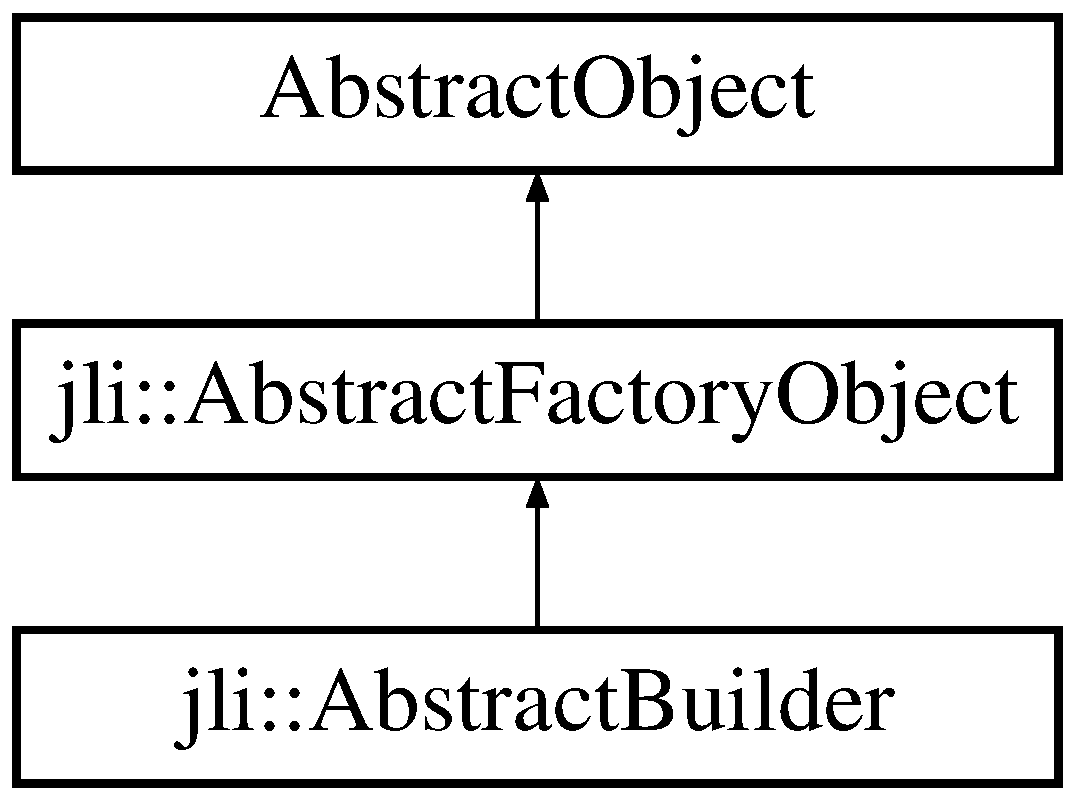
\includegraphics[height=3.000000cm]{classjli_1_1_abstract_builder}
\end{center}
\end{figure}
\subsection*{Public Member Functions}
\begin{DoxyCompactItemize}
\item 
\hyperlink{classjli_1_1_abstract_builder_a25c37208a1124c8d16688ed9627b91ac}{Abstract\+Builder} ()
\item 
\hyperlink{classjli_1_1_abstract_builder_afa72506ca991fd169f99aca02cf0a56e}{Abstract\+Builder} (const \hyperlink{classjli_1_1_abstract_builder}{Abstract\+Builder} \&)
\item 
virtual \hyperlink{classjli_1_1_abstract_builder_ac685e3eedc598acfa1f8f879e8bd8767}{$\sim$\+Abstract\+Builder} ()
\item 
\hyperlink{classjli_1_1_abstract_builder}{Abstract\+Builder} \& \hyperlink{classjli_1_1_abstract_builder_af22cd8c52e03a1ce5adad70b6b9c06cf}{operator=} (const \hyperlink{classjli_1_1_abstract_builder}{Abstract\+Builder} \&)
\item 
virtual s32 \hyperlink{classjli_1_1_abstract_builder_a107ab66007cc293eb54c74e466c5d30a}{calculate\+Serialize\+Buffer\+Size} () const =0
\item 
virtual void \hyperlink{classjli_1_1_abstract_builder_a03c8719c6b852d1a21b1c7e0b7469fc0}{serialize} (void $\ast$data\+Buffer, bt\+Serializer $\ast$serializer) const =0
\item 
virtual u32 \hyperlink{classjli_1_1_abstract_builder_ab4bc84bbd7ff6f7b14b319a9dac4f67f}{get\+Object\+Type} () const =0
\item 
virtual const char $\ast$ \hyperlink{classjli_1_1_abstract_builder_ab482a893dd560709b3ee59f27b4035f4}{get\+Class\+Name} () const =0
\item 
virtual u32 \hyperlink{classjli_1_1_abstract_builder_a826f70c995257424b7d81ab2d4706ccf}{get\+Type} () const =0
\end{DoxyCompactItemize}
\subsection*{Friends}
\begin{DoxyCompactItemize}
\item 
class \hyperlink{classjli_1_1_abstract_builder_acb96ebb09abe8f2a37a915a842babfac}{World\+Factory}
\end{DoxyCompactItemize}
\subsection*{Additional Inherited Members}


\subsection{Detailed Description}


Definition at line 20 of file Abstract\+Builder.\+h.



\subsection{Constructor \& Destructor Documentation}
\hypertarget{classjli_1_1_abstract_builder_a25c37208a1124c8d16688ed9627b91ac}{\index{jli\+::\+Abstract\+Builder@{jli\+::\+Abstract\+Builder}!Abstract\+Builder@{Abstract\+Builder}}
\index{Abstract\+Builder@{Abstract\+Builder}!jli\+::\+Abstract\+Builder@{jli\+::\+Abstract\+Builder}}
\subsubsection[{Abstract\+Builder}]{\setlength{\rightskip}{0pt plus 5cm}jli\+::\+Abstract\+Builder\+::\+Abstract\+Builder (
\begin{DoxyParamCaption}
{}
\end{DoxyParamCaption}
)}}\label{classjli_1_1_abstract_builder_a25c37208a1124c8d16688ed9627b91ac}


Definition at line 15 of file Abstract\+Builder.\+cpp.

\hypertarget{classjli_1_1_abstract_builder_afa72506ca991fd169f99aca02cf0a56e}{\index{jli\+::\+Abstract\+Builder@{jli\+::\+Abstract\+Builder}!Abstract\+Builder@{Abstract\+Builder}}
\index{Abstract\+Builder@{Abstract\+Builder}!jli\+::\+Abstract\+Builder@{jli\+::\+Abstract\+Builder}}
\subsubsection[{Abstract\+Builder}]{\setlength{\rightskip}{0pt plus 5cm}jli\+::\+Abstract\+Builder\+::\+Abstract\+Builder (
\begin{DoxyParamCaption}
\item[{const {\bf Abstract\+Builder} \&}]{copy}
\end{DoxyParamCaption}
)}}\label{classjli_1_1_abstract_builder_afa72506ca991fd169f99aca02cf0a56e}


Definition at line 21 of file Abstract\+Builder.\+cpp.

\hypertarget{classjli_1_1_abstract_builder_ac685e3eedc598acfa1f8f879e8bd8767}{\index{jli\+::\+Abstract\+Builder@{jli\+::\+Abstract\+Builder}!````~Abstract\+Builder@{$\sim$\+Abstract\+Builder}}
\index{````~Abstract\+Builder@{$\sim$\+Abstract\+Builder}!jli\+::\+Abstract\+Builder@{jli\+::\+Abstract\+Builder}}
\subsubsection[{$\sim$\+Abstract\+Builder}]{\setlength{\rightskip}{0pt plus 5cm}jli\+::\+Abstract\+Builder\+::$\sim$\+Abstract\+Builder (
\begin{DoxyParamCaption}
{}
\end{DoxyParamCaption}
)\hspace{0.3cm}{\ttfamily [virtual]}}}\label{classjli_1_1_abstract_builder_ac685e3eedc598acfa1f8f879e8bd8767}


Definition at line 27 of file Abstract\+Builder.\+cpp.



\subsection{Member Function Documentation}
\hypertarget{classjli_1_1_abstract_builder_a107ab66007cc293eb54c74e466c5d30a}{\index{jli\+::\+Abstract\+Builder@{jli\+::\+Abstract\+Builder}!calculate\+Serialize\+Buffer\+Size@{calculate\+Serialize\+Buffer\+Size}}
\index{calculate\+Serialize\+Buffer\+Size@{calculate\+Serialize\+Buffer\+Size}!jli\+::\+Abstract\+Builder@{jli\+::\+Abstract\+Builder}}
\subsubsection[{calculate\+Serialize\+Buffer\+Size}]{\setlength{\rightskip}{0pt plus 5cm}virtual s32 jli\+::\+Abstract\+Builder\+::calculate\+Serialize\+Buffer\+Size (
\begin{DoxyParamCaption}
{}
\end{DoxyParamCaption}
) const\hspace{0.3cm}{\ttfamily [pure virtual]}}}\label{classjli_1_1_abstract_builder_a107ab66007cc293eb54c74e466c5d30a}
function is used to calculate the buffer size of this object.

\begin{DoxyReturn}{Returns}
the buffer size of this object. 
\end{DoxyReturn}


Implements \hyperlink{classjli_1_1_abstract_factory_object_a37d06a25aaf9400a2f5b0a7ee110b236}{jli\+::\+Abstract\+Factory\+Object}.

\hypertarget{classjli_1_1_abstract_builder_ab482a893dd560709b3ee59f27b4035f4}{\index{jli\+::\+Abstract\+Builder@{jli\+::\+Abstract\+Builder}!get\+Class\+Name@{get\+Class\+Name}}
\index{get\+Class\+Name@{get\+Class\+Name}!jli\+::\+Abstract\+Builder@{jli\+::\+Abstract\+Builder}}
\subsubsection[{get\+Class\+Name}]{\setlength{\rightskip}{0pt plus 5cm}virtual const char$\ast$ jli\+::\+Abstract\+Builder\+::get\+Class\+Name (
\begin{DoxyParamCaption}
{}
\end{DoxyParamCaption}
) const\hspace{0.3cm}{\ttfamily [pure virtual]}}}\label{classjli_1_1_abstract_builder_ab482a893dd560709b3ee59f27b4035f4}
The name of this Class

\begin{DoxyReturn}{Returns}
the name of this class 
\end{DoxyReturn}


Implements \hyperlink{classjli_1_1_abstract_factory_object_a182551cb7d56406b4d3882fbff89a8df}{jli\+::\+Abstract\+Factory\+Object}.

\hypertarget{classjli_1_1_abstract_builder_ab4bc84bbd7ff6f7b14b319a9dac4f67f}{\index{jli\+::\+Abstract\+Builder@{jli\+::\+Abstract\+Builder}!get\+Object\+Type@{get\+Object\+Type}}
\index{get\+Object\+Type@{get\+Object\+Type}!jli\+::\+Abstract\+Builder@{jli\+::\+Abstract\+Builder}}
\subsubsection[{get\+Object\+Type}]{\setlength{\rightskip}{0pt plus 5cm}virtual u32 jli\+::\+Abstract\+Builder\+::get\+Object\+Type (
\begin{DoxyParamCaption}
{}
\end{DoxyParamCaption}
) const\hspace{0.3cm}{\ttfamily [pure virtual]}}}\label{classjli_1_1_abstract_builder_ab4bc84bbd7ff6f7b14b319a9dac4f67f}
\hypertarget{classjli_1_1_abstract_builder_a826f70c995257424b7d81ab2d4706ccf}{\index{jli\+::\+Abstract\+Builder@{jli\+::\+Abstract\+Builder}!get\+Type@{get\+Type}}
\index{get\+Type@{get\+Type}!jli\+::\+Abstract\+Builder@{jli\+::\+Abstract\+Builder}}
\subsubsection[{get\+Type}]{\setlength{\rightskip}{0pt plus 5cm}virtual u32 jli\+::\+Abstract\+Builder\+::get\+Type (
\begin{DoxyParamCaption}
{}
\end{DoxyParamCaption}
) const\hspace{0.3cm}{\ttfamily [pure virtual]}}}\label{classjli_1_1_abstract_builder_a826f70c995257424b7d81ab2d4706ccf}
The type of this Class

\begin{DoxyReturn}{Returns}
the type of this class 
\end{DoxyReturn}


Implements \hyperlink{classjli_1_1_abstract_factory_object_a7fa50dd83680e6ef5e6d3f964490a3ca}{jli\+::\+Abstract\+Factory\+Object}.

\hypertarget{classjli_1_1_abstract_builder_af22cd8c52e03a1ce5adad70b6b9c06cf}{\index{jli\+::\+Abstract\+Builder@{jli\+::\+Abstract\+Builder}!operator=@{operator=}}
\index{operator=@{operator=}!jli\+::\+Abstract\+Builder@{jli\+::\+Abstract\+Builder}}
\subsubsection[{operator=}]{\setlength{\rightskip}{0pt plus 5cm}{\bf Abstract\+Builder} \& jli\+::\+Abstract\+Builder\+::operator= (
\begin{DoxyParamCaption}
\item[{const {\bf Abstract\+Builder} \&}]{rhs}
\end{DoxyParamCaption}
)}}\label{classjli_1_1_abstract_builder_af22cd8c52e03a1ce5adad70b6b9c06cf}


Definition at line 32 of file Abstract\+Builder.\+cpp.

\hypertarget{classjli_1_1_abstract_builder_a03c8719c6b852d1a21b1c7e0b7469fc0}{\index{jli\+::\+Abstract\+Builder@{jli\+::\+Abstract\+Builder}!serialize@{serialize}}
\index{serialize@{serialize}!jli\+::\+Abstract\+Builder@{jli\+::\+Abstract\+Builder}}
\subsubsection[{serialize}]{\setlength{\rightskip}{0pt plus 5cm}virtual void jli\+::\+Abstract\+Builder\+::serialize (
\begin{DoxyParamCaption}
\item[{void $\ast$}]{data\+Buffer, }
\item[{bt\+Serializer $\ast$}]{serializer}
\end{DoxyParamCaption}
) const\hspace{0.3cm}{\ttfamily [pure virtual]}}}\label{classjli_1_1_abstract_builder_a03c8719c6b852d1a21b1c7e0b7469fc0}
Abstract function which needs to be implemented by the base class. This can be used to save the current state of the object to disk.


\begin{DoxyParams}{Parameters}
{\em data\+Buffer} & The buffer to store the data when it is finished serializing. \\
\hline
{\em serializer} & The pointer to the serializer. \\
\hline
\end{DoxyParams}


Implements \hyperlink{classjli_1_1_abstract_factory_object_a9971edc5976c06cbfae1b0ae80722a43}{jli\+::\+Abstract\+Factory\+Object}.



\subsection{Friends And Related Function Documentation}
\hypertarget{classjli_1_1_abstract_builder_acb96ebb09abe8f2a37a915a842babfac}{\index{jli\+::\+Abstract\+Builder@{jli\+::\+Abstract\+Builder}!World\+Factory@{World\+Factory}}
\index{World\+Factory@{World\+Factory}!jli\+::\+Abstract\+Builder@{jli\+::\+Abstract\+Builder}}
\subsubsection[{World\+Factory}]{\setlength{\rightskip}{0pt plus 5cm}friend class {\bf World\+Factory}\hspace{0.3cm}{\ttfamily [friend]}}}\label{classjli_1_1_abstract_builder_acb96ebb09abe8f2a37a915a842babfac}


Definition at line 23 of file Abstract\+Builder.\+h.



The documentation for this class was generated from the following files\+:\begin{DoxyCompactItemize}
\item 
\hyperlink{_abstract_builder_8h}{Abstract\+Builder.\+h}\item 
\hyperlink{_abstract_builder_8cpp}{Abstract\+Builder.\+cpp}\end{DoxyCompactItemize}

\hypertarget{classjli_1_1_node}{\section{jli\+:\+:Node Class Reference}
\label{classjli_1_1_node}\index{jli\+::\+Node@{jli\+::\+Node}}
}


{\ttfamily \#include $<$Node.\+h$>$}



Inheritance diagram for jli\+:\+:Node\+:


Collaboration diagram for jli\+:\+:Node\+:
\subsection*{Public Member Functions}
\begin{DoxyCompactItemize}
\item 
\hyperlink{classjli_1_1_node_ad3ae8427886d6e7375c62a7fb2100c4c}{Node} ()
\item 
\hyperlink{classjli_1_1_node_ac427b39c9353f0301e191f76d360d4f1}{Node} (const \hyperlink{classjli_1_1_abstract_builder}{Abstract\+Builder} \&)
\item 
\hyperlink{classjli_1_1_node_ad63185457aa77be28b780050799426f3}{Node} (const \hyperlink{classjli_1_1_node}{Node} \&)
\item 
virtual \hyperlink{classjli_1_1_node_ac46db977b2fba42d8384ccab749c9cd4}{$\sim$\+Node} ()
\item 
\hyperlink{classjli_1_1_node}{Node} \& \hyperlink{classjli_1_1_node_abbd88d2e7fcd847329cfc29f6919c40d}{operator=} (const \hyperlink{classjli_1_1_node}{Node} \&)
\item 
virtual s32 \hyperlink{classjli_1_1_node_a8075e2769a86cb0e9fa51840da53513b}{calculate\+Serialize\+Buffer\+Size} () const 
\item 
virtual void \hyperlink{classjli_1_1_node_a1dc93453f2923153cd37293bb56e6c54}{serialize} (void $\ast$, bt\+Serializer $\ast$) const 
\item 
virtual const char $\ast$ \hyperlink{classjli_1_1_node_aed60180fffdc02a1d7d598cd0595b9aa}{get\+Name} () const 
\item 
virtual u32 \hyperlink{classjli_1_1_node_a533217d7405544590a6a28fdaeec9208}{get\+Type} () const 
\end{DoxyCompactItemize}
\subsection*{Friends}
\begin{DoxyCompactItemize}
\item 
class \hyperlink{classjli_1_1_node_acb96ebb09abe8f2a37a915a842babfac}{World\+Factory}
\end{DoxyCompactItemize}


\subsection{Detailed Description}


Definition at line 17 of file Node.\+h.



\subsection{Constructor \& Destructor Documentation}
\hypertarget{classjli_1_1_node_ad3ae8427886d6e7375c62a7fb2100c4c}{\index{jli\+::\+Node@{jli\+::\+Node}!Node@{Node}}
\index{Node@{Node}!jli\+::\+Node@{jli\+::\+Node}}
\subsubsection[{Node}]{\setlength{\rightskip}{0pt plus 5cm}jli\+::\+Node\+::\+Node (
\begin{DoxyParamCaption}
{}
\end{DoxyParamCaption}
)}}\label{classjli_1_1_node_ad3ae8427886d6e7375c62a7fb2100c4c}


Definition at line 14 of file Node.\+cpp.

\hypertarget{classjli_1_1_node_ac427b39c9353f0301e191f76d360d4f1}{\index{jli\+::\+Node@{jli\+::\+Node}!Node@{Node}}
\index{Node@{Node}!jli\+::\+Node@{jli\+::\+Node}}
\subsubsection[{Node}]{\setlength{\rightskip}{0pt plus 5cm}jli\+::\+Node\+::\+Node (
\begin{DoxyParamCaption}
\item[{const {\bf Abstract\+Builder} \&}]{builder}
\end{DoxyParamCaption}
)}}\label{classjli_1_1_node_ac427b39c9353f0301e191f76d360d4f1}


Definition at line 20 of file Node.\+cpp.

\hypertarget{classjli_1_1_node_ad63185457aa77be28b780050799426f3}{\index{jli\+::\+Node@{jli\+::\+Node}!Node@{Node}}
\index{Node@{Node}!jli\+::\+Node@{jli\+::\+Node}}
\subsubsection[{Node}]{\setlength{\rightskip}{0pt plus 5cm}jli\+::\+Node\+::\+Node (
\begin{DoxyParamCaption}
\item[{const {\bf Node} \&}]{copy}
\end{DoxyParamCaption}
)}}\label{classjli_1_1_node_ad63185457aa77be28b780050799426f3}


Definition at line 26 of file Node.\+cpp.

\hypertarget{classjli_1_1_node_ac46db977b2fba42d8384ccab749c9cd4}{\index{jli\+::\+Node@{jli\+::\+Node}!````~Node@{$\sim$\+Node}}
\index{````~Node@{$\sim$\+Node}!jli\+::\+Node@{jli\+::\+Node}}
\subsubsection[{$\sim$\+Node}]{\setlength{\rightskip}{0pt plus 5cm}jli\+::\+Node\+::$\sim$\+Node (
\begin{DoxyParamCaption}
{}
\end{DoxyParamCaption}
)\hspace{0.3cm}{\ttfamily [virtual]}}}\label{classjli_1_1_node_ac46db977b2fba42d8384ccab749c9cd4}


Definition at line 32 of file Node.\+cpp.



\subsection{Member Function Documentation}
\hypertarget{classjli_1_1_node_a8075e2769a86cb0e9fa51840da53513b}{\index{jli\+::\+Node@{jli\+::\+Node}!calculate\+Serialize\+Buffer\+Size@{calculate\+Serialize\+Buffer\+Size}}
\index{calculate\+Serialize\+Buffer\+Size@{calculate\+Serialize\+Buffer\+Size}!jli\+::\+Node@{jli\+::\+Node}}
\subsubsection[{calculate\+Serialize\+Buffer\+Size}]{\setlength{\rightskip}{0pt plus 5cm}s32 jli\+::\+Node\+::calculate\+Serialize\+Buffer\+Size (
\begin{DoxyParamCaption}
{}
\end{DoxyParamCaption}
) const\hspace{0.3cm}{\ttfamily [virtual]}}}\label{classjli_1_1_node_a8075e2769a86cb0e9fa51840da53513b}


Definition at line 46 of file Node.\+cpp.

\hypertarget{classjli_1_1_node_aed60180fffdc02a1d7d598cd0595b9aa}{\index{jli\+::\+Node@{jli\+::\+Node}!get\+Name@{get\+Name}}
\index{get\+Name@{get\+Name}!jli\+::\+Node@{jli\+::\+Node}}
\subsubsection[{get\+Name}]{\setlength{\rightskip}{0pt plus 5cm}const char $\ast$ jli\+::\+Node\+::get\+Name (
\begin{DoxyParamCaption}
{}
\end{DoxyParamCaption}
) const\hspace{0.3cm}{\ttfamily [virtual]}}}\label{classjli_1_1_node_aed60180fffdc02a1d7d598cd0595b9aa}


Definition at line 57 of file Node.\+cpp.

\hypertarget{classjli_1_1_node_a533217d7405544590a6a28fdaeec9208}{\index{jli\+::\+Node@{jli\+::\+Node}!get\+Type@{get\+Type}}
\index{get\+Type@{get\+Type}!jli\+::\+Node@{jli\+::\+Node}}
\subsubsection[{get\+Type}]{\setlength{\rightskip}{0pt plus 5cm}u32 jli\+::\+Node\+::get\+Type (
\begin{DoxyParamCaption}
{}
\end{DoxyParamCaption}
) const\hspace{0.3cm}{\ttfamily [virtual]}}}\label{classjli_1_1_node_a533217d7405544590a6a28fdaeec9208}


Definition at line 62 of file Node.\+cpp.

\hypertarget{classjli_1_1_node_abbd88d2e7fcd847329cfc29f6919c40d}{\index{jli\+::\+Node@{jli\+::\+Node}!operator=@{operator=}}
\index{operator=@{operator=}!jli\+::\+Node@{jli\+::\+Node}}
\subsubsection[{operator=}]{\setlength{\rightskip}{0pt plus 5cm}{\bf Node} \& jli\+::\+Node\+::operator= (
\begin{DoxyParamCaption}
\item[{const {\bf Node} \&}]{rhs}
\end{DoxyParamCaption}
)}}\label{classjli_1_1_node_abbd88d2e7fcd847329cfc29f6919c40d}


Definition at line 37 of file Node.\+cpp.

\hypertarget{classjli_1_1_node_a1dc93453f2923153cd37293bb56e6c54}{\index{jli\+::\+Node@{jli\+::\+Node}!serialize@{serialize}}
\index{serialize@{serialize}!jli\+::\+Node@{jli\+::\+Node}}
\subsubsection[{serialize}]{\setlength{\rightskip}{0pt plus 5cm}void jli\+::\+Node\+::serialize (
\begin{DoxyParamCaption}
\item[{void $\ast$}]{data\+Buffer, }
\item[{bt\+Serializer $\ast$}]{serializer}
\end{DoxyParamCaption}
) const\hspace{0.3cm}{\ttfamily [virtual]}}}\label{classjli_1_1_node_a1dc93453f2923153cd37293bb56e6c54}


Definition at line 52 of file Node.\+cpp.



\subsection{Friends And Related Function Documentation}
\hypertarget{classjli_1_1_node_acb96ebb09abe8f2a37a915a842babfac}{\index{jli\+::\+Node@{jli\+::\+Node}!World\+Factory@{World\+Factory}}
\index{World\+Factory@{World\+Factory}!jli\+::\+Node@{jli\+::\+Node}}
\subsubsection[{World\+Factory}]{\setlength{\rightskip}{0pt plus 5cm}friend class {\bf World\+Factory}\hspace{0.3cm}{\ttfamily [friend]}}}\label{classjli_1_1_node_acb96ebb09abe8f2a37a915a842babfac}


Definition at line 20 of file Node.\+h.



The documentation for this class was generated from the following files\+:\begin{DoxyCompactItemize}
\item 
\hyperlink{_node_8h}{Node.\+h}\item 
\hyperlink{_node_8cpp}{Node.\+cpp}\end{DoxyCompactItemize}

\hypertarget{classjli_1_1_scene}{\section{jli\+:\+:Scene Class Reference}
\label{classjli_1_1_scene}\index{jli\+::\+Scene@{jli\+::\+Scene}}
}


{\ttfamily \#include $<$Scene.\+h$>$}



Inheritance diagram for jli\+:\+:Scene\+:


Collaboration diagram for jli\+:\+:Scene\+:
\subsection*{Public Member Functions}
\begin{DoxyCompactItemize}
\item 
\hyperlink{classjli_1_1_scene_abef8701bc66efaecdfb9b759f7523e9d}{Scene} ()
\item 
\hyperlink{classjli_1_1_scene_afbad74f1983633db64663db362041720}{Scene} (const \hyperlink{classjli_1_1_abstract_builder}{Abstract\+Builder} \&)
\item 
\hyperlink{classjli_1_1_scene_a4e0a2f2e6f43f3cf5e866f662dfa011a}{Scene} (const \hyperlink{classjli_1_1_scene}{Scene} \&)
\item 
virtual \hyperlink{classjli_1_1_scene_a59998f54275bafbf74434f6954f9cd2e}{$\sim$\+Scene} ()
\item 
\hyperlink{classjli_1_1_scene}{Scene} \& \hyperlink{classjli_1_1_scene_ad7e5d257a4818d182f41a82ef7347f46}{operator=} (const \hyperlink{classjli_1_1_scene}{Scene} \&)
\item 
virtual s32 \hyperlink{classjli_1_1_scene_aee7b83497bc690c184b3381f30ffd565}{calculate\+Serialize\+Buffer\+Size} () const 
\item 
virtual void \hyperlink{classjli_1_1_scene_a5cf4bf5f66daa0d35fc91eb42a9242d2}{serialize} (void $\ast$, bt\+Serializer $\ast$) const 
\item 
virtual const char $\ast$ \hyperlink{classjli_1_1_scene_a6405f60cf27b222e0d41bf161340bef7}{get\+Name} () const 
\item 
virtual u32 \hyperlink{classjli_1_1_scene_a950da1ba38b5f3973362b3225e4f3baf}{get\+Type} () const 
\end{DoxyCompactItemize}
\subsection*{Friends}
\begin{DoxyCompactItemize}
\item 
class \hyperlink{classjli_1_1_scene_acb96ebb09abe8f2a37a915a842babfac}{World\+Factory}
\end{DoxyCompactItemize}


\subsection{Detailed Description}


Definition at line 17 of file Scene.\+h.



\subsection{Constructor \& Destructor Documentation}
\hypertarget{classjli_1_1_scene_abef8701bc66efaecdfb9b759f7523e9d}{\index{jli\+::\+Scene@{jli\+::\+Scene}!Scene@{Scene}}
\index{Scene@{Scene}!jli\+::\+Scene@{jli\+::\+Scene}}
\subsubsection[{Scene}]{\setlength{\rightskip}{0pt plus 5cm}jli\+::\+Scene\+::\+Scene (
\begin{DoxyParamCaption}
{}
\end{DoxyParamCaption}
)}}\label{classjli_1_1_scene_abef8701bc66efaecdfb9b759f7523e9d}


Definition at line 14 of file Scene.\+cpp.

\hypertarget{classjli_1_1_scene_afbad74f1983633db64663db362041720}{\index{jli\+::\+Scene@{jli\+::\+Scene}!Scene@{Scene}}
\index{Scene@{Scene}!jli\+::\+Scene@{jli\+::\+Scene}}
\subsubsection[{Scene}]{\setlength{\rightskip}{0pt plus 5cm}jli\+::\+Scene\+::\+Scene (
\begin{DoxyParamCaption}
\item[{const {\bf Abstract\+Builder} \&}]{builder}
\end{DoxyParamCaption}
)}}\label{classjli_1_1_scene_afbad74f1983633db64663db362041720}


Definition at line 20 of file Scene.\+cpp.

\hypertarget{classjli_1_1_scene_a4e0a2f2e6f43f3cf5e866f662dfa011a}{\index{jli\+::\+Scene@{jli\+::\+Scene}!Scene@{Scene}}
\index{Scene@{Scene}!jli\+::\+Scene@{jli\+::\+Scene}}
\subsubsection[{Scene}]{\setlength{\rightskip}{0pt plus 5cm}jli\+::\+Scene\+::\+Scene (
\begin{DoxyParamCaption}
\item[{const {\bf Scene} \&}]{copy}
\end{DoxyParamCaption}
)}}\label{classjli_1_1_scene_a4e0a2f2e6f43f3cf5e866f662dfa011a}


Definition at line 26 of file Scene.\+cpp.

\hypertarget{classjli_1_1_scene_a59998f54275bafbf74434f6954f9cd2e}{\index{jli\+::\+Scene@{jli\+::\+Scene}!````~Scene@{$\sim$\+Scene}}
\index{````~Scene@{$\sim$\+Scene}!jli\+::\+Scene@{jli\+::\+Scene}}
\subsubsection[{$\sim$\+Scene}]{\setlength{\rightskip}{0pt plus 5cm}jli\+::\+Scene\+::$\sim$\+Scene (
\begin{DoxyParamCaption}
{}
\end{DoxyParamCaption}
)\hspace{0.3cm}{\ttfamily [virtual]}}}\label{classjli_1_1_scene_a59998f54275bafbf74434f6954f9cd2e}


Definition at line 32 of file Scene.\+cpp.



\subsection{Member Function Documentation}
\hypertarget{classjli_1_1_scene_aee7b83497bc690c184b3381f30ffd565}{\index{jli\+::\+Scene@{jli\+::\+Scene}!calculate\+Serialize\+Buffer\+Size@{calculate\+Serialize\+Buffer\+Size}}
\index{calculate\+Serialize\+Buffer\+Size@{calculate\+Serialize\+Buffer\+Size}!jli\+::\+Scene@{jli\+::\+Scene}}
\subsubsection[{calculate\+Serialize\+Buffer\+Size}]{\setlength{\rightskip}{0pt plus 5cm}s32 jli\+::\+Scene\+::calculate\+Serialize\+Buffer\+Size (
\begin{DoxyParamCaption}
{}
\end{DoxyParamCaption}
) const\hspace{0.3cm}{\ttfamily [virtual]}}}\label{classjli_1_1_scene_aee7b83497bc690c184b3381f30ffd565}


Definition at line 46 of file Scene.\+cpp.

\hypertarget{classjli_1_1_scene_a6405f60cf27b222e0d41bf161340bef7}{\index{jli\+::\+Scene@{jli\+::\+Scene}!get\+Name@{get\+Name}}
\index{get\+Name@{get\+Name}!jli\+::\+Scene@{jli\+::\+Scene}}
\subsubsection[{get\+Name}]{\setlength{\rightskip}{0pt plus 5cm}const char $\ast$ jli\+::\+Scene\+::get\+Name (
\begin{DoxyParamCaption}
{}
\end{DoxyParamCaption}
) const\hspace{0.3cm}{\ttfamily [virtual]}}}\label{classjli_1_1_scene_a6405f60cf27b222e0d41bf161340bef7}


Definition at line 57 of file Scene.\+cpp.

\hypertarget{classjli_1_1_scene_a950da1ba38b5f3973362b3225e4f3baf}{\index{jli\+::\+Scene@{jli\+::\+Scene}!get\+Type@{get\+Type}}
\index{get\+Type@{get\+Type}!jli\+::\+Scene@{jli\+::\+Scene}}
\subsubsection[{get\+Type}]{\setlength{\rightskip}{0pt plus 5cm}u32 jli\+::\+Scene\+::get\+Type (
\begin{DoxyParamCaption}
{}
\end{DoxyParamCaption}
) const\hspace{0.3cm}{\ttfamily [virtual]}}}\label{classjli_1_1_scene_a950da1ba38b5f3973362b3225e4f3baf}


Definition at line 62 of file Scene.\+cpp.

\hypertarget{classjli_1_1_scene_ad7e5d257a4818d182f41a82ef7347f46}{\index{jli\+::\+Scene@{jli\+::\+Scene}!operator=@{operator=}}
\index{operator=@{operator=}!jli\+::\+Scene@{jli\+::\+Scene}}
\subsubsection[{operator=}]{\setlength{\rightskip}{0pt plus 5cm}{\bf Scene} \& jli\+::\+Scene\+::operator= (
\begin{DoxyParamCaption}
\item[{const {\bf Scene} \&}]{rhs}
\end{DoxyParamCaption}
)}}\label{classjli_1_1_scene_ad7e5d257a4818d182f41a82ef7347f46}


Definition at line 37 of file Scene.\+cpp.

\hypertarget{classjli_1_1_scene_a5cf4bf5f66daa0d35fc91eb42a9242d2}{\index{jli\+::\+Scene@{jli\+::\+Scene}!serialize@{serialize}}
\index{serialize@{serialize}!jli\+::\+Scene@{jli\+::\+Scene}}
\subsubsection[{serialize}]{\setlength{\rightskip}{0pt plus 5cm}void jli\+::\+Scene\+::serialize (
\begin{DoxyParamCaption}
\item[{void $\ast$}]{data\+Buffer, }
\item[{bt\+Serializer $\ast$}]{serializer}
\end{DoxyParamCaption}
) const\hspace{0.3cm}{\ttfamily [virtual]}}}\label{classjli_1_1_scene_a5cf4bf5f66daa0d35fc91eb42a9242d2}


Definition at line 52 of file Scene.\+cpp.



\subsection{Friends And Related Function Documentation}
\hypertarget{classjli_1_1_scene_acb96ebb09abe8f2a37a915a842babfac}{\index{jli\+::\+Scene@{jli\+::\+Scene}!World\+Factory@{World\+Factory}}
\index{World\+Factory@{World\+Factory}!jli\+::\+Scene@{jli\+::\+Scene}}
\subsubsection[{World\+Factory}]{\setlength{\rightskip}{0pt plus 5cm}friend class {\bf World\+Factory}\hspace{0.3cm}{\ttfamily [friend]}}}\label{classjli_1_1_scene_acb96ebb09abe8f2a37a915a842babfac}


Definition at line 20 of file Scene.\+h.



The documentation for this class was generated from the following files\+:\begin{DoxyCompactItemize}
\item 
\hyperlink{_scene_8h}{Scene.\+h}\item 
\hyperlink{_scene_8cpp}{Scene.\+cpp}\end{DoxyCompactItemize}

\hypertarget{classjli_1_1_world}{\section{jli\+:\+:World Class Reference}
\label{classjli_1_1_world}\index{jli\+::\+World@{jli\+::\+World}}
}


{\ttfamily \#include $<$World.\+h$>$}

\subsection*{Public Member Functions}
\begin{DoxyCompactItemize}
\item 
\hyperlink{classjli_1_1_world_ab340b6a4f69503333397ec65b091414a}{World} ()
\item 
virtual \hyperlink{classjli_1_1_world_a23e1f8b843020bdcec4b3ece3a89d1b8}{$\sim$\+World} ()
\item 
\hyperlink{classjli_1_1_world_factory}{World\+Factory} $\ast$const \hyperlink{classjli_1_1_world_aef4b78708b5daf80703d8a57f2b0f5ae}{get\+World\+Factory} () const 
\item 
\hyperlink{classjli_1_1_world_my_s_q_l}{World\+My\+S\+Q\+L} $\ast$const \hyperlink{classjli_1_1_world_ae8b75d8993a718753d589d49f2c00094}{get\+World\+My\+S\+Q\+L} () const 
\item 
\hyperlink{classjli_1_1_world_input}{World\+Input} $\ast$const \hyperlink{classjli_1_1_world_aeee764fef2643e963d08df7c891f4a26}{get\+World\+Input} () const 
\item 
\hyperlink{classjli_1_1_world_sound}{World\+Sound} $\ast$const \hyperlink{classjli_1_1_world_a00a7fc82c5723b567fa118e029712d34}{get\+World\+Sound} () const 
\item 
\hyperlink{classjli_1_1_world_lua_virtual_machine}{World\+Lua\+Virtual\+Machine} $\ast$const \hyperlink{classjli_1_1_world_a4a11fef67cef6d596344a5f5db79b4fb}{get\+World\+Lua\+Virtual\+Machine} () const 
\item 
\hyperlink{namespacejli_af69056b00744493ba074ef13e82b0bec}{Clock} $\ast$const \hyperlink{classjli_1_1_world_a4e35bb1d091a72f667de5c4cbc6e04b8}{get\+World\+Clock} () const 
\end{DoxyCompactItemize}
\subsection*{Static Public Member Functions}
\begin{DoxyCompactItemize}
\item 
static void \hyperlink{classjli_1_1_world_af250acadd5336ddfebbff7c934c4d410}{create\+Instance} ()
\item 
static void \hyperlink{classjli_1_1_world_afbf269b5621c765b5eadbdfc0bbc7457}{destroy\+Instance} ()
\item 
static \hyperlink{classjli_1_1_world}{World} $\ast$const \hyperlink{classjli_1_1_world_a206e13757c28b84d9739b052a2e37e99}{get\+Instance} ()
\item 
static bool \hyperlink{classjli_1_1_world_a730a4745d8a020a240d8445761ab69a8}{has\+Instance} ()
\end{DoxyCompactItemize}


\subsection{Detailed Description}


Definition at line 24 of file World.\+h.



\subsection{Constructor \& Destructor Documentation}
\hypertarget{classjli_1_1_world_ab340b6a4f69503333397ec65b091414a}{\index{jli\+::\+World@{jli\+::\+World}!World@{World}}
\index{World@{World}!jli\+::\+World@{jli\+::\+World}}
\subsubsection[{World}]{\setlength{\rightskip}{0pt plus 5cm}jli\+::\+World\+::\+World (
\begin{DoxyParamCaption}
{}
\end{DoxyParamCaption}
)}}\label{classjli_1_1_world_ab340b6a4f69503333397ec65b091414a}


Definition at line 41 of file World.\+cpp.

\hypertarget{classjli_1_1_world_a23e1f8b843020bdcec4b3ece3a89d1b8}{\index{jli\+::\+World@{jli\+::\+World}!````~World@{$\sim$\+World}}
\index{````~World@{$\sim$\+World}!jli\+::\+World@{jli\+::\+World}}
\subsubsection[{$\sim$\+World}]{\setlength{\rightskip}{0pt plus 5cm}jli\+::\+World\+::$\sim$\+World (
\begin{DoxyParamCaption}
{}
\end{DoxyParamCaption}
)\hspace{0.3cm}{\ttfamily [virtual]}}}\label{classjli_1_1_world_a23e1f8b843020bdcec4b3ece3a89d1b8}


Definition at line 51 of file World.\+cpp.



\subsection{Member Function Documentation}
\hypertarget{classjli_1_1_world_af250acadd5336ddfebbff7c934c4d410}{\index{jli\+::\+World@{jli\+::\+World}!create\+Instance@{create\+Instance}}
\index{create\+Instance@{create\+Instance}!jli\+::\+World@{jli\+::\+World}}
\subsubsection[{create\+Instance}]{\setlength{\rightskip}{0pt plus 5cm}void jli\+::\+World\+::create\+Instance (
\begin{DoxyParamCaption}
{}
\end{DoxyParamCaption}
)\hspace{0.3cm}{\ttfamily [static]}}}\label{classjli_1_1_world_af250acadd5336ddfebbff7c934c4d410}


Definition at line 15 of file World.\+cpp.

\hypertarget{classjli_1_1_world_afbf269b5621c765b5eadbdfc0bbc7457}{\index{jli\+::\+World@{jli\+::\+World}!destroy\+Instance@{destroy\+Instance}}
\index{destroy\+Instance@{destroy\+Instance}!jli\+::\+World@{jli\+::\+World}}
\subsubsection[{destroy\+Instance}]{\setlength{\rightskip}{0pt plus 5cm}void jli\+::\+World\+::destroy\+Instance (
\begin{DoxyParamCaption}
{}
\end{DoxyParamCaption}
)\hspace{0.3cm}{\ttfamily [static]}}}\label{classjli_1_1_world_afbf269b5621c765b5eadbdfc0bbc7457}


Definition at line 23 of file World.\+cpp.

\hypertarget{classjli_1_1_world_a206e13757c28b84d9739b052a2e37e99}{\index{jli\+::\+World@{jli\+::\+World}!get\+Instance@{get\+Instance}}
\index{get\+Instance@{get\+Instance}!jli\+::\+World@{jli\+::\+World}}
\subsubsection[{get\+Instance}]{\setlength{\rightskip}{0pt plus 5cm}{\bf World} $\ast$const jli\+::\+World\+::get\+Instance (
\begin{DoxyParamCaption}
{}
\end{DoxyParamCaption}
)\hspace{0.3cm}{\ttfamily [static]}}}\label{classjli_1_1_world_a206e13757c28b84d9739b052a2e37e99}


Definition at line 29 of file World.\+cpp.

\hypertarget{classjli_1_1_world_a4e35bb1d091a72f667de5c4cbc6e04b8}{\index{jli\+::\+World@{jli\+::\+World}!get\+World\+Clock@{get\+World\+Clock}}
\index{get\+World\+Clock@{get\+World\+Clock}!jli\+::\+World@{jli\+::\+World}}
\subsubsection[{get\+World\+Clock}]{\setlength{\rightskip}{0pt plus 5cm}{\bf Clock} $\ast$const jli\+::\+World\+::get\+World\+Clock (
\begin{DoxyParamCaption}
{}
\end{DoxyParamCaption}
) const}}\label{classjli_1_1_world_a4e35bb1d091a72f667de5c4cbc6e04b8}


Definition at line 86 of file World.\+cpp.

\hypertarget{classjli_1_1_world_aef4b78708b5daf80703d8a57f2b0f5ae}{\index{jli\+::\+World@{jli\+::\+World}!get\+World\+Factory@{get\+World\+Factory}}
\index{get\+World\+Factory@{get\+World\+Factory}!jli\+::\+World@{jli\+::\+World}}
\subsubsection[{get\+World\+Factory}]{\setlength{\rightskip}{0pt plus 5cm}{\bf World\+Factory} $\ast$const jli\+::\+World\+::get\+World\+Factory (
\begin{DoxyParamCaption}
{}
\end{DoxyParamCaption}
) const}}\label{classjli_1_1_world_aef4b78708b5daf80703d8a57f2b0f5ae}


Definition at line 61 of file World.\+cpp.

\hypertarget{classjli_1_1_world_aeee764fef2643e963d08df7c891f4a26}{\index{jli\+::\+World@{jli\+::\+World}!get\+World\+Input@{get\+World\+Input}}
\index{get\+World\+Input@{get\+World\+Input}!jli\+::\+World@{jli\+::\+World}}
\subsubsection[{get\+World\+Input}]{\setlength{\rightskip}{0pt plus 5cm}{\bf World\+Input} $\ast$const jli\+::\+World\+::get\+World\+Input (
\begin{DoxyParamCaption}
{}
\end{DoxyParamCaption}
) const}}\label{classjli_1_1_world_aeee764fef2643e963d08df7c891f4a26}


Definition at line 71 of file World.\+cpp.

\hypertarget{classjli_1_1_world_a4a11fef67cef6d596344a5f5db79b4fb}{\index{jli\+::\+World@{jli\+::\+World}!get\+World\+Lua\+Virtual\+Machine@{get\+World\+Lua\+Virtual\+Machine}}
\index{get\+World\+Lua\+Virtual\+Machine@{get\+World\+Lua\+Virtual\+Machine}!jli\+::\+World@{jli\+::\+World}}
\subsubsection[{get\+World\+Lua\+Virtual\+Machine}]{\setlength{\rightskip}{0pt plus 5cm}{\bf World\+Lua\+Virtual\+Machine} $\ast$const jli\+::\+World\+::get\+World\+Lua\+Virtual\+Machine (
\begin{DoxyParamCaption}
{}
\end{DoxyParamCaption}
) const}}\label{classjli_1_1_world_a4a11fef67cef6d596344a5f5db79b4fb}


Definition at line 81 of file World.\+cpp.

\hypertarget{classjli_1_1_world_ae8b75d8993a718753d589d49f2c00094}{\index{jli\+::\+World@{jli\+::\+World}!get\+World\+My\+S\+Q\+L@{get\+World\+My\+S\+Q\+L}}
\index{get\+World\+My\+S\+Q\+L@{get\+World\+My\+S\+Q\+L}!jli\+::\+World@{jli\+::\+World}}
\subsubsection[{get\+World\+My\+S\+Q\+L}]{\setlength{\rightskip}{0pt plus 5cm}{\bf World\+My\+S\+Q\+L} $\ast$const jli\+::\+World\+::get\+World\+My\+S\+Q\+L (
\begin{DoxyParamCaption}
{}
\end{DoxyParamCaption}
) const}}\label{classjli_1_1_world_ae8b75d8993a718753d589d49f2c00094}


Definition at line 66 of file World.\+cpp.

\hypertarget{classjli_1_1_world_a00a7fc82c5723b567fa118e029712d34}{\index{jli\+::\+World@{jli\+::\+World}!get\+World\+Sound@{get\+World\+Sound}}
\index{get\+World\+Sound@{get\+World\+Sound}!jli\+::\+World@{jli\+::\+World}}
\subsubsection[{get\+World\+Sound}]{\setlength{\rightskip}{0pt plus 5cm}{\bf World\+Sound} $\ast$const jli\+::\+World\+::get\+World\+Sound (
\begin{DoxyParamCaption}
{}
\end{DoxyParamCaption}
) const}}\label{classjli_1_1_world_a00a7fc82c5723b567fa118e029712d34}


Definition at line 76 of file World.\+cpp.

\hypertarget{classjli_1_1_world_a730a4745d8a020a240d8445761ab69a8}{\index{jli\+::\+World@{jli\+::\+World}!has\+Instance@{has\+Instance}}
\index{has\+Instance@{has\+Instance}!jli\+::\+World@{jli\+::\+World}}
\subsubsection[{has\+Instance}]{\setlength{\rightskip}{0pt plus 5cm}bool jli\+::\+World\+::has\+Instance (
\begin{DoxyParamCaption}
{}
\end{DoxyParamCaption}
)\hspace{0.3cm}{\ttfamily [static]}}}\label{classjli_1_1_world_a730a4745d8a020a240d8445761ab69a8}


Definition at line 36 of file World.\+cpp.



The documentation for this class was generated from the following files\+:\begin{DoxyCompactItemize}
\item 
/\+Users/jamesfolk/\+Dropbox/\+Game\+Development/mygames/third\+\_\+party/jli\+\_\+game\+\_\+engine/src/\hyperlink{_world_8h}{World.\+h}\item 
/\+Users/jamesfolk/\+Dropbox/\+Game\+Development/mygames/third\+\_\+party/jli\+\_\+game\+\_\+engine/src/\hyperlink{_world_8cpp}{World.\+cpp}\end{DoxyCompactItemize}

\hypertarget{classjli_1_1_world_factory}{\section{jli\+:\+:World\+Factory Class Reference}
\label{classjli_1_1_world_factory}\index{jli\+::\+World\+Factory@{jli\+::\+World\+Factory}}
}


{\ttfamily \#include $<$World\+Factory.\+h$>$}

\subsection*{Public Types}
\begin{DoxyCompactItemize}
\item 
typedef bt\+Aligned\+Object\+Array\\*
$<$ \hyperlink{classjli_1_1_abstract_factory_object}{Abstract\+Factory\+Object} $\ast$ $>$ \hyperlink{classjli_1_1_world_factory_ab7d8f835ed36ede3da410326c80709c8}{Object\+List}
\item 
typedef bt\+Hash\+Map$<$ bt\+Hash\+Ptr, s32 $>$ \hyperlink{classjli_1_1_world_factory_ac26bf6a5e096985680e8a45b33f7873c}{Object\+Duplicate\+Map}
\end{DoxyCompactItemize}
\subsection*{Public Member Functions}
\begin{DoxyCompactItemize}
\item 
virtual \hyperlink{classjli_1_1_abstract_factory_object}{Abstract\+Factory\+Object} $\ast$ \hyperlink{classjli_1_1_world_factory_ae84dad80ebffaf34cdc7fe95d1e7a66e}{create} (const u32 type)
\item 
virtual \hyperlink{classjli_1_1_abstract_factory_object}{Abstract\+Factory\+Object} $\ast$ \hyperlink{classjli_1_1_world_factory_a7907b82e19f4bbb1f5c98fbceaf7d961}{create} (const \hyperlink{classjli_1_1_abstract_builder}{Abstract\+Builder} \&)
\item 
virtual \hyperlink{classjli_1_1_abstract_factory_object}{Abstract\+Factory\+Object} $\ast$ \hyperlink{classjli_1_1_world_factory_aadc177f52ddc2a0d53259ea99fbf90df}{clone} (const \hyperlink{classjli_1_1_abstract_factory_object}{Abstract\+Factory\+Object} \&, bool=false)
\item 
virtual bool \hyperlink{classjli_1_1_world_factory_a29af5f1c2a8f5e57c0dc4e9764715797}{has} (\hyperlink{classjli_1_1_abstract_factory_object}{Abstract\+Factory\+Object} $\ast$) const 
\item 
virtual void \hyperlink{classjli_1_1_world_factory_a715756195f93bfec6f6c54640e5e09e5}{destroy\+Instance} (\hyperlink{classjli_1_1_abstract_factory_object}{Abstract\+Factory\+Object} $\ast$)
\item 
virtual void \hyperlink{classjli_1_1_world_factory_ac40ef526c98ded68e2be556995147ca5}{destroy} (\hyperlink{classjli_1_1_abstract_factory_object}{Abstract\+Factory\+Object} $\ast$)
\item 
virtual void \hyperlink{classjli_1_1_world_factory_a17880329ad38799467c11830c8b2b39e}{destroy\+All} ()
\item 
virtual s32 \hyperlink{classjli_1_1_world_factory_a56279adb8ce6f7072739a5b7eeccd45b}{size} ()
\item 
virtual s32 \hyperlink{classjli_1_1_world_factory_a6305d49494b83a45f77c4065efe595d3}{instances} (const u32)
\item 
virtual s32 \hyperlink{classjli_1_1_world_factory_a352be79efeb80d15cf9e7c9cafc8d47a}{instances} (\hyperlink{classjli_1_1_abstract_factory_object}{Abstract\+Factory\+Object} $\ast$)
\item 
virtual \hyperlink{classjli_1_1_abstract_factory_object}{Abstract\+Factory\+Object} $\ast$ \hyperlink{classjli_1_1_world_factory_a44235d0cb9e7e11fa7df8b2c7c84e77b}{get} (const u32) const 
\item 
virtual void \hyperlink{classjli_1_1_world_factory_afc3c3ab16e547f8efb70df6c0a6c9acc}{get\+All} (bt\+Aligned\+Object\+Array$<$ \hyperlink{classjli_1_1_abstract_factory_object}{Abstract\+Factory\+Object} $\ast$ $>$ \&) const 
\item 
virtual s32 \hyperlink{classjli_1_1_world_factory_a36ed5d3e23a486003b5490dbd117c308}{index} (\hyperlink{classjli_1_1_abstract_factory_object}{Abstract\+Factory\+Object} $\ast$) const 
\item 
virtual void \hyperlink{classjli_1_1_world_factory_a4cb7bc0a2b06508944575416716a2630}{serialize} (bt\+Serializer $\ast$serializer)
\item 
\hyperlink{classjli_1_1_world_factory_aa0743bb8d687c225a725d68360c84cee}{World\+Factory} ()
\item 
virtual \hyperlink{classjli_1_1_world_factory_ab07df554e2f6d0777470dc426020ceeb}{$\sim$\+World\+Factory} ()
\item 
virtual \hyperlink{classjli_1_1_abstract_factory_object}{Abstract\+Factory\+Object} $\ast$ \hyperlink{classjli_1_1_world_factory_a1651da687bf991ffafa8f02bc3eb9707}{ctor} (const u32 \&)
\item 
virtual \hyperlink{classjli_1_1_abstract_factory_object}{Abstract\+Factory\+Object} $\ast$ \hyperlink{classjli_1_1_world_factory_a0b8a82380ee533205802acb2c58af331}{ctor} (const \hyperlink{classjli_1_1_abstract_builder}{jli\+::\+Abstract\+Builder} \&)
\item 
virtual \hyperlink{classjli_1_1_abstract_factory_object}{Abstract\+Factory\+Object} $\ast$ \hyperlink{classjli_1_1_world_factory_a62f73f5ea8689adf2652de1111f05915}{ctor} (const \hyperlink{classjli_1_1_abstract_factory_object}{Abstract\+Factory\+Object} \&)
\item 
\hyperlink{classjli_1_1_abstract_factory_object}{Abstract\+Factory\+Object} $\ast$ \hyperlink{classjli_1_1_world_factory_a950011f467778776bffd2fe0a149293a}{create\+\_\+\+Internal} (const u32)
\item 
\hyperlink{classjli_1_1_abstract_factory_object}{Abstract\+Factory\+Object} $\ast$ \hyperlink{classjli_1_1_world_factory_a0bbb3e37df86e691253179a12bdc191d}{create\+\_\+\+Internal} (const \hyperlink{classjli_1_1_abstract_builder}{Abstract\+Builder} \&)
\item 
\hyperlink{classjli_1_1_abstract_factory_object}{Abstract\+Factory\+Object} $\ast$ \hyperlink{classjli_1_1_world_factory_aa0f13c33f5e308f48ef1db874bc897fb}{clone\+\_\+\+Internal} (const \hyperlink{classjli_1_1_abstract_factory_object}{Abstract\+Factory\+Object} \&, bool)
\item 
void \hyperlink{classjli_1_1_world_factory_ac3348faaa06a437c9bdff93f0245d1e1}{remove\+\_\+\+Internal} (\hyperlink{classjli_1_1_abstract_factory_object}{Abstract\+Factory\+Object} $\ast$)
\end{DoxyCompactItemize}
\subsection*{Public Attributes}
\begin{DoxyCompactItemize}
\item 
\hyperlink{classjli_1_1_world_factory_ab7d8f835ed36ede3da410326c80709c8}{Object\+List} \hyperlink{classjli_1_1_world_factory_ac1a42314be66db6555d7723a35d2cdbc}{m\+\_\+\+Object\+List}
\item 
\hyperlink{classjli_1_1_world_factory_ac26bf6a5e096985680e8a45b33f7873c}{Object\+Duplicate\+Map} \hyperlink{classjli_1_1_world_factory_a67d271ea8de7eaee463069a9e3e46f4e}{m\+\_\+\+Object\+Duplicate\+Map}
\end{DoxyCompactItemize}


\subsection{Detailed Description}


Definition at line 94 of file World\+Factory.\+h.



\subsection{Member Typedef Documentation}
\hypertarget{classjli_1_1_world_factory_ac26bf6a5e096985680e8a45b33f7873c}{\index{jli\+::\+World\+Factory@{jli\+::\+World\+Factory}!Object\+Duplicate\+Map@{Object\+Duplicate\+Map}}
\index{Object\+Duplicate\+Map@{Object\+Duplicate\+Map}!jli\+::\+World\+Factory@{jli\+::\+World\+Factory}}
\subsubsection[{Object\+Duplicate\+Map}]{\setlength{\rightskip}{0pt plus 5cm}typedef bt\+Hash\+Map$<$bt\+Hash\+Ptr, s32$>$ {\bf jli\+::\+World\+Factory\+::\+Object\+Duplicate\+Map}}}\label{classjli_1_1_world_factory_ac26bf6a5e096985680e8a45b33f7873c}


Definition at line 98 of file World\+Factory.\+h.

\hypertarget{classjli_1_1_world_factory_ab7d8f835ed36ede3da410326c80709c8}{\index{jli\+::\+World\+Factory@{jli\+::\+World\+Factory}!Object\+List@{Object\+List}}
\index{Object\+List@{Object\+List}!jli\+::\+World\+Factory@{jli\+::\+World\+Factory}}
\subsubsection[{Object\+List}]{\setlength{\rightskip}{0pt plus 5cm}typedef bt\+Aligned\+Object\+Array$<${\bf Abstract\+Factory\+Object}$\ast$$>$ {\bf jli\+::\+World\+Factory\+::\+Object\+List}}}\label{classjli_1_1_world_factory_ab7d8f835ed36ede3da410326c80709c8}


Definition at line 97 of file World\+Factory.\+h.



\subsection{Constructor \& Destructor Documentation}
\hypertarget{classjli_1_1_world_factory_aa0743bb8d687c225a725d68360c84cee}{\index{jli\+::\+World\+Factory@{jli\+::\+World\+Factory}!World\+Factory@{World\+Factory}}
\index{World\+Factory@{World\+Factory}!jli\+::\+World\+Factory@{jli\+::\+World\+Factory}}
\subsubsection[{World\+Factory}]{\setlength{\rightskip}{0pt plus 5cm}jli\+::\+World\+Factory\+::\+World\+Factory (
\begin{DoxyParamCaption}
{}
\end{DoxyParamCaption}
)}}\label{classjli_1_1_world_factory_aa0743bb8d687c225a725d68360c84cee}


Definition at line 186 of file World\+Factory.\+cpp.

\hypertarget{classjli_1_1_world_factory_ab07df554e2f6d0777470dc426020ceeb}{\index{jli\+::\+World\+Factory@{jli\+::\+World\+Factory}!````~World\+Factory@{$\sim$\+World\+Factory}}
\index{````~World\+Factory@{$\sim$\+World\+Factory}!jli\+::\+World\+Factory@{jli\+::\+World\+Factory}}
\subsubsection[{$\sim$\+World\+Factory}]{\setlength{\rightskip}{0pt plus 5cm}jli\+::\+World\+Factory\+::$\sim$\+World\+Factory (
\begin{DoxyParamCaption}
{}
\end{DoxyParamCaption}
)\hspace{0.3cm}{\ttfamily [virtual]}}}\label{classjli_1_1_world_factory_ab07df554e2f6d0777470dc426020ceeb}


Definition at line 191 of file World\+Factory.\+cpp.



\subsection{Member Function Documentation}
\hypertarget{classjli_1_1_world_factory_aadc177f52ddc2a0d53259ea99fbf90df}{\index{jli\+::\+World\+Factory@{jli\+::\+World\+Factory}!clone@{clone}}
\index{clone@{clone}!jli\+::\+World\+Factory@{jli\+::\+World\+Factory}}
\subsubsection[{clone}]{\setlength{\rightskip}{0pt plus 5cm}{\bf Abstract\+Factory\+Object} $\ast$ jli\+::\+World\+Factory\+::clone (
\begin{DoxyParamCaption}
\item[{const {\bf Abstract\+Factory\+Object} \&}]{object, }
\item[{bool}]{share = {\ttfamily false}}
\end{DoxyParamCaption}
)\hspace{0.3cm}{\ttfamily [virtual]}}}\label{classjli_1_1_world_factory_aadc177f52ddc2a0d53259ea99fbf90df}


Definition at line 87 of file World\+Factory.\+cpp.

\hypertarget{classjli_1_1_world_factory_aa0f13c33f5e308f48ef1db874bc897fb}{\index{jli\+::\+World\+Factory@{jli\+::\+World\+Factory}!clone\+\_\+\+Internal@{clone\+\_\+\+Internal}}
\index{clone\+\_\+\+Internal@{clone\+\_\+\+Internal}!jli\+::\+World\+Factory@{jli\+::\+World\+Factory}}
\subsubsection[{clone\+\_\+\+Internal}]{\setlength{\rightskip}{0pt plus 5cm}{\bf Abstract\+Factory\+Object} $\ast$ jli\+::\+World\+Factory\+::clone\+\_\+\+Internal (
\begin{DoxyParamCaption}
\item[{const {\bf Abstract\+Factory\+Object} \&}]{copy, }
\item[{bool}]{share}
\end{DoxyParamCaption}
)}}\label{classjli_1_1_world_factory_aa0f13c33f5e308f48ef1db874bc897fb}


Definition at line 752 of file World\+Factory.\+cpp.

\hypertarget{classjli_1_1_world_factory_ae84dad80ebffaf34cdc7fe95d1e7a66e}{\index{jli\+::\+World\+Factory@{jli\+::\+World\+Factory}!create@{create}}
\index{create@{create}!jli\+::\+World\+Factory@{jli\+::\+World\+Factory}}
\subsubsection[{create}]{\setlength{\rightskip}{0pt plus 5cm}{\bf Abstract\+Factory\+Object} $\ast$ jli\+::\+World\+Factory\+::create (
\begin{DoxyParamCaption}
\item[{const u32}]{type}
\end{DoxyParamCaption}
)\hspace{0.3cm}{\ttfamily [virtual]}}}\label{classjli_1_1_world_factory_ae84dad80ebffaf34cdc7fe95d1e7a66e}


Definition at line 78 of file World\+Factory.\+cpp.

\hypertarget{classjli_1_1_world_factory_a7907b82e19f4bbb1f5c98fbceaf7d961}{\index{jli\+::\+World\+Factory@{jli\+::\+World\+Factory}!create@{create}}
\index{create@{create}!jli\+::\+World\+Factory@{jli\+::\+World\+Factory}}
\subsubsection[{create}]{\setlength{\rightskip}{0pt plus 5cm}{\bf Abstract\+Factory\+Object} $\ast$ jli\+::\+World\+Factory\+::create (
\begin{DoxyParamCaption}
\item[{const {\bf Abstract\+Builder} \&}]{builder}
\end{DoxyParamCaption}
)\hspace{0.3cm}{\ttfamily [virtual]}}}\label{classjli_1_1_world_factory_a7907b82e19f4bbb1f5c98fbceaf7d961}


Definition at line 82 of file World\+Factory.\+cpp.

\hypertarget{classjli_1_1_world_factory_a950011f467778776bffd2fe0a149293a}{\index{jli\+::\+World\+Factory@{jli\+::\+World\+Factory}!create\+\_\+\+Internal@{create\+\_\+\+Internal}}
\index{create\+\_\+\+Internal@{create\+\_\+\+Internal}!jli\+::\+World\+Factory@{jli\+::\+World\+Factory}}
\subsubsection[{create\+\_\+\+Internal}]{\setlength{\rightskip}{0pt plus 5cm}{\bf Abstract\+Factory\+Object} $\ast$ jli\+::\+World\+Factory\+::create\+\_\+\+Internal (
\begin{DoxyParamCaption}
\item[{const u32}]{type}
\end{DoxyParamCaption}
)}}\label{classjli_1_1_world_factory_a950011f467778776bffd2fe0a149293a}


Definition at line 725 of file World\+Factory.\+cpp.

\hypertarget{classjli_1_1_world_factory_a0bbb3e37df86e691253179a12bdc191d}{\index{jli\+::\+World\+Factory@{jli\+::\+World\+Factory}!create\+\_\+\+Internal@{create\+\_\+\+Internal}}
\index{create\+\_\+\+Internal@{create\+\_\+\+Internal}!jli\+::\+World\+Factory@{jli\+::\+World\+Factory}}
\subsubsection[{create\+\_\+\+Internal}]{\setlength{\rightskip}{0pt plus 5cm}{\bf Abstract\+Factory\+Object} $\ast$ jli\+::\+World\+Factory\+::create\+\_\+\+Internal (
\begin{DoxyParamCaption}
\item[{const {\bf Abstract\+Builder} \&}]{builder}
\end{DoxyParamCaption}
)}}\label{classjli_1_1_world_factory_a0bbb3e37df86e691253179a12bdc191d}


Definition at line 738 of file World\+Factory.\+cpp.

\hypertarget{classjli_1_1_world_factory_a1651da687bf991ffafa8f02bc3eb9707}{\index{jli\+::\+World\+Factory@{jli\+::\+World\+Factory}!ctor@{ctor}}
\index{ctor@{ctor}!jli\+::\+World\+Factory@{jli\+::\+World\+Factory}}
\subsubsection[{ctor}]{\setlength{\rightskip}{0pt plus 5cm}{\bf Abstract\+Factory\+Object} $\ast$ jli\+::\+World\+Factory\+::ctor (
\begin{DoxyParamCaption}
\item[{const u32 \&}]{type}
\end{DoxyParamCaption}
)\hspace{0.3cm}{\ttfamily [virtual]}}}\label{classjli_1_1_world_factory_a1651da687bf991ffafa8f02bc3eb9707}
!!\+T\+O\+D\+O\+: implement the create types... 

Definition at line 196 of file World\+Factory.\+cpp.

\hypertarget{classjli_1_1_world_factory_a0b8a82380ee533205802acb2c58af331}{\index{jli\+::\+World\+Factory@{jli\+::\+World\+Factory}!ctor@{ctor}}
\index{ctor@{ctor}!jli\+::\+World\+Factory@{jli\+::\+World\+Factory}}
\subsubsection[{ctor}]{\setlength{\rightskip}{0pt plus 5cm}{\bf Abstract\+Factory\+Object} $\ast$ jli\+::\+World\+Factory\+::ctor (
\begin{DoxyParamCaption}
\item[{const {\bf jli\+::\+Abstract\+Builder} \&}]{builder}
\end{DoxyParamCaption}
)\hspace{0.3cm}{\ttfamily [virtual]}}}\label{classjli_1_1_world_factory_a0b8a82380ee533205802acb2c58af331}
!!\+T\+O\+D\+O\+: implement the create types... 

Definition at line 407 of file World\+Factory.\+cpp.

\hypertarget{classjli_1_1_world_factory_a62f73f5ea8689adf2652de1111f05915}{\index{jli\+::\+World\+Factory@{jli\+::\+World\+Factory}!ctor@{ctor}}
\index{ctor@{ctor}!jli\+::\+World\+Factory@{jli\+::\+World\+Factory}}
\subsubsection[{ctor}]{\setlength{\rightskip}{0pt plus 5cm}{\bf Abstract\+Factory\+Object} $\ast$ jli\+::\+World\+Factory\+::ctor (
\begin{DoxyParamCaption}
\item[{const {\bf Abstract\+Factory\+Object} \&}]{object}
\end{DoxyParamCaption}
)\hspace{0.3cm}{\ttfamily [virtual]}}}\label{classjli_1_1_world_factory_a62f73f5ea8689adf2652de1111f05915}
!!\+T\+O\+D\+O\+: implement the clone types... 

Definition at line 567 of file World\+Factory.\+cpp.

\hypertarget{classjli_1_1_world_factory_ac40ef526c98ded68e2be556995147ca5}{\index{jli\+::\+World\+Factory@{jli\+::\+World\+Factory}!destroy@{destroy}}
\index{destroy@{destroy}!jli\+::\+World\+Factory@{jli\+::\+World\+Factory}}
\subsubsection[{destroy}]{\setlength{\rightskip}{0pt plus 5cm}void jli\+::\+World\+Factory\+::destroy (
\begin{DoxyParamCaption}
\item[{{\bf Abstract\+Factory\+Object} $\ast$}]{object}
\end{DoxyParamCaption}
)\hspace{0.3cm}{\ttfamily [virtual]}}}\label{classjli_1_1_world_factory_ac40ef526c98ded68e2be556995147ca5}


Definition at line 102 of file World\+Factory.\+cpp.

\hypertarget{classjli_1_1_world_factory_a17880329ad38799467c11830c8b2b39e}{\index{jli\+::\+World\+Factory@{jli\+::\+World\+Factory}!destroy\+All@{destroy\+All}}
\index{destroy\+All@{destroy\+All}!jli\+::\+World\+Factory@{jli\+::\+World\+Factory}}
\subsubsection[{destroy\+All}]{\setlength{\rightskip}{0pt plus 5cm}void jli\+::\+World\+Factory\+::destroy\+All (
\begin{DoxyParamCaption}
{}
\end{DoxyParamCaption}
)\hspace{0.3cm}{\ttfamily [virtual]}}}\label{classjli_1_1_world_factory_a17880329ad38799467c11830c8b2b39e}


Definition at line 118 of file World\+Factory.\+cpp.

\hypertarget{classjli_1_1_world_factory_a715756195f93bfec6f6c54640e5e09e5}{\index{jli\+::\+World\+Factory@{jli\+::\+World\+Factory}!destroy\+Instance@{destroy\+Instance}}
\index{destroy\+Instance@{destroy\+Instance}!jli\+::\+World\+Factory@{jli\+::\+World\+Factory}}
\subsubsection[{destroy\+Instance}]{\setlength{\rightskip}{0pt plus 5cm}void jli\+::\+World\+Factory\+::destroy\+Instance (
\begin{DoxyParamCaption}
\item[{{\bf Abstract\+Factory\+Object} $\ast$}]{object}
\end{DoxyParamCaption}
)\hspace{0.3cm}{\ttfamily [virtual]}}}\label{classjli_1_1_world_factory_a715756195f93bfec6f6c54640e5e09e5}


Definition at line 97 of file World\+Factory.\+cpp.

\hypertarget{classjli_1_1_world_factory_a44235d0cb9e7e11fa7df8b2c7c84e77b}{\index{jli\+::\+World\+Factory@{jli\+::\+World\+Factory}!get@{get}}
\index{get@{get}!jli\+::\+World\+Factory@{jli\+::\+World\+Factory}}
\subsubsection[{get}]{\setlength{\rightskip}{0pt plus 5cm}{\bf Abstract\+Factory\+Object} $\ast$ jli\+::\+World\+Factory\+::get (
\begin{DoxyParamCaption}
\item[{const u32}]{index}
\end{DoxyParamCaption}
) const\hspace{0.3cm}{\ttfamily [virtual]}}}\label{classjli_1_1_world_factory_a44235d0cb9e7e11fa7df8b2c7c84e77b}


Definition at line 159 of file World\+Factory.\+cpp.

\hypertarget{classjli_1_1_world_factory_afc3c3ab16e547f8efb70df6c0a6c9acc}{\index{jli\+::\+World\+Factory@{jli\+::\+World\+Factory}!get\+All@{get\+All}}
\index{get\+All@{get\+All}!jli\+::\+World\+Factory@{jli\+::\+World\+Factory}}
\subsubsection[{get\+All}]{\setlength{\rightskip}{0pt plus 5cm}void jli\+::\+World\+Factory\+::get\+All (
\begin{DoxyParamCaption}
\item[{bt\+Aligned\+Object\+Array$<$ {\bf Abstract\+Factory\+Object} $\ast$ $>$ \&}]{objects}
\end{DoxyParamCaption}
) const\hspace{0.3cm}{\ttfamily [virtual]}}}\label{classjli_1_1_world_factory_afc3c3ab16e547f8efb70df6c0a6c9acc}


Definition at line 166 of file World\+Factory.\+cpp.

\hypertarget{classjli_1_1_world_factory_a29af5f1c2a8f5e57c0dc4e9764715797}{\index{jli\+::\+World\+Factory@{jli\+::\+World\+Factory}!has@{has}}
\index{has@{has}!jli\+::\+World\+Factory@{jli\+::\+World\+Factory}}
\subsubsection[{has}]{\setlength{\rightskip}{0pt plus 5cm}bool jli\+::\+World\+Factory\+::has (
\begin{DoxyParamCaption}
\item[{{\bf Abstract\+Factory\+Object} $\ast$}]{object}
\end{DoxyParamCaption}
) const\hspace{0.3cm}{\ttfamily [virtual]}}}\label{classjli_1_1_world_factory_a29af5f1c2a8f5e57c0dc4e9764715797}


Definition at line 92 of file World\+Factory.\+cpp.

\hypertarget{classjli_1_1_world_factory_a36ed5d3e23a486003b5490dbd117c308}{\index{jli\+::\+World\+Factory@{jli\+::\+World\+Factory}!index@{index}}
\index{index@{index}!jli\+::\+World\+Factory@{jli\+::\+World\+Factory}}
\subsubsection[{index}]{\setlength{\rightskip}{0pt plus 5cm}s32 jli\+::\+World\+Factory\+::index (
\begin{DoxyParamCaption}
\item[{{\bf Abstract\+Factory\+Object} $\ast$}]{object}
\end{DoxyParamCaption}
) const\hspace{0.3cm}{\ttfamily [virtual]}}}\label{classjli_1_1_world_factory_a36ed5d3e23a486003b5490dbd117c308}


Definition at line 171 of file World\+Factory.\+cpp.

\hypertarget{classjli_1_1_world_factory_a6305d49494b83a45f77c4065efe595d3}{\index{jli\+::\+World\+Factory@{jli\+::\+World\+Factory}!instances@{instances}}
\index{instances@{instances}!jli\+::\+World\+Factory@{jli\+::\+World\+Factory}}
\subsubsection[{instances}]{\setlength{\rightskip}{0pt plus 5cm}s32 jli\+::\+World\+Factory\+::instances (
\begin{DoxyParamCaption}
\item[{const u32}]{index}
\end{DoxyParamCaption}
)\hspace{0.3cm}{\ttfamily [virtual]}}}\label{classjli_1_1_world_factory_a6305d49494b83a45f77c4065efe595d3}


Definition at line 130 of file World\+Factory.\+cpp.

\hypertarget{classjli_1_1_world_factory_a352be79efeb80d15cf9e7c9cafc8d47a}{\index{jli\+::\+World\+Factory@{jli\+::\+World\+Factory}!instances@{instances}}
\index{instances@{instances}!jli\+::\+World\+Factory@{jli\+::\+World\+Factory}}
\subsubsection[{instances}]{\setlength{\rightskip}{0pt plus 5cm}s32 jli\+::\+World\+Factory\+::instances (
\begin{DoxyParamCaption}
\item[{{\bf Abstract\+Factory\+Object} $\ast$}]{object}
\end{DoxyParamCaption}
)\hspace{0.3cm}{\ttfamily [virtual]}}}\label{classjli_1_1_world_factory_a352be79efeb80d15cf9e7c9cafc8d47a}


Definition at line 147 of file World\+Factory.\+cpp.

\hypertarget{classjli_1_1_world_factory_ac3348faaa06a437c9bdff93f0245d1e1}{\index{jli\+::\+World\+Factory@{jli\+::\+World\+Factory}!remove\+\_\+\+Internal@{remove\+\_\+\+Internal}}
\index{remove\+\_\+\+Internal@{remove\+\_\+\+Internal}!jli\+::\+World\+Factory@{jli\+::\+World\+Factory}}
\subsubsection[{remove\+\_\+\+Internal}]{\setlength{\rightskip}{0pt plus 5cm}void jli\+::\+World\+Factory\+::remove\+\_\+\+Internal (
\begin{DoxyParamCaption}
\item[{{\bf Abstract\+Factory\+Object} $\ast$}]{object}
\end{DoxyParamCaption}
)}}\label{classjli_1_1_world_factory_ac3348faaa06a437c9bdff93f0245d1e1}


Definition at line 769 of file World\+Factory.\+cpp.

\hypertarget{classjli_1_1_world_factory_a4cb7bc0a2b06508944575416716a2630}{\index{jli\+::\+World\+Factory@{jli\+::\+World\+Factory}!serialize@{serialize}}
\index{serialize@{serialize}!jli\+::\+World\+Factory@{jli\+::\+World\+Factory}}
\subsubsection[{serialize}]{\setlength{\rightskip}{0pt plus 5cm}void jli\+::\+World\+Factory\+::serialize (
\begin{DoxyParamCaption}
\item[{bt\+Serializer $\ast$}]{serializer}
\end{DoxyParamCaption}
)\hspace{0.3cm}{\ttfamily [virtual]}}}\label{classjli_1_1_world_factory_a4cb7bc0a2b06508944575416716a2630}


Definition at line 178 of file World\+Factory.\+cpp.

\hypertarget{classjli_1_1_world_factory_a56279adb8ce6f7072739a5b7eeccd45b}{\index{jli\+::\+World\+Factory@{jli\+::\+World\+Factory}!size@{size}}
\index{size@{size}!jli\+::\+World\+Factory@{jli\+::\+World\+Factory}}
\subsubsection[{size}]{\setlength{\rightskip}{0pt plus 5cm}s32 jli\+::\+World\+Factory\+::size (
\begin{DoxyParamCaption}
{}
\end{DoxyParamCaption}
)\hspace{0.3cm}{\ttfamily [virtual]}}}\label{classjli_1_1_world_factory_a56279adb8ce6f7072739a5b7eeccd45b}


Definition at line 125 of file World\+Factory.\+cpp.



\subsection{Member Data Documentation}
\hypertarget{classjli_1_1_world_factory_a67d271ea8de7eaee463069a9e3e46f4e}{\index{jli\+::\+World\+Factory@{jli\+::\+World\+Factory}!m\+\_\+\+Object\+Duplicate\+Map@{m\+\_\+\+Object\+Duplicate\+Map}}
\index{m\+\_\+\+Object\+Duplicate\+Map@{m\+\_\+\+Object\+Duplicate\+Map}!jli\+::\+World\+Factory@{jli\+::\+World\+Factory}}
\subsubsection[{m\+\_\+\+Object\+Duplicate\+Map}]{\setlength{\rightskip}{0pt plus 5cm}{\bf Object\+Duplicate\+Map} jli\+::\+World\+Factory\+::m\+\_\+\+Object\+Duplicate\+Map}}\label{classjli_1_1_world_factory_a67d271ea8de7eaee463069a9e3e46f4e}


Definition at line 136 of file World\+Factory.\+h.

\hypertarget{classjli_1_1_world_factory_ac1a42314be66db6555d7723a35d2cdbc}{\index{jli\+::\+World\+Factory@{jli\+::\+World\+Factory}!m\+\_\+\+Object\+List@{m\+\_\+\+Object\+List}}
\index{m\+\_\+\+Object\+List@{m\+\_\+\+Object\+List}!jli\+::\+World\+Factory@{jli\+::\+World\+Factory}}
\subsubsection[{m\+\_\+\+Object\+List}]{\setlength{\rightskip}{0pt plus 5cm}{\bf Object\+List} jli\+::\+World\+Factory\+::m\+\_\+\+Object\+List}}\label{classjli_1_1_world_factory_ac1a42314be66db6555d7723a35d2cdbc}


Definition at line 135 of file World\+Factory.\+h.



The documentation for this class was generated from the following files\+:\begin{DoxyCompactItemize}
\item 
\hyperlink{_world_factory_8h}{World\+Factory.\+h}\item 
\hyperlink{_world_factory_8cpp}{World\+Factory.\+cpp}\end{DoxyCompactItemize}

\chapter{File Documentation}
\hypertarget{_abstract_builder_8cpp}{\section{Abstract\+Builder.\+cpp File Reference}
\label{_abstract_builder_8cpp}\index{Abstract\+Builder.\+cpp@{Abstract\+Builder.\+cpp}}
}
{\ttfamily \#include \char`\"{}Abstract\+Builder.\+h\char`\"{}}\\*
{\ttfamily \#include \char`\"{}World\+Factory.\+h\char`\"{}}\\*
Include dependency graph for Abstract\+Builder.\+cpp\+:
\subsection*{Namespaces}
\begin{DoxyCompactItemize}
\item 
 \hyperlink{namespacejli}{jli}
\end{DoxyCompactItemize}

\hypertarget{_abstract_builder_8h}{\section{Abstract\+Builder.\+h File Reference}
\label{_abstract_builder_8h}\index{Abstract\+Builder.\+h@{Abstract\+Builder.\+h}}
}
{\ttfamily \#include \char`\"{}bt\+Aligned\+Object\+Array.\+h\char`\"{}}\\*
{\ttfamily \#include \char`\"{}Util.\+h\char`\"{}}\\*
{\ttfamily \#include \char`\"{}Abstract\+Factory\+Object.\+h\char`\"{}}\\*
{\ttfamily \#include \char`\"{}bt\+Serializer.\+h\char`\"{}}\\*
{\ttfamily \#include \char`\"{}Abstract\+Builder.\+h\char`\"{}}\\*
Include dependency graph for Abstract\+Builder.\+h\+:
This graph shows which files directly or indirectly include this file\+:
\subsection*{Classes}
\begin{DoxyCompactItemize}
\item 
class \hyperlink{classjli_1_1_abstract_builder}{jli\+::\+Abstract\+Builder}
\end{DoxyCompactItemize}
\subsection*{Namespaces}
\begin{DoxyCompactItemize}
\item 
 \hyperlink{namespacejli}{jli}
\end{DoxyCompactItemize}

\hypertarget{_abstract_decorator_8h}{\section{include/\+Abstract\+Decorator.h File Reference}
\label{_abstract_decorator_8h}\index{include/\+Abstract\+Decorator.\+h@{include/\+Abstract\+Decorator.\+h}}
}
{\ttfamily \#include \char`\"{}Util.\+h\char`\"{}}\\*
{\ttfamily \#include \char`\"{}bt\+Aligned\+Object\+Array.\+h\char`\"{}}\\*
{\ttfamily \#include \char`\"{}Abstract\+Object.\+h\char`\"{}}\\*
Include dependency graph for Abstract\+Decorator.\+h\+:
This graph shows which files directly or indirectly include this file\+:
\subsection*{Functions}
\begin{DoxyCompactItemize}
\item 
\hyperlink{_abstract_decorator_8h_a8239cd432dcd952afaacd469c4eb3538}{A\+T\+T\+R\+I\+B\+U\+T\+E\+\_\+\+A\+L\+I\+G\+N\+E\+D16} (class) Abstract\+Decorator
\item 
virtual \hyperlink{_abstract_decorator_8h_ae0237816ea3de11a2ebe18c538f0c0d6}{$\sim$\+Abstract\+Decorator} ()
\item 
\hyperlink{_abstract_decorator_8h_a073043644ede242268123f98ca10ec2d}{B\+T\+\_\+\+D\+E\+C\+L\+A\+R\+E\+\_\+\+A\+L\+I\+G\+N\+E\+D\+\_\+\+A\+L\+L\+O\+C\+A\+T\+O\+R} ()
\item 
virtual Abstract\+Object $\ast$ \hyperlink{_abstract_decorator_8h_a33d82ba71b634824e1065dac81c0417d}{get\+Parent} ()
\item 
virtual bool \hyperlink{_abstract_decorator_8h_a135e7fabb5db36e2601b0683ebf3d16d}{has\+Parent} () const 
\item 
virtual void \hyperlink{_abstract_decorator_8h_a024570f8c214ccd3360c5a66174cf953}{set\+Parent} (Abstract\+Object $\ast$parent)
\item 
virtual void \hyperlink{_abstract_decorator_8h_a5599c2c574a15113b5044edf47ecdd1f}{remove\+Parent} ()
\item 
virtual bool \hyperlink{_abstract_decorator_8h_a7ad72c4e9256314a9be2823d000b8dbe}{remove\+From\+Parent} ()
\item 
bool \hyperlink{_abstract_decorator_8h_aef61baede606611a56c1f2550e35a097}{has\+Child} (Abstract\+Object $\ast$object) const 
\item 
Abstract\+Object $\ast$ \hyperlink{_abstract_decorator_8h_a90b0f5dfb277973db5ace4c908bd1a67}{get\+Child} (const u32 index)
\item 
void \hyperlink{_abstract_decorator_8h_ad24481f516f9fe752b1fb1bb75a64d4e}{add\+Child} (Abstract\+Decorator $\ast$object)
\item 
void \hyperlink{_abstract_decorator_8h_a9823a90d55a3b5f33a24cdaf86de2f71}{remove\+Child} (const u32 index)
\item 
void \hyperlink{_abstract_decorator_8h_afe9b3ded557d9f56981ffb2531aebb3f}{remove\+Child} (Abstract\+Object $\ast$object)
\item 
void \hyperlink{_abstract_decorator_8h_ae60dde18aad3927816e30b7cbe4d98c6}{remove\+Children} ()
\item 
u32 \hyperlink{_abstract_decorator_8h_a5fb31989e69c4d160565276417dec6b2}{children} () const 
\item 
virtual void \hyperlink{_abstract_decorator_8h_a428b2493d381358a3e6c879d5d662a22}{apply\+Child} (const u32 index)
\item 
virtual void \hyperlink{_abstract_decorator_8h_a375cba97ab9b9edeb220ac556ab59b79}{apply\+Children} ()
\end{DoxyCompactItemize}
\subsection*{Variables}
\begin{DoxyCompactItemize}
\item 
bt\+Aligned\+Object\+Array\\*
$<$ Abstract\+Object $\ast$ $>$ \hyperlink{_abstract_decorator_8h_a5fa34a0e4ef4aba5dcf0d97893c2ee5d}{m\+\_\+\+Decorators}
\item 
Abstract\+Object $\ast$ \hyperlink{_abstract_decorator_8h_a1acaef14f64515c3075ae93bf61d6779}{m\+\_\+p\+Parent}
\end{DoxyCompactItemize}


\subsection{Function Documentation}
\hypertarget{_abstract_decorator_8h_ad24481f516f9fe752b1fb1bb75a64d4e}{\index{Abstract\+Decorator.\+h@{Abstract\+Decorator.\+h}!add\+Child@{add\+Child}}
\index{add\+Child@{add\+Child}!Abstract\+Decorator.\+h@{Abstract\+Decorator.\+h}}
\subsubsection[{add\+Child}]{\setlength{\rightskip}{0pt plus 5cm}void add\+Child (
\begin{DoxyParamCaption}
\item[{Abstract\+Decorator $\ast$}]{object}
\end{DoxyParamCaption}
)}}\label{_abstract_decorator_8h_ad24481f516f9fe752b1fb1bb75a64d4e}


Here is the call graph for this function\+:


\hypertarget{_abstract_decorator_8h_a428b2493d381358a3e6c879d5d662a22}{\index{Abstract\+Decorator.\+h@{Abstract\+Decorator.\+h}!apply\+Child@{apply\+Child}}
\index{apply\+Child@{apply\+Child}!Abstract\+Decorator.\+h@{Abstract\+Decorator.\+h}}
\subsubsection[{apply\+Child}]{\setlength{\rightskip}{0pt plus 5cm}virtual void apply\+Child (
\begin{DoxyParamCaption}
\item[{const u32}]{index}
\end{DoxyParamCaption}
)\hspace{0.3cm}{\ttfamily [virtual]}}}\label{_abstract_decorator_8h_a428b2493d381358a3e6c879d5d662a22}


Here is the caller graph for this function\+:


\hypertarget{_abstract_decorator_8h_a375cba97ab9b9edeb220ac556ab59b79}{\index{Abstract\+Decorator.\+h@{Abstract\+Decorator.\+h}!apply\+Children@{apply\+Children}}
\index{apply\+Children@{apply\+Children}!Abstract\+Decorator.\+h@{Abstract\+Decorator.\+h}}
\subsubsection[{apply\+Children}]{\setlength{\rightskip}{0pt plus 5cm}virtual void apply\+Children (
\begin{DoxyParamCaption}
{}
\end{DoxyParamCaption}
)\hspace{0.3cm}{\ttfamily [virtual]}}}\label{_abstract_decorator_8h_a375cba97ab9b9edeb220ac556ab59b79}


Here is the call graph for this function\+:


\hypertarget{_abstract_decorator_8h_a8239cd432dcd952afaacd469c4eb3538}{\index{Abstract\+Decorator.\+h@{Abstract\+Decorator.\+h}!A\+T\+T\+R\+I\+B\+U\+T\+E\+\_\+\+A\+L\+I\+G\+N\+E\+D16@{A\+T\+T\+R\+I\+B\+U\+T\+E\+\_\+\+A\+L\+I\+G\+N\+E\+D16}}
\index{A\+T\+T\+R\+I\+B\+U\+T\+E\+\_\+\+A\+L\+I\+G\+N\+E\+D16@{A\+T\+T\+R\+I\+B\+U\+T\+E\+\_\+\+A\+L\+I\+G\+N\+E\+D16}!Abstract\+Decorator.\+h@{Abstract\+Decorator.\+h}}
\subsubsection[{A\+T\+T\+R\+I\+B\+U\+T\+E\+\_\+\+A\+L\+I\+G\+N\+E\+D16}]{\setlength{\rightskip}{0pt plus 5cm}A\+T\+T\+R\+I\+B\+U\+T\+E\+\_\+\+A\+L\+I\+G\+N\+E\+D16 (
\begin{DoxyParamCaption}
\item[{class}]{}
\end{DoxyParamCaption}
)}}\label{_abstract_decorator_8h_a8239cd432dcd952afaacd469c4eb3538}
\hypertarget{_abstract_decorator_8h_a073043644ede242268123f98ca10ec2d}{\index{Abstract\+Decorator.\+h@{Abstract\+Decorator.\+h}!B\+T\+\_\+\+D\+E\+C\+L\+A\+R\+E\+\_\+\+A\+L\+I\+G\+N\+E\+D\+\_\+\+A\+L\+L\+O\+C\+A\+T\+O\+R@{B\+T\+\_\+\+D\+E\+C\+L\+A\+R\+E\+\_\+\+A\+L\+I\+G\+N\+E\+D\+\_\+\+A\+L\+L\+O\+C\+A\+T\+O\+R}}
\index{B\+T\+\_\+\+D\+E\+C\+L\+A\+R\+E\+\_\+\+A\+L\+I\+G\+N\+E\+D\+\_\+\+A\+L\+L\+O\+C\+A\+T\+O\+R@{B\+T\+\_\+\+D\+E\+C\+L\+A\+R\+E\+\_\+\+A\+L\+I\+G\+N\+E\+D\+\_\+\+A\+L\+L\+O\+C\+A\+T\+O\+R}!Abstract\+Decorator.\+h@{Abstract\+Decorator.\+h}}
\subsubsection[{B\+T\+\_\+\+D\+E\+C\+L\+A\+R\+E\+\_\+\+A\+L\+I\+G\+N\+E\+D\+\_\+\+A\+L\+L\+O\+C\+A\+T\+O\+R}]{\setlength{\rightskip}{0pt plus 5cm}B\+T\+\_\+\+D\+E\+C\+L\+A\+R\+E\+\_\+\+A\+L\+I\+G\+N\+E\+D\+\_\+\+A\+L\+L\+O\+C\+A\+T\+O\+R (
\begin{DoxyParamCaption}
{}
\end{DoxyParamCaption}
)}}\label{_abstract_decorator_8h_a073043644ede242268123f98ca10ec2d}
\hypertarget{_abstract_decorator_8h_a5fb31989e69c4d160565276417dec6b2}{\index{Abstract\+Decorator.\+h@{Abstract\+Decorator.\+h}!children@{children}}
\index{children@{children}!Abstract\+Decorator.\+h@{Abstract\+Decorator.\+h}}
\subsubsection[{children}]{\setlength{\rightskip}{0pt plus 5cm}u32 children (
\begin{DoxyParamCaption}
{}
\end{DoxyParamCaption}
) const}}\label{_abstract_decorator_8h_a5fb31989e69c4d160565276417dec6b2}
\hypertarget{_abstract_decorator_8h_a90b0f5dfb277973db5ace4c908bd1a67}{\index{Abstract\+Decorator.\+h@{Abstract\+Decorator.\+h}!get\+Child@{get\+Child}}
\index{get\+Child@{get\+Child}!Abstract\+Decorator.\+h@{Abstract\+Decorator.\+h}}
\subsubsection[{get\+Child}]{\setlength{\rightskip}{0pt plus 5cm}Abstract\+Object$\ast$ get\+Child (
\begin{DoxyParamCaption}
\item[{const u32}]{index}
\end{DoxyParamCaption}
)}}\label{_abstract_decorator_8h_a90b0f5dfb277973db5ace4c908bd1a67}


Here is the caller graph for this function\+:


\hypertarget{_abstract_decorator_8h_a33d82ba71b634824e1065dac81c0417d}{\index{Abstract\+Decorator.\+h@{Abstract\+Decorator.\+h}!get\+Parent@{get\+Parent}}
\index{get\+Parent@{get\+Parent}!Abstract\+Decorator.\+h@{Abstract\+Decorator.\+h}}
\subsubsection[{get\+Parent}]{\setlength{\rightskip}{0pt plus 5cm}const Abstract\+Object $\ast$ get\+Parent (
\begin{DoxyParamCaption}
{}
\end{DoxyParamCaption}
)\hspace{0.3cm}{\ttfamily [virtual]}}}\label{_abstract_decorator_8h_a33d82ba71b634824e1065dac81c0417d}


Here is the caller graph for this function\+:


\hypertarget{_abstract_decorator_8h_aef61baede606611a56c1f2550e35a097}{\index{Abstract\+Decorator.\+h@{Abstract\+Decorator.\+h}!has\+Child@{has\+Child}}
\index{has\+Child@{has\+Child}!Abstract\+Decorator.\+h@{Abstract\+Decorator.\+h}}
\subsubsection[{has\+Child}]{\setlength{\rightskip}{0pt plus 5cm}bool has\+Child (
\begin{DoxyParamCaption}
\item[{Abstract\+Object $\ast$}]{object}
\end{DoxyParamCaption}
) const}}\label{_abstract_decorator_8h_aef61baede606611a56c1f2550e35a097}


Here is the caller graph for this function\+:


\hypertarget{_abstract_decorator_8h_a135e7fabb5db36e2601b0683ebf3d16d}{\index{Abstract\+Decorator.\+h@{Abstract\+Decorator.\+h}!has\+Parent@{has\+Parent}}
\index{has\+Parent@{has\+Parent}!Abstract\+Decorator.\+h@{Abstract\+Decorator.\+h}}
\subsubsection[{has\+Parent}]{\setlength{\rightskip}{0pt plus 5cm}virtual bool has\+Parent (
\begin{DoxyParamCaption}
{}
\end{DoxyParamCaption}
) const\hspace{0.3cm}{\ttfamily [virtual]}}}\label{_abstract_decorator_8h_a135e7fabb5db36e2601b0683ebf3d16d}
\hypertarget{_abstract_decorator_8h_a9823a90d55a3b5f33a24cdaf86de2f71}{\index{Abstract\+Decorator.\+h@{Abstract\+Decorator.\+h}!remove\+Child@{remove\+Child}}
\index{remove\+Child@{remove\+Child}!Abstract\+Decorator.\+h@{Abstract\+Decorator.\+h}}
\subsubsection[{remove\+Child}]{\setlength{\rightskip}{0pt plus 5cm}void remove\+Child (
\begin{DoxyParamCaption}
\item[{const u32}]{index}
\end{DoxyParamCaption}
)}}\label{_abstract_decorator_8h_a9823a90d55a3b5f33a24cdaf86de2f71}


Here is the call graph for this function\+:


\hypertarget{_abstract_decorator_8h_afe9b3ded557d9f56981ffb2531aebb3f}{\index{Abstract\+Decorator.\+h@{Abstract\+Decorator.\+h}!remove\+Child@{remove\+Child}}
\index{remove\+Child@{remove\+Child}!Abstract\+Decorator.\+h@{Abstract\+Decorator.\+h}}
\subsubsection[{remove\+Child}]{\setlength{\rightskip}{0pt plus 5cm}void remove\+Child (
\begin{DoxyParamCaption}
\item[{Abstract\+Object $\ast$}]{object}
\end{DoxyParamCaption}
)}}\label{_abstract_decorator_8h_afe9b3ded557d9f56981ffb2531aebb3f}
\hypertarget{_abstract_decorator_8h_ae60dde18aad3927816e30b7cbe4d98c6}{\index{Abstract\+Decorator.\+h@{Abstract\+Decorator.\+h}!remove\+Children@{remove\+Children}}
\index{remove\+Children@{remove\+Children}!Abstract\+Decorator.\+h@{Abstract\+Decorator.\+h}}
\subsubsection[{remove\+Children}]{\setlength{\rightskip}{0pt plus 5cm}void remove\+Children (
\begin{DoxyParamCaption}
{}
\end{DoxyParamCaption}
)}}\label{_abstract_decorator_8h_ae60dde18aad3927816e30b7cbe4d98c6}
\hypertarget{_abstract_decorator_8h_a7ad72c4e9256314a9be2823d000b8dbe}{\index{Abstract\+Decorator.\+h@{Abstract\+Decorator.\+h}!remove\+From\+Parent@{remove\+From\+Parent}}
\index{remove\+From\+Parent@{remove\+From\+Parent}!Abstract\+Decorator.\+h@{Abstract\+Decorator.\+h}}
\subsubsection[{remove\+From\+Parent}]{\setlength{\rightskip}{0pt plus 5cm}virtual bool remove\+From\+Parent (
\begin{DoxyParamCaption}
{}
\end{DoxyParamCaption}
)\hspace{0.3cm}{\ttfamily [virtual]}}}\label{_abstract_decorator_8h_a7ad72c4e9256314a9be2823d000b8dbe}


Here is the call graph for this function\+:


\hypertarget{_abstract_decorator_8h_a5599c2c574a15113b5044edf47ecdd1f}{\index{Abstract\+Decorator.\+h@{Abstract\+Decorator.\+h}!remove\+Parent@{remove\+Parent}}
\index{remove\+Parent@{remove\+Parent}!Abstract\+Decorator.\+h@{Abstract\+Decorator.\+h}}
\subsubsection[{remove\+Parent}]{\setlength{\rightskip}{0pt plus 5cm}virtual void remove\+Parent (
\begin{DoxyParamCaption}
{}
\end{DoxyParamCaption}
)\hspace{0.3cm}{\ttfamily [virtual]}}}\label{_abstract_decorator_8h_a5599c2c574a15113b5044edf47ecdd1f}
\hypertarget{_abstract_decorator_8h_a024570f8c214ccd3360c5a66174cf953}{\index{Abstract\+Decorator.\+h@{Abstract\+Decorator.\+h}!set\+Parent@{set\+Parent}}
\index{set\+Parent@{set\+Parent}!Abstract\+Decorator.\+h@{Abstract\+Decorator.\+h}}
\subsubsection[{set\+Parent}]{\setlength{\rightskip}{0pt plus 5cm}virtual void set\+Parent (
\begin{DoxyParamCaption}
\item[{Abstract\+Object $\ast$}]{parent}
\end{DoxyParamCaption}
)\hspace{0.3cm}{\ttfamily [virtual]}}}\label{_abstract_decorator_8h_a024570f8c214ccd3360c5a66174cf953}
\hypertarget{_abstract_decorator_8h_ae0237816ea3de11a2ebe18c538f0c0d6}{\index{Abstract\+Decorator.\+h@{Abstract\+Decorator.\+h}!````~Abstract\+Decorator@{$\sim$\+Abstract\+Decorator}}
\index{````~Abstract\+Decorator@{$\sim$\+Abstract\+Decorator}!Abstract\+Decorator.\+h@{Abstract\+Decorator.\+h}}
\subsubsection[{$\sim$\+Abstract\+Decorator}]{\setlength{\rightskip}{0pt plus 5cm}virtual $\sim$Abstract\+Decorator (
\begin{DoxyParamCaption}
{}
\end{DoxyParamCaption}
)\hspace{0.3cm}{\ttfamily [virtual]}}}\label{_abstract_decorator_8h_ae0237816ea3de11a2ebe18c538f0c0d6}


\subsection{Variable Documentation}
\hypertarget{_abstract_decorator_8h_a5fa34a0e4ef4aba5dcf0d97893c2ee5d}{\index{Abstract\+Decorator.\+h@{Abstract\+Decorator.\+h}!m\+\_\+\+Decorators@{m\+\_\+\+Decorators}}
\index{m\+\_\+\+Decorators@{m\+\_\+\+Decorators}!Abstract\+Decorator.\+h@{Abstract\+Decorator.\+h}}
\subsubsection[{m\+\_\+\+Decorators}]{\setlength{\rightskip}{0pt plus 5cm}bt\+Aligned\+Object\+Array$<$Abstract\+Object$\ast$$>$ m\+\_\+\+Decorators}}\label{_abstract_decorator_8h_a5fa34a0e4ef4aba5dcf0d97893c2ee5d}
\hypertarget{_abstract_decorator_8h_a1acaef14f64515c3075ae93bf61d6779}{\index{Abstract\+Decorator.\+h@{Abstract\+Decorator.\+h}!m\+\_\+p\+Parent@{m\+\_\+p\+Parent}}
\index{m\+\_\+p\+Parent@{m\+\_\+p\+Parent}!Abstract\+Decorator.\+h@{Abstract\+Decorator.\+h}}
\subsubsection[{m\+\_\+p\+Parent}]{\setlength{\rightskip}{0pt plus 5cm}Abstract\+Object$\ast$ m\+\_\+p\+Parent}}\label{_abstract_decorator_8h_a1acaef14f64515c3075ae93bf61d6779}

\hypertarget{_abstract_factory_object_8cpp}{\section{/\+Users/jamesfolk/\+Dropbox/\+Game\+Development/mygames/third\+\_\+party/jli\+\_\+game\+\_\+engine/src/\+Abstract\+Factory\+Object.cpp File Reference}
\label{_abstract_factory_object_8cpp}\index{/\+Users/jamesfolk/\+Dropbox/\+Game\+Development/mygames/third\+\_\+party/jli\+\_\+game\+\_\+engine/src/\+Abstract\+Factory\+Object.\+cpp@{/\+Users/jamesfolk/\+Dropbox/\+Game\+Development/mygames/third\+\_\+party/jli\+\_\+game\+\_\+engine/src/\+Abstract\+Factory\+Object.\+cpp}}
}
{\ttfamily \#include \char`\"{}Abstract\+Factory\+Object.\+h\char`\"{}}\\*
{\ttfamily \#include \char`\"{}Abstract\+Builder.\+h\char`\"{}}\\*
{\ttfamily \#include \char`\"{}Resource.\+h\char`\"{}}\\*
{\ttfamily \#include \char`\"{}World.\+h\char`\"{}}\\*
{\ttfamily \#include \char`\"{}World\+Factory.\+h\char`\"{}}\\*
\subsection*{Namespaces}
\begin{DoxyCompactItemize}
\item 
 \hyperlink{namespacejli}{jli}
\end{DoxyCompactItemize}

\hypertarget{_abstract_factory_object_8h}{\section{include/\+Abstract\+Factory\+Object.h File Reference}
\label{_abstract_factory_object_8h}\index{include/\+Abstract\+Factory\+Object.\+h@{include/\+Abstract\+Factory\+Object.\+h}}
}
{\ttfamily \#include \char`\"{}bt\+Aligned\+Object\+Array.\+h\char`\"{}}\\*
{\ttfamily \#include \char`\"{}bt\+Aligned\+Allocator.\+h\char`\"{}}\\*
{\ttfamily \#include \char`\"{}Abstract\+Object.\+h\char`\"{}}\\*
{\ttfamily \#include \char`\"{}Abstract\+Builder.\+h\char`\"{}}\\*
{\ttfamily \#include \char`\"{}Util.\+h\char`\"{}}\\*
{\ttfamily \#include \char`\"{}Abstract\+Factory.\+h\char`\"{}}\\*
{\ttfamily \#include \char`\"{}Abstract\+Decorator.\+h\char`\"{}}\\*
Include dependency graph for Abstract\+Factory\+Object.\+h\+:
This graph shows which files directly or indirectly include this file\+:
\subsection*{Functions}
\begin{DoxyCompactItemize}
\item 
\hyperlink{_abstract_factory_object_8h_adba51f7c85c1b8bac9fe480f3fe8c52d}{A\+T\+T\+R\+I\+B\+U\+T\+E\+\_\+\+A\+L\+I\+G\+N\+E\+D16} (class) Abstract\+Factory\+Object
\item 
virtual \hyperlink{_abstract_factory_object_8h_a8a59e67338227437995ab35616fec7cf}{$\sim$\+Abstract\+Factory\+Object} ()
\item 
\hyperlink{_abstract_factory_object_8h_a073043644ede242268123f98ca10ec2d}{B\+T\+\_\+\+D\+E\+C\+L\+A\+R\+E\+\_\+\+A\+L\+I\+G\+N\+E\+D\+\_\+\+A\+L\+L\+O\+C\+A\+T\+O\+R} ()
\item 
virtual const char $\ast$ \hyperlink{_abstract_factory_object_8h_a144500b31544cf7c45c8562ebd9985fe}{get\+Name} () const =0
\item 
virtual u32 \hyperlink{_abstract_factory_object_8h_a5743fdb7978066dd207347b402a54872}{get\+Type} () const =0
\item 
const void $\ast$ \hyperlink{_abstract_factory_object_8h_ace390c2a6dca371b9715797e040fe5fc}{get\+Pointer} () const 
\item 
const u64 \hyperlink{_abstract_factory_object_8h_a855de9af90ee51333bfc218bb3dabfe0}{get\+Pointer\+Value} () const 
\item 
bool \hyperlink{_abstract_factory_object_8h_a9049a0e41e1d76a242f00ea7ec323f18}{operator==} (const Abstract\+Factory\+Object \&rhs) const 
\item 
bool \hyperlink{_abstract_factory_object_8h_a8571ca8b7756e403fa9ebfa9e6251ef7}{operator$<$} (const Abstract\+Factory\+Object \&rhs) const 
\item 
bool \hyperlink{_abstract_factory_object_8h_a836cb090770eea9f6f73b2abbb4f025d}{operator$>$} (const Abstract\+Factory\+Object \&rhs) const 
\item 
bool \hyperlink{_abstract_factory_object_8h_a057c9b3132d404708c7abaad852bac57}{operator!=} (const Abstract\+Factory\+Object \&rhs) const 
\item 
bool \hyperlink{_abstract_factory_object_8h_a12b98a99d73da35400d2c0a71eb1351b}{operator$<$=} (const Abstract\+Factory\+Object \&rhs) const 
\item 
bool \hyperlink{_abstract_factory_object_8h_ad0e44fa5a5c85ba7e8eb2369bf6a03e7}{operator$>$=} (const Abstract\+Factory\+Object \&rhs) const 
\end{DoxyCompactItemize}
\subsection*{Variables}
\begin{DoxyCompactItemize}
\item 
\begin{tabbing}
xx\=xx\=xx\=xx\=xx\=xx\=xx\=xx\=xx\=\kill
union \{\\
\>const void $\ast$ \hyperlink{_abstract_factory_object_8h_a1b73899714368acfe969845a937a5939}{m\_pointer}\\
\>u64 \hyperlink{_abstract_factory_object_8h_a5303a4695709a8280284911716ec780e}{m\_pointerVal}\\
\}; \\

\end{tabbing}\end{DoxyCompactItemize}


\subsection{Function Documentation}
\hypertarget{_abstract_factory_object_8h_adba51f7c85c1b8bac9fe480f3fe8c52d}{\index{Abstract\+Factory\+Object.\+h@{Abstract\+Factory\+Object.\+h}!A\+T\+T\+R\+I\+B\+U\+T\+E\+\_\+\+A\+L\+I\+G\+N\+E\+D16@{A\+T\+T\+R\+I\+B\+U\+T\+E\+\_\+\+A\+L\+I\+G\+N\+E\+D16}}
\index{A\+T\+T\+R\+I\+B\+U\+T\+E\+\_\+\+A\+L\+I\+G\+N\+E\+D16@{A\+T\+T\+R\+I\+B\+U\+T\+E\+\_\+\+A\+L\+I\+G\+N\+E\+D16}!Abstract\+Factory\+Object.\+h@{Abstract\+Factory\+Object.\+h}}
\subsubsection[{A\+T\+T\+R\+I\+B\+U\+T\+E\+\_\+\+A\+L\+I\+G\+N\+E\+D16}]{\setlength{\rightskip}{0pt plus 5cm}A\+T\+T\+R\+I\+B\+U\+T\+E\+\_\+\+A\+L\+I\+G\+N\+E\+D16 (
\begin{DoxyParamCaption}
\item[{class}]{}
\end{DoxyParamCaption}
)}}\label{_abstract_factory_object_8h_adba51f7c85c1b8bac9fe480f3fe8c52d}
\hypertarget{_abstract_factory_object_8h_a073043644ede242268123f98ca10ec2d}{\index{Abstract\+Factory\+Object.\+h@{Abstract\+Factory\+Object.\+h}!B\+T\+\_\+\+D\+E\+C\+L\+A\+R\+E\+\_\+\+A\+L\+I\+G\+N\+E\+D\+\_\+\+A\+L\+L\+O\+C\+A\+T\+O\+R@{B\+T\+\_\+\+D\+E\+C\+L\+A\+R\+E\+\_\+\+A\+L\+I\+G\+N\+E\+D\+\_\+\+A\+L\+L\+O\+C\+A\+T\+O\+R}}
\index{B\+T\+\_\+\+D\+E\+C\+L\+A\+R\+E\+\_\+\+A\+L\+I\+G\+N\+E\+D\+\_\+\+A\+L\+L\+O\+C\+A\+T\+O\+R@{B\+T\+\_\+\+D\+E\+C\+L\+A\+R\+E\+\_\+\+A\+L\+I\+G\+N\+E\+D\+\_\+\+A\+L\+L\+O\+C\+A\+T\+O\+R}!Abstract\+Factory\+Object.\+h@{Abstract\+Factory\+Object.\+h}}
\subsubsection[{B\+T\+\_\+\+D\+E\+C\+L\+A\+R\+E\+\_\+\+A\+L\+I\+G\+N\+E\+D\+\_\+\+A\+L\+L\+O\+C\+A\+T\+O\+R}]{\setlength{\rightskip}{0pt plus 5cm}B\+T\+\_\+\+D\+E\+C\+L\+A\+R\+E\+\_\+\+A\+L\+I\+G\+N\+E\+D\+\_\+\+A\+L\+L\+O\+C\+A\+T\+O\+R (
\begin{DoxyParamCaption}
{}
\end{DoxyParamCaption}
)}}\label{_abstract_factory_object_8h_a073043644ede242268123f98ca10ec2d}
\hypertarget{_abstract_factory_object_8h_a144500b31544cf7c45c8562ebd9985fe}{\index{Abstract\+Factory\+Object.\+h@{Abstract\+Factory\+Object.\+h}!get\+Name@{get\+Name}}
\index{get\+Name@{get\+Name}!Abstract\+Factory\+Object.\+h@{Abstract\+Factory\+Object.\+h}}
\subsubsection[{get\+Name}]{\setlength{\rightskip}{0pt plus 5cm}virtual const char$\ast$ get\+Name (
\begin{DoxyParamCaption}
{}
\end{DoxyParamCaption}
) const\hspace{0.3cm}{\ttfamily [pure virtual]}}}\label{_abstract_factory_object_8h_a144500b31544cf7c45c8562ebd9985fe}


Here is the caller graph for this function\+:


\hypertarget{_abstract_factory_object_8h_ace390c2a6dca371b9715797e040fe5fc}{\index{Abstract\+Factory\+Object.\+h@{Abstract\+Factory\+Object.\+h}!get\+Pointer@{get\+Pointer}}
\index{get\+Pointer@{get\+Pointer}!Abstract\+Factory\+Object.\+h@{Abstract\+Factory\+Object.\+h}}
\subsubsection[{get\+Pointer}]{\setlength{\rightskip}{0pt plus 5cm}const void$\ast$ get\+Pointer (
\begin{DoxyParamCaption}
{}
\end{DoxyParamCaption}
) const}}\label{_abstract_factory_object_8h_ace390c2a6dca371b9715797e040fe5fc}


Here is the caller graph for this function\+:


\hypertarget{_abstract_factory_object_8h_a855de9af90ee51333bfc218bb3dabfe0}{\index{Abstract\+Factory\+Object.\+h@{Abstract\+Factory\+Object.\+h}!get\+Pointer\+Value@{get\+Pointer\+Value}}
\index{get\+Pointer\+Value@{get\+Pointer\+Value}!Abstract\+Factory\+Object.\+h@{Abstract\+Factory\+Object.\+h}}
\subsubsection[{get\+Pointer\+Value}]{\setlength{\rightskip}{0pt plus 5cm}const u64 get\+Pointer\+Value (
\begin{DoxyParamCaption}
{}
\end{DoxyParamCaption}
) const}}\label{_abstract_factory_object_8h_a855de9af90ee51333bfc218bb3dabfe0}
\hypertarget{_abstract_factory_object_8h_a5743fdb7978066dd207347b402a54872}{\index{Abstract\+Factory\+Object.\+h@{Abstract\+Factory\+Object.\+h}!get\+Type@{get\+Type}}
\index{get\+Type@{get\+Type}!Abstract\+Factory\+Object.\+h@{Abstract\+Factory\+Object.\+h}}
\subsubsection[{get\+Type}]{\setlength{\rightskip}{0pt plus 5cm}virtual u32 get\+Type (
\begin{DoxyParamCaption}
{}
\end{DoxyParamCaption}
) const\hspace{0.3cm}{\ttfamily [pure virtual]}}}\label{_abstract_factory_object_8h_a5743fdb7978066dd207347b402a54872}
\hypertarget{_abstract_factory_object_8h_a057c9b3132d404708c7abaad852bac57}{\index{Abstract\+Factory\+Object.\+h@{Abstract\+Factory\+Object.\+h}!operator"!=@{operator"!=}}
\index{operator"!=@{operator"!=}!Abstract\+Factory\+Object.\+h@{Abstract\+Factory\+Object.\+h}}
\subsubsection[{operator"!=}]{\setlength{\rightskip}{0pt plus 5cm}bool operator!= (
\begin{DoxyParamCaption}
\item[{const Abstract\+Factory\+Object \&}]{rhs}
\end{DoxyParamCaption}
) const}}\label{_abstract_factory_object_8h_a057c9b3132d404708c7abaad852bac57}
\hypertarget{_abstract_factory_object_8h_a8571ca8b7756e403fa9ebfa9e6251ef7}{\index{Abstract\+Factory\+Object.\+h@{Abstract\+Factory\+Object.\+h}!operator$<$@{operator$<$}}
\index{operator$<$@{operator$<$}!Abstract\+Factory\+Object.\+h@{Abstract\+Factory\+Object.\+h}}
\subsubsection[{operator$<$}]{\setlength{\rightskip}{0pt plus 5cm}bool operator$<$ (
\begin{DoxyParamCaption}
\item[{const Abstract\+Factory\+Object \&}]{rhs}
\end{DoxyParamCaption}
) const}}\label{_abstract_factory_object_8h_a8571ca8b7756e403fa9ebfa9e6251ef7}


Here is the call graph for this function\+:


\hypertarget{_abstract_factory_object_8h_a12b98a99d73da35400d2c0a71eb1351b}{\index{Abstract\+Factory\+Object.\+h@{Abstract\+Factory\+Object.\+h}!operator$<$=@{operator$<$=}}
\index{operator$<$=@{operator$<$=}!Abstract\+Factory\+Object.\+h@{Abstract\+Factory\+Object.\+h}}
\subsubsection[{operator$<$=}]{\setlength{\rightskip}{0pt plus 5cm}bool operator$<$= (
\begin{DoxyParamCaption}
\item[{const Abstract\+Factory\+Object \&}]{rhs}
\end{DoxyParamCaption}
) const}}\label{_abstract_factory_object_8h_a12b98a99d73da35400d2c0a71eb1351b}
\hypertarget{_abstract_factory_object_8h_a9049a0e41e1d76a242f00ea7ec323f18}{\index{Abstract\+Factory\+Object.\+h@{Abstract\+Factory\+Object.\+h}!operator==@{operator==}}
\index{operator==@{operator==}!Abstract\+Factory\+Object.\+h@{Abstract\+Factory\+Object.\+h}}
\subsubsection[{operator==}]{\setlength{\rightskip}{0pt plus 5cm}bool operator== (
\begin{DoxyParamCaption}
\item[{const Abstract\+Factory\+Object \&}]{rhs}
\end{DoxyParamCaption}
) const}}\label{_abstract_factory_object_8h_a9049a0e41e1d76a242f00ea7ec323f18}


Here is the call graph for this function\+:


\hypertarget{_abstract_factory_object_8h_a836cb090770eea9f6f73b2abbb4f025d}{\index{Abstract\+Factory\+Object.\+h@{Abstract\+Factory\+Object.\+h}!operator$>$@{operator$>$}}
\index{operator$>$@{operator$>$}!Abstract\+Factory\+Object.\+h@{Abstract\+Factory\+Object.\+h}}
\subsubsection[{operator$>$}]{\setlength{\rightskip}{0pt plus 5cm}bool operator$>$ (
\begin{DoxyParamCaption}
\item[{const Abstract\+Factory\+Object \&}]{rhs}
\end{DoxyParamCaption}
) const}}\label{_abstract_factory_object_8h_a836cb090770eea9f6f73b2abbb4f025d}


Here is the call graph for this function\+:


\hypertarget{_abstract_factory_object_8h_ad0e44fa5a5c85ba7e8eb2369bf6a03e7}{\index{Abstract\+Factory\+Object.\+h@{Abstract\+Factory\+Object.\+h}!operator$>$=@{operator$>$=}}
\index{operator$>$=@{operator$>$=}!Abstract\+Factory\+Object.\+h@{Abstract\+Factory\+Object.\+h}}
\subsubsection[{operator$>$=}]{\setlength{\rightskip}{0pt plus 5cm}bool operator$>$= (
\begin{DoxyParamCaption}
\item[{const Abstract\+Factory\+Object \&}]{rhs}
\end{DoxyParamCaption}
) const}}\label{_abstract_factory_object_8h_ad0e44fa5a5c85ba7e8eb2369bf6a03e7}
\hypertarget{_abstract_factory_object_8h_a8a59e67338227437995ab35616fec7cf}{\index{Abstract\+Factory\+Object.\+h@{Abstract\+Factory\+Object.\+h}!````~Abstract\+Factory\+Object@{$\sim$\+Abstract\+Factory\+Object}}
\index{````~Abstract\+Factory\+Object@{$\sim$\+Abstract\+Factory\+Object}!Abstract\+Factory\+Object.\+h@{Abstract\+Factory\+Object.\+h}}
\subsubsection[{$\sim$\+Abstract\+Factory\+Object}]{\setlength{\rightskip}{0pt plus 5cm}virtual $\sim$Abstract\+Factory\+Object (
\begin{DoxyParamCaption}
{}
\end{DoxyParamCaption}
)\hspace{0.3cm}{\ttfamily [virtual]}}}\label{_abstract_factory_object_8h_a8a59e67338227437995ab35616fec7cf}


\subsection{Variable Documentation}
\hypertarget{_abstract_factory_object_8h_a5a80141b27ec27d277dcdb14c9d03061}{\subsubsection[{"@1}]{\setlength{\rightskip}{0pt plus 5cm}union \{ ... \} }}\label{_abstract_factory_object_8h_a5a80141b27ec27d277dcdb14c9d03061}
\hypertarget{_abstract_factory_object_8h_a1b73899714368acfe969845a937a5939}{\index{Abstract\+Factory\+Object.\+h@{Abstract\+Factory\+Object.\+h}!m\+\_\+pointer@{m\+\_\+pointer}}
\index{m\+\_\+pointer@{m\+\_\+pointer}!Abstract\+Factory\+Object.\+h@{Abstract\+Factory\+Object.\+h}}
\subsubsection[{m\+\_\+pointer}]{\setlength{\rightskip}{0pt plus 5cm}const void$\ast$ m\+\_\+pointer}}\label{_abstract_factory_object_8h_a1b73899714368acfe969845a937a5939}
\hypertarget{_abstract_factory_object_8h_a5303a4695709a8280284911716ec780e}{\index{Abstract\+Factory\+Object.\+h@{Abstract\+Factory\+Object.\+h}!m\+\_\+pointer\+Val@{m\+\_\+pointer\+Val}}
\index{m\+\_\+pointer\+Val@{m\+\_\+pointer\+Val}!Abstract\+Factory\+Object.\+h@{Abstract\+Factory\+Object.\+h}}
\subsubsection[{m\+\_\+pointer\+Val}]{\setlength{\rightskip}{0pt plus 5cm}u64 m\+\_\+pointer\+Val}}\label{_abstract_factory_object_8h_a5303a4695709a8280284911716ec780e}

\hypertarget{_abstract_object_8h}{\section{Abstract\+Object.\+h File Reference}
\label{_abstract_object_8h}\index{Abstract\+Object.\+h@{Abstract\+Object.\+h}}
}
{\ttfamily \#include \char`\"{}Util.\+h\char`\"{}}\\*
{\ttfamily \#include \char`\"{}bt\+Aligned\+Allocator.\+h\char`\"{}}\\*
{\ttfamily \#include $<$string$>$}\\*
\subsection*{Namespaces}
\begin{DoxyCompactItemize}
\item 
 \hyperlink{namespacejli}{jli}
\end{DoxyCompactItemize}
\subsection*{Functions}
\begin{DoxyCompactItemize}
\item 
\hyperlink{namespacejli_a5cb9f42798ccca4b6de51fe827ade095}{jli\+::\+A\+T\+T\+R\+I\+B\+U\+T\+E\+\_\+\+A\+L\+I\+G\+N\+E\+D16} (class) Abstract\+Object
\end{DoxyCompactItemize}

\hypertarget{_node_8cpp}{\section{Node.\+cpp File Reference}
\label{_node_8cpp}\index{Node.\+cpp@{Node.\+cpp}}
}
{\ttfamily \#include \char`\"{}Node.\+h\char`\"{}}\\*
{\ttfamily \#include \char`\"{}World\+Factory.\+h\char`\"{}}\\*
\subsection*{Namespaces}
\begin{DoxyCompactItemize}
\item 
 \hyperlink{namespacejli}{jli}
\end{DoxyCompactItemize}

\hypertarget{_node_8h}{\section{Node.\+h File Reference}
\label{_node_8h}\index{Node.\+h@{Node.\+h}}
}
{\ttfamily \#include \char`\"{}Abstract\+Factory\+Object.\+h\char`\"{}}\\*
{\ttfamily \#include \char`\"{}Abstract\+Builder.\+h\char`\"{}}\\*
Include dependency graph for Node.\+h\+:
This graph shows which files directly or indirectly include this file\+:
\subsection*{Classes}
\begin{DoxyCompactItemize}
\item 
class \hyperlink{classjli_1_1_node}{jli\+::\+Node}
\end{DoxyCompactItemize}
\subsection*{Namespaces}
\begin{DoxyCompactItemize}
\item 
 \hyperlink{namespacejli}{jli}
\end{DoxyCompactItemize}

\hypertarget{_node_builder_8cpp}{\section{Node\+Builder.\+cpp File Reference}
\label{_node_builder_8cpp}\index{Node\+Builder.\+cpp@{Node\+Builder.\+cpp}}
}
{\ttfamily \#include \char`\"{}Node\+Builder.\+h\char`\"{}}\\*
{\ttfamily \#include \char`\"{}World\+Factory.\+h\char`\"{}}\\*
\subsection*{Namespaces}
\begin{DoxyCompactItemize}
\item 
 \hyperlink{namespacejli}{jli}
\end{DoxyCompactItemize}

\hypertarget{_node_builder_8h}{\section{Node\+Builder.\+h File Reference}
\label{_node_builder_8h}\index{Node\+Builder.\+h@{Node\+Builder.\+h}}
}
{\ttfamily \#include \char`\"{}bt\+Aligned\+Object\+Array.\+h\char`\"{}}\\*
{\ttfamily \#include \char`\"{}Util.\+h\char`\"{}}\\*
{\ttfamily \#include \char`\"{}Abstract\+Builder.\+h\char`\"{}}\\*
{\ttfamily \#include \char`\"{}bt\+Serializer.\+h\char`\"{}}\\*
\subsection*{Namespaces}
\begin{DoxyCompactItemize}
\item 
 \hyperlink{namespacejli}{jli}
\end{DoxyCompactItemize}
\subsection*{Functions}
\begin{DoxyCompactItemize}
\item 
\hyperlink{namespacejli_a1a43fda7f472452c5ded41130fe22e58}{jli\+::\+Node\+Builder} ()
\item 
\hyperlink{namespacejli_a75dc0cad5c84f4d244d951b48255c6e4}{jli\+::\+Node\+Builder} (const Node\+Builder \&)
\item 
\hyperlink{namespacejli_a3250e1d2e7ab6f0467839d9ff2f57dcb}{jli\+::\+Node\+Builder} (const Abstract\+Builder \&)
\item 
\hyperlink{namespacejli_a570a0b81268f888f69ad4c8b7fe6edae}{jli\+::\+B\+T\+\_\+\+D\+E\+C\+L\+A\+R\+E\+\_\+\+A\+L\+I\+G\+N\+E\+D\+\_\+\+A\+L\+L\+O\+C\+A\+T\+O\+R} ()
\item 
virtual \hyperlink{namespacejli_ac5033296b7700d3610c8d224889de6c6}{jli\+::$\sim$\+Node\+Builder} ()
\item 
Node\+Builder \& \hyperlink{namespacejli_a290ea917337c90571eb741852c146180}{jli\+::operator=} (const Node\+Builder \&)
\item 
virtual s32 \hyperlink{namespacejli_a643ba9aff12ba46ade9719f4d8c08303}{jli\+::calculate\+Serialize\+Buffer\+Size} () const =0
\item 
virtual void \hyperlink{namespacejli_aa823f0f9cca7324a986925864ae004f6}{jli\+::serialize} (void $\ast$, bt\+Serializer $\ast$) const =0
\item 
virtual u32 \hyperlink{namespacejli_ad74268a8f5493ee3df657a346cd64d30}{jli\+::get\+Object\+Type} () const 
\item 
virtual const char $\ast$ \hyperlink{namespacejli_a0fd7c3459b7eb61032050c78a9d48d65}{jli\+::get\+Class\+Name} () const =0
\item 
virtual u32 \hyperlink{namespacejli_ab742f1c07eed63b74053aa01c3193d1f}{jli\+::get\+Type} () const =0
\end{DoxyCompactItemize}

\hypertarget{_resource_builder_8cpp}{\section{/\+Users/jamesfolk/\+Dropbox/\+Game\+Development/mygames/third\+\_\+party/jli\+\_\+game\+\_\+engine/src/\+Resource\+Builder.cpp File Reference}
\label{_resource_builder_8cpp}\index{/\+Users/jamesfolk/\+Dropbox/\+Game\+Development/mygames/third\+\_\+party/jli\+\_\+game\+\_\+engine/src/\+Resource\+Builder.\+cpp@{/\+Users/jamesfolk/\+Dropbox/\+Game\+Development/mygames/third\+\_\+party/jli\+\_\+game\+\_\+engine/src/\+Resource\+Builder.\+cpp}}
}
{\ttfamily \#include \char`\"{}Resource\+Builder.\+h\char`\"{}}\\*
{\ttfamily \#include \char`\"{}World\+Factory.\+h\char`\"{}}\\*
\subsection*{Namespaces}
\begin{DoxyCompactItemize}
\item 
 \hyperlink{namespacejli}{jli}
\end{DoxyCompactItemize}

\hypertarget{_resource_builder_8h}{\section{Resource\+Builder.\+h File Reference}
\label{_resource_builder_8h}\index{Resource\+Builder.\+h@{Resource\+Builder.\+h}}
}
{\ttfamily \#include \char`\"{}bt\+Aligned\+Object\+Array.\+h\char`\"{}}\\*
{\ttfamily \#include \char`\"{}Util.\+h\char`\"{}}\\*
{\ttfamily \#include \char`\"{}Abstract\+Builder.\+h\char`\"{}}\\*
{\ttfamily \#include \char`\"{}bt\+Serializer.\+h\char`\"{}}\\*
Include dependency graph for Resource\+Builder.\+h\+:
This graph shows which files directly or indirectly include this file\+:
\subsection*{Namespaces}
\begin{DoxyCompactItemize}
\item 
 \hyperlink{namespacejli}{jli}
\end{DoxyCompactItemize}
\subsection*{Functions}
\begin{DoxyCompactItemize}
\item 
\hyperlink{namespacejli_ae9f9f7477ddfe0b9d4ac195927e749b4}{jli\+::\+Resource\+Builder} ()
\item 
\hyperlink{namespacejli_ac25c61dfb7fd3cd0172ccf6a5d6d9598}{jli\+::\+Resource\+Builder} (const Resource\+Builder \&)
\item 
\hyperlink{namespacejli_a2f0f2d3abddab36a2e632d5fe25bdea7}{jli\+::\+Resource\+Builder} (const Abstract\+Builder \&)
\item 
virtual \hyperlink{namespacejli_a7e46cbc7bc71f3c538261e41816e87b0}{jli\+::$\sim$\+Resource\+Builder} ()
\item 
\hyperlink{namespacejli_a570a0b81268f888f69ad4c8b7fe6edae}{jli\+::\+B\+T\+\_\+\+D\+E\+C\+L\+A\+R\+E\+\_\+\+A\+L\+I\+G\+N\+E\+D\+\_\+\+A\+L\+L\+O\+C\+A\+T\+O\+R} ()
\item 
Resource\+Builder \& \hyperlink{namespacejli_a544c167a86203fa931b358dc2e77df53}{jli\+::operator=} (const Resource\+Builder \&)
\item 
virtual s32 \hyperlink{namespacejli_a643ba9aff12ba46ade9719f4d8c08303}{jli\+::calculate\+Serialize\+Buffer\+Size} () const =0
\item 
virtual void \hyperlink{namespacejli_ac4ecbc29085e60be91b1eee948d37851}{jli\+::serialize} (void $\ast$data\+Buffer, bt\+Serializer $\ast$serializer) const =0
\item 
virtual u32 \hyperlink{namespacejli_ad74268a8f5493ee3df657a346cd64d30}{jli\+::get\+Object\+Type} () const 
\item 
virtual const char $\ast$ \hyperlink{namespacejli_ab59410e766fae1d158793c2a0c70be5e}{jli\+::get\+Name} () const 
\item 
virtual u32 \hyperlink{namespacejli_acf2403453223c37b2cbf466e23515b6e}{jli\+::get\+Type} () const 
\end{DoxyCompactItemize}

\hypertarget{_scene_8cpp}{\section{Scene.\+cpp File Reference}
\label{_scene_8cpp}\index{Scene.\+cpp@{Scene.\+cpp}}
}
{\ttfamily \#include \char`\"{}Scene.\+h\char`\"{}}\\*
{\ttfamily \#include \char`\"{}World\+Factory.\+h\char`\"{}}\\*
\subsection*{Namespaces}
\begin{DoxyCompactItemize}
\item 
 \hyperlink{namespacejli}{jli}
\end{DoxyCompactItemize}

\hypertarget{_scene_8h}{\section{Scene.\+h File Reference}
\label{_scene_8h}\index{Scene.\+h@{Scene.\+h}}
}
{\ttfamily \#include \char`\"{}Abstract\+Factory\+Object.\+h\char`\"{}}\\*
{\ttfamily \#include \char`\"{}Abstract\+Builder.\+h\char`\"{}}\\*
{\ttfamily \#include \char`\"{}Abstract\+Decorator.\+h\char`\"{}}\\*
{\ttfamily \#include $<$string$>$}\\*
\subsection*{Namespaces}
\begin{DoxyCompactItemize}
\item 
 \hyperlink{namespacejli}{jli}
\end{DoxyCompactItemize}
\subsection*{Functions}
\begin{DoxyCompactItemize}
\item 
\hyperlink{namespacejli_abef8701bc66efaecdfb9b759f7523e9d}{jli\+::\+Scene} ()
\item 
\hyperlink{namespacejli_afbad74f1983633db64663db362041720}{jli\+::\+Scene} (const Abstract\+Builder \&)
\item 
\hyperlink{namespacejli_a4e0a2f2e6f43f3cf5e866f662dfa011a}{jli\+::\+Scene} (const Scene \&)
\item 
\hyperlink{namespacejli_a570a0b81268f888f69ad4c8b7fe6edae}{jli\+::\+B\+T\+\_\+\+D\+E\+C\+L\+A\+R\+E\+\_\+\+A\+L\+I\+G\+N\+E\+D\+\_\+\+A\+L\+L\+O\+C\+A\+T\+O\+R} ()
\item 
virtual \hyperlink{namespacejli_a59998f54275bafbf74434f6954f9cd2e}{jli\+::$\sim$\+Scene} ()
\item 
Scene \& \hyperlink{namespacejli_a87277a99c7a713dc593e70bbab6bf0f8}{jli\+::operator=} (const Scene \&)
\item 
virtual s32 \hyperlink{namespacejli_a643ba9aff12ba46ade9719f4d8c08303}{jli\+::calculate\+Serialize\+Buffer\+Size} () const =0
\item 
virtual void \hyperlink{namespacejli_aa823f0f9cca7324a986925864ae004f6}{jli\+::serialize} (void $\ast$, bt\+Serializer $\ast$) const =0
\item 
virtual const char $\ast$ \hyperlink{namespacejli_a0fd7c3459b7eb61032050c78a9d48d65}{jli\+::get\+Class\+Name} () const =0
\item 
virtual u32 \hyperlink{namespacejli_ab742f1c07eed63b74053aa01c3193d1f}{jli\+::get\+Type} () const =0
\end{DoxyCompactItemize}

\hypertarget{_scene_builder_8cpp}{\section{Scene\+Builder.\+cpp File Reference}
\label{_scene_builder_8cpp}\index{Scene\+Builder.\+cpp@{Scene\+Builder.\+cpp}}
}
{\ttfamily \#include \char`\"{}Scene\+Builder.\+h\char`\"{}}\\*
{\ttfamily \#include \char`\"{}World\+Factory.\+h\char`\"{}}\\*
\subsection*{Namespaces}
\begin{DoxyCompactItemize}
\item 
 \hyperlink{namespacejli}{jli}
\end{DoxyCompactItemize}

\hypertarget{_scene_builder_8h}{\section{/\+Users/jamesfolk/\+Dropbox/\+Game\+Development/mygames/third\+\_\+party/jli\+\_\+game\+\_\+engine/src/\+Scene\+Builder.h File Reference}
\label{_scene_builder_8h}\index{/\+Users/jamesfolk/\+Dropbox/\+Game\+Development/mygames/third\+\_\+party/jli\+\_\+game\+\_\+engine/src/\+Scene\+Builder.\+h@{/\+Users/jamesfolk/\+Dropbox/\+Game\+Development/mygames/third\+\_\+party/jli\+\_\+game\+\_\+engine/src/\+Scene\+Builder.\+h}}
}
{\ttfamily \#include \char`\"{}bt\+Aligned\+Object\+Array.\+h\char`\"{}}\\*
{\ttfamily \#include \char`\"{}Util.\+h\char`\"{}}\\*
{\ttfamily \#include \char`\"{}Abstract\+Builder.\+h\char`\"{}}\\*
{\ttfamily \#include \char`\"{}bt\+Serializer.\+h\char`\"{}}\\*
\subsection*{Namespaces}
\begin{DoxyCompactItemize}
\item 
 \hyperlink{namespacejli}{jli}
\end{DoxyCompactItemize}
\subsection*{Functions}
\begin{DoxyCompactItemize}
\item 
\hyperlink{namespacejli_a416f25c3329cd3e760e1a184b62e7223}{jli\+::\+Scene\+Builder} ()
\item 
\hyperlink{namespacejli_a08327fcbf8005b89aa48e20217b34adc}{jli\+::\+Scene\+Builder} (const Scene\+Builder \&)
\item 
\hyperlink{namespacejli_a2f38a2d72a581791a6deeebca04d5daf}{jli\+::\+Scene\+Builder} (const Abstract\+Builder \&)
\item 
\hyperlink{namespacejli_a570a0b81268f888f69ad4c8b7fe6edae}{jli\+::\+B\+T\+\_\+\+D\+E\+C\+L\+A\+R\+E\+\_\+\+A\+L\+I\+G\+N\+E\+D\+\_\+\+A\+L\+L\+O\+C\+A\+T\+O\+R} ()
\item 
virtual \hyperlink{namespacejli_a99a07c08fdc61e92c99f5a47bc3430fa}{jli\+::$\sim$\+Scene\+Builder} ()
\item 
Scene\+Builder \& \hyperlink{namespacejli_ab76ae2c8b17665d1e78209f9c76653e8}{jli\+::operator=} (const Scene\+Builder \&)
\item 
virtual s32 \hyperlink{namespacejli_a643ba9aff12ba46ade9719f4d8c08303}{jli\+::calculate\+Serialize\+Buffer\+Size} () const =0
\item 
virtual void \hyperlink{namespacejli_aa823f0f9cca7324a986925864ae004f6}{jli\+::serialize} (void $\ast$, bt\+Serializer $\ast$) const =0
\item 
virtual u32 \hyperlink{namespacejli_ad74268a8f5493ee3df657a346cd64d30}{jli\+::get\+Object\+Type} () const 
\item 
virtual const char $\ast$ \hyperlink{namespacejli_a3b3d389101633767ffe8029193e7ce05}{jli\+::get\+Name} () const =0
\item 
virtual u32 \hyperlink{namespacejli_ab742f1c07eed63b74053aa01c3193d1f}{jli\+::get\+Type} () const =0
\end{DoxyCompactItemize}

\hypertarget{_world_8cpp}{\section{World.\+cpp File Reference}
\label{_world_8cpp}\index{World.\+cpp@{World.\+cpp}}
}
{\ttfamily \#include \char`\"{}World.\+h\char`\"{}}\\*
\subsection*{Namespaces}
\begin{DoxyCompactItemize}
\item 
 \hyperlink{namespacejli}{jli}
\end{DoxyCompactItemize}

\hypertarget{_world_8h}{\section{World.\+h File Reference}
\label{_world_8h}\index{World.\+h@{World.\+h}}
}
{\ttfamily \#include $<$cstddef$>$}\\*
{\ttfamily \#include \char`\"{}Util.\+h\char`\"{}}\\*
{\ttfamily \#include \char`\"{}World\+Factory.\+h\char`\"{}}\\*
{\ttfamily \#include \char`\"{}World\+My\+S\+Q\+L.\+h\char`\"{}}\\*
{\ttfamily \#include \char`\"{}World\+Input.\+h\char`\"{}}\\*
{\ttfamily \#include \char`\"{}World\+Sound.\+h\char`\"{}}\\*
{\ttfamily \#include \char`\"{}World\+Lua\+Virtual\+Machine.\+h\char`\"{}}\\*
{\ttfamily \#include \char`\"{}Clock.\+h\char`\"{}}\\*
{\ttfamily \#include \char`\"{}World\+State\+Machine.\+h\char`\"{}}\\*
{\ttfamily \#include $<$string$>$}\\*
\subsection*{Classes}
\begin{DoxyCompactItemize}
\item 
class \hyperlink{classjli_1_1_world}{jli\+::\+World}
\end{DoxyCompactItemize}
\subsection*{Namespaces}
\begin{DoxyCompactItemize}
\item 
 \hyperlink{namespacejli}{jli}
\end{DoxyCompactItemize}

\hypertarget{_world_factory_8cpp}{\section{/\+Users/jamesfolk/\+Dropbox/\+Game\+Development/mygames/third\+\_\+party/jli\+\_\+game\+\_\+engine/src/\+World\+Factory.cpp File Reference}
\label{_world_factory_8cpp}\index{/\+Users/jamesfolk/\+Dropbox/\+Game\+Development/mygames/third\+\_\+party/jli\+\_\+game\+\_\+engine/src/\+World\+Factory.\+cpp@{/\+Users/jamesfolk/\+Dropbox/\+Game\+Development/mygames/third\+\_\+party/jli\+\_\+game\+\_\+engine/src/\+World\+Factory.\+cpp}}
}
{\ttfamily \#include \char`\"{}World\+Factory.\+h\char`\"{}}\\*
{\ttfamily \#include \char`\"{}Resource.\+h\char`\"{}}\\*
{\ttfamily \#include \char`\"{}Resource\+Builder.\+h\char`\"{}}\\*
{\ttfamily \#include \char`\"{}Node.\+h\char`\"{}}\\*
{\ttfamily \#include \char`\"{}Node\+Builder.\+h\char`\"{}}\\*
{\ttfamily \#include \char`\"{}Scene.\+h\char`\"{}}\\*
{\ttfamily \#include \char`\"{}Scene\+Builder.\+h\char`\"{}}\\*
\subsection*{Namespaces}
\begin{DoxyCompactItemize}
\item 
 \hyperlink{namespacejli}{jli}
\end{DoxyCompactItemize}

\hypertarget{_world_factory_8h}{\section{World\+Factory.\+h File Reference}
\label{_world_factory_8h}\index{World\+Factory.\+h@{World\+Factory.\+h}}
}
{\ttfamily \#include \char`\"{}Util.\+h\char`\"{}}\\*
{\ttfamily \#include \char`\"{}bt\+Aligned\+Object\+Array.\+h\char`\"{}}\\*
{\ttfamily \#include \char`\"{}bt\+Hash\+Map.\+h\char`\"{}}\\*
{\ttfamily \#include \char`\"{}bt\+Serializer.\+h\char`\"{}}\\*
{\ttfamily \#include \char`\"{}Abstract\+Builder.\+h\char`\"{}}\\*
{\ttfamily \#include \char`\"{}Abstract\+Factory\+Object.\+h\char`\"{}}\\*
Include dependency graph for World\+Factory.\+h\+:
This graph shows which files directly or indirectly include this file\+:
\subsection*{Classes}
\begin{DoxyCompactItemize}
\item 
class \hyperlink{classjli_1_1_world_factory}{jli\+::\+World\+Factory}
\end{DoxyCompactItemize}
\subsection*{Namespaces}
\begin{DoxyCompactItemize}
\item 
 \hyperlink{namespacejli}{jli}
\item 
 \hyperlink{namespacejli_1_1type}{jli\+::type}
\end{DoxyCompactItemize}
\subsection*{Enumerations}
\begin{DoxyCompactItemize}
\item 
enum \hyperlink{namespacejli_1_1type_a902d3ca40483b7825e5d9d0d81d6d69b}{jli\+::type\+::jli\+Object\+Enum\+Type} \{ \\*
\hyperlink{namespacejli_1_1type_a902d3ca40483b7825e5d9d0d81d6d69bae6c48303b9c692c5173e55a981110620}{jli\+::type\+::\+None}, 
\hyperlink{namespacejli_1_1type_a902d3ca40483b7825e5d9d0d81d6d69baeccf415a85af4bc021b58a1574546940}{jli\+::type\+::\+Resource}, 
\hyperlink{namespacejli_1_1type_a902d3ca40483b7825e5d9d0d81d6d69baadc0c64c71ba08b308c338a803b6609d}{jli\+::type\+::\+Resource\+Builder}, 
\hyperlink{namespacejli_1_1type_a902d3ca40483b7825e5d9d0d81d6d69ba735aa3ae541e9530e6323ab2ee587711}{jli\+::type\+::\+Node}, 
\\*
\hyperlink{namespacejli_1_1type_a902d3ca40483b7825e5d9d0d81d6d69ba8e818e8f1a0ae33f40c50c993b566fec}{jli\+::type\+::\+Node\+Builder}, 
\hyperlink{namespacejli_1_1type_a902d3ca40483b7825e5d9d0d81d6d69ba6bd816e7414c4f5cd1642695386c2768}{jli\+::type\+::\+Scene}, 
\hyperlink{namespacejli_1_1type_a902d3ca40483b7825e5d9d0d81d6d69bacfb929a589abdf0990328cda488f57cc}{jli\+::type\+::\+Scene\+Builder}
 \}
\end{DoxyCompactItemize}

%--- End generated contents ---

% Index
\newpage
\phantomsection
\addcontentsline{toc}{chapter}{Index}
\printindex

\end{document}
